\documentclass[a4paper, 12pt, oneside]{Thesis}


% set the math environment
\usepackage{amsmath}
\usepackage{mathtools}
% change the equation reference between parentheses
% \newtagform{brackets}{(}{)}
% \usetagform{brackets}


\usepackage{float}
\usepackage{amssymb}
\usepackage{multirow}
\usepackage{xcolor}
\usepackage{lipsum}
\usepackage{siunitx}
\usepackage{physics}
\usepackage{graphicx}
% \graphicspath{Figures/}  % Location of the graphics files (set up for graphics to be in PDF format)
\usepackage{mathrsfs}
\usepackage{verbatim}  % Needed for the "comment" environment to make LaTeX comments
\usepackage{vector}  % Allows "\bvec{}" and "\buvec{}" for "blackboard" style bold vectors in maths
\usepackage[square, numbers, comma, sort&compress]{natbib}

\hypersetup{urlcolor=blue, colorlinks=true}  % Color hyperlinks in blue, but this can be distracting if there are many links.

%% --------------------------------- tikz ---------------------------------------
\usepackage{pgfplots}
\usepackage{tikz}
\pgfplotsset{compat=1.16}
\usepgfplotslibrary{fillbetween}
\usetikzlibrary{cd,arrows,calc,fit,positioning,matrix,backgrounds}
\usetikzlibrary{shapes.geometric,shapes.multipart,decorations.pathreplacing}
\tikzstyle{startstop} = [rectangle, rounded corners, minimum width=3cm, minimum height=1cm, text centered, draw=black, fill=white]
\tikzstyle{arrow1}=[ultra thick,->,>=stealth]
\tikzstyle{arrow}=[thick,->,>=stealth]
\tikzset{
    shift left/.style ={commutative diagrams/shift left={#1}},
    shift right/.style={commutative diagrams/shift right={#1}}
}

% define the gaussian function
\newcommand\gauss[2]{1/(#2*sqrt(2*pi))*exp(-((x-#1)^2)/(2*#2^2))} % Gauss function, parameters mu and sigma

%define proper imaginary unit within math-mode
\newcommand{\iu}{\mathrm{i}\mkern1mu}

% define the thesis title
\newcommand\mytitle{A Systematic Description of the Wobbling Motion in Odd-Mass Nuclei Within a Semi-Classical Formalism}


\bibliographystyle{unsrt}
%%-------------------------------------------------------MAIN DOCUMENT---------------------------------------------------%%
% ------------------------------------------------------------------------------------------------------------------------
\begin{document}

\frontmatter
\begin{titlepage}
    \begin{center}
        \textsc{ \LARGE{University of Bucharest \\}}
        \textsc{ \LARGE{Faculty of Physics\\ }}
        \vspace{40mm}
        \textup{\LARGE{\mytitle}}
    \end{center}
    
    \vspace{25mm}
    
    \begin{minipage}[t]{0.47\textwidth}
        \textnormal{\large{\bf Scientific Coordinator:\\}}
        {\large Prof. Dr. Em. A. A. Raduta}
    \end{minipage}\hfill\begin{minipage}[t]{0.47\textwidth}\raggedleft
        \textnormal{\large{\bf PhD Student:\\}}
        {\large Robert Poenaru}
    \end{minipage}
    
    \vspace{40mm}
    
    \centering{\large{A thesis submitted for the degree of \\ \emph{Doctor of Philosophy}}}
    
    \vspace{35mm}
    
    \centering{\large{\today}}
\end{titlepage}

\title{\mytitle}

% ------------ OLD TITLE -----------------
% ----------------------------------------
% \title{A Systematic Semi-Classical Description of the Wobbling Motion in Nuclei}
% \authors  {\texorpdfstring
%             {\href{robert.poenaru@drd.unibuc.ro}{Robert Poenaru}}
%             {Robert Poenaru}
%             }
% \addresses  {\groupname\\\deptname\\\univname}  % Do not change this here, instead these must be set in the "Thesis.cls" file, please look through it instead
% \date       {\today}
% \subject    {}
% \keywords   {}
% \maketitle
% \setstretch{1.3}  % It is better to have smaller font and larger line spacing than the other way round
% % Define the page headers using the FancyHdr package and set up for one-sided printing
% \fancyhead{}  % Clears all page headers and footers
% \rhead{\thepage}  % Sets the right side header to show the page number
% \lhead{}  % Clears the left side page header
% \pagestyle{fancy}  % Finally, use the "fancy" page style to implement the FancyHdr headers
% ----------------------------------------

% The Abstract Page
% \addtotoc{Abstract}  % Add the "Abstract" page entry to the Contents
% \abstract{
% \addtocontents{toc}{\vspace{1em}}  % Add a gap in the Contents, for aesthetics
% \textbf{Keywords}: \textit{nuclear shape, nuclear deformation, collective parameters, triaxiality, wobbling}.

% }
% \clearpage

\setstretch{1.3}  % Reset the line-spacing to 1.3 for body text (if it has changed)

% The Acknowledgements page, for thanking everyone
\acknowledgements{
\addtocontents{toc}{\vspace{1em}}  % Add a gap in the Contents, for aesthetics
It has been quite a journey. Firstly, I would like to express my gratitude to Prof. A. A. Raduta, my coordinator and also mentor. His patience, work ethic, and constant support gave me the necessary motivation to keep going and also improve in every aspect specific to academic research. I would also like to give big thanks to my family for the tremendous emotional help and life advices offered when needed.

These four years showed me that many results can be achieved through hard work and dedication, but also much more can lie ahead of us in terms of new projects, new discoveries, and innovative theories.

Huge thanks and eternal appreciation to my \emph{medical team}, consisting of Dr. Demian, Dr. Mester, Dr. Radu, Dr. Zarma, and Aurica, without whom I could not be here in a good mental and physical state. Finishing my studies and implicitly this thesis was only possible through their careful attention. % Same amount of respect and gratitude are also expressed to Aurica for explaining to me and my family that time is always the crucial factor when it comes to health issues.

Finally, I would like to believe that by reading this thesis, our work and achieved results will be appreciated.
}
\clearpage

\tableofcontents
\pagestyle{fancy}  % Return the page headers back to the "fancy" style
%% ----------------------------------------------------------------
\mainmatter	  % Begin normal, numeric (1,2,3...) page numbering

% chapters
\chapter{Introduction}

Ground-state nuclei possessing spherical or axial symmetry are predominant across the char of nuclides. Near closed shells, the deformation is sufficient that models based on spherical symmetries can be used to describe nuclear properties (e.g., energies, quadrupole moments, and so on). Besides the spherical and axially-symmetric shapes, the existence of triaxial nuclear deformation was theoretically predicted a long time ago \cite{bohr1998nuclear}. The rigid triaxiality of nuclei is defined by the asymmetry parameter $\gamma$, giving rise to a unique behavior concerning the system dynamics. Lately, triaxial nuclei drew a lot of attention within the nuclear physics community, since the description of nuclear properties represents a real challenge from an experimental and also theoretical standpoint. Great progress towards experimental setups being able to perform measurements of high-spin has only been possible after the 2000s. It is worth mentioning that some experiments regarding alpha-$\alpha$ particle reactions induced in heavy nuclei in the early 1960s (e.g., \cite{morinaga1963gamma}) helped to produce a decent amount of data for the rotational in the high-spin region ($\geq 20 \hbar$).

The physics of \emph{high-spin} states has been studied since the early 1950s, with the major breakthrough on the theoretical side made by Bohr and Mottelson \cite{bohr1998nuclear}. The nuclear rotation was described in terms of the rotational degrees of freedom associated with other nuclear degrees of freedom such as particle-vibration, quadrupole-quadrupole, parity, and so on. The spherical shell-model only describes nuclei near the closed shells. On the other side, for the nuclei that lie far from closed shells, a deformed potential must be employed. In the case of even-even nuclei, unique band structures resulting from the vibrations and rotations of the nuclear surface appear in the energy range $0-2\ \text{MeV}$.

Even though triaxiality has an elusive character, two phenomena, i.e., wobbling motion and chiral bands are uniquely attributed to triaxial shapes. Consequently, these two were intensively searched by using advanced techniques. In this work, the focus is given exclusively on the first effect, although it is worth specifying that the current team provides a unified description of both phenomena in their most recent work \cite{raduta2022simultaneous}, which stands out as the first-ever theoretical treatment describing wobbling and chirality on an equal footing.

Quantized wobbling modes were first discovered experimentally in $^{163}$Lu, where the presence of the odd-proton $i_{13/2}$ grants the apparition of multiple rotational bands to appear around the yrast line. This experiment consisted of populating high-spin states with a $^{29}$Si beam interacting with a thin target of $^{139}$La. Later on, other odd-$A$ nuclei were discovered as exhibiting wobbling excitations, and all the experimental findings will be mentioned in the following chapters. The nuclei having a triaxial shape can rotate about any of the principal axes, causing rich collective spectra to emerge. The family of rotational bands is described in terms of vibrational excitations. As a classical analog, nuclear wobbling motion corresponds to the spinning motion of an asymmetric top. The experimental fingerprints for wobbling motion indicate that the energy spectrum behaves as $\sim I(I+1)$ with respect to the angular momentum, there is a clear dominance of electric transitions over the magnetic ones, and the nuclei have large quadrupole moments. All these quantities will be exploited in detail in the coming chapters.

\section{Aim}

The objective of this research is two-fold. On one side, the theoretical description of wobbling motion is treated in detail, starting from the required nuclear models specific to deformed nuclei, and reaching a set of key properties of the phenomenon. Differences between wobbling that occurs in odd- but also even-mass nuclei are depicted since each situation manifests in remarkable ways. Once the general formalism behind this effect is presented, an inventory of all the currently identified nuclei will be made, providing clear explanations for the band structure and also the relevant parameters describing deformation. The complete overview of all existing wobbling nuclei is encapsulated in a unified informative chart, which is in fact one of the unique features of the research, and a first within the literature.

The second objective of this present work is to describe the wobbling mechanism by means of a novel semi-classical approach. Indeed, the important quantities related to collective excitations are properly reproduced by the, i.e., excitation energies, quadrupole moments, transition probabilities, and many more. This model starts from an initial quantal Hamiltonian that is dequantized through a variational method. A set of classical equations of motion that describe triaxial nuclei are obtained, and a classical energy function is granted by the approach. This function is a remarking feature of the developed framework, as this fully analytical expression (containing only classical variables that were obtained via the dequantization) will provide an insight into multiple analyses: energy spectrum, stability of the wobbling motion, critical regions, phase transitions and even possible changes in the wobbling regime. 

Another remarking feature of the current model is the geometrical interpretation of the rotational motion specific to triaxial nuclei, which is described in both a two- and three-dimensional space. Also unique to this research is the introduction of two concepts that are related to the band structures of odd-mass nuclei. These are the Signature Partner Bands and Parity Partner Bands and they can be considered hallmarks of the theory. Lastly, it is worth mentioning that throughout this entire work, a consistent graphical representation is adopted, giving workflow diagrams, schematics, and charts, with the purpose of providing clearer explanations (where possible) of the underlying mechanisms.

\section{Motivation}

Over the years, many theoretical interpretations were suggested for the description of the wobbling motion and its main features. The Triaxial Rotor Model \cite{bohr1998nuclear,davydov1958rotational} and the Particle Rotor Model \cite{hamamoto2002wobbling} are quantal models that are solved exactly in the laboratory frame. Other investigations are based on mean-field theories, such as the Random Phase Approximation \cite{shimizu1995nuclear}, the Angular Momentum Projection \cite{oi2000wobbling}, and also the Collective Hamiltonian \cite{chen2014collective} were adopted.

This research aimed at a semi-classical description of the wobbling phenomenon due to its advantage in keeping close contact with the `classical picture' of the system dynamics. Certainly, working with a set of classical equations of motion is much easier than having to deal with quantum mechanical objects that do not have a clear one-to-one correspondence with classical mechanics. It will be shown that the rotational motion of a triaxial nucleus can be approximated quite well with that of a rigid rotator, meaning that the energy spectrum could be accurately described through quantities that have concise physical meaning (i.e., moments of inertia, angular momentum, angular frequency). Moreover, the analytical spectrum that is achieved by solving the equations for an odd-mass nucleus is indeed remarkable, since it will be described by separated degrees of freedom associated with an even-even core and a valence nucleon that interacts with the core. The variational method that is employed proves to be an efficient tool in accurately depicting the energy spectra and transition probabilities of several odd-$A$ nuclei within the $A=160$ mass region.

The lack of studies of geometrical treatments for the wobbling motion encouraged the team to pursue such an analysis. A two-dimensional evaluation shows if regions of stability exist, meaning that one can identify the energies at which the total angular momentum exhibits stable precessional motion. Taking the formalism a step further, the wobbling motion is explored within the space generated by the three components of the total angular momentum. The two constants of motion, i.e., the total energy and the total spin are graphically represented in the same picture, and their intersection signifies the allowed trajectories that the angular momentum precesses around. Each trajectory corresponds to a particular set of spin and energies, meaning that the entire spectrum of a wobbling nucleus can be interpreted. Using the classical view of the angular momentum and the total energy for a triaxial ellipsoid represents the onset of a fully unified description of nuclear deformation. Moreover, this phenomenological and semi-classical model gives results that are on par with fully microscopic or quantal descriptions (much more complex), making it a successful tool in describing collective phenomena.

\section{Thesis Structure}

This thesis is structured in the following way. Chapter \ref{chapter-2-theoretical-aspects} begins with the study of the nuclear surface using the expansion of the radius $R$ in terms of collective coordinates and spherical harmonics. The multipole modes are presented and a focus on the quadrupole $\lambda=2$ excitation mode is considered. This is the main vibrational mode causing triaxial deformation of the nucleonic matter. Within the approximation of the nuclear surface, the deformation parameters $\beta_2$ and $\gamma$ are introduced, which give a direct insight with respect to the degree of elongation and asymmetry between the ellipsoid axes. Furthermore, the theoretical models necessary to describe the deformed nuclei are sketched in Section \ref{section-nuclear-models} within the same chapter. Starting with the Spherical Shell-Model, a step-by-step procedure is considered and more complete models such as the Deformed Shell, Nilsson, or even the Collective model are constructed. The last section of the chapter (Section \ref{section-triaxial-signatures}) presents two fingerprints of triaxiality, i.e., chiral motion and wobbling motion. Concerning the chiral bands, some experimental data are presented, and nucleonic configurations that lead to the apparition of chiral motion are geometrically represented. 

Wobbling motion, which is the `core' topic of this research is treated in Chapter \ref{chapter-3}, where its physical meaning is given. The difference between wobbling in odd- and even-mass nuclei is provided, and the two wobbling regimes that emerge in the odd-$A$ nuclei are portrayed. A quantal approximation made by Frauendorf in Ref. \cite{frauendorf2014transverse} shows that based on the alignment of the valence nucleon and the even-even core, two possible wobbling modes occur: transverse and longitudinal. The modes are properly outlined giving geometrical interpretations and showing key differences between the involved quantities. Using an approximation for an initial Hamiltonian of a rigid triaxial rotor, a proper analytical expression is obtained for the even-$A$ nuclei. The energy spectrum is defined as the sum between a quadratic term in angular momentum and a harmonic-like term. With this formula, the experimental wobbling bands in $^{130}$Ba are successfully reproduced, together with the transition probabilities of the collective states. Also in Chapter \ref{chapter-3}, all known experimental findings concerning wobbling excitations are specified, finishing with a chart that contains relevant parameters for each nucleus in particular. 

In Chapter \ref{chapter-4-aw1-formalism}, the theoretical formalism for describing odd-mass nuclei is employed. This semi-classical model starts from a Time-Dependent Variational Equation applied on a Particle-Rotor Hamiltonian. From this, a classical energy function is attained, and it is used two describe the excited spectra of triaxial nuclei. The energy spectrum is parametrized in terms of the moments of inertia, the triaxiality $\gamma$, and the interaction strength between the core and the odd-particle. These five free parameters are determined by fitting the excitation energies of $^{161,163,165,167}$Lu to the experimental data. Other quantities such as transition probabilities, alignments, and dynamical moments of inertia are calculated for each isotope with the obtained parameter set. A key feature of the approach depicted in Chapter \ref{chapter-4-aw1-formalism} is the renormalization of the wobbling band structure in terms of Signature Partner Bands. The method is compared with a previous description that adopted a different mechanism for obtaining wobbling excitations.

A novel method for studying wobbling motion in odd-mass nuclei is discussed in Chapter \ref{chapter-5-novel}, starting from the considerations made in the previous chapter. Herein, through the concept of Parity Partner Bands, it is shown that the wave-function describing the triaxial nuclei admits states of both positive and negative parity, which makes it possible to use an even simpler analytical spectrum of $^{163}$Lu. Another fitting method is employed for the entire spectrum, including a rotational band that previously was treated separately. Consequently, a set of results that are very close to the real values is obtained. For a classical description, these results are quite impressive, as they are the first within the literature that achieve deviations under $100\ \text{keV}$ across the entire spectrum of $^{163}$Lu. Identification of phase transitions, where the nucleus could change its rotational mode, but also regions where rotational motion is unstable, are obtained through graphical representations within a space generated by dequantized variables that describe the rotational degrees of freedom for the particle + rotor system. 

Chapter \ref{extra-chapter-new-boson} presents a specialized description of wobbling motion in odd-mass nuclei, based on a recent case study conducted by the team on $^{135}$Pr. Utilizing a boson representation of angular momentum components and the initial Hamiltonian yielded accurate results for both the energy spectrum and transition probabilities. The numerical implementation of this approach involved fitting experimental data and utilizing a set of well-established trigonometric functions - specifically, the Jacobi Elliptic Functions. These functions provide valuable insights into the potential energy, wobbling frequency, and stability of odd-mass triaxial nuclei.

In Chapter \ref{chapter-8-conclusions}, concluding remarks are provided that summarize the key findings and contributions of this entire work. It should be noted that several chapters also contain their own set of conclusions, which offer more detailed insights into the specific topics covered within those chapters. % Introduction
\chapter{Deformed Nuclei}

\section{Nuclear deformation}

Most of the nuclei across the nuclide chart are spherical or symmetric in their ground state. Moreover, for the axially symmetric nuclei (i.e, either \emph{oblate} or \emph{prolate}), there is a prolate over oblate dominance.
% \begin{figure}[ht]
%     \centering
%     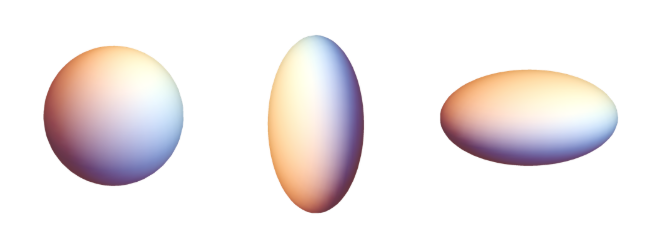
\includegraphics[scale=0.3]{Chapters/Figures/nuclear_shapes.png}
%     \caption{Nuclear Shapes.}
%     \label{nuclear_shapes}
% \end{figure}

The spherical shell model only describes nuclei near the closed shells. On the other side, for the nuclei that lie far from closed shells, a deformed potential must be employed. 
\par In the case of even-even nuclei, unique band structures resulting from the vibrations and rotations of the nuclear surface (as proposed by Bohr and Mottelson \cite{bohr1998nuclear} in the \emph{Geometric Collective Model} - GCM) appear in the energy range 0-2 MeV.

Within the GCM, the nucleus is described as a classical charged liquid drop. For the low-lying energy spectrum, usually, the compression of nuclear matter and the nuclear skin thickness are neglected. This results in the final picture of a liquid drop with a constant nuclear density and a sharp surface \cite{greiner1996nuclear}.

\subsection{Collective coordinates}

The nuclear surface can be described via an expansion of the spherical harmonic functions with some time-dependent parameters as \emph{expansion coefficients}. The expression of the nuclear shape is shown below \cite{greiner1996nuclear}:
\begin{align}
    R(\theta,\varphi,t)=R_0\left(1+\sum_{\lambda=0}^\infty\sum_{-\lambda}^\lambda\alpha_{\lambda\mu}(t)Y_\lambda^\nu(\theta,\varphi)\right)\ .
    \label{nuclear-shape}
\end{align}

In \ref{nuclear-shape}, $R$ denotes the nuclear radius as a function of the spherical coordinates $\theta,\varphi)$ expressing the direction, and the time $t$, while $R_0$ is the radius of the spherical nucleus when all the expansion coefficients vanish. It is worth mentioning that the expansion coefficients $\alpha_{\lambda\mu}$ act as \emph{collective coordinates} since the time-dependent amplitudes describe the vibrations of the nuclear surface.

\subsection{Nuclear radius under rotation}

To get a grasp at the physical meaning behind the deformation parameters that are used to describe the nuclear surface, it is instructive to see what happens when the system undergoes a rotation transformation.

The function $R(\theta,\varphi)$ describes the original (non-rotated) nuclear shape. Rotating the system will result in the change of the angular coordinates $(\theta,\varphi)$ to $(\theta',\varphi')$, which will correspond to a new function $R'(\theta',\varphi')$. Moreover, both nuclear surfaces (i.e., the non-rotated and the rotated one) must hold the equality:
\begin{align}
    R'(\theta',\varphi')=R(\theta,\varphi)
\end{align}

The rotational invariance of $R$ employs that $R'(\theta,\varphi)$ must have the same functional form, but the expansion coefficients $\alpha_{\lambda\mu}$ must be rotated, meaning:
\begin{align}
    \sum_{\lambda\mu}\alpha_{\lambda\mu}'Y'_{\lambda\mu}(
        \theta,\varphi)=\sum_{\lambda\mu}\alpha_{\lambda\mu}Y_{\lambda\mu}(
            \theta,\varphi)\ . \label{nuclear_surface_equality}
\end{align}

Note that in Eq. \ref{nuclear_surface_equality}, the spherical harmonics $Y'_{\lambda\mu}$ are obtained via the usual rotation matrices. Finally, the invariance of Eq. \ref{nuclear-shape} is achieved if the set of parameters $\alpha_{\lambda\mu}$ transform similarly to a \emph{spherical tensor with angular momentum} $\lambda$ \cite{ring2004nuclear}, that is:
\begin{align}
    \alpha_{\lambda\mu}'=\sum_{\mu'}\mathcal{D}^{(\lambda)}_{\mu\mu'}\alpha_{\lambda\mu'}\ .
\end{align}

Besides the spherical tensor character, the collective coordinates also have the following properties (emerging from Eq. \ref{nuclear-shape}):
\begin{itemize}
    \item Complex Conjugation.
    \begin{align}
        Y^*_{\lambda\mu}(\theta,\varphi)&=(-1)^{\mu}Y_{\lambda-\mu}(\theta,\varphi), \\
        \alpha^*_{\lambda\mu}&=(-1)^\mu\alpha_{\lambda-\mu}\ .
    \end{align}
    \item Parity - the coordinates $\alpha_{\lambda\mu}$ must undergo the same change of sign under a parity transformation as the spherical harmonics, in order to keep the invariance of the nuclear surface.
    \begin{align}
        (r,\theta,\varphi) &\xrightarrow[P]{}     (r,\pi-\theta,\pi+\varphi)\ \nonumber, \\
        Y_{\lambda\mu}(\theta,\varphi) &\xrightarrow[P]{} Y_{\lambda\mu}(\pi-\theta,\pi+\varphi)=(-1)^\lambda Y_{\lambda\mu}(\theta,\varphi)\ .\nonumber
    \end{align}
    Therefore, the parity of the expansion coefficients are:
    \begin{align}
        \pi(\alpha_{\lambda\mu})=(-1)^\lambda\ .
    \end{align}
\end{itemize}

\subsection{Multipole deformations}

In the expansion of the nuclear surface defined by Eq. 
\ref{nuclear-shape}, the different values for $\lambda$ will determine different effects regarding the physical aspects of the nucleus. As such, the first values of $\lambda$ will be examined in terms of the physical meaning.

\begin{description}
    \item[Monopole mode] This corresponds to the first value of $\lambda=0$. This is the simplest mode of \emph{deformation} of a nuclear surface. Within this approximation, the spherical harmonic $Y_0^0$ is constant, which would imply that any non-vanishing values for $\alpha_{00}$ will correspond to the change in radius of the nucleus. This kind of excitation is also called \emph{breathing mode} of the nucleus \cite{greiner1996nuclear,bohr1998nuclear}. The energy required for this kind of excitation mode is very large, since it implies a compression of the nuclear matter. As a result, this mode is irrelevant in the low-lying excited spectra of atomic nuclei.
    \item[Dipole mode] Corresponds to $\lambda=1$. In reality, this type of mode does not manifest itself as a deformation of the nucleus, but rather as a shift of the nuclear center of mass. In the lowest order $\lambda=1$, the shift is in fact a translation of the entire nucleus, and it does not represent an actual nuclear excitation.
    \item[Quadrupole mode] Excited modes that correspond to $\lambda=2$. These are the most important collective excitations that take place inside the nucleus. The loss of axial symmetry, triaxial deformations, and other shape-specific transitions that happen within the nucleus are mostly described (and very accurately) via the quadrupole effects.
    \item[Octupole mode] This corresponds to the next increasing value of $\lambda=3$, representing the main asymmetric excitations of a nucleus with states of negative-parity. The specific shape of a nuclear system governed by octuple deformations is similar to that of a pear.
    \item[Hexadecupole deformations] Excitations which correspond to $\lambda=4$. Within the nuclear theory, this is considered the highest angular momentum which can still provide relevant information for the nuclear phenomena that are studied. Currently, there is no clear evidence for pure excitations with hexadecupole nature, however, these excitations seem to have a major role in the admixture to quadrupole excitations for the ground-state shape of heavy nuclei \cite{greiner1996nuclear}.
\end{description}
The multipole deformations for the cases $\lambda=1,2,3$ and $\lambda=4$ discussed above are pictorially shown in Fig. \ref{multipole-deformations}.
Excitations with higher angular momentum than the mentioned ones have practically no application within the study of atomic nuclei. Moreover, one can also see that there is an intrinsic limitation on the maximal value of $\lambda$, which dictates the smallness of the individual bumps of the surface (see Fig. \ref{multipole-deformations}). These bumps are described by the spherical harmonics $Y_\lambda^\mu$, and they decrease in size with increasing values of $\lambda$, but with the physical limitation given by the size of the nucleon diameter.

\begin{figure}
    \centering
    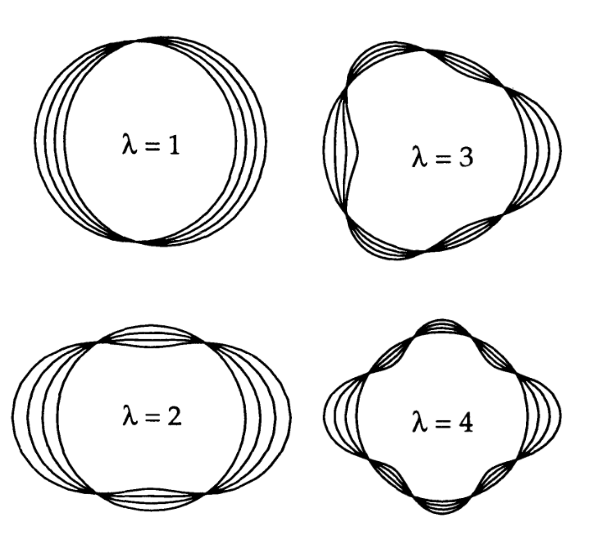
\includegraphics[scale=0.3]{Chapters/Figures/nuclearDeformation.png}
    \caption{Graphical representation for the first few modes of excitations of the nuclear surface. The figure is taken from Ref. \cite{greiner1996nuclear}.}
    \label{multipole-deformations}
\end{figure}

\subsection{Quadrupole Deformation}

One of the most important excitation modes (vibrational degrees of freedom) is the quadrupole deformation, corresponding to $\lambda=2$. In the case of pure quadrupole deformation, the nuclear surface will be given by the following expression:
\begin{align}
    R(\theta,\varphi)=R\left(1+\sum_\mu\alpha_{2\mu}Y_2^\mu(\theta,\varphi)\right)\ . \label{quadrupole-surface}
\end{align}

From this expression, the term $\alpha_{00}$ is of second order in $\alpha_{2\mu}$ and it can be neglected further on. This term also reflects the conservation of volume \cite{greiner1996nuclear,ring2004nuclear}. The real and independent degrees of freedom from the above expression are: $\alpha_{20}$, the real and imaginary parts of $\alpha_{21}$, and the real and imaginary parts of $\alpha_{22}$, respectively.

More insight with regards to the quadrupole shape of the nucleus can be achieved if one expresses $R$ in terms of cartesian coordinates. The spherical harmonics will attain a new form, depending on the cartesian components of the unit vector pointing in a direction defined by $(\theta,\varphi)$:
\begin{align}
    \xi=\sin\theta\cos\varphi\ ,\ \eta=\sin\theta\sin\varphi\ ,\ \zeta=\cos\theta\ ,
\end{align}
with the condition $\xi^2+\eta^2+\zeta^2=1$. With the expressions of the spherical harmonics as functions of $(\xi,\eta,\zeta)$, the nuclear radius will change accordingly (cartesian expression $R=R(\xi,\eta,\zeta)$). A relationship between the cartesian components and the spherical ones for the deformation can be also obtained if one writes all coefficients $\alpha_{2\mu}$ as functions of $\alpha_{ij}$ (with $i,j=\xi,\eta,\zeta$). Since the cartesian deformations can be regarded as closely related to a stretch/contraction of the nucleus in a given direction, a first interpretation of the physical meaning behind the parameters $\alpha_{2\mu}$ can be established:
\begin{itemize}
    \item $\alpha_{20}$: describes the stretching of the $z$ axis with respect to the $y$ and $x$ axes.
    \item $\alpha_{2-2}$ and $\alpha_{22}$: give the relative length of the $x$ axis compared to the $y$ axis. Moreover, it also gives the oblique deformation in the $x-y$ plane.
    \item $\alpha_{2-1}$ and $\alpha_{21}$: describe an oblique deformation, but with respect to the $z$ axis.
\end{itemize}

With the set of parameters defined above, the shape and orientation of the nucleus can have arbitrary values (the coefficients $\alpha_{2\mu}$ are mixing the shape and orientation), thus making the parametrization somewhat problematic. In order to fix that, the geometry can be changed if one considers the \emph{principal axis system} (the PA reference system is a coordinate system in which the moments of inertia associated with the nucleus are diagonal). 
When using this reference frame, the number of parameters is still unchanged, however their physical significance becomes clearer. By denoting the new coordinate system with primed letters, nuclear radius will be described as a function $R=R(\xi',\eta',\zeta')$, with the conditions that $\alpha'_{ij}=0\ ,\ i\neq j$. The condition will further imply that the newly expressed parameters ($\alpha'_{2\mu}$) have the following form:
\begin{align}
    \alpha'_{2 \pm 1}&=0\ , \nonumber \\
    \alpha'_{2 \pm 2}&\equiv a_2\ , \nonumber \\
    \alpha'_{20}&\equiv a_0\ . 
\end{align}
, where the conveniently denoted terms $a_2$ and $a_0$ are some functions that depend on the cartesian components $\alpha_{\xi,\xi}\ ,\ \alpha_{\eta,\eta}\ ,\ \alpha_{\zeta,\zeta}$. From this set of equations the physical significance of the five real and independent parameters is clearer:
\begin{itemize}
    \item $a_0$ is indicating the stretch of $z'$ axis w.r.t. the $x'$ and $y'$ axes.
    \item $a_2$ is indicating the asymmetry between the lengths of $x'$ and $y'$ axes respectively.
    \item the Three \emph{Euler angles} $\mathbf{\theta}=(\theta_1,\theta_2,\theta_3)$. These angles will determine the orientation of the PA system $(x',y',z')$ with respect to the laboratory-fixed frame $(x,y,z)$.
\end{itemize}

One can now clearly see the advantage of working within the PA system: rotation and shape vibration degrees of freedom can be completely separated. A change in the Euler angles will result in a pure rotation of the nucleus (without changing its shape), while a change in shape will be affected exclusively by the $a_0$ and $a_2$ parameters. If $a_2=0$, then the nucleus has a shape with axial symmetry around the $z$ axis (equal axis lengths along the $x$ and $y$ directions).

Another way of describing the excitations of quadrupole type is to adopt the parameters introduced by A. Bohr \cite{bohr1954rotational}. These two parameters can be viewed as a set of polar coordinates in the space generated by $(a_0,a_2)$ and they are defined as:
\begin{align}
    a_0&=\beta_2\cos\gamma\ , \nonumber \\
    a_2&=\frac{1}{\sqrt{2}}\beta_2\sin\gamma\ , \label{bohr-deformation-params}
\end{align}
where the numeric factor $\frac{1}{2}$ was added such that the following relation holds true:
\begin{align}
    \sum_\mu\left|\alpha_{2\mu}\right|^2=\sum_\mu\left|\alpha'_{2\mu}\right|^2=a_0^2+2a_2^2=\beta_2^2\ .
    \label{quadrupole-param-sum}
\end{align}
It is worth mentioning that the Eq. \ref{quadrupole-param-sum} is rotationally invariant, having the same value in the laboratory and the principal axes systems.

Now that the shape of the nucleus (i.e., the nuclear surface radius $R$) can be described consistently with via the parameters defined in Eq. \ref{bohr-deformation-params}, one can calculate the stretching of the nuclear radius along any of the directions is given in terms of $(\beta,\gamma)$ as follows:
\begin{align}
    \delta R_k=\sqrt{\frac{5}{4\pi}}\beta\cos(\gamma-\frac{2\pi k}{3})\ .
\end{align}

\subsubsection{Axial quadrupole deformations}

Using this set of new coordinates, the expression of the nuclear radius for axially quadrupole-deformed nuclei is given as:
\begin{align}
    R(\theta,\varphi)=R_0\left(1+\beta_2 Y_2^0(\theta,\varphi)\right)\ . \label{quadrupole-radius}
\end{align}

In Eq. \ref{quadrupole-radius}, the parameter $\beta_2$ is called the \emph{quadrupole deformation parameter}, and its value dictates wether the nucleus is \emph{oblate} - $\beta_2<0$ (i.e., a flattened sphere), \emph{prolate} - $\beta_2>0$ (i.e., elongated sphere, like a rugby ball), or \emph{spherical} - $\beta_2$.  The nuclear shapes that are characterized only by $\beta_2$ (i.e., $\gamma=0$) have shapes that correspond to spheroids. These shapes are axially symmetric, meaning that they only have one deformed axis. For the spherical case $\beta_2=0$, all three axes have the same lengths, meaning that the shape of the nucleus is in fact a sphere.

For the axially-symmetric quadrupole deformations, the parameter $\beta_2$ can be related to the axes of the spheroid via the formula \cite{greiner1996nuclear}:
\begin{align}
    \delta R_k=\sqrt{\frac{5}{4\pi}}\beta_2\cos\left(\gamma-\frac{2\pi k}{3}\right)\ ,
\end{align}
with $k=1,2,3$ indices that correspond to each of the three principal axes $x'$, $y'$, and $z'$, respectively. The stretching of the nuclear axis in a particular direction (denoted by $k$ in the above formula) varies according to the change in $\gamma$, for a fixed value of $\beta_2$.

\begin{figure}
    \centering
    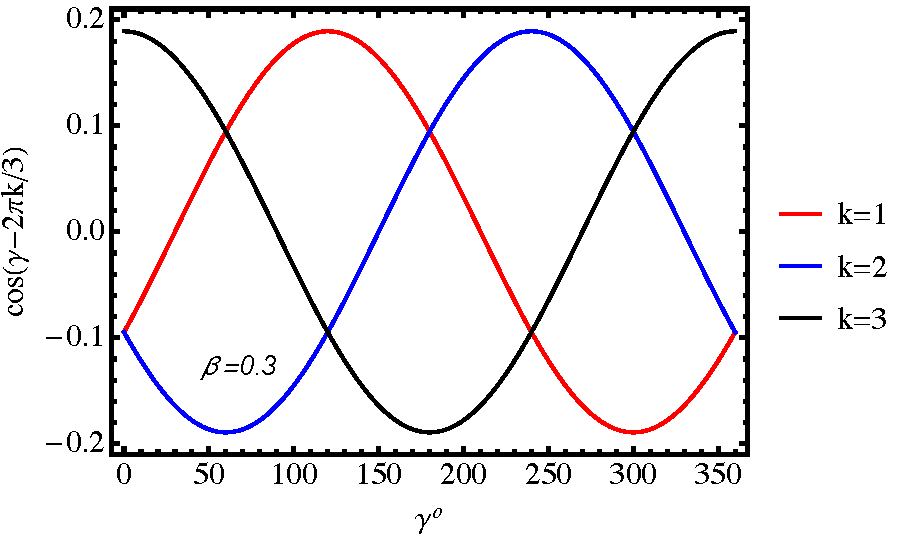
\includegraphics[scale=0.65]{Chapters/Figures/nuclear-radius-elongation.pdf}
    \caption{A graphical representation with the stretching of the nuclear axis $\delta R_k$ for $k=1,2,3$, corresponding to the increase in axis lengths along the $x$, $y$, and the $z$ directions, respectively. The representation used an arbitrary value for the quadrupole deformation $\beta_2=0.3$. Figure was reproduced according to the calculations done in \cite{greiner1996nuclear}.}
    \label{nuclear-radius-elongation}
\end{figure}

Taking a look at Fig. \ref{nuclear-radius-elongation}, one can see the variations of the three axes with $\gamma$. When $\gamma=0^\circ$ the nucleus is elongated along the $z'$ axis, but the $x'$ and $y'$ axes are identical (the prolate case) - axial shape. As $\gamma$ increases, the $x'$ axis grows, while the other two axes decrease in size, making a region with \emph{triaxial shapes} - all three axes are unequal in magnitude. Symmetry is reached again at $\gamma=60^\circ$, however the $x'$ and $z'$ axes are equal this time but longer than $y'$ axis, making the nucleus look like a flattened shape (the oblate case) - axial shape. This pattern is repeated every $\gamma=60^\circ$, where axial shapes emerge, with alternating prolate/oblate shapes.

It is possible to summarize the various nuclear shapes that can occur with the help of a diagram done in the $(\beta,\gamma)$ plane.

\subsubsection{Non-Axial quadrupole deformations}
 % Chapter 2
\chapter{Nuclear Models}

\section{Introduction}

In the following, it is worth to make a discussion about the nuclear models that are used by theoreticians in order to describe phenomena that are specific to rotating nuclei and high-spin regime. Since the focus of this work emerges from a \emph{class} of properties that usually apply to the high-spin region (but this does not necessarily also imply a high-energy region), it makes sense to give an insight in the tools that fit the best the underlying effects.

\section{Shell model}

The fact that an atomic nucleus can have a structure that behaves rather similarly as its \emph{parent} (i.e., the atom) in terms of changing the number of constituents, has been enforced by the experimental observations that were done across time. The sharp and discrete discontinuities of nuclear properties, such as the nucleon separation energy, point to the fact that nucleus can be explained through the existence of \emph{shells}. Some examples of observations which indicate this are:
\begin{itemize}
    \item When adding a nucleon to a nucleus, there are certain places where the \emph{binding energy} of the next nucleon becomes considerably smaller than the previous one. 
    \item Separation energies for both the protons and neutrons suffer drastic changes, having strong deviations from the predictions of the semi-empirical mass formula \cite{weizsacker1935theorie}, the discontinuities being represented by major shell closures (complete filling) \cite{krane1991introductory}.
    \item The neutron absorption cross-section has a substantial decrease in value at the neutron magic numbers
    \item Great abundance of nuclides where $Z$ and $N$ are magic numbers.
\end{itemize}

The sudden discontinuities occur at specific values of the proton $Z$ and neutron $N$ numbers: these are called \emph{magic numbers}. Currently, these magic numbers correspond to $Z$ or $N=2,8,20,28,50,82,126$, and they represent the so-called major shells. There are also two \emph{weakly magic numbers}: 40 and 64.

One can examine the values for the first excited states $2^+$ that are shown in Figs. \ref{e2plus_proton}, \ref{e2plus_neutron}. Indeed, these values show some peaks, each peak corresponding to a particular magic number. This results are part of the work of Raman et al \cite{raman2001transition}, where the transition probabilities from the ground state to the first-excited $2^+$ state in even-even nuclei were evaluated.

\begin{figure}
    \centering
    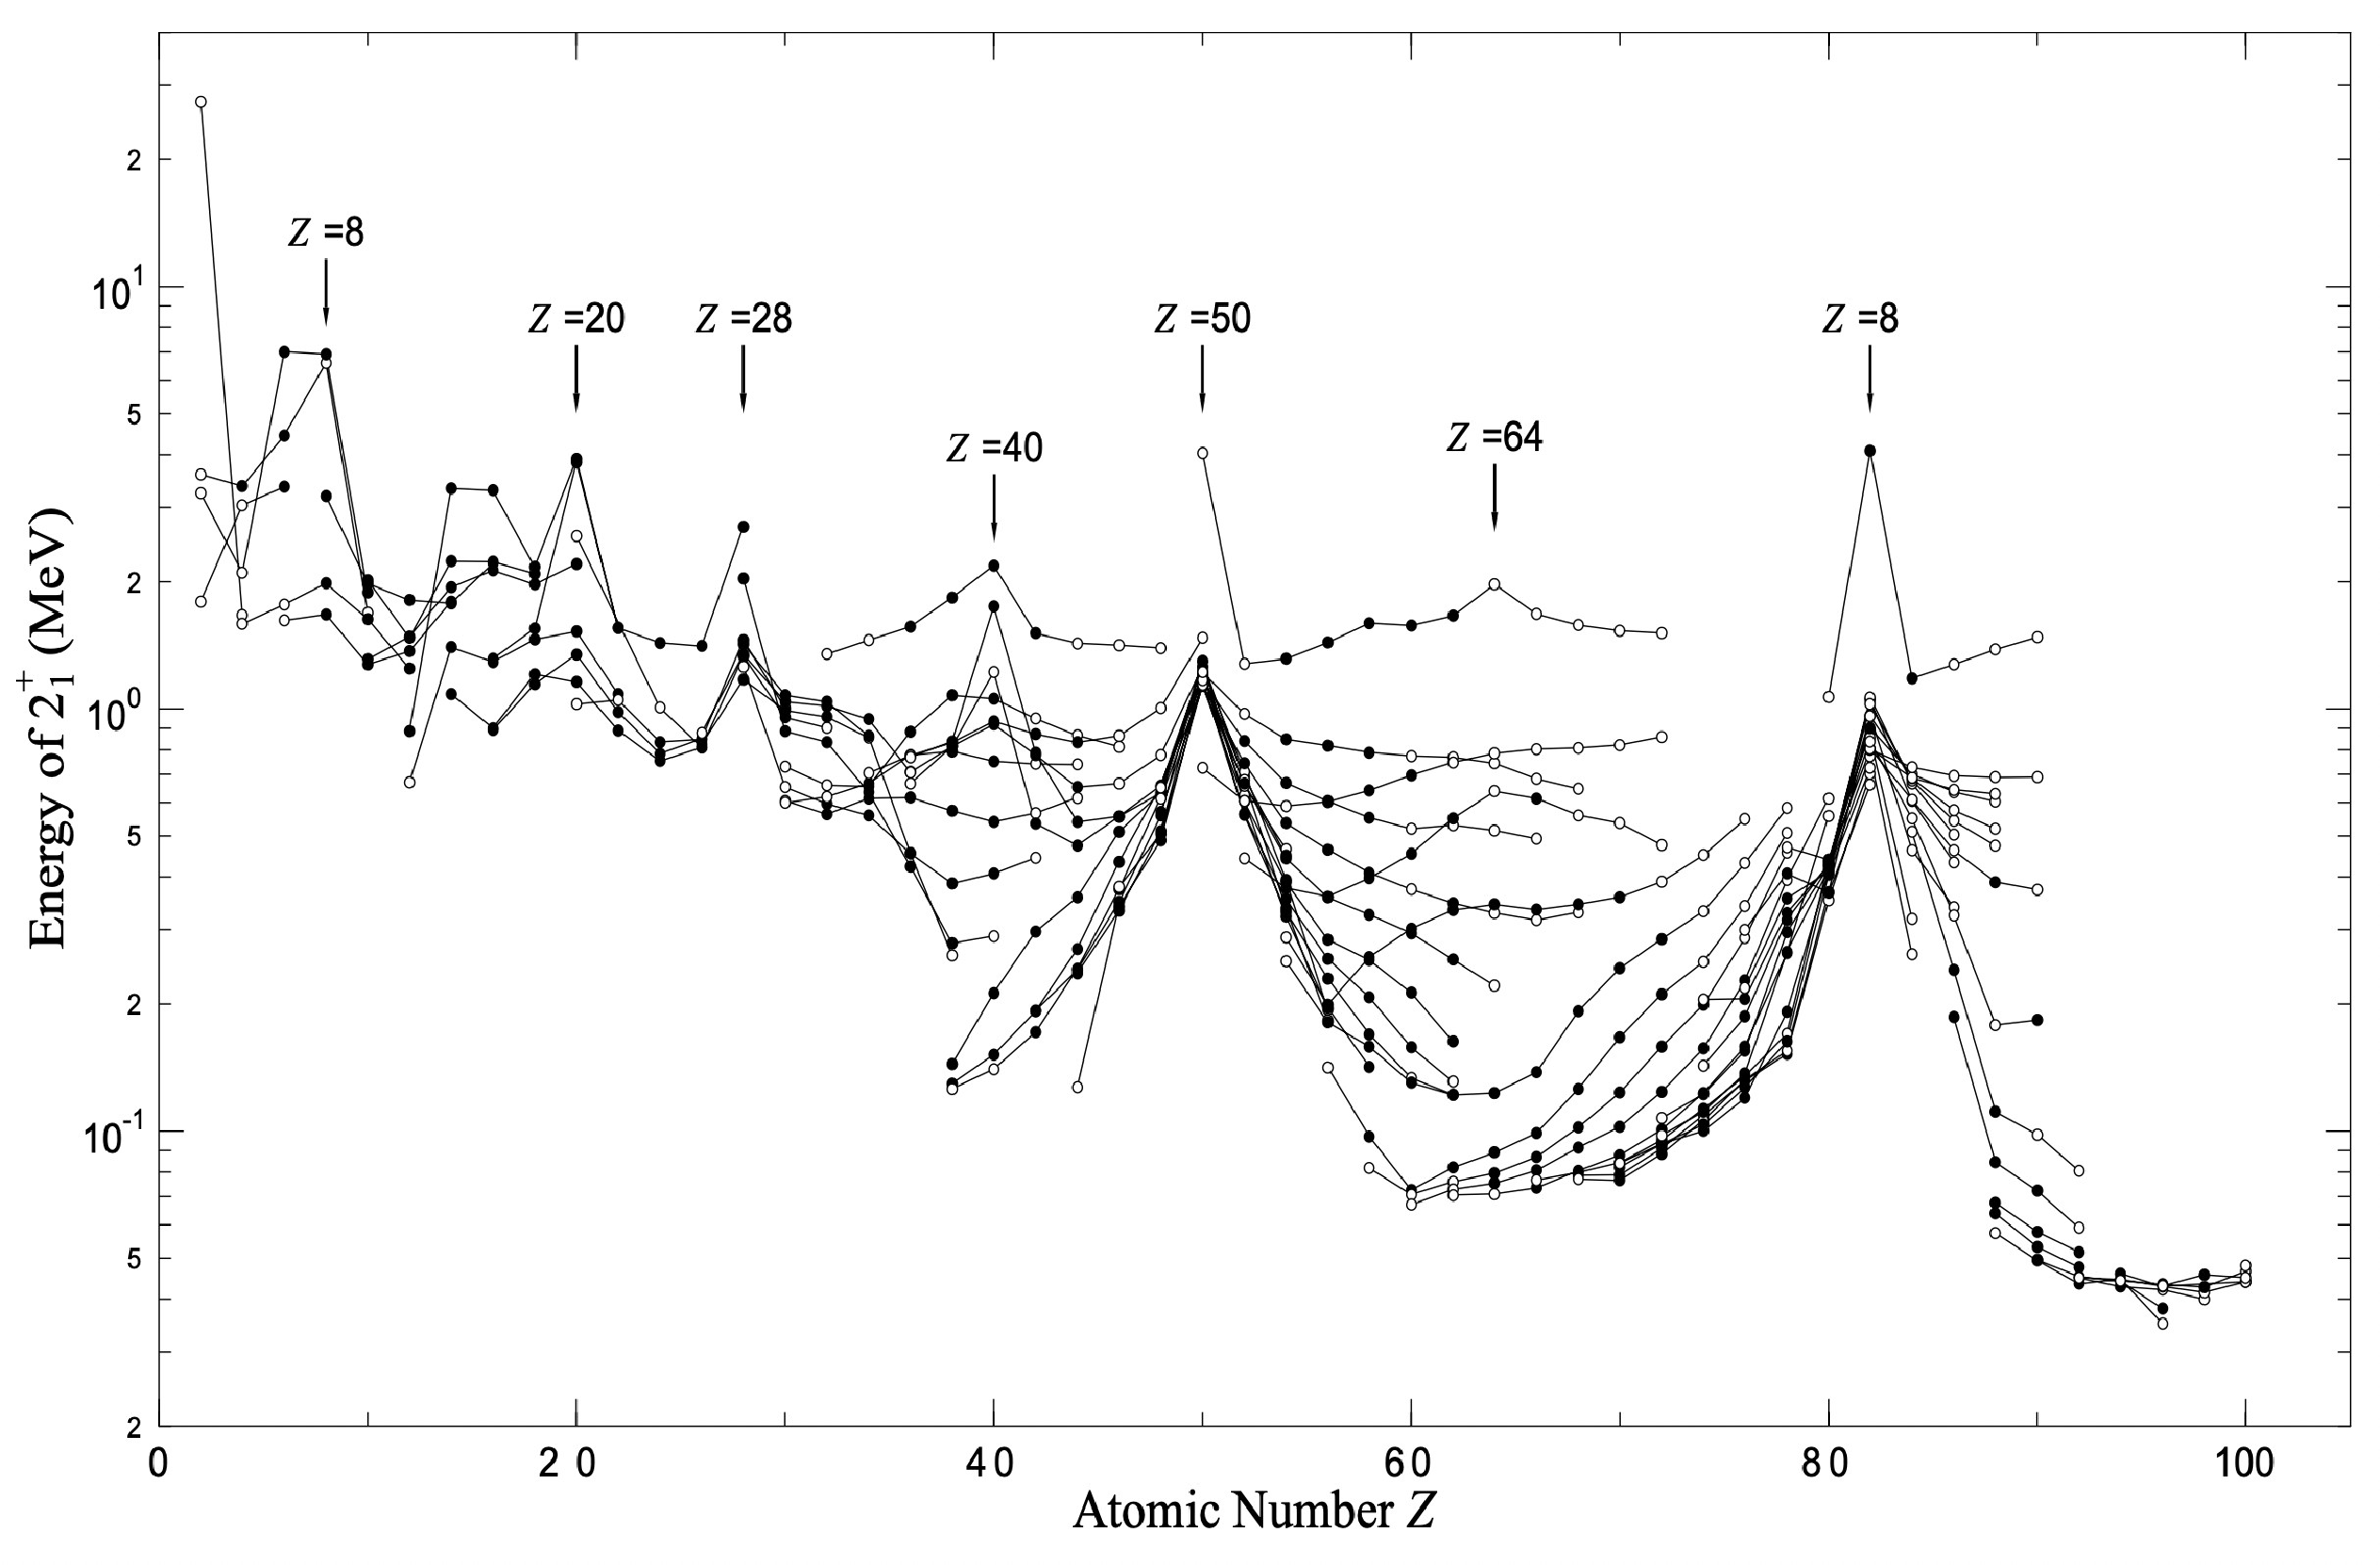
\includegraphics[scale=0.33]{Chapters/Figures/E2plus_proton.pdf}
    \caption{The first excited energy states $2^+$ of nuclei with even $Z$ and $N$ graphically represented with respect to the proton number. Each line represents a set of isotopes. Figure taken from Ref. \cite{matta2017exotic}.}
    \label{e2plus_proton}
\end{figure}

\begin{figure}
    \centering
    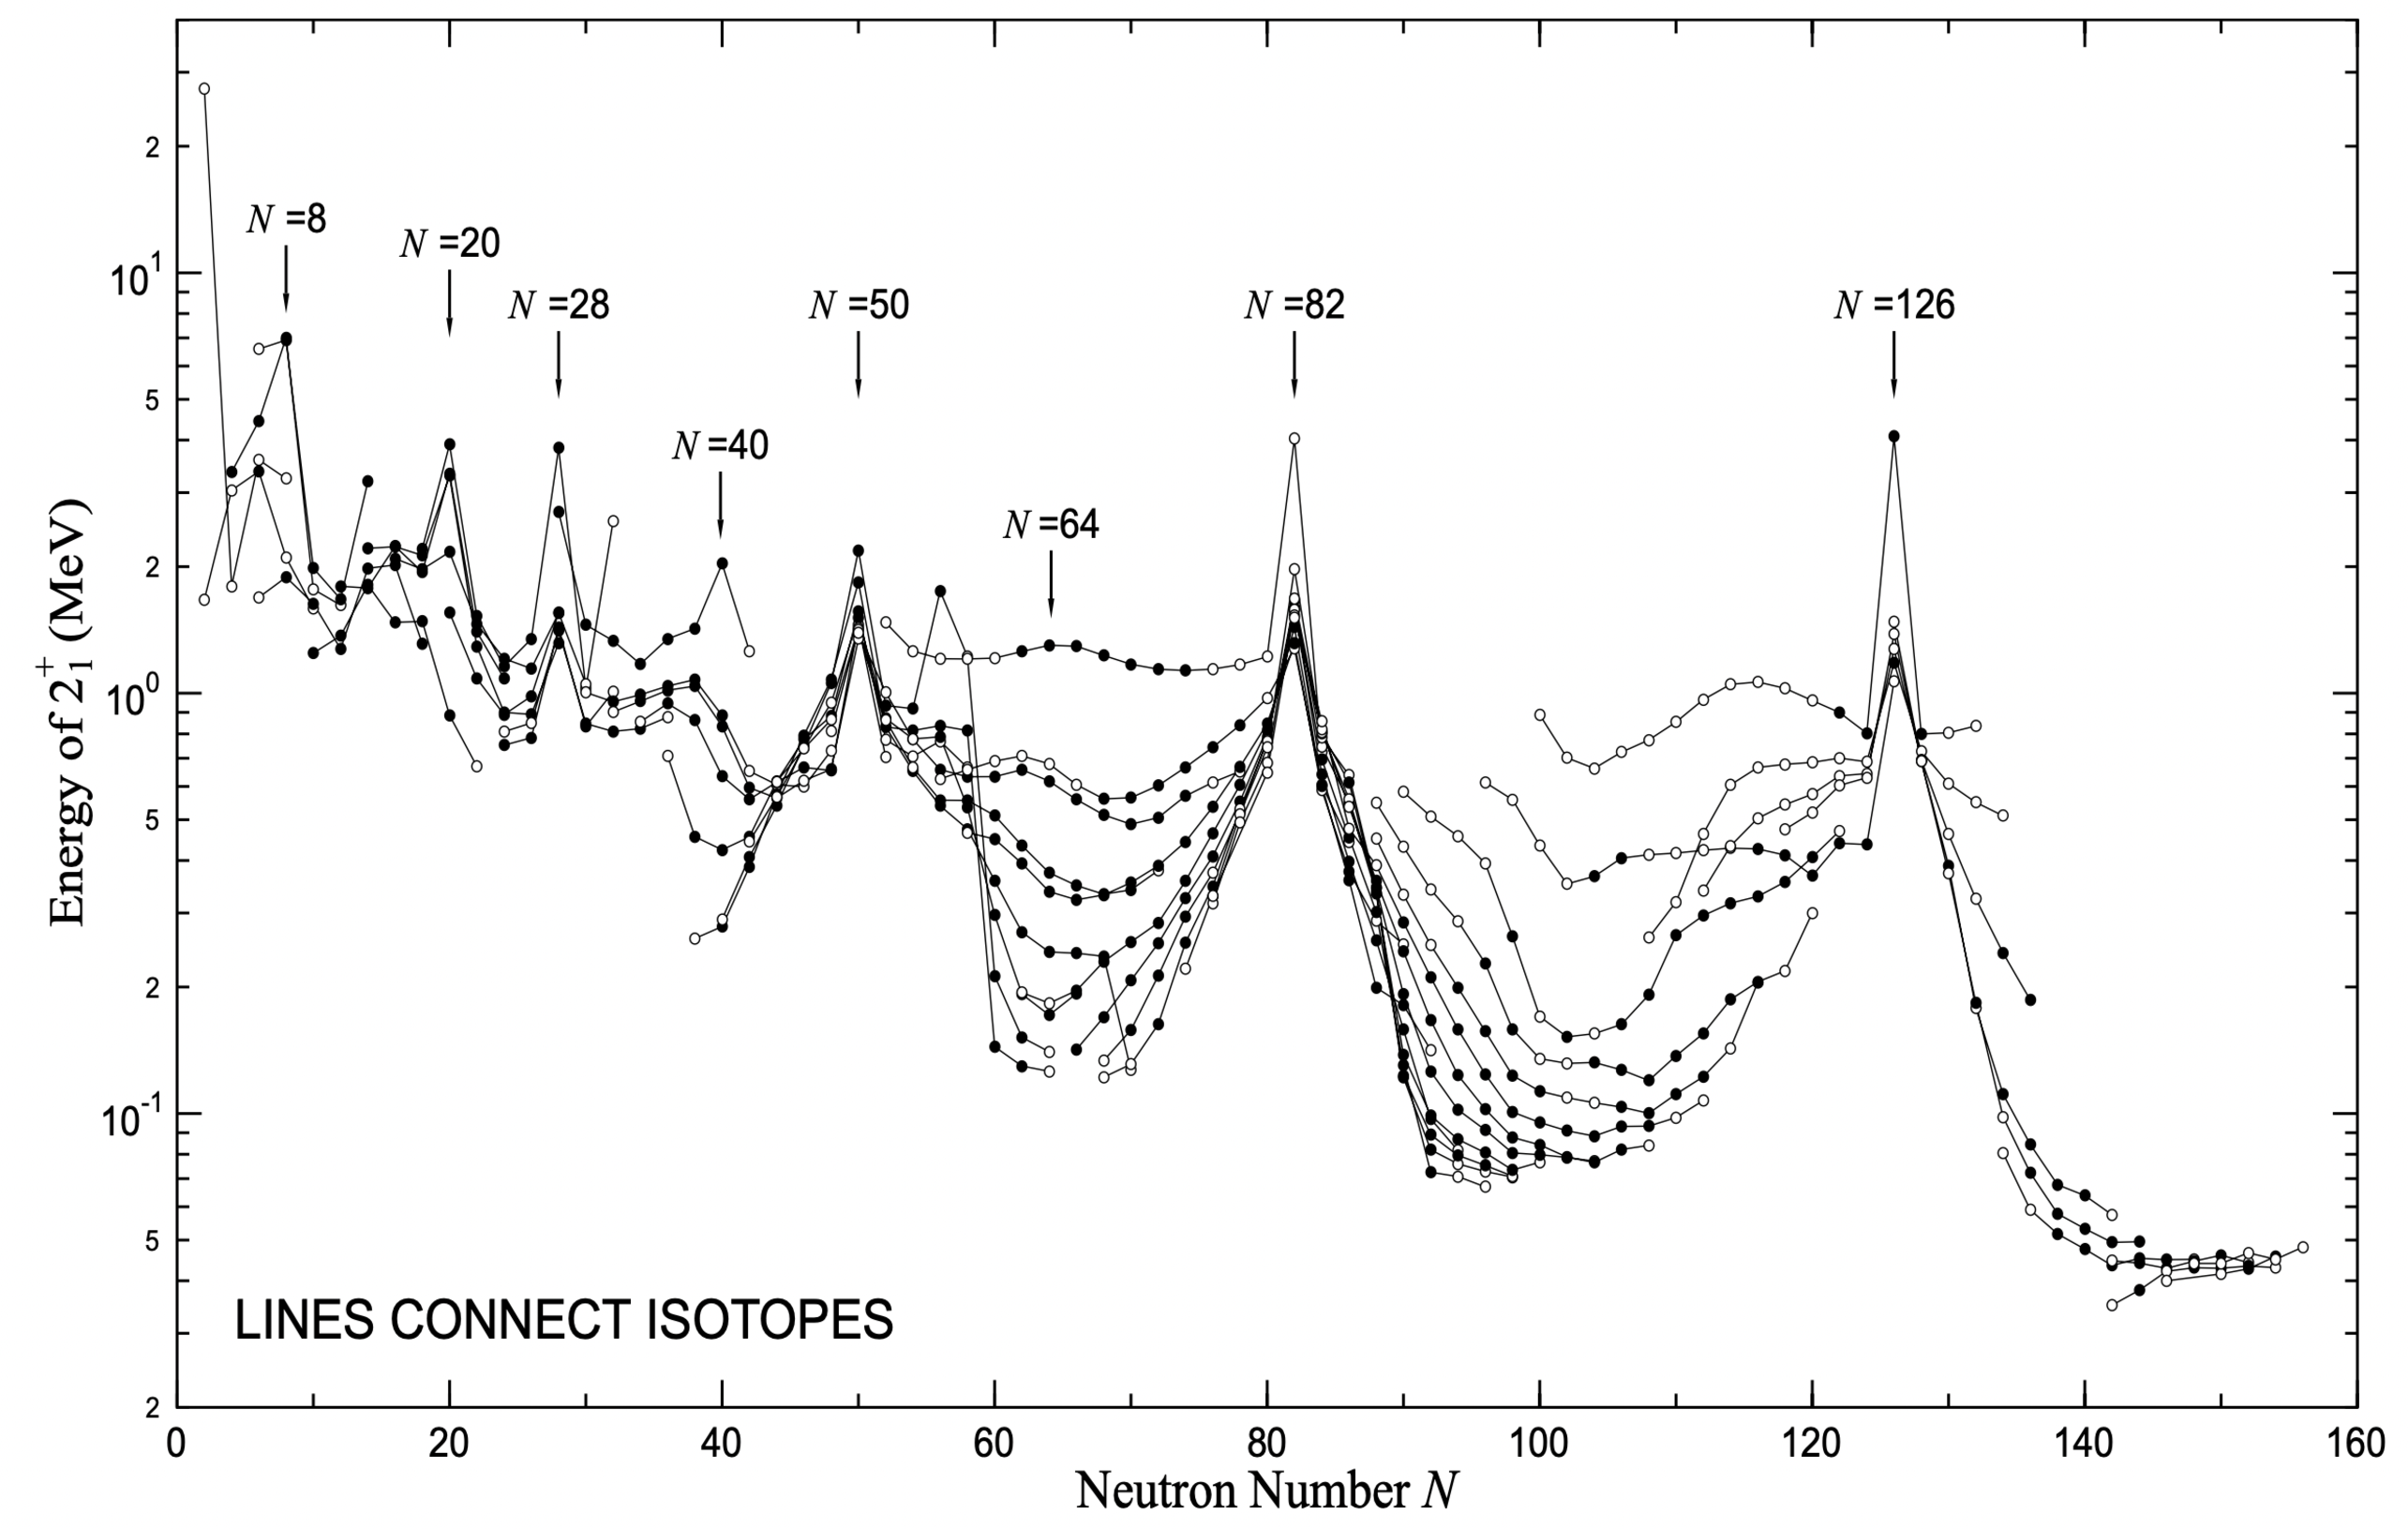
\includegraphics[scale=0.33]{Chapters/Figures/E2plus_neutron.pdf}
    \caption{The first excited energy states $2^+$ of nuclei with even $Z$ and $N$ graphically represented with respect to the neutron number. Each line represents a set of isotopes. Figure taken from Ref. \cite{matta2017exotic}.}
    \label{e2plus_neutron}
\end{figure}

The shell model starts from the basic assumption that the nucleus is a \emph{mean-field potential}, that is a potential for which the motion of a single nucleon is caused by all the other nucleons (the nucleon is moving inside an average potential generated by all the other constituents of the nucleus). Of course, all the nucleons that are under the influence of such a mean field potential occupy the energy levels which correspond to a series of (sub)shells that agree with the Paul exclusion principle. Having a general expression for the potential that properly reproduces all the magic numbers (and the observed nuclear properties) is the main goal.

Since the model starts from the concept of independent (non-interacting) particle motion within an average potential, finding each energy will be equivalent of solving the Schrödinger equation:
\begin{align}
    -\frac{\hbar^2}{2m}\nabla ^2\psi_i(r)+V(r)\psi_i(r)=e_i\psi_i(r)\, 
    \label{schrodinger-single-particle-eq}
\end{align}
where $e_i$ represents the energy (eigenvalue) and $\psi_i$ represents the wave-function (eigenstates), while $V(r)$ is the nuclear potential whose expression must be evaluated.

The choice of $V(r)$ will be dictated by the reproduction of various experimental data (such as nuclear saturation, scattering, nuclear reactions, and so on). For the motion of an independent particle, an obvious first attempt would be the \emph{simple harmonic oscillator} (SHO), which has the known expression:
\begin{align}
    V(r)=\frac{1}{2}m(\omega_i r)^2\ ,
    \label{harmonic-potential}
\end{align}
with $\omega_i$ as the frequency of the basic harmonic-like motion of the particle in the nucleus. With Eq. \ref{harmonic-potential}, the motion of the nucleon has a straightforward expression:
\begin{align}
    \frac{\hbar^2}{2m}\nabla^2\psi_i(r)+\frac{1}{2}m(\omega r)^2\psi_i(r)=e_i\psi_i(r)\ .
\end{align}

This Schrödinger equation has its energy eigenvalues under to form:
\begin{align}
    e_N=\left(N+\frac{3}{2}\right)\hbar\omega\ ,
\end{align}
where $N$ is the number of oscillator quanta which describes each major shell (also called the \emph{principal quantum number}). One should keep in mind that such an expression is typical for a three-dimensional and isotropic harmonic oscillator. The principal quantum number $N$ is furthermore defined as:
\begin{align}
    N=2(n-1)+l\ ,
\end{align}
with $n$ and $l$ being the \emph{radial} quantum number and \emph{orbital angular momentum} quantum number, respectively, taking values $n=1,2,3,\dots$ and $l=0,1,2,\dots,n-1$. In this first approximation, all the levels with the same principal quantum number $N$ are \emph{degenerate}, with a maximal degeneracy given by $2(2l+1)$. However, by using only the SHO term as the expression of $V(r)$, only the first three magic numbers are reproduced, meaning that some additional term(s) might be needed in order to consistently obtain the series of magic numbers.

A next step is to use the fact that the experimentally observed short range of the strong nuclear force: the steepness of the SHO can be corrected with an \emph{attractive} term proportional to $l$-squared. This acts as a centrifugal term which provides an angular momentum barrier, lifting the degeneracy between the levels with the same principal quantum number $N$ and different values for the orbital angular momentum $l$. This SHO+$l^2$ step is still not enough though. The last step is to add a so-called \emph{spin-orbit} coupling term of the form $\vec{l}\cdot\vec{s}$. 
% This last term is enough to reproduce all the magic numbers and the experimentally measured quantities that are relevant to the shell model itself.
This term comes from the consideration that the nucleon-nucleon interaction has a spin dependence, and the potential depends on the intrinsic spin $s$ ($\vec{s}$) and the orbital angular momentum $l$ ($\vec{l}$) of a nucleon. Since $\vec{j}=\vec{l}+\vec{s}$, two possible states emerge from a single value of $l$ (depending on wether $\vec{s}$ is parallel or anti-parallel to $\vec{l}$). The final expression of the terms SHO+$\vec{l}^2$+$\vec{l}\cdot\vec{s}$ will consist in the \emph{Modified Harmonic Oscillator} (HMO).
\begin{align}
    V(r)=\frac{1}{2}(\omega r)^2+B\ \vec{l}^2+A\ \vec{l}\cdot\vec{s}\ .
    \label{modified-harmonic-oscillator-eq}
\end{align}

For the sake of simplicity, the centrifugal term will be denoted within formulas without the vector symbol. Since the intrinsic spin of a nucleon is $s=1/2$, for a given value of $l$, there can be two values for the \emph{total angular momentum} (a.m.) $j=l\pm1/2$: one for each spin orientation with respect to the direction of the orbital a.m. Moreover, for each value of $l=0,1,2,3,4,\dots$, there is a similar notation $l=s,p,d,f,g,\dots$, respectively. Regarding the spectroscopic notation, usually, the value of $j$ is considered as a subscript; $nl_j$ (for example $1p_{1/2}$ and $1p_{3/2}$). What it is worth mentioning is that for high enough shells, there can be splittings between $j+1/2$ and $j-1/2$ that are large enough to lower the $j+1/2$ state from one oscillator shell $n$ to one located below $n-1$. These types of levels are called \emph{intruder states} and they have opposite parity $\pi=(-1)^l$ with respect to the shell that these levels will occupy.

Going back to the expression of the $\vec{l}\cdot\vec{s}$ term from Eq. \ref{modified-harmonic-oscillator-eq} and denoting it with $V_{ls}(r)$, it is shown by Casten \cite{casten2000nuclear} that its contribution to the total potential can be regarded as a surface effect. Due to this, its form can be expressed as a function that depends on the radial coordinate as such \cite{casten2000nuclear}:
\begin{align}
    V_{ls}(r)=-a_{ls}\frac{\partial V(r)}{\partial r}\vec{l}\cdot\vec{s}\ ,
\end{align}
where $V(r)$ is the expression for a central potential and $a_{ls}$ is a strength constant.
% Indeed, in the work of Casten \cite{casten2000nuclear}, it is stated that if in the nucleus, the spin-orbit forces were large enough, then there should be an overall preference for nucleons with spins aligned parallel their orbital a.m. other than the opposite alignment, making the nucleons with anti-parallel spins to not be surrounded by an equal number of nucleons with all spin orientations.

Now that an expression for the nuclear potential that is able to reproduce all the magic numbers has been formulated, it is also possible to formulate the total energy of a single-particle within the average potential that is generated by all the other nucleons within the nucleus. Thus, the Hamiltonian of this simple system (the modified oscillator) can be formulated as such:
\begin{align}
    H&=-\frac{\hbar^2}{2m}\nabla^2+V_\text{SHO}+(l^2)_\text{term}+(\vec{l}\cdot\vec{s})_\text{term}=-\frac{\hbar^2}{2m}\nabla^2+V_\text{MHO} , \nonumber\\
    H&=-\frac{\hbar^2}{2m}\nabla^2+\frac{1}{2}m(\omega r)^2+Bl^2+A\vec{l}\cdot\vec{s}\ .
\end{align}

The evolution from each term in the shell-model potential (that is the first approximation as a SHO, then SHO+$l^2$, and finally SHO+$l^2+\vec{l}\cdot\vec{s}$ or modified oscillator potential) is illustrated in Fig. \ref{energy-levels-mho}, where it can be seen how each extra term introduces a new degeneracy within the energy states, with the complete reproduction of the magic numbers in the third column. Moreover, the \emph{intruder} levels can be observed, where levels with $j=l+1/2$ from a particular $n$ are so low, that they lie below an $n-1$ adjacent level.
\begin{figure}
    \centering
    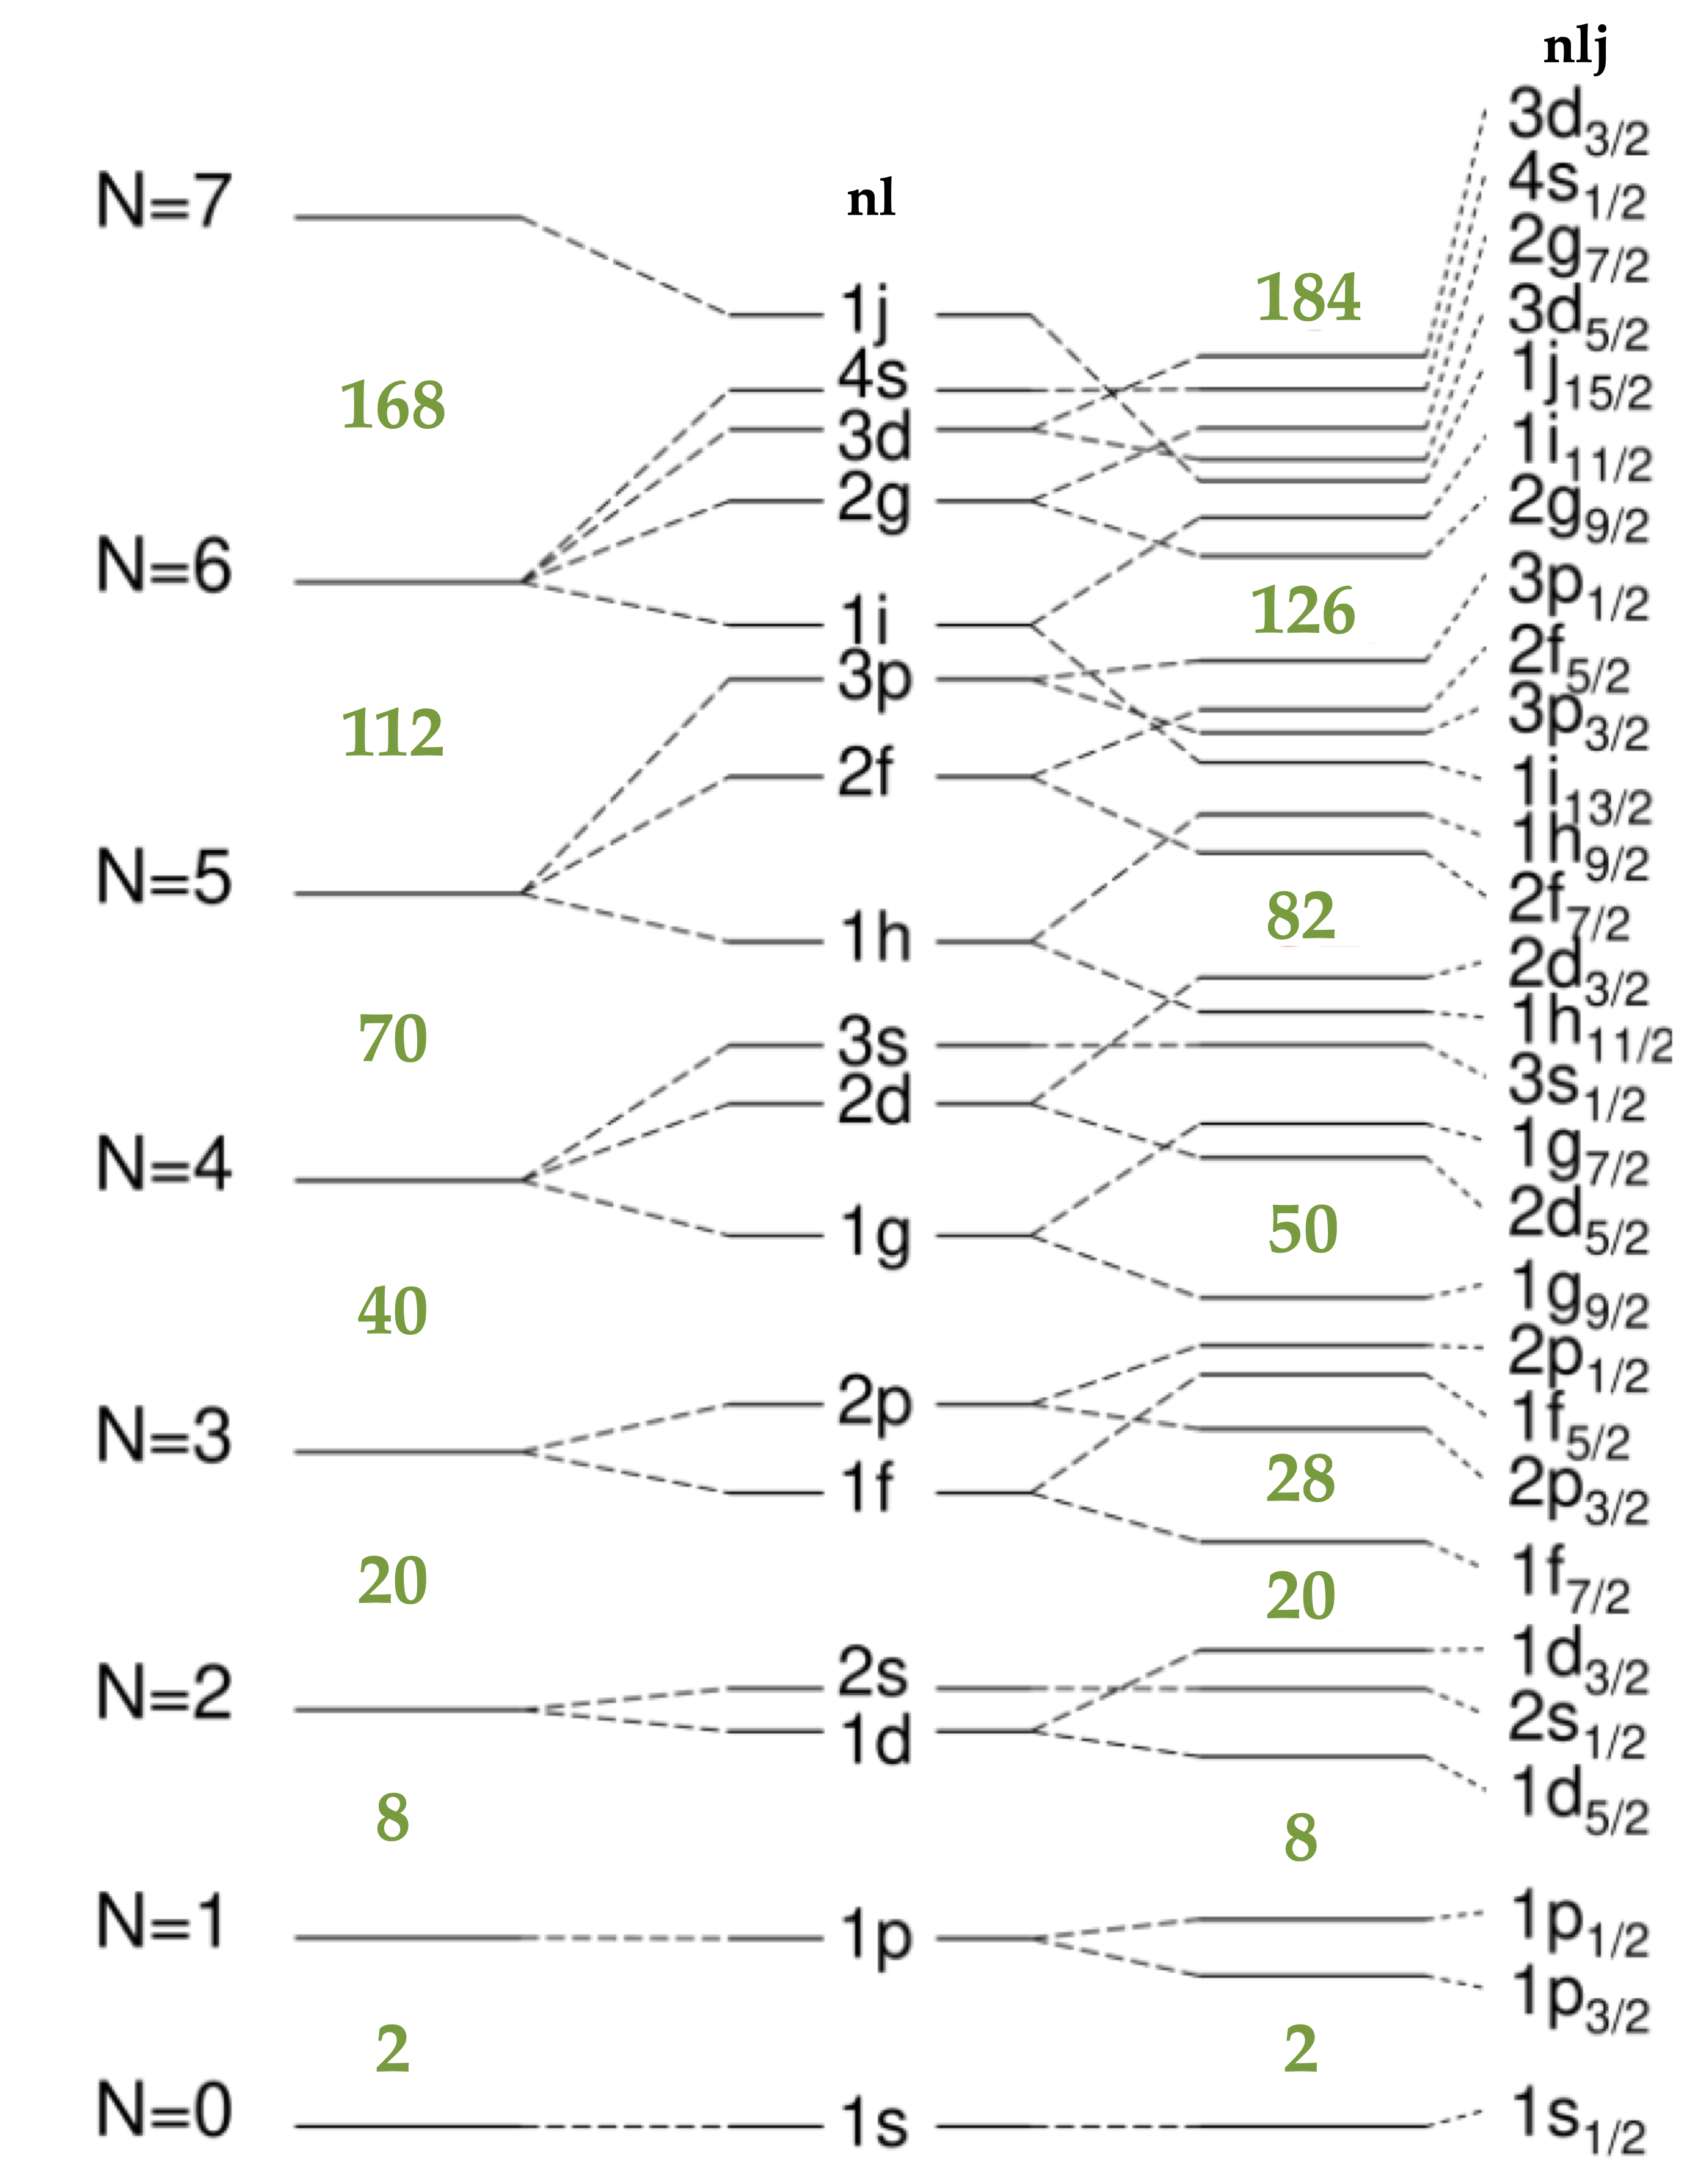
\includegraphics[scale=0.12]{Chapters/Figures/SM_level_scheme.png}
    \caption{The energy levels obtained via calculation of the shell model potential using the simple oscillator (SHO), the SHO amended with a centrifugal term $l^2$, and finally the modified oscillator (MHO) that contains a spin-orbit term. The `correct' magic numbers are the ones in the right-most column. Figure is adapted from Refs. \cite{matta2017exotic},\cite{krane1991introductory}.}
    \label{energy-levels-mho}
\end{figure}

Another, more realistic potential that can be used in order to reproduce the specific shell model calculation is the so-called Woods-Saxon potential. Because of the short-range character of the strong nuclear force, it is safe to assume that this potential should behave in the same manner as the density distribution of the nucleons. Since for medium and heavy nuclei, the Fermi-like functions (distributions) are the ones that best fit the experimentally measured data, this potential should have the following form \cite{woods1954diffuse}:
\begin{align}
    V_\text{ws}(r)=-\frac{V_0}{1+e^{\frac{r-R_0}{a}}}\ .
    \label{woods-saxon-potential}
\end{align}
This mean-field potential contains the terms $V_0$ that represents the depth of the potential ($\approx 50$ MeV, in order to reproduce the experimental separation energies for the nucleons), the surface thickness $a$ (also called the diffuseness parameter, giving information about how fast the potential drops to zero) with a value of approximately $0.5$ fm, while $R_0$ is the nuclear radius with $R_0=r_0A^{1/3}$ and $r_0=1.2$ fm. The nature of this potential is of \emph{central type} and, unfortunately, Eq. \ref{woods-saxon-potential} in its pure form is not enough the reproduce the higher magic numbers. As such, the addition of a spin-orbit term, similarly as in the case of MHO potential, is required \cite{martin2017particle}: 
\begin{align}
    V_\text{total}=V_\text{ws}^\text{central}+V_{ls}(r)\vec{l}\cdot\vec{s}\ .
    \label{woods-saxon-so-potential}
\end{align}
The only good quantum numbers in the case of the WS potential are the total a.m. $j$ and the parity $\pi=(-1)^l$.
The expectation value of the spin-orbit term $\vec{l}\cdot\vec{s}$ can be given as:
\begin{align}
    \langle ls \rangle=\hbar^2\begin{cases}
        \frac{l}{2} \quad &\text{for} j=l+\frac{1}{2}\\
        -\frac{l+1}{2} &\text{for} j=l-\frac{1}{2}\ \\
   \end{cases}\ .
\end{align}
and the spacing between two levels can be furthermore expressed as \cite{martin2017particle}:
\begin{align}
    \Delta E_{ls}=\frac{2l+1}{2}\hbar^2\langle V_{ls}\rangle\ .
\end{align}
The experimental evidence points to the fact that $V_{ls}(r)$ is negative, meaning that states with $j=l-1/2$ are shifted higher than $j=l+1/2$. Some characteristics of the WS potential are the following:
\begin{enumerate}
    \item It increases with the increase of $R$, meaning that it has an \emph{attractive nature}
    \item It flattens out for large enough $A$ in the center of the nucleus
    \item It rapidly goes to zero as $R$ increases (given by the diffuseness parameter), indicating its short-range nature
    \item When $R=R_0$ (that is for the nucleons near the surface), a large force towards the center of the nucleus is experienced by the these nucleons.
\end{enumerate}
\begin{figure}
    \centering
    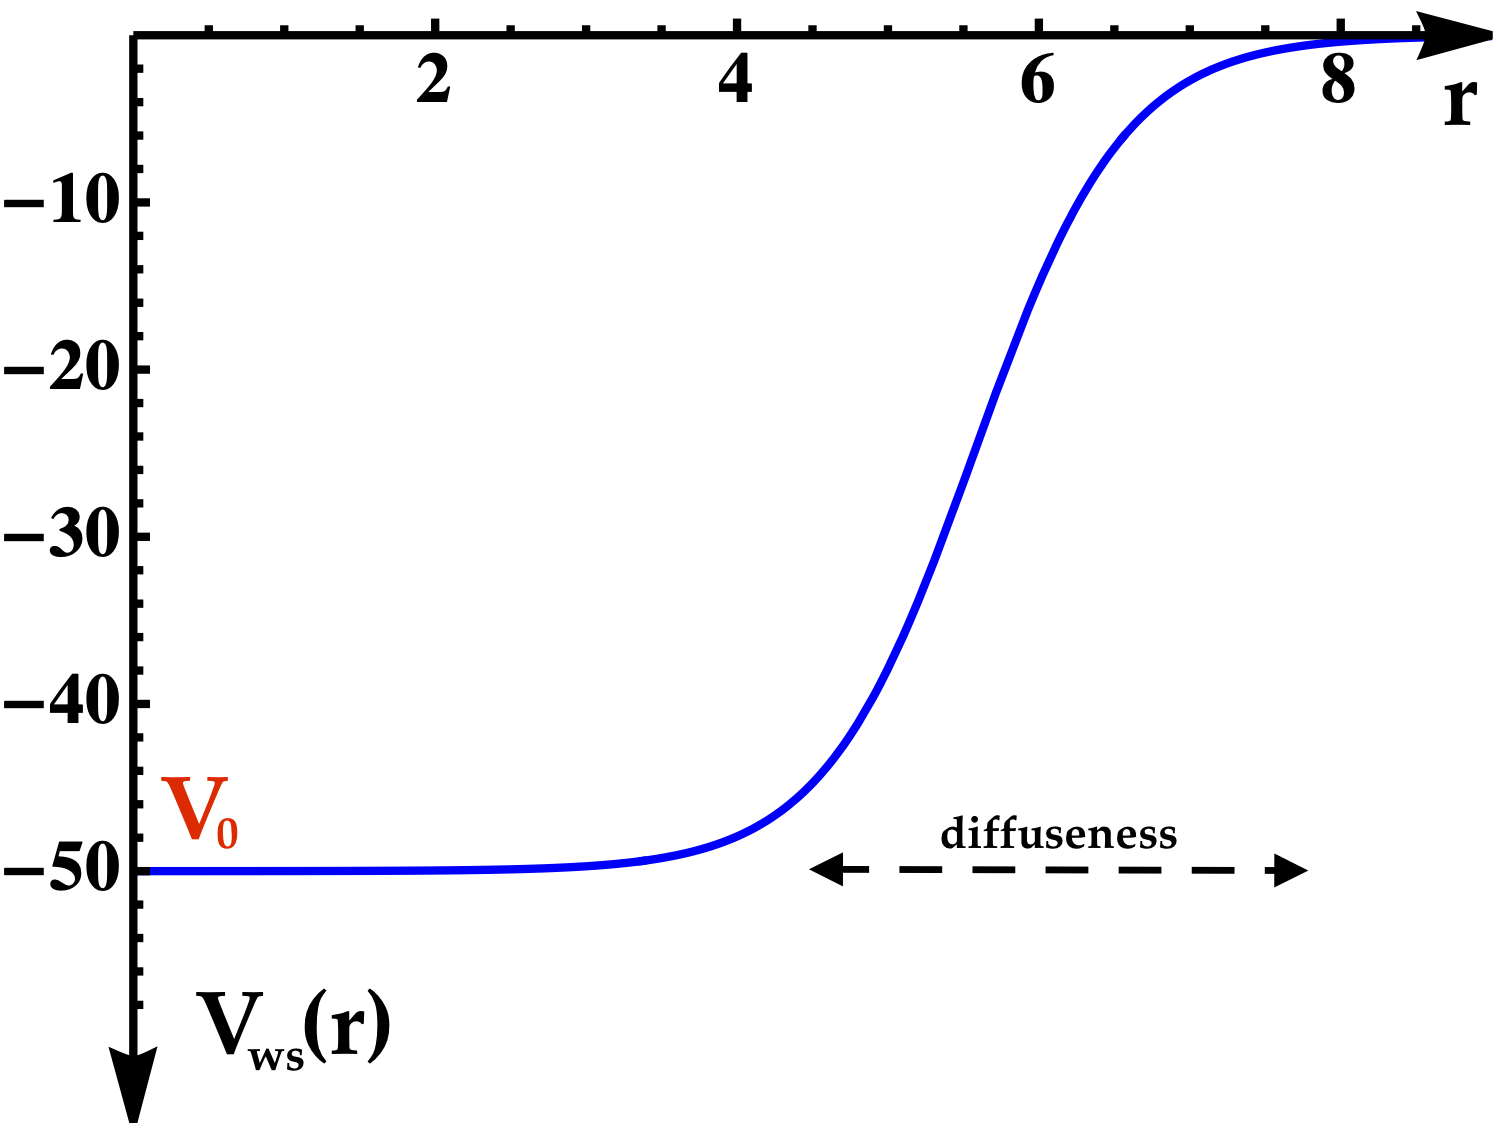
\includegraphics[scale=0.2]{Chapters/Figures/ws_potential_plot.png}
    \caption{The shape of the Woods-Saxon potential, defined by Eq. \ref{woods-saxon-potential}. The parameters are arbitrarily chosen as: $V_0=50$ MeV, $R=5.57$ fm, and $a=0.5$ fm.}
    \label{woods-saxon-plot}
\end{figure}

Fig. \ref{woods-saxon-plot} shows the shape of a typical Woods-Saxon potential. Aiming at a final Hamiltonian which describes the motion of the nucleon within the mean-field potential, the formula can be readily obtained:
\begin{align}
    H&=-\frac{\hbar^2}{2m}\nabla^2+V_\text{ws}^\text{central}+(\vec{l}\cdot\vec{s})_\text{term}\ ,\\
    H&=-\frac{\hbar^2}{2m}\nabla^2-\frac{V_0}{1+e^{\frac{r-R_0}{a}}}+A\vec{l}\cdot\vec{s}\ .
\end{align}
In addition to the shape of the Woods-Saxon potential, a comparison between it, a SHO,and the square-well-like potential is made in Fig \ref{shell-model-functional-potentials}.
\begin{figure}
    \centering
    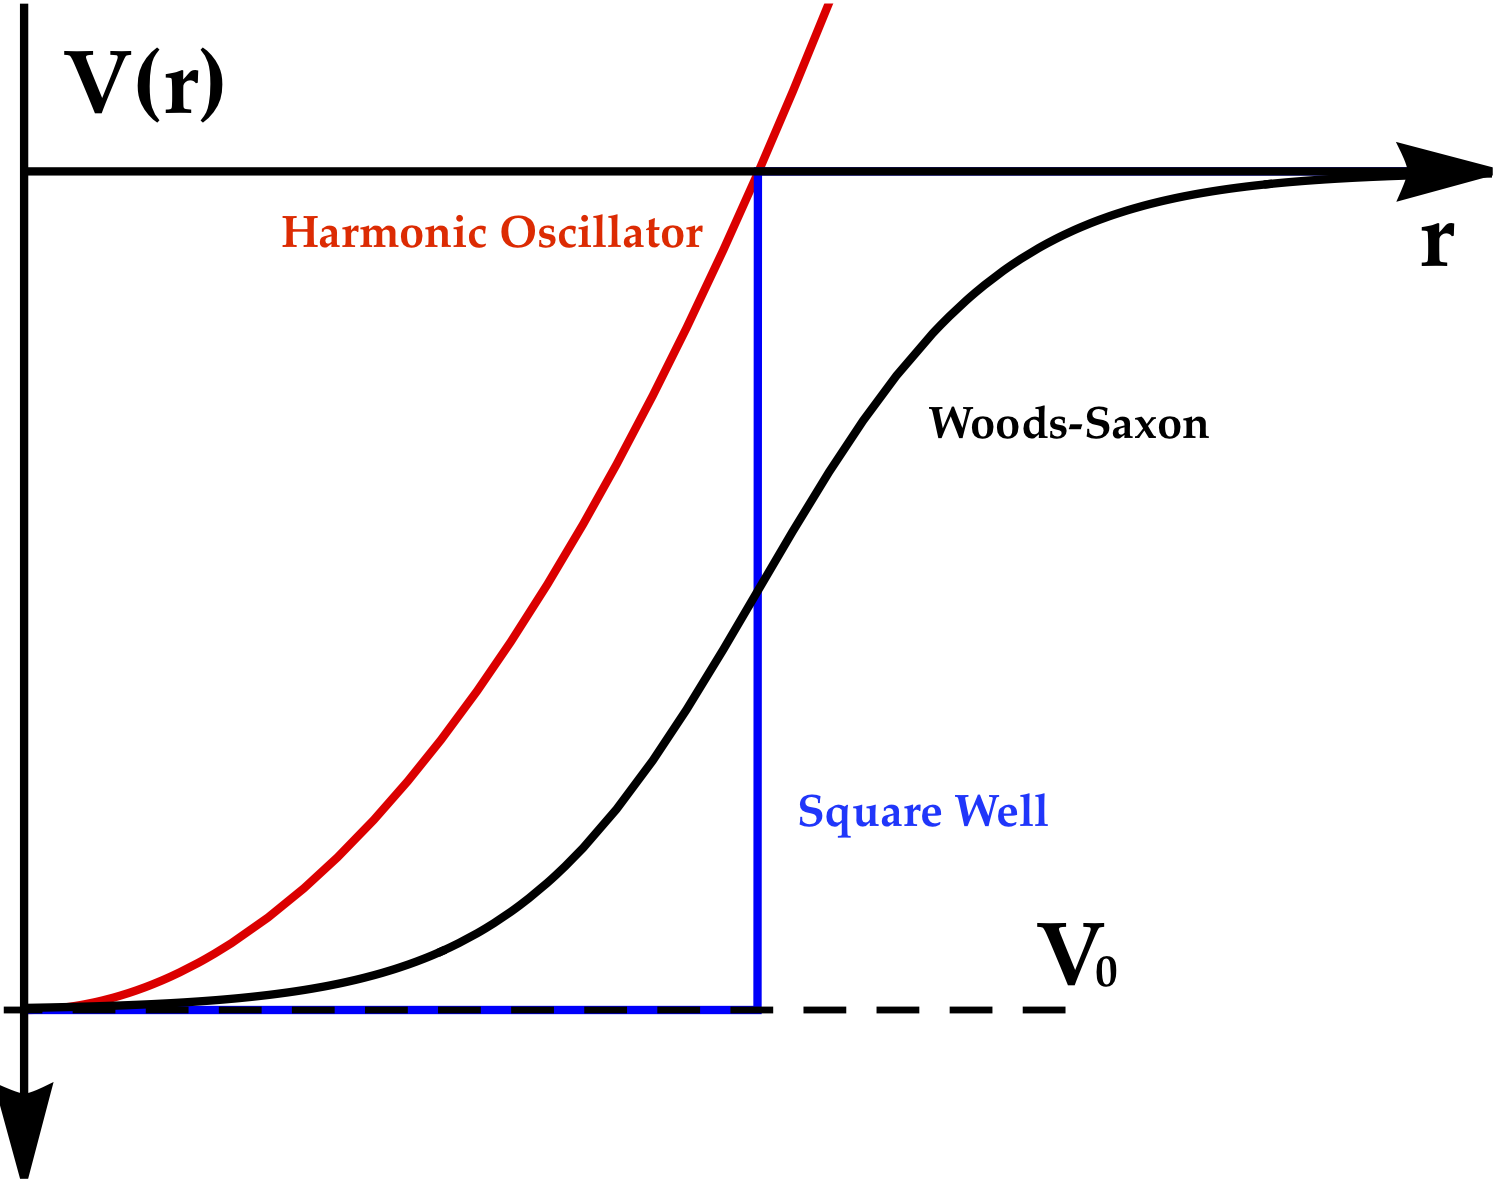
\includegraphics[scale=0.2]{Chapters/Figures/functional-potentials-shell-model.png}
    \caption{A schematic representation with the three kind of potentials used to describe the shell model: harmonic oscillator, Woods-Saxon, and for completeness, the square-well.}
    \label{shell-model-functional-potentials}
\end{figure}

The difference between the pure form of the Woods-Saxon potential and the total potential, where the spin-orbit contribution is amended, can be seen in Fig. \ref{woods-saxon-energy-levels}.
\begin{figure}
    \centering
    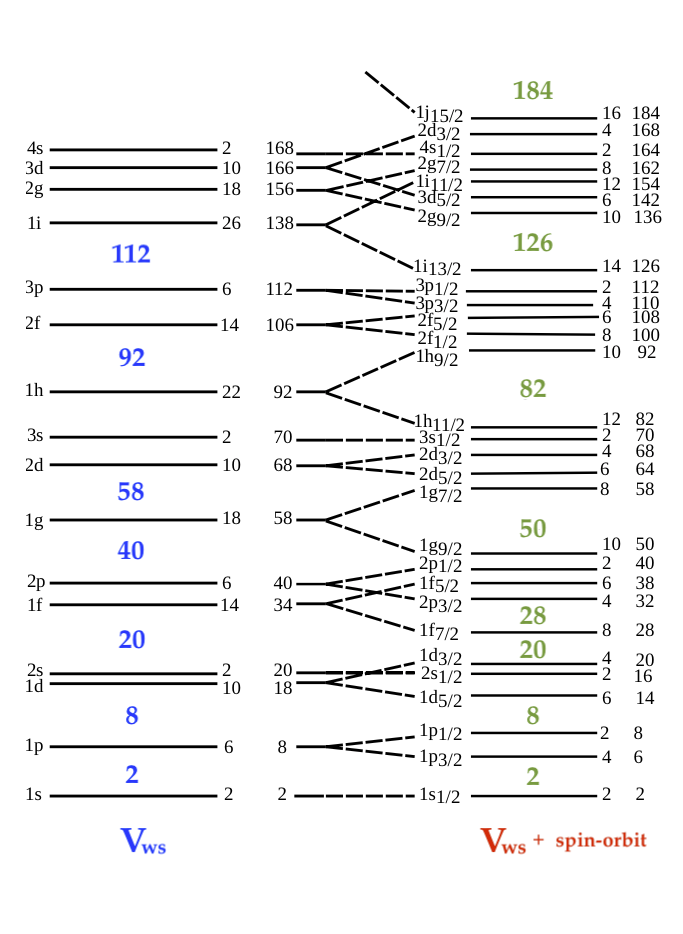
\includegraphics[scale=0.46]{Chapters/Figures/energy_levels_WS.png}
    \caption{The left side represents the energy levels calculated for the Woods-Saxon potential given by Eq. \ref{woods-saxon-potential}, and the right side shows the single-particle energies with the spin-orbit correction added, as in Eq. \ref{woods-saxon-so-potential}. Figure adapted from Ref. \cite{lewis2019lifetime}.}
    \label{woods-saxon-energy-levels}
\end{figure}

So far, the general discussion concerning the nuclear models was for the case where each nucleon is treated as an \emph{independent} particle moving in an average potential (mean-field potential) which represents an \emph{effective} interaction of all the other nucleons with the nucleon under study. However, such an assumption is not accurate enough (especially for the nuclei that lie far away from the closed shells), and this problem should be treated within a \emph{many-body} approach: considering the mutual interaction between the nucleons. These interactions are also called \emph{residual interactions} \cite{casten2000nuclear,bertulani2007nuclear}. With these residual interactions, an accurate depiction of the nucleus might be achieved, and in the following sections, the \emph{Deformed Shell Model} will be employed, reaching to the famous Nilsson model/theory of describing the nucleus.

\section{Deformed Shell Model}

In the previous section, the discussion was focused on an approximate description of the (independent) motion of a nucleon within an average potential. That potential is generated by the interaction of that nucleon with all the remaining nucleons within the compounding nucleus. Indeed, for spherical nuclei, the model described previously works really well and it is a successful tool in reproducing and predicting the properties of nuclear states, especially if the excited states have nucleonic configurations that are dominated by a single nucleon or a very small number of `extra' nucleons.

For nuclei that are even in both the proton number and the neutron number (i.e., even-even nuclei), the nuclear ground-state has a spin and parity that are properly reproduced by the \emph{spherical shell model}: $I^\pi=0^+$. In a nucleus with complete shells, the \emph{net spin} must be zero while for the nucleus with one nucleon missing from a complete shell closure (a hole), that ground-state spin should equal to the total a.m. $j$ value of the orbital which that particular hole is occupying. Moreover, the parity of the ground-state for a given nucleus is determined by the orbital a.m. value $l$:
\begin{align}\pi=(-)^l\to
    \begin{cases}
        +1 &\text{for even-}l\ \text{levels}\\
        -1 &\text{for odd-}l\ \text{levels}\\
   \end{cases}\ .
\end{align}
For odd-odd nuclei, one can find the ground-state (g.s.) spin and parity via the coupling of the spin and parity of the last two valence nucleons \cite{krane1991introductory,bertulani2007nuclear}. The coupling rules that are allowed in the odd-odd nucleus were determined more than 50 years ago by Gallagher et al. \cite{gallagher1958coupling}:
\begin{align}
    I&=j_p+j_n\ \text{if}\ j_p=l_p\pm\frac{1}{2}\ \text{and}\ j_n=l_n\pm\frac{1}{2}\ ,\\
    I&=|j_p-j_n|\ \text{if}\ j_p=l_p\pm\frac{1}{2}\ \text{and}\ j_n=l_n\mp\frac{1}{2}\ .
\end{align}

\subsection{Deformed Shell Model - Nilsson Model}

The idea that some nuclei are deformed in their ground-state was enforced experimentally a long time ago by measuring quantities such as density distributions, nuclear quadrupole moments \cite{casten2000nuclear} and so on. The non-spherical shapes are given by the existence of nucleonic configurations that lie away from the major shell closure. In Chapter \ref{chapter-2} the description of the nuclear shapes was treated, using the well-known formula for the parametrization of the nuclear radius in terms of the collective coordinates (see Eq. \ref{nuclear-shape}), resulting in the known nuclear shapes: \emph{spherical}, \emph{axially-symmetric} (that is prolate or oblate), and \emph{axially-asymmetric} (or triaxial). 

Developed by Nilsson in 1955 \cite{nilsson1955binding} for treating the \emph{deformed nuclei} proved to be a big pillar within the nuclear community, especially for the study of medium and heavy nuclei. In essence, this tools is a modified shell model which allows for deformations to be taken into account by the use of the \emph{anisotropic harmonic oscillator} (AHO). Similarly as for the basic shell model, the goal is to obtain an expression for the single-particle energies of a nucleon. The basic Hamiltonian corresponding to this kind of system is shown below \cite{bertulani2007nuclear}:
\begin{align}
    H=H_0+a_1\vec{l}\cdot\vec{s}+a_2l^2\ ,
    \label{nilsson-simple-hamiltonian}
\end{align}
where $H_0$ is a Hamiltonian for the AHO. The general expression for this kind of oscillator is of the form:
\begin{align}
    H_\text{AHO}\equiv H_0=-\frac{\hbar^2}{2m}\nabla^2+\frac{1}{2}m(\omega_x^2x^2+\omega_y^2y^2+\omega_z^2z^2)\ .
\end{align}
In the general expression of the single-particle Hamiltonian, the constants $a_1$ and $a_2$ are usually determined via adjustments to the experimental results. It can be seen that the centrifugal-like term $l^2$, which simulates a flattening of the oscillator potential, and the $\vec{l}\cdot\vec{s}$ term are still present here, as it was the case for the spherical shell model. However, the explicit form of Eq. \ref{nilsson-simple-hamiltonian} is as follows:
\begin{align}
    H_\text{Nil}=-\frac{\hbar^2}{2m}\nabla^2+&\frac{1}{2}m(\omega_x^2x^2+\omega_y^2y^2+\omega_z^2z^2)-2\kappa\hbar\omega_0(\vec{l}\cdot\vec{s})\nonumber\\&-2\kappa\hbar\omega_0\mu\left(l^2-\langle l^2\rangle_N\right)\ .
    \label{eq-full-nilsson-ham}
\end{align}
Obviously, the parameters $\kappa$ and $\mu$ act as strength parameters for the spin-orbit coupling term and the centrifugal term, respectively. The last term is a correction, which was originally considered as $\mu l^2$, but it was pointed by Gustafson et al. \cite{gustafson1967nuclear} that the shift in energy is way too large for big values of $N$ (principal quantum number). As a result, taking the current expression for the correction term helps to compensate. The three \emph{oscillator frequencies} are chosen to be inversely proportional to the semi-axis lengths of the deformed ellipsoid (denoted by $a_x$, $a_y$, and $a_z$) such that:
\begin{align}
    \omega_r=\omega_0\frac{R_0}{a_r}\ ,\ r=x,y,z\ .
\end{align}
For the spherical case, the oscillator frequency $\hbar\omega_0$ is set to $41A^{-1/3}$ MeV (calculation for this value arise from the shell model with SHO \cite{bertulani2007nuclear}). For the axially-symmetric case, one can choose the $z$-axis as symmetry axis, implying that thw oscillator frequencies along the $x$ and $y$ axes are equivalent (that is $\omega_x=\omega_y\equiv\omega_\perp$).

Following the calculations done in \cite{bertulani2007nuclear}, one can express the two relevant oscillator frequencies in terms of a deformation parameter $\epsilon_2$ (whose dependence on the quadrupole deformation parameter $\beta_2$ has been shown in Eq. \ref{epsilon-beta-relation}) as such:
\begin{align}
    \omega_\perp^2=\omega_0^2\left(1+\frac{2}{3}\epsilon_2\right)\ ,\\
    \omega_z^2=\omega_0^2\left(1-\frac{4}{3}\epsilon_2\right)\ .
    \label{oscillator-frequencies-nilsson}
\end{align}
Moreover, a dependence on the deformation parameter itself is employed for the frequency $\omega_0$ that appears in the expressions for $\omega_\perp$ and $\omega_z$, respectively:
\begin{align}
    \omega_0=\left(1-\frac{4}{3}\epsilon_2^2-\frac{16}{27}\epsilon_2^3\right)^{-1/6}\ ,
    \label{omega-0-oscillator-frequency}
\end{align}
where $\bar{\omega}_0$ can be considered a constant written as $\bar{\omega}_0=(\omega_x\omega_y\omega_z)^{1/3}=\text{const}$ (coming from the harmonic oscillator at zero deformation and also considering the conservation of the nuclear volume).

The energy eigenvalues $\epsilon_q$ for the nucleonic state $\psi_q$ belonging to a deformed nucleus can be determined within the Nilsson model by solving the Schrödinger equation associated to each nucleon in particular:
\begin{align}
    H_\text{Nil}\psi_q=\epsilon_q\psi_q\ ,
    \label{nilsson-schrodiner-equation}
\end{align}
where the index $q$ denotes a set with all the relevant quantum numbers. This set is also called the \emph{asymptotic quantum numbers}, and they are used to specify a \emph{Nilsson orbital}. The well-known notation is as follows (still considering the $z$-axis as the symmetry axis):
\begin{align}
    \Omega^\pi\left[Nn_z\Lambda\right]\ .
    \label{nilsson-notation}
\end{align}
\begin{itemize}
    \item $\Lambda$ is the projection of the particle's orbital a.m. along the symmetry axis (component of $l$ along $z$)
    \item $N$ the principal quantum number of the major shell. It also determines the parity as $\pi=(-1)^N$, making the notation from Eq. \ref{nilsson-notation} somewhat redundant in terms of explicitly specifying it
    \item $n_z$ is the number of oscillator quanta along the symmetry axis. More precisely, it gives the number of nodes for the wave-function of that particle along the direction of the $z$-axis
    \item $\Omega$ is the projection of the particle's total a.m. along the symmetry axis (i.e., $\mathbf{j}$). Moreover, the projection of the intrinsic spin of a nucleon onto the symmetry axis can have the values $\Sigma=\pm\frac{1}{2}$, so that $\Omega=\Lambda+\Sigma=\pm\frac{1}{2}$.
\end{itemize}

Fig. \ref{fig-nilsson-quantum-numbers} shows the geometrical meaning of the asymptotic quantum numbers for the Nilsson model. Indeed, for a single nucleon orbiting a deformed core, the vector $\mathbf{R}$ represents the angular momentum of a \emph{rotating nucleus} (having a collective character, since it emphasizes the motion of the nucleus as a whole), the vector $\mathbf{I}$ represents the total a.m. of the entire nucleus, $\mathbf{j}$ is the total a.m. of the single-particle (that is $\mathbf{j}=\mathbf{j}+\mathbf{s}$). However, two more quantum numbers should be mentioned: the projection of the total a.m. $\mathbf{I}$ onto the symmetry axis, denoted by $K$, and the projection of the same vector onto the laboratory axis, referred to as $M$.

\begin{figure}
    \centering
    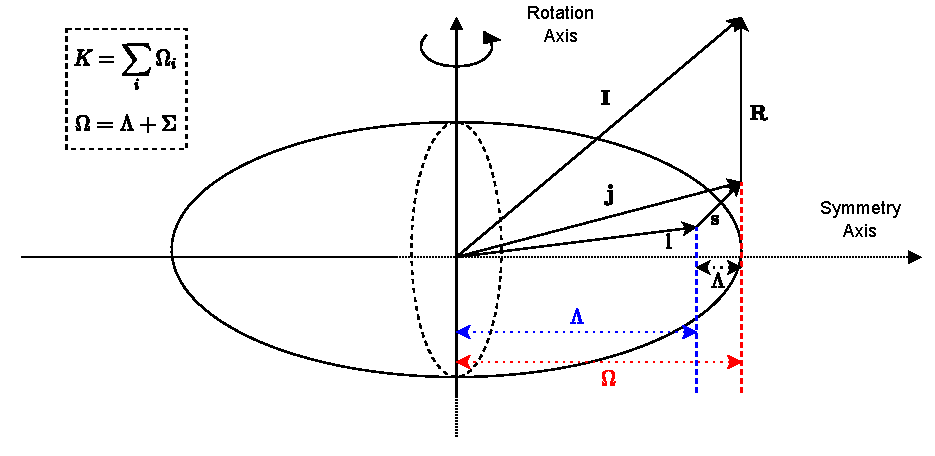
\includegraphics[scale=1]{Chapters/Figures/nilsson_quantum_numbers.pdf}
    \caption{A schematic drawing that shows the geometrical interpretation of the Nilsson asymptotic quantum numbers (see text). This figure is inspired from Ref. \cite{garnsworthy2007neutron}}
    \label{fig-nilsson-quantum-numbers}
\end{figure}

Regarding the quantum numbers sketched in Fig. \ref{fig-nilsson-quantum-numbers}, there is an important aspect which needs to be specified about the two projections $K$ and $\Omega$, respectively, since it would make the understanding of the orbital motion of nucleons more concise. Indeed, it is clear that compared to the spherical case, where different orientations are irrelevant to the energy spectrum of nucleons, here in the deformed case, different directions in space lead to different energies. The orientation is in fact specified by the \emph{magnetic sub-state} of the nucleon, i.e., the projection of the total angular momentum on the symmetry axis. This projections is denoted by $\Omega$ for the single-particle, however, because the rotational angular momentum $\mathbf{R}$ in the axially deformed is perpendicular to the symmetry axis for low-lying states, then it will have no contribution to $K$, meaning that one can use $\Omega$ and $K$ interchangeably.

\subsection{Single-particle states in deformed nuclei}

It is instructive to go into detail about the quantum numbers defined in Eq. \ref{nilsson-notation} since the orbits which characterize the nucleons with such numbers help to point out the nature of nuclear deformations that take place.

The quantum numbers $N$, $n_z$ and $\Lambda$ are good quantum numbers only when the nuclear deformation is large, meaning that $\epsilon$ (or equivalently $\beta$) tends to infinity: also the reason why they are called asymptotic quantum numbers. However, the numbers $\Omega$ and $\pi$ remain good quantum numbers even for low and moderate deformations for the nucleus. It should be noted that if $N$ is even, then $(\Lambda+n_z)$ is also even. Similarly, if $N$ is odd, then the sum of the other two quantum numbers must also be odd \cite{casten2000nuclear}.

Since the eigenvalues of the Hamiltonian $H_\text{Nil}$ ultimately depend on the deformation parameter $\epsilon$, each nucleon will have an orbit (energy) that is deformation dependent. At no deformation (i.e., the spherical case), all the energy levels for a single-particle state will have a $2j+1$ degeneracy. This translates to the fact that all $2j+1$ possible orientations of $\vec{j}$ are equivalent, when referring to any arbitrary axis of choice. On the other side, when the potential is deformed, this will no longer hold: the energy levels in the deformed potential will depend on the spatial orientation of the orbit itself: the energy depends on the component of $\vec{j}$ along the symmetry axis of the core. 

As an example, a nucleon from the $f_{7/2}$ shell will be considered. This nucleon can have eight possible components for $\vec{j}$, this is the range $\Omega=[-\frac{7}{2},\frac{7}{2}]$. Because of the reflection symmetry for nuclei for either of the two possible directions of the symmetry axis, the positive components of $\Omega$ will have the same energy as the negative ones: leading to a degeneracy of the levels. Now, the single-particle $f_{7/2}$ state will split up into four new states when deformation emerges: $\Omega=\frac{1}{2},\frac{3}{2},\frac{5}{2},\frac{7}{2}$ and all have negative parity. In Fig. \ref{nillson-orbits-prolate-projections} an illustration with the different orbits of the odd particle is given, for both the prolate deformed nuclei as well as for oblate ones. Similarly, the orbits of the same state are pictorially represented in Fig. \ref{nillson-orbits-oblate-projections}.

\begin{figure}
    \centering
    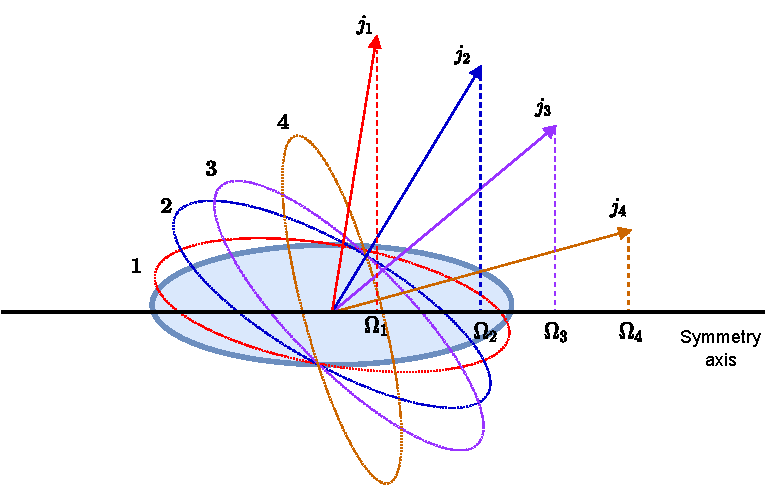
\includegraphics[scale=1]{Chapters/Figures/nillson_SP_orbits.pdf}
    \caption{A simple sketch showing the single-particle orbits for the $j=7/2$ nucleonic state, along the symmetry axis for a \emph{prolate} deformation. The actual projections are $\Omega_1=\frac{1}{2}$, $\Omega_2=\frac{3}{2}$, $\Omega_3=\frac{5}{2}$, and $\Omega_4=\frac{7}{2}$. The figure was inspired from Ref. \cite{krane1991introductory}.}
    \label{nillson-orbits-prolate-projections}
\end{figure}

\begin{figure}
    \centering
    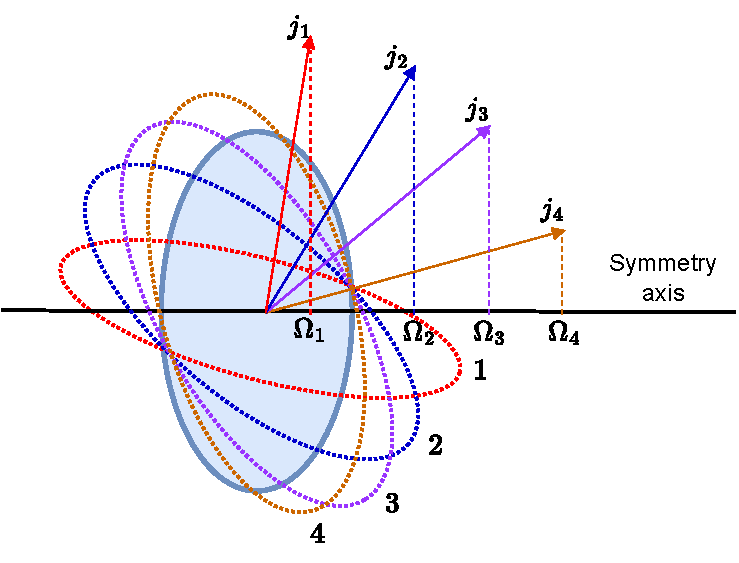
\includegraphics[scale=1]{Chapters/Figures/nillson_SP_orbits_2.pdf}
    \caption{A simple sketch showing the single-particle orbits for the $j=7/2$ nucleonic state, along the symmetry axis for a \emph{oblate} deformation. The actual projections are $\Omega_1=\frac{1}{2}$, $\Omega_2=\frac{3}{2}$, $\Omega_3=\frac{5}{2}$, and $\Omega_4=\frac{7}{2}$. The figure was inspired from Ref. \cite{krane1991introductory}.}
    \label{nillson-orbits-oblate-projections}
\end{figure}

From Figs. \ref{nillson-orbits-prolate-projections} - \ref{nillson-orbits-oblate-projections}, it can be seen that the first orbit (denoted by orbit $1$) lies closest to the core in the prolate case, while in the oblate case this is true for orbit $4$. This plays the role in the interaction strength, meaning that for the prolate case, the orbit $1$ will interact the strongest with the \emph{core}, while in the oblate case, it is the orbit $4$ which has the strongest interaction with the bulk core. Moreover, the strength of interaction indicates the magnitude of the energies for each projection: the stronger the interaction between the orbit and the core, the more tightly bound these states are and lie lower in energy. For prolate deformations, the orbits with smallest $\Omega$ `prefer' to lie lower in energy (interacting strongly with the core). For oblate deformations, the situation is opposite: orbits with the maximal $\Omega$ have the strongest core interactions and therefore lie lowest in energy.

Another way of looking at the coupling of the single-particle with the bulk core can be given in terms of overlaps of their corresponding wave-functions (eigenstates). Indeed, a nucleon lying in the lowest $\Omega$ orbit will have a \emph{maximum} wave-function overlap with a prolate core. On the other hand, nucleons lying in the highest $\Omega$ orbits will have maximum overlap of the wave-function with an oblate core. The overlap gives the overall binding energy between the two systems (i.e., core and particle) as explained in the previous paragraph. Discussion about the wave-function overlap and the nuclear density distribution \cite{frauendorf2014transverse, das2018nuclear} will be made in the following chapters.

The induced degeneracy due to deformation for a particle state $l_j$ is shown in Fig. \ref{nillson-orbits-splittings}, for the same example of the nucleon with the orbit $f_{7/2}$.

\begin{figure}
    \centering
    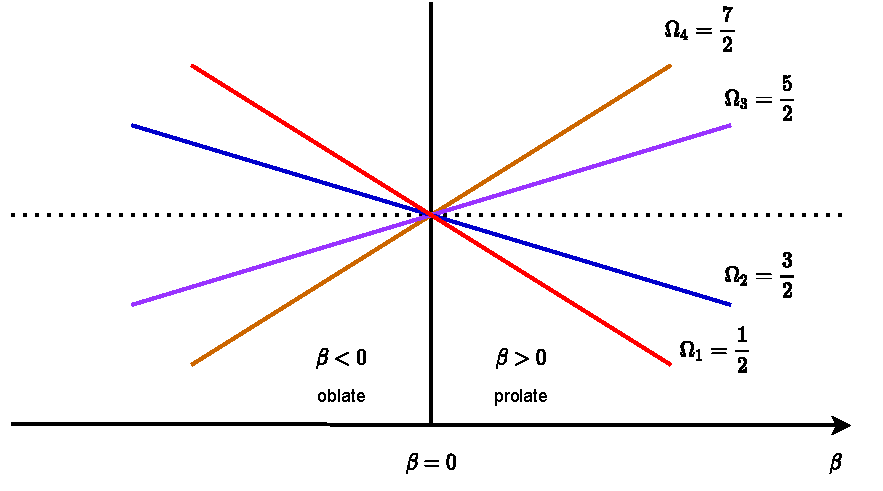
\includegraphics[scale=0.95]{Chapters/Figures/nillson_SP_splittings.pdf}
    \caption{The effect of deformation for the particle state $f_{7/2}$. It can be seen that indeed, as it was mentioned within the text, $\Omega_1$ component lies lowest in energy for the oblate deformation, and $\Omega_4$ component lies the lowest in energy for an oblate deformation.}
    \label{nillson-orbits-splittings}
\end{figure}

Obviously, the sketch shown in Fig. \ref{nillson-orbits-splittings} is just an instructive example, and it does not represent an accurate description of the single-particle energies for deformed nuclei. In fact, if the potential is deformed, the quantum numbers $l$ and $j$ are not valid anymore (that is, the angular momentum is no longer a constant of motion for non-spherical potentials). A proper description of the single-particle orbits are represented by the so-called \emph{Nilsson diagrams}, where the energy for each state is represented as a function of the deformation parameter. Remember that the energies are in fact the eigenvalues of the Schrödinger equation associated to the initial Nilsson deformed Hamiltonian (see Eq. \ref{nilsson-schrodiner-equation}).

The spectrum of one-particle orbits plays an invaluable role within the nuclear structure and the study of deformed nuclei: the picture of one-particle motion in deformed potential works for deformed nuclei much better than the case of single-particle motion in spherical potentials for spherically shaped nuclei. Multiple quantitative analyses have been performed on experimental data of well-deformed (especially odd-$A$) nuclei, from light ($^{25}$Mg, $^{25}$Al) to heavy ($^{169}$Tm, $^{175}$Yb, $^{177}$Yb) \cite{hamamoto2016interplay}. Examples with this kind of diagrams are shown in Figs. \ref{nillson-diagram} - \ref{nillson-diagram-2}. 

\begin{figure}
    \centering
    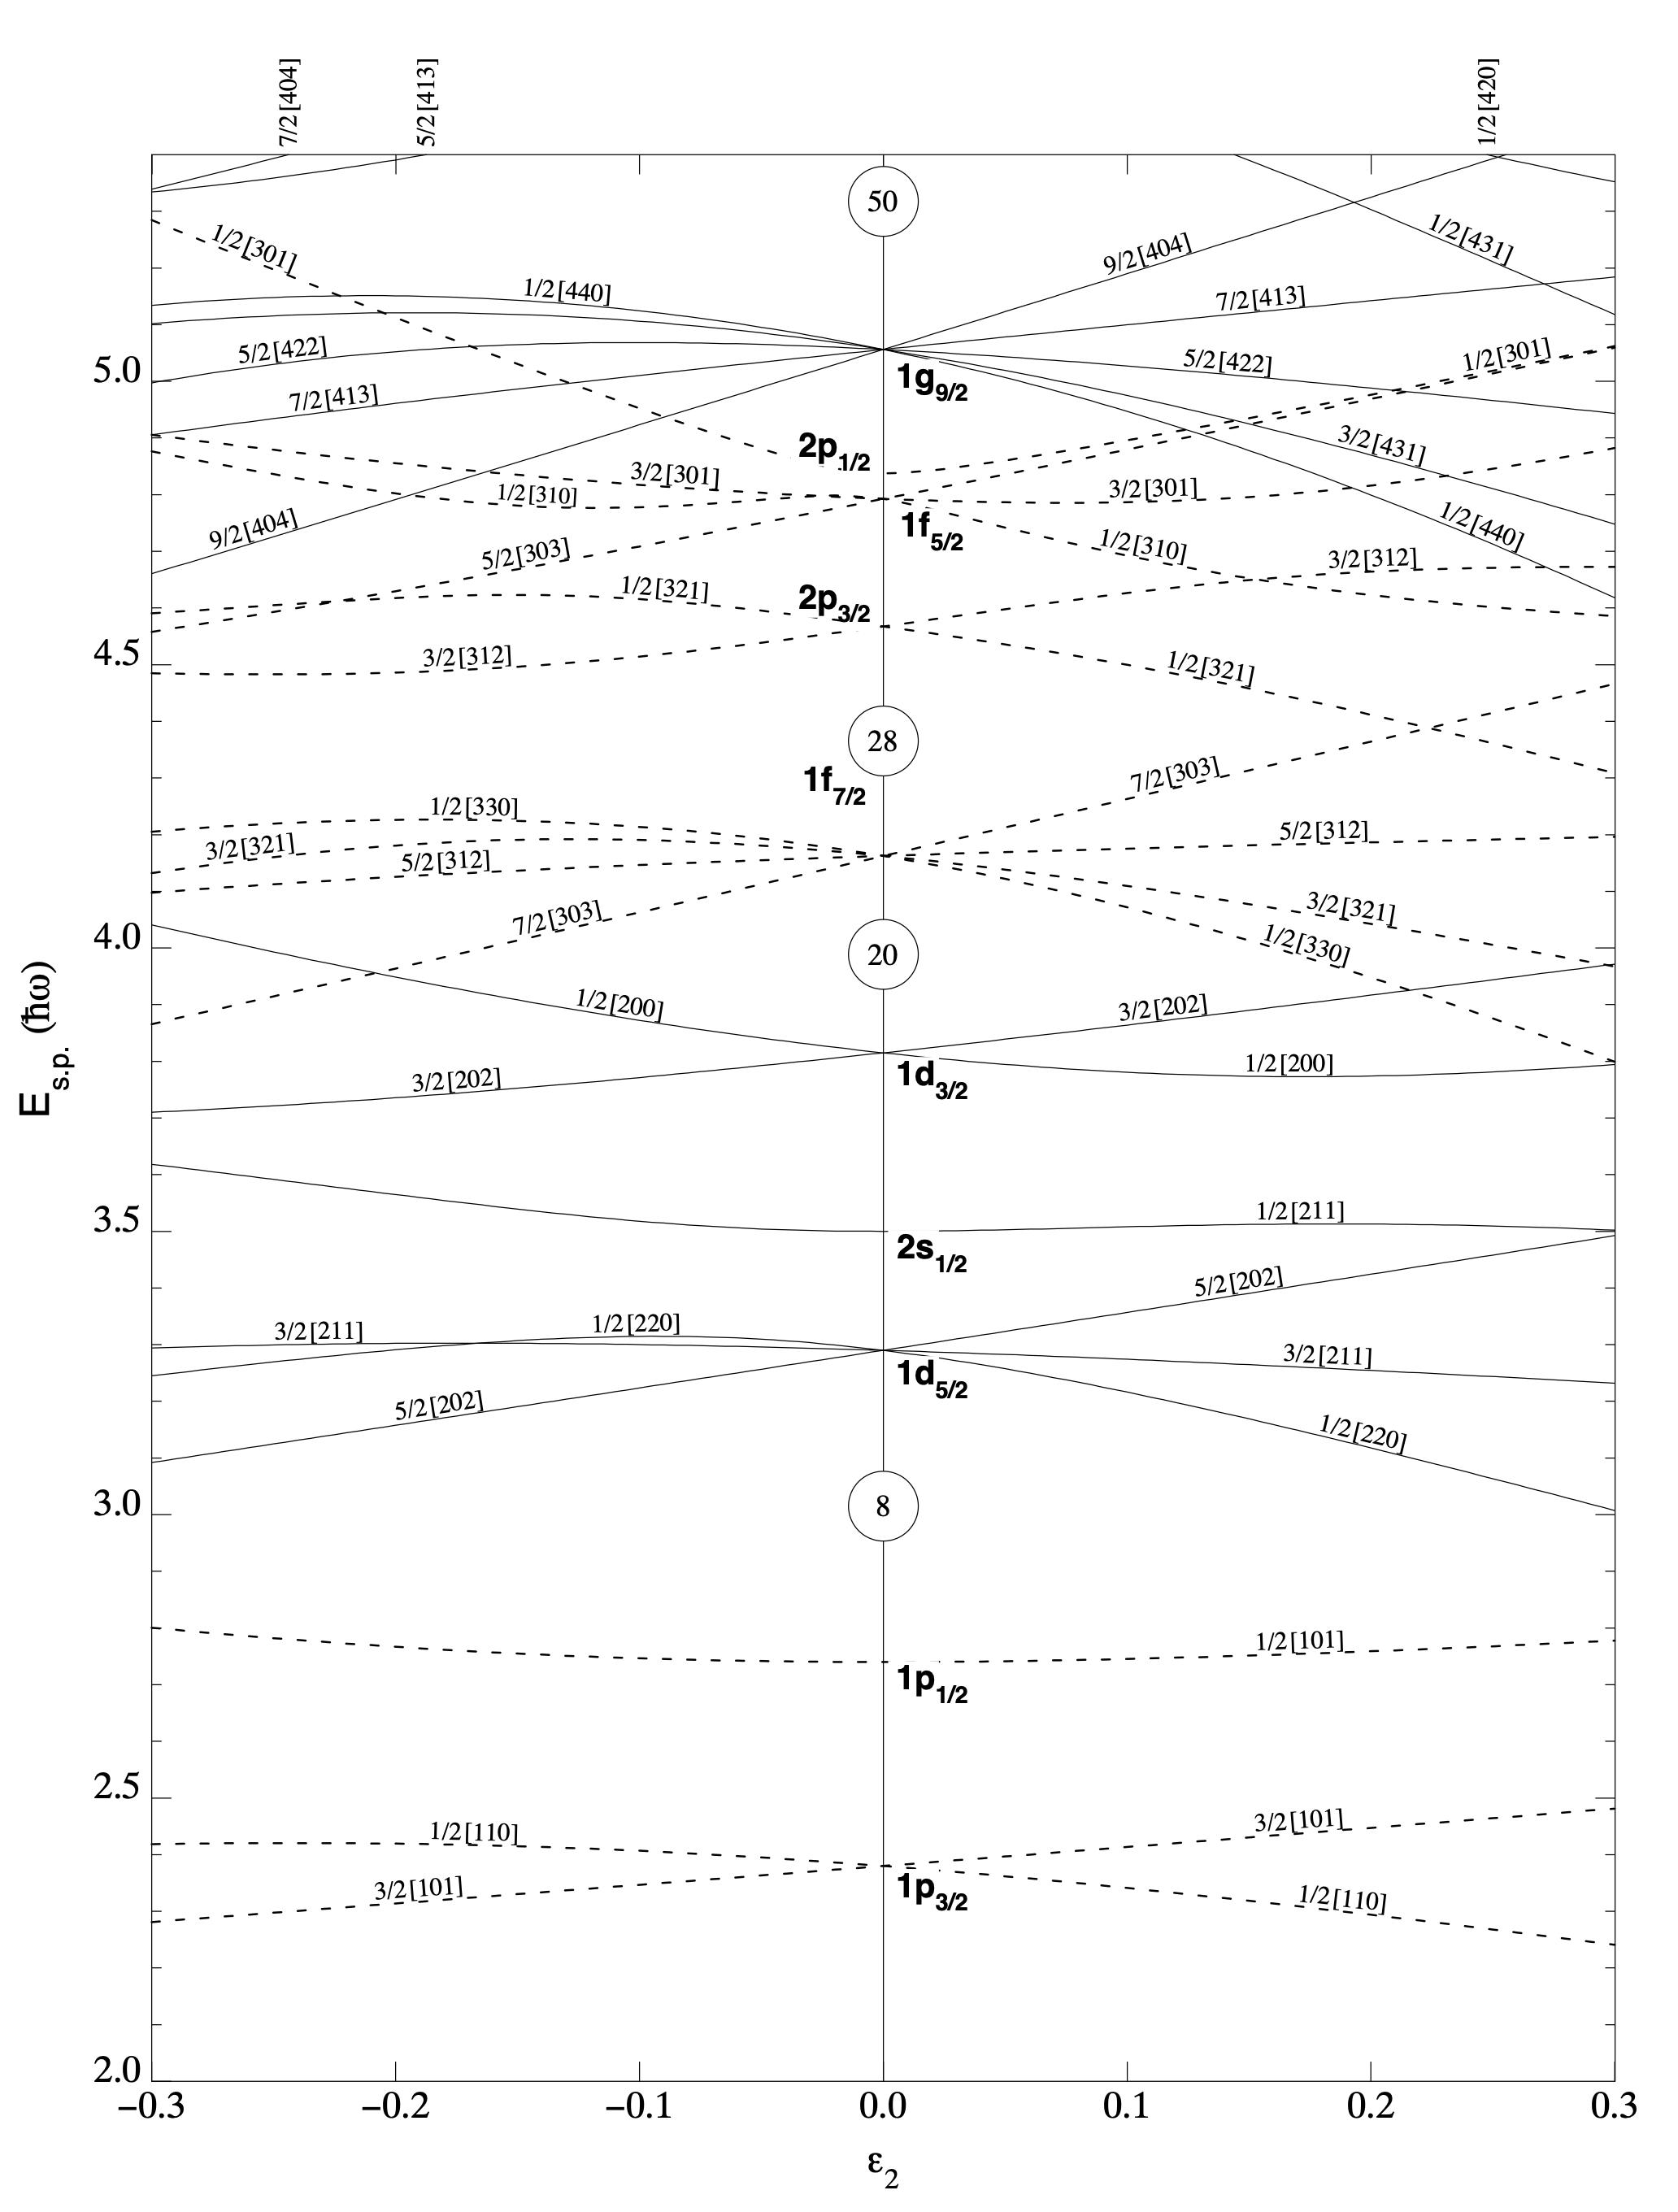
\includegraphics[scale=0.185]{Chapters/Figures/nillson_diagram.png}
    \caption{A Nilsson diagram for protons or neutrons, with $Z$ or $N\leq50$. Picture reproduced from Ref. \cite{ragnarsson2005shapes}.}
    \label{nillson-diagram}
\end{figure}

\begin{figure}
    \centering
    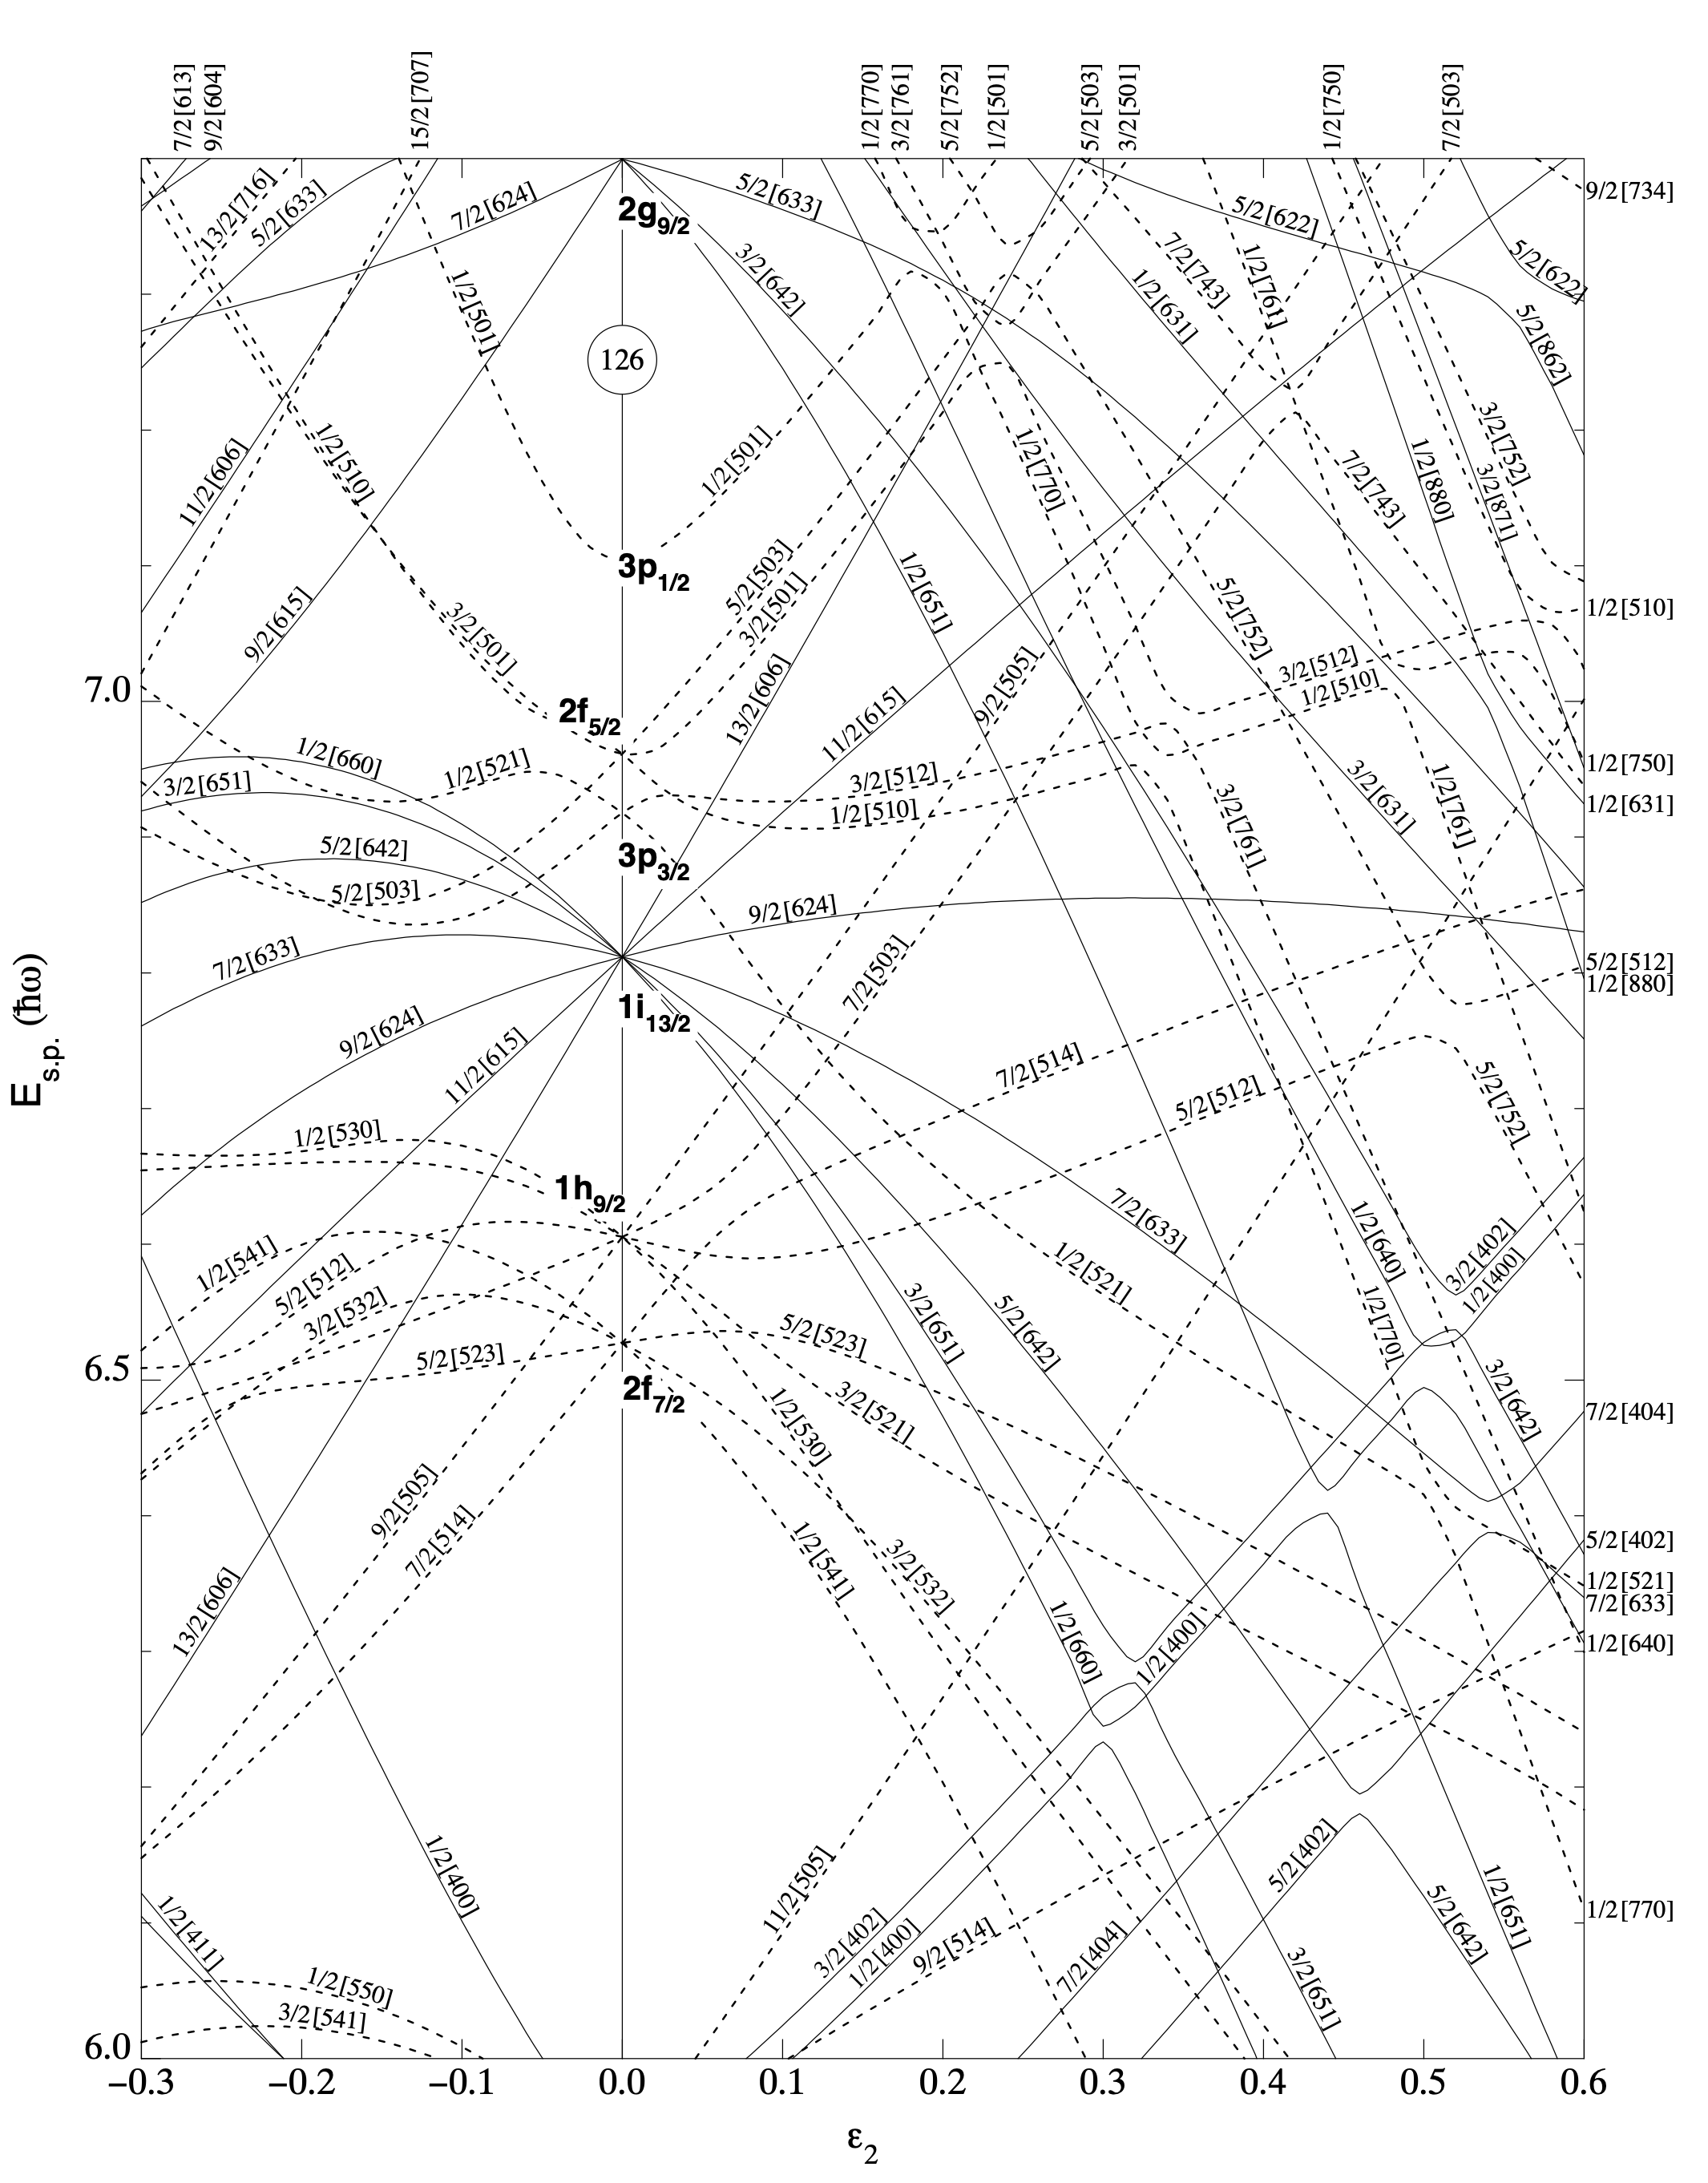
\includegraphics[scale=0.185]{Chapters/Figures/nillson_diagram_2.png}
    \caption{A Nilsson diagram for neutrons, with $82\leq N\leq126$. %This diagram also shows the orbits of neutrons from nuclei such as the Lu isotopes which will be studied in this work.
    Picture reproduced from Ref. \cite{ragnarsson2005shapes}.}
    \label{nillson-diagram-2}
\end{figure}

It can be seen that each state within a Nilsson diagram is represented as a solid line or a dashed line, depending on its parity (remember that the parity quantum number is given by $(-1)^N$ or, equivalently, by $(-1)^l$). The labelling from the Figs. \ref{nillson-diagram} - \ref{nillson-diagram-2} is consistent with the one defined in the previous subsection.

Another important aspect which can be seen in the Nilsson diagrams (for some orbits) is the `crossing' between states with different quantum numbers. In order to fully understand this concept, it is instructive to go into detail about \emph{two-state mixing}.

\subsubsection*{Two-state mixing}

In the work of Casten \cite{casten2000nuclear}, an analytical approach is given for treating the mixing of two different states (energy levels). It starts from the basic idea of two initial levels, each with its corresponding energy $E_1$ and $E_2$, and their associated wave-functions (denoted here with $\psi_1$ and $\psi_2$). Any interaction between them results in the mixing matrix element $\bra{\psi_1}V_\text{int}\ket{\psi_2}$, where $V_\text{int}$ is the arbitrary interaction between the states. This is sketched in Fig. \ref{two-state-mixing-scheme}.

\begin{figure}
    \centering
    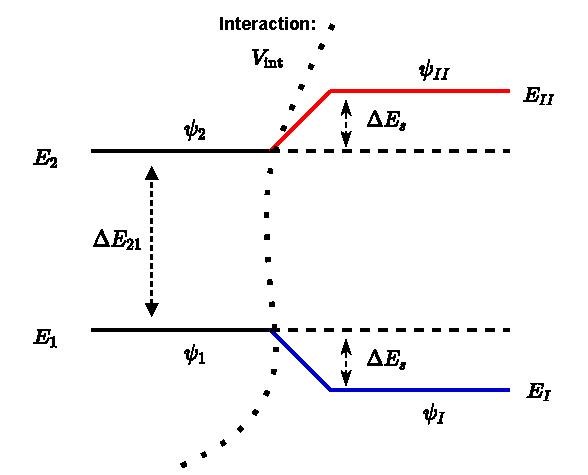
\includegraphics[scale=0.95]{Chapters/Figures/two-state-mixing.pdf}
    \caption{Defining the mixing between two different states, with two corresponding energies and wave-functions. Interaction is illustrated via the curved line and $V_\text{int}$ term.}
    \label{two-state-mixing-scheme}
\end{figure}

This problem can be solved by finding the final energies and wave-functions, this being done via the diagonalization procedure of a $2\times 2$ matrix, where the main diagonal contains the two energies and off-diagonal terms represent the interaction itself. The final states will be denoted here with ($E_I$, $E_{II}$) for the energies and ($\psi_I$, $\psi_{II}$) for the wave-functions. As a general rule, the mixing depends on the initial separation $\Delta E_{21}=(E_2-E_1)$ and the matrix element $\bra{\psi_1}V_\text{int}\ket{\psi_2}$. Given a large spacing, the effect of a given matrix element will be quenched. Moreover, even for a small matrix element, it can introduce a large mixing if the energy separation between the states is small (that is, the unperturbed states are lie close in energy). 

A reduction from these two parameters can be performed, obtaining a single universal mixing expression that is valid for any arbitrary interaction and any initial spacing. As a first step, one should define the ratio between the spacing of the unperturbed states ($Delta E_{21}$) and the strength of the matrix element:
\begin{align}
    R=\frac{\Delta E_{21}}{V_\text{int}}\ .
\end{align}
With this quantity, the newly perturbed energies $E_I$ and $E_{II}$ are readily obtained \cite{casten2000nuclear}:
\begin{align}
    E_I&=\frac{1}{2}(E_1+E_2)+\frac{\Delta E_{21}}{2}\sqrt{1+\frac{4V_\text{int}^2}{\Delta E_{21}^2}}\ ,\\
    E_{II}&=\frac{1}{2}(E_1+E_2)-\frac{\Delta E_{21}}{2}\sqrt{1+\frac{4V_\text{int}^2}{\Delta E_{21}^2}}\ .
    \label{eq-two-state-mixing-energies}
\end{align}

Even more useful would be to find the amount by which each energy is shifted after the interaction. This is denoted in Fig. \ref{two-state-mixing-scheme} by $\Delta E_S$ and its expression depends on $\Delta E_{12}$ as such:
\begin{align}
    |\Delta E_S|=|E_{II}-E_2|=|E_{I}-E_1|=\frac{\Delta E_{21}}{2}\left[\sqrt{1+\frac{4}{R^2}}-1\right]\ .
    \label{eq-shift-mixed-states}
\end{align}
The two perturbed wave functions are as follow:
\begin{align}
    \psi_I&=\alpha\psi_1+\beta\psi_2\ ,\nonumber\\
    \psi_{II}&=-\beta\psi_1+\alpha\psi_2\ ,
\end{align}
where the two amplitudes $\alpha$ and $\beta$ must verify the condition $\alpha^2+\beta^2=1$ and:
\begin{align}
    \beta=\frac{1}{\left\{1+\left[\frac{R}{2}+\sqrt{\frac{R^2}{4}+1}\right]^2\right\}^{1/2}}
    \label{eq-beta-mixing-amplitude}
\end{align}

It is noteworthy to point out that the amplitude $\beta$ is in fact a function that only depends on $R$ (i.e., the ratio between the unperturbed energy splitting and the interaction strength). Similarly, by dividing the shift in energy $\Delta E_S$ to the initial splitting $\Delta E_{21}$, one will obtain an expression that is independent of the initial level spacing:
\begin{align}
    \frac{|\Delta E_S|}{\Delta E_{21}}=\frac{|E_{II}-E_{2}|}{\Delta E_{21}}=\frac{|E_{I}-E_{1}|}{\Delta E_{21}}=\frac{1}{2}\left[\sqrt{1+\frac{4}{R^2}}-1\right]
\end{align}

The importance of these formula will be now emphasized through a numerical example. First of all, the evolution of the ratio of the unperturbed shift and the interaction can be graphically represented as a function of the small mixing amplitude $\beta$ by the use of Eq. \ref{eq-beta-mixing-amplitude}. The graphical representation is shown in Fig. \ref{fig-beta-mixing-amplitude}. Following this analysis, also in Fig. \ref{fig-beta-mixing-amplitude} the shape of $R$ as a function of the energy shift of the perturbed states can be visualized.

\begin{figure}
    \centering
    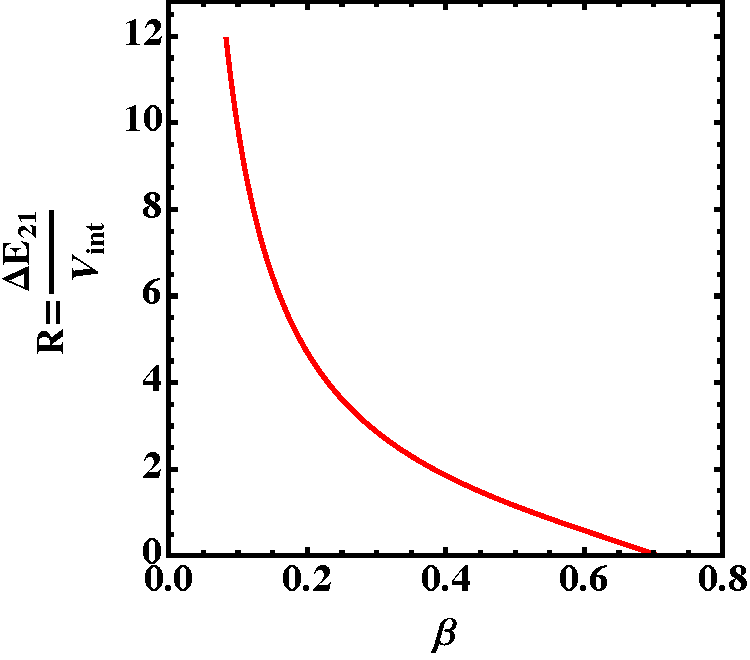
\includegraphics[scale=0.5]{Chapters/Figures/beta_mixing_amplitude.pdf}
    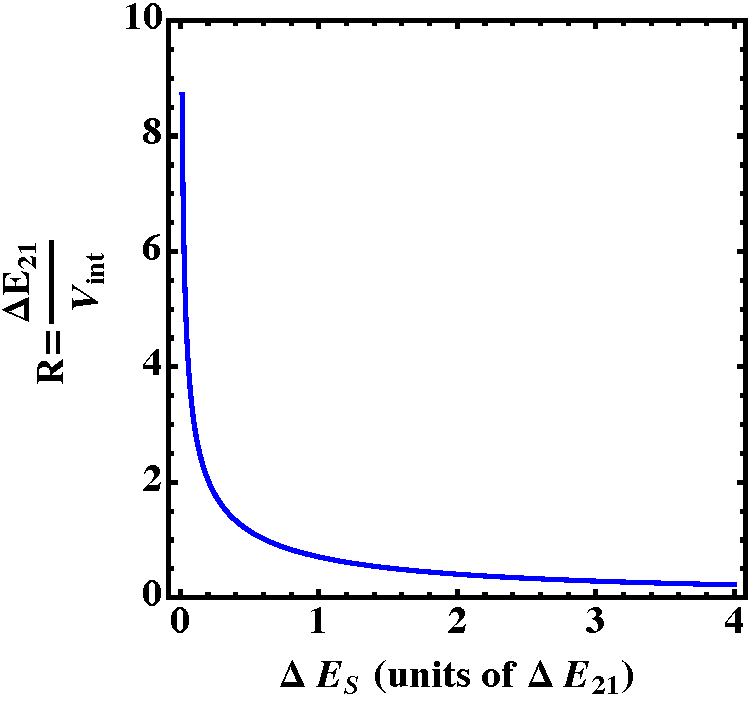
\includegraphics[scale=0.5]{Chapters/Figures/energy_shift_mixing_shape.pdf}
    \caption{\textbf{Left:} The dependence of $R$ (see text) on the mixing amplitude $\beta$. \textbf{Right}: The dependence of $R$ (see text) on the energy shift of the perturbed states ($\Delta E_S$).}
    \label{fig-beta-mixing-amplitude}
\end{figure}

For an arbitrary case where two initial states are separated by, say $\Delta_{21}=0.07$ MeV, and they become \emph{perturbed} via the interaction with a strength $V_\text{int}=0.03$ MeV, this gives a value of $R=3.5$ and, moreover, the mixing amplitude is $beta=0.256$. The two states will both be shifted by only $\Delta E_S=5.31$ keV (accounting for about $7.6 \%$ of the initial separation). Indeed, for this particular example, the perturbation results in an energy shift that is rather small compared to the initial state spacing.

% \begin{figure}
%     \centering
%     \caption{}
%     \label{mixing-energy-shift-shape}
% \end{figure}

Besides the numerical example discussed above, there are also two extremely important limiting situations when two states interact via a perturbation. The first one is the so-called \emph{strong mixing limit}, when the two initial states are degenerate (i.e., there is practically no spacing between them and $\Delta_{21}=0$). In this situation, the analytical expressions from Eq. \ref{eq-shift-mixed-states} fail to provide a quantitative analysis, but from Eq. \ref{eq-two-state-mixing-energies} a small adjustment of the expression will give rise to the following:
\begin{align}
    E_{I,II}=\frac{1}{2}\left[(E_1+E_2)\pm2V_\text{int}\right]=E_0\pm V_\text{int}\ ,
\end{align}
where the initial (common) energy of the two degenerate states is denoted by $E_0$. The above equation indicates the important fact that the energy shift which the two states suffer via the perturbation is only given by the \emph{mixing matrix element}. This means that the final separation energy for a two-state isolated system can never be closer than twice the interaction strength ($2V$). In the degeneracy case, the values for $\beta$ and $\alpha$ are readily obtained: ($\beta=\alpha=\frac{1}{\sqrt{2}}=0.707$), such that the states are completely mixed. Consequently, the mixed wave-functions of two (initially) degenerate states do not depend on the strength $V_\text{int}$ between them. The limiting case of \emph{strong mixing} of two degenerate levels is sketched in Fig. \ref{strong-mixing-fig}.

\begin{figure}
    \centering
    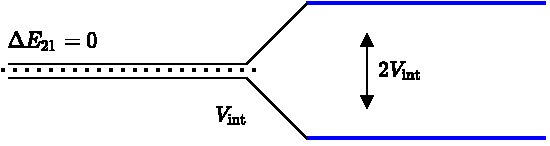
\includegraphics[scale=0.95]{Chapters/Figures/mixing_strong_coupling.pdf}
    \caption{The \emph{strong mixing} limit for two energy levels that are interacting via a perturbation. The initial two levels are degenerate, such that their splitting is null.}
    \label{strong-mixing-fig}
\end{figure}

The second limiting case is called \emph{weak mixing limit}, corresponding to a very large value of $R$ (meaning that the initial separation of the states is very large compared to the magnitude of the interaction itself). The shift in energy of the perturbed states in this case is given by:
\begin{align}
    \frac{|\Delta E_S|}{\Delta E_{21}}=\frac{1}{R^2}\ .
\end{align}

A graphical representation for the weak mixing is shown in Fig. \ref{weak-mixing-fig}.

\begin{figure}
    \centering
    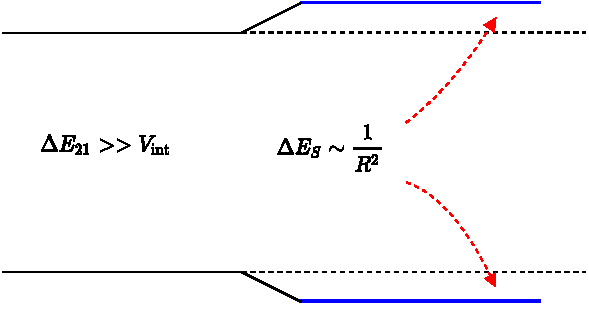
\includegraphics[scale=0.95]{Chapters/Figures/mixing_weak_coupling.pdf}
    \caption{The \emph{weak mixing} limit for two energy levels that are interacting via a perturbation. The interaction strength is much smaller than the initial spacing between states, resulting in a very small energy splitting $\Delta E_{S}$.}
    \label{weak-mixing-fig}
\end{figure}

As a final step in the analysis of the two-state mixing, it is worth mentioning a corner-case which will help to get a better grasp of the Nilsson orbitals. Consider two states (say $\psi_1$ and $\psi_2$) whose energies are parametrized in terms of some argument $c_\text{nuc}$ which is relevant for the nuclear structure of that system (e.g., $c_\text{nuc}$ could be a quadrupole deformation and the two initial states are in fact Nilsson orbits). The remarking `feature' of this hypothesis is that if there indeed exists mixing between the two states, they can never cross each other. The two mixed states will always repel and they can never be closer than twice the mixing matrix element $V_\text{int}$ after mixing occurs. In Fig. the behavior of non-crossing for the mixed states is sketched.
The point at which the two states are the closest to each other represents the case when the wave-functions contain similar admixtures of each of the initial states (unperturbed). The \emph{inflection point} can be seen in Fig. \ref{fig-non-crossing}, where the behavior of the final states $\psi_I$ and $\psi_{II}$ can be seen.

\begin{figure}
    \centering
    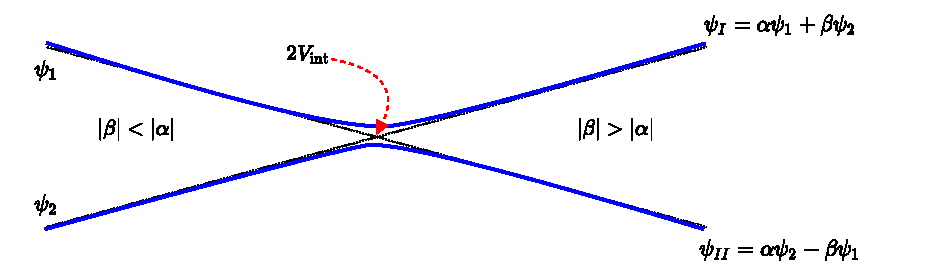
\includegraphics[scale=0.9]{Chapters/Figures/state_non_crossing.pdf}
    \caption{A sketch showing the concept of \emph{non-crossing} between two states. Arrow represents the closest point at which the two states can interaction with each other (i.e., the inflection point).}
    \label{fig-non-crossing}
\end{figure}

\subsection*{Nilsson orbitals}

With the concept of two-state mixing clearly depicted, it is instructive to go further into the Nilsson orbitals and their significance. Recalling Fig. \ref{nillson-orbits-splittings}, the splitting of a $j$ orbital into $j+1/2$ magnetic sub-states can be viewed as a set of orbitals (energies) where the nucleon orbits around the bulk nucleus with an orbit that has a certain \emph{tilt} angle $\theta$ (see the orbits depicted in Figs. \ref{nillson-orbits-prolate-projections} and \ref{nillson-orbits-prolate-projections}). The tilting angle is conceptually showed in Fig. \ref{fig-nilsson-tilting-angle}, where a magnetic sub-state with given $\Omega$ is shown. For that particular orbit, the angle is given by the expression \cite{krane1991introductory,casten2000nuclear}:
\begin{align}
    \sin\theta&=\frac{\Omega}{j}\ , \nonumber\\
    \theta&=\arcsin(\frac{\Omega}{j})\ .
\end{align}
\begin{figure}
    \centering
    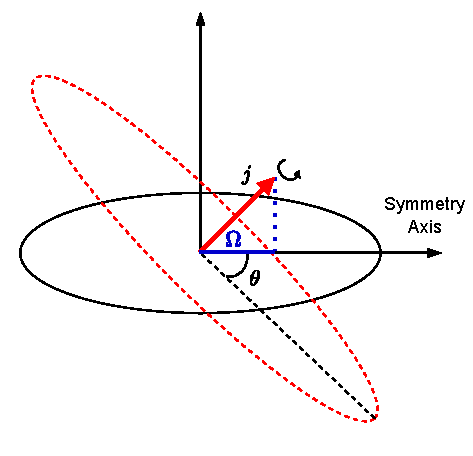
\includegraphics[scale=0.95]{Chapters/Figures/nilsson_tilting_angle.pdf}
    \caption{The orbit of a single particle orbiting the deformed nucleus, defined by the projection of the particle's a.m. $\Omega$ (on the symmetry axis) and the tilting angle $\theta$. Figure inspired from Ref. \cite{casten2000nuclear}}
    \label{fig-nilsson-tilting-angle}
\end{figure}

The change of $\theta$ is rather slow for low $\Omega$ projections, while rapid changes take place at high $\Omega$ values. %It should be noted that this discussion applies to a single-particle total a.m. projection, but as it was discussed previously, using the projection $K$ within calculations is equivalent (since the axially deformed potentials keep $\mathbf{R}$ oriented perpendicular to the symmetry axis).
As a numerical example, the change in $\theta$ is studied for the orbits $j=\{9/2,11/2,13/2\}$, with their corresponding projections. The evolution with $\Omega$ for different orbits can be seen in Fig. \ref{fig-tilting-angle-shape}.

\begin{figure}
    \centering
    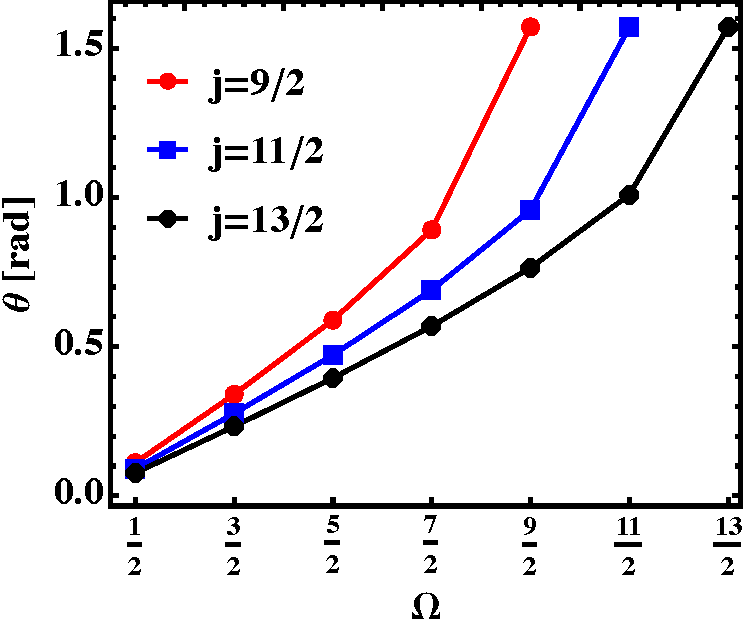
\includegraphics[scale=0.7]{Chapters/Figures/tilted_theta_shape.pdf}
    \caption{The change in $\theta$ with increasing values of $\Omega$, for given orbitals $j$.}
    \label{fig-tilting-angle-shape}
\end{figure}

The simplistic shapes within the splitting of an orbital $j$ into multiple sub-states (see Fig. \ref{nillson-orbits-splittings}) emerge from the considerations regarding the change in tilting angle $\theta$ and the observation that the difference in energy is rather slight (high) depending on low (high) $\Omega$ values.

Based on this discussion, it is clear that a full Nilsson diagrams is constructed with the configuration mixing of different $j$ values, configuration which is superimposed on state-splitting via the $\Omega$ projections. With this idea, one can state that \emph{no two lines in the Nilsson diagram with similar $\Omega$ values can cross each other}. As two such orbits come close to each other, they must repel as shown in Fig. \ref{fig-non-crossing}. Explaining the behavior of the lines that appear in the Nilsson diagrams \ref{nillson-diagram} - \ref{nillson-diagram-2} is straightforward: each line represents a Nilsson state, starting out in a straight line and then sloping downward or upward, depending on the angle of the orbit relative to the bulk nucleus. The \emph{curving} of an orbit starts when it approaches another level with the same quantum number $\Omega$ and parity $\pi$. Thus, the structure of any Nilsson diagram relies on three main features \cite{casten2000nuclear}:
\begin{itemize}
    \item the $\Omega$ splitting
    \item repulsion between two levels
    \item single-particle shell model energies
\end{itemize}

Taking a closer look at the second Nilsson diagram previously shown (see Fig. \ref{nillson-diagram-2}), there are two orbits within the 82-126 neutron shell that can be analyzed in terms of \emph{mixing}: $f_{7/2}$ and $h_{9/2}$. Obviously, the lack of deformation implies a degeneracy of these orbits, but when deformation occurs, splitting kicks in. The angle of the orbital orientation $\theta$ depends on the ratio $\frac{\Omega}{j}$ (recall formula $\theta=\arcsin\frac{\Omega}{j}\approx\frac{\Omega}{j}$ for low $\Omega$). 
Small tilting angles will occur due to i) small values of $\Omega$ or ii) high $j$. As a result, the energies for the orbits $\Omega=1/2,3/2,5/2$ belonging to the $h_{9/2}$ shell are decreasing in energy faster with deformation than those from $f_{7/2}$ orbit. Consequently, the different rates of decrease of the Nilsson energies will overcome any small spherical energy separation $f_{7/2}-h_{9/2}$, making the orbits with low $\Omega$ to approach each other: mixing becoming more pronounced.
But as discussed in the section devoted to \emph{two-state mixing}, two orbits defined by the same quantum numbers cannot cross each other, so the will repel, leading to the \emph{inflection point}. The points can be seen, for example, when looking at the $\Omega=5/2$ and $\Omega=7/2$ orbits, corresponding to $f_{7/2}$ and $h_{9/2}$, respectively.

Lastly, an alternative form of the Nilsson Hamiltonian should be expressed, taking into consideration the already studied nuclear radius (see Eq. \ref{nuclear-shape} which describes the shape of the nuclear surface) and the fact that until now, only the \emph{quadrupole} effects have been relevant to the discussion about deformed potentials in nuclei. Indeed, for quadrupole deformations, the nuclear radius can be simplified to:
\begin{align}
    R(\theta,\varphi)=R_0\left(1+\beta Y_2^0(\theta,\varphi)\right)\ .
    \label{simple-quadrupole-nuclear-surface}
\end{align}

The single-particle Hamiltonian can be written in the general form, starting from the expression Eq. \ref{eq-full-nilsson-ham}:
\begin{align}
    H_\text{Nil}=-\frac{\hbar^2}{2m}+\frac{1}{2}m(\omega_0r)^2-&\frac{4}{3}\sqrt{\frac{\pi}{5}}m(\omega_0r)^2\epsilon Y_2^0(\theta,\varphi)-2\kappa\hbar\omega_0(\vec{l}\cdot\vec{s})\nonumber\\
    &-2\kappa\hbar\omega_0\mu\left(l^2-\langle l^2\rangle_N\right)\ .
    \label{eq-nilsson-ham-spherical-harmonics}
\end{align}

The expression for the oscillator frequencies were already given (defined as functions of the deformation parameter $\epsilon$), and they keep the same form (see Eqs. \ref{oscillator-frequencies-nilsson} - \ref{omega-0-oscillator-frequency}). It is worth mentioning that both forms of $H_\text{Nil}$ are equivalent, and allow to describe the structure of the deformed nuclei in the limits of large deformations (via Eq. \ref{eq-full-nilsson-ham}) and small deformations (via Eq. \ref{eq-nilsson-ham-spherical-harmonics}). Within literature, the two parameters $\kappa$ and $\mu$ have usually values around $0.06$ for the former and $(0\sim 0.7)$ for the latter. As previously shown, the relationship between the $\epsilon$ and $\beta$ deformation parameters is given by $\epsilon=3/4\sqrt{5/\pi}\beta$.

When the deformations are small, $j$ is a good quantum number, and the Eq. \ref{eq-nilsson-ham-spherical-harmonics} represents a Hamiltonian for the AHO (which it was discussed) plus a \emph{perturbation} that is proportional to $\epsilon r^2Y_2^0$. One can consider the eigenstates of the Hamiltonian as some states labelled by the quantum numbers $Nlj$ and $m$ typical to the spherical case. Casten shows that if the angular part $Y_2^0$ is treated as a perturbation, it is possible to obtain a shift in energies relative to $\epsilon=0$ \cite{casten2000nuclear}:
\begin{align}
    \Delta E_{Nljm}=-\frac{4}{3}\sqrt{\frac{\pi}{5}}m\omega_2^0\epsilon\bra{Nljm}r^2Y_2^0\ket{Nljm}\ .
\end{align}

Furthermore, one can perform a separation of the radial and the angular parts while using the known relation for a harmonic oscillator potential:
\begin{align}
    \frac{1}{2}m\omega_0^2\bra{Nljm}r^2\ket{Nljm}=\frac{1}{2}\hbar\omega_0\left(N+\frac{3}{2}\right)\ ,
\end{align}
and, together with the evaluation of the matrix elements for spherical harmonics, the final expression for the energy shift at small deformations is:
\begin{align}
    \Delta E_{Nljm}=-\frac{2}{3}\hbar\omega_0\left(N+\frac{2}{3}\right)\epsilon\frac{\left[3K^2-j(j+1)\right]\left[\frac{3}{4}-j(j+1)\right]}{(2j-1)j(j+1)(2j+1)}\ ,
    \label{nilsson-energy-shifts}
\end{align}
with the projection of the total a.m. on the $z$ axis replacing the projection $m$. Based on Eq. \ref{nilsson-energy-shifts}, the following properties for a Nilsson diagram (within the small deformation regime) emerge:
\begin{itemize}
    \item There is a $K^2$ dependence for the energy shifts
    \item The quadrupole deformation parameter (albeit $\epsilon$ or $\beta$) shows a clear linear dependence for $\Delta E_{Nljm}$
    \item Another linear dependence for the shifts is induced by the principal (oscillator) quantum number $N$.
    \item When the deformation parameter is positive, there are more downward sloping orbits than upward ones. (Example discussed below)
\end{itemize}

For a value of $j$ greater than $1/2$, the terms $\left[3K^2-j(j+1)\right]$ and $3/4-j(j+1)$ are negative, resulting in the following types of orbits: \cite{krane1991introductory}:
\begin{align}
    \text{downward sloping:}&\ K<\sqrt{\frac{j(j+1)}{3}}=\frac{j}{1.8}\approx 0.65j\ ,\\
    \text{upward sloping:}&\ K>0.65j\ .
\end{align}

It was already shown that the angular orientation (i.e., the tilting angle $\theta$) of an orbit is given by $\theta=\arcsin(K/j)$. Checking to see for what value of $\theta$ the ratio $K/j=0.65$ corresponds to, this will lead to $\theta=40^\circ$. Consequently, the physical implication is that any larger \emph{tilt} of an orbit within a prolate quadrupole deformation is energetically unfavorable. In Fig. \ref{fig-nilsson-delta-E-shift} two different $j$ orbits, namely $h_{9/2}$ and $i_{13/2}$ are studied in terms of their energy shifts according to Eq. \ref{nilsson-energy-shifts}. It can be seen that indeed, there are more downward sloping orbitals, since the quadrupole deformation parameter has been set to a positive value $\epsilon=0.22$.

\begin{figure}
    \centering
    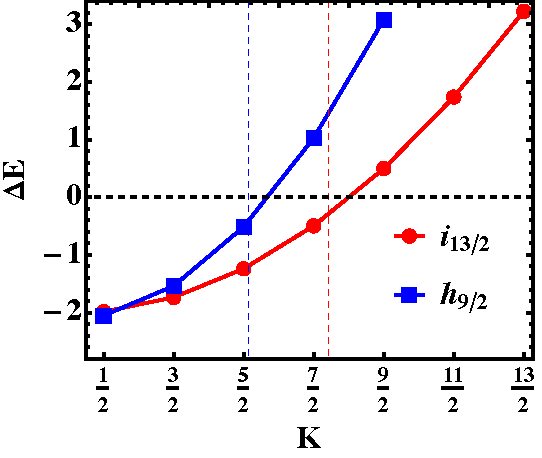
\includegraphics[scale=0.65]{Chapters/Figures/energy_shift_nilssonDeltaE.pdf}
    \caption{The energy shift $\Delta E$ for two orbits: $h_{9/2}$ and $i_{13/2}$ for a given deformation $\epsilon=0.22$. The dashed vertical lines (colored) represent the value for $K$ where the `change' from downward sloping curves to upward sloping curves takes place (that is $K\approx 0.65j$). This is just an illustrative example inspired from the discussion regarding single-particle orbits in Ref. \cite{casten2000nuclear}}
    \label{fig-nilsson-delta-E-shift}
\end{figure}

There is another important physical consequence emerging from the four main characteristics mentioned above, based on the principal quantum number $N$. The dependence on $N$ will imply that the slopes of any Nilsson energy level will be \emph{steeper} as $N$ has large values. As such, heavier nuclei will tend to deform much easier than lighter ones. The explanation for the influence of large $N$ on the steepness was done in Refs. \cite{bohr1998nuclear,krane1991introductory,casten2000nuclear}. Shortly, a nucleon belonging to a high oscillator shell will have a large average radius (the expectation value of $r^2$ was done in Eq. \ref{nilsson-energy-shifts} via the expression $\langle r^2 \rangle=(N+3/2)$ \cite{bertulani2007nuclear}). As the nucleus deforms, the density distribution of the nuclear matter will approach that orbit. The effect on the orbiting nucleon to decrease its energy rapidly as the nuclear matter comes closer to the orbit is due to the \emph{attractive} nature of the nuclear force itself. 
Clearly, this effect is less obvious for a particle in a lower oscillator shell that is already very close to the rest of the nuclear matter.

The centrifugal $\vec{l}^2$ and spin-orbit $\vec{l}\cdot\vec{s}$ terms from Eq. \ref{eq-nilsson-ham-spherical-harmonics} will become negligible in the limit of \emph{large deformation}, such that the Nilsson Hamiltonian will reduce to the known AHO-like form. In this special case, the motion will separate into \emph{independent} oscillations in the direction of the symmetry axis and the perpendicular plane (i.e., in the direction of $z$-axis and $xy$ plane). Consequently, the good quantum numbers for this kind of situation are the $n_z$ and $(n_x+n_y)$ oscillator quantum numbers. Since the eigenvalues for a one-dimensional (and, implicitly for the three-dimensional) harmonic oscillator are established, the energy spectrum for single-particle orbits in the regime of large $\epsilon$ (or, equivalently $\beta$) will be given by:
\begin{align}
    E_{n_x,n_y,n_z}=\hbar\omega_x(N-n_z+1)+\hbar\omega_z\left(n_z+\frac{1}{2}\right)\ .
\end{align}

The remarking feature of the Hamiltonian which corresponds to this set of eigenvalues is its invariance to rotations about the $z$ axis. The projections for the particle's orbital and spin a.m. are constants of motion. As it was previously discussed, the sum of the two projections $\Lambda$ and $\Sigma$ is indeed $\Omega$ or equivalently $K$ in the case of $\vec{R}$ being perpendicular to the $z$-axis.

With this, the description of the Nilsson Deformed Model is clear enough for understanding it and also be able to justify its importance within the rest of the present work. It will be shown that based on the so-called Particle-Rotor-Model \cite{bohr1998nuclear,davydov1958rotational}, it plays a crucial role in determining the Hamiltonians that are specific to the phenomena (and implicitly the nuclei) of interest.

\section{Collective Model}

Although the previous single-particle model is able to successfully treat many nuclei (e.g., those which are lie near closed shells), the single-nucleon motion within a (deformed) potential is not enough to describe for example: nuclear fission, values for quadrupole moments of multiple deformed nuclei \cite{townes1949nuclear} or lifetime measurements that through single-particle calculations fail to reproduce experimental data on some gamma-ray transitions (of electric quadrupole type) \cite{goldhaber1951classification}.

The collective model is one of the most `complete' tools in describing the nuclear phenomena across the chart of nuclides. It brought tremendous progress within nuclear community in order to validate but also predict nuclear behavior in the high-spin limit for example. A major feature of this model is the introduction of the so-called \emph{rotational bands}, characteristic of deformed nuclei which will be discussed in detail later on, since it is of crucial interest to this work.

Developed by Bohr and Mottelson \cite{bohr1953collective,bohr1998nuclear} more than 50 years ago the Nuclear Collective Model, it is based on the Liquid-Drop-Model (which formulated by Niels Bohr \cite{bohr1936neutron}). Moreover, the predictions for nuclear deformation made by Rainwater \cite{rainwater1950nuclear} played another fundamental role in the model's development. The basic assumption within this model is that the nuclear density distribution can be approximated as a droplet of nuclear matter which has shape-specific degrees of freedom. This nuclear droplet is also capable of vibrating and rotating (remember the discussion from Chapter \ref{chapter-2}, where the nuclear radius was described in terms of some \emph{collective coordinates}: the coordinates dictate the shape evolution with time, letting the entire shape to vibrate and rotate.)

\subsection{Bohr Hamiltonian}

As a first step, the concept of a nuclear liquid drop is used to construct the Hamiltonian of the problem. The droplet is said to exhibit excitations shape (or surface) oscillations which have a dynamical character. These shape oscillations are illustrated in Fig. \ref{fig-nuclear-vibration}, where one can interpret that as a vibrating nucleus with a spherical equilibrium shape. Since the collective coordinates are time-dependent, at each moment in time, the nuclear radius $R$ at moment $t$ will locate a point on the surface in the direction given by the radial coordinates $\theta,\varphi$.
\begin{figure}
    \centering
    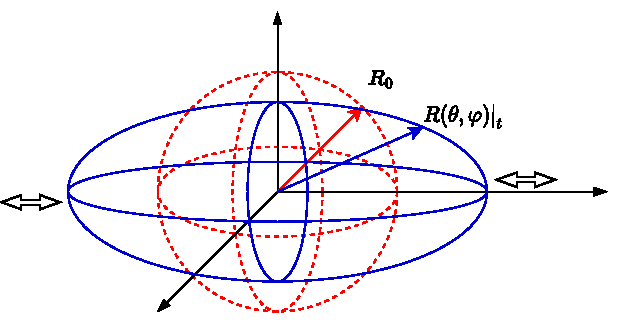
\includegraphics[scale=1.1]{Chapters/Figures/shape_oscillations.pdf}
    \caption{The vibration of a nucleus whose equilibrium shape is a spheroid, with nuclear radius $R_0$ (\emph{average nuclear radius}) and the nuclear radius at a different moment in time.}
    \label{fig-nuclear-vibration}
\end{figure}

By using Eq. \ref{nuclear-shape} which characterizes the \emph{vibrations} of a nuclear surface (via the collective coordinates $\alpha_{\lambda\mu}$), one can give the expression of an initial Hamiltonian of \emph{collective} nature as:
\begin{align}
    H_\text{coll}\equiv T+V=\frac{1}{2}\sum_{\lambda\mu}\left[B_\lambda\left|\frac{\text{d}\alpha_{\lambda\mu}}{\text{d}t}\right|^2+C_\lambda|\alpha_{\lambda\mu}|^2\right]\ ,
    \label{collective-hamiltonian-stiffness-inertia}
\end{align}
Hamiltonian which is in fact both invariant under rotation and time reversal \cite{messiah2014quantum}.  The real numbers $B_\lambda$ and $C_\lambda$ represent \emph{inertial} and \emph{stiffness} parameters for the nuclear matter. The spectrum of such a Hamiltonian after a canonical quantization (see calculations in Ref. \cite{ring2004nuclear} or \cite{bertulani2007nuclear}) will have a harmonic-like structure, depending on the value of $\lambda$. Indeed, by looking at the expression from Eq. \ref{collective-hamiltonian-stiffness-inertia} one can see that it can be brought to a form:
\begin{align}
    H_\text{coll}^\text{osc}=\frac{p^2}{2m}+\frac{1}{2}kr^2\ ,
    \label{eq-bohr-hamiltonian-oscillator-simple}
\end{align}
which is typical to a harmonic oscillator Hamiltonian. The frequency of oscillation of such a Hamiltonian is given by the relation $\omega=\sqrt{k/m}$. The vibrations can now be understood in terms of a sum of harmonic oscillator frequencies, where each frequency is given by $\lambda$:
\begin{align}
\omega_\lambda=\sqrt{\frac{C_\lambda}{B_\lambda}}\ .
\end{align}

The inertia term $B_\lambda$ (also called the \emph{mass parameter}) has the following expression \cite{ring2004nuclear}:
\begin{align}
    B_\lambda=\frac{\rho mR_0^5}{\lambda}=\frac{3}{4\pi\lambda}AmR_0^2\ ,
\end{align}
showing a quadratic dependence with the average nuclear radius. With these ingredients, one can sketch a form of $H_\text{coll}$ similar to Eq. \ref{eq-bohr-hamiltonian-oscillator-simple} in the following manner:
\begin{align}
    H_\text{coll}=\sum_{\lambda\mu}\hbar\omega_\lambda\left(N_{\lambda\mu}+\frac{1}{2}\right)\ ,
\end{align}
where indeed, the typical harmonic oscillator spectrum should be expected for the final collective spectra of nuclei.

The recipe for further manipulation of the Bohr's collective Hamiltonian from Eq. \ref{collective-hamiltonian-stiffness-inertia} is quite a lengthy process \cite{bohr1998nuclear,ring2004nuclear}, with several considerations that are beyond the scope of the current work. Shortly, for the quadrupole deformed nuclei, the expression of the potential term $V$ will be a function that depends on the parameters $(\beta,\gamma)$, potential that is defined as a quadratic approximation in the vicinity of a deformed minimum point $p_0|_\text{min}=(\beta_,\gamma_0)$. This starts from the general assumption that the nucleus has the deformation $p_0$ in the ground state, and the excitations are rotations and small oscillations around this \emph{equilibrium} deformation point. Thus $V(\beta,\gamma)$ can be written as:
\begin{align}
    V(\beta,\gamma)=\frac{1}{2}C_{20}\left(\alpha_{20}(\beta,\gamma)-\alpha_{20}^2\right)^2+\frac{1}{2}C_{22}\left(\alpha_{22}(\beta,\gamma)-\alpha_{22}^0\right)\ .
\end{align}

Choosing the body-fixed axis as a reference system makes the calculations much easier, since the system's axes coincide with the principal axes of the ellipsoid itself. Assuming such a coordinate system and an ellipsoid which possesses axial symmetry, one can write the kinetic term $T$ of the Hamiltonian as a sum of a \emph{rotational} and a \emph{vibrational} part.
\begin{align}
    T=T_\text{vib}+T_\text{rot}\ .
\end{align}

The equations for the two sub-terms are thoroughly demonstrated in Ref. \cite{li2022model}. Their expressions are given in terms of the deformation parameters $(\beta,\gamma)$, the mass parameters $B_2$ (for the quadrupole deformations) and the stiffness parameters $C_2$. Thus, the vibrational term is:
\begin{align}
    T_\text{vib}=\frac{1}{2}B_2\left(\dot{\beta}^2+\beta^2\dot{\gamma}^2\right)\ ,
    \label{kinetic-vibrational-energy-collective}
\end{align}
and the rotational term is:
\begin{align}
    T_\text{rot}=\frac{1}{2}\sum_i\mathcal{I}_i\omega_i^2\ ,
    \label{kinetic-rotational-energy-collective}
\end{align}
where the index $i=1,2,3$ suggests each of the three principal axes of the ellipsoid (this notation is different from the previous notations $x,y,z$ and it will always suggest the body-fixed system). In the expression of $T_\text{rot}$, two crucial physical quantities arise, namely the angular velocities around each body-fixed axis and the functions $\mathcal{I}_k$ that will eventually play the role of \emph{moments of inertia}. However, it is important to analyze the functions $\mathcal{I}_k(\beta,\gamma$) in order to better understand what kind of nature the nucleus exhibit in its rotational and vibrational motion. Ref. \cite{ring2004nuclear} shows that:
\begin{align}
    \mathcal{I}_k=4B_2\beta^2\sin^2\left(\gamma-\frac{2\pi}{3}k\right)\ .
\end{align}

In the case of fixed deformation (that is $\beta$ and $\gamma$ do not change), then the rotational kinetic term represents the energy of a rotor with the moments of inertia $\mathcal{I}_{1,2,3}$, i.e., a \emph{pure rotor}. When the deformation parameters are changing, the rotational and vibrational degrees of freedom will become coupled by the deformation dependence of $\mathcal{I}_k$, leading to a situation that is not specific to a pure rotor. In fact, the functions $\mathcal{I}_k$ will not represent the moments of inertia (MOI) for a rigid rotor anymore. However, a comparison between $\mathcal{I}$, the rigid-like $\mathcal{I}_k^\text{rig}$ MOI, and irrotational-like MOI $\mathcal{I}_k^\text{irr}$ is done experimentally, from determinations of the energy spacing between the first excited states. The last two quantities have the following expressions \cite{bohr1954rotational,ring2004nuclear}:
\begin{align}
    \mathcal{I}_k^\text{rig}&=\frac{2}{5}mAR_0^2\left(1-\sqrt{\frac{5}{4\pi}\beta\cos\left(\gamma-\frac{2\pi}{3}k\right)}\right)\ ,\\
    \mathcal{I}_k^\text{irr}&=\frac{3}{2\pi}mAR_0^2\beta^2\sin^2\left(\gamma-\frac{2\pi}{3}k\right)\ .
    \label{eq-irrotational-rigid-mois}
\end{align}

The dependence of the two types of MOI on the triaxiality parameter $\gamma$ (and fixed $\beta$) can be seen in Fig. \ref{fig-irrotational-rigid-mois}. The differences between the irrotational-like and rigid MOI are as follow:
\begin{itemize}
    \item The irrotational MOI vanish when the ellipsoid has axial symmetry
    \item $\mathcal{I}^\text{irr}$ is much more sensitive to the deformation $\beta$, while the rigid MOI have most of the contribution coming from a typical rigid sphere-like MOI
    \item Determinations of the \emph{experimental} MOI for well-deformed nuclei show that the irrotational MOI is smaller by a factor of almost 3 than the experimental values. Moreover, the rigid MOI show a factor of 2 larger than the experimental values:
    \begin{align}
        \mathcal{I}^\text{irr}<\mathcal{I}^\text{exp}<\mathcal{I}^\text{rig}\ ,
    \end{align}
    suggesting that the \emph{real} flow structure within a nucleus is neither irrotational, nor like a rigid rotator.
\end{itemize}

\begin{figure}
    \centering
    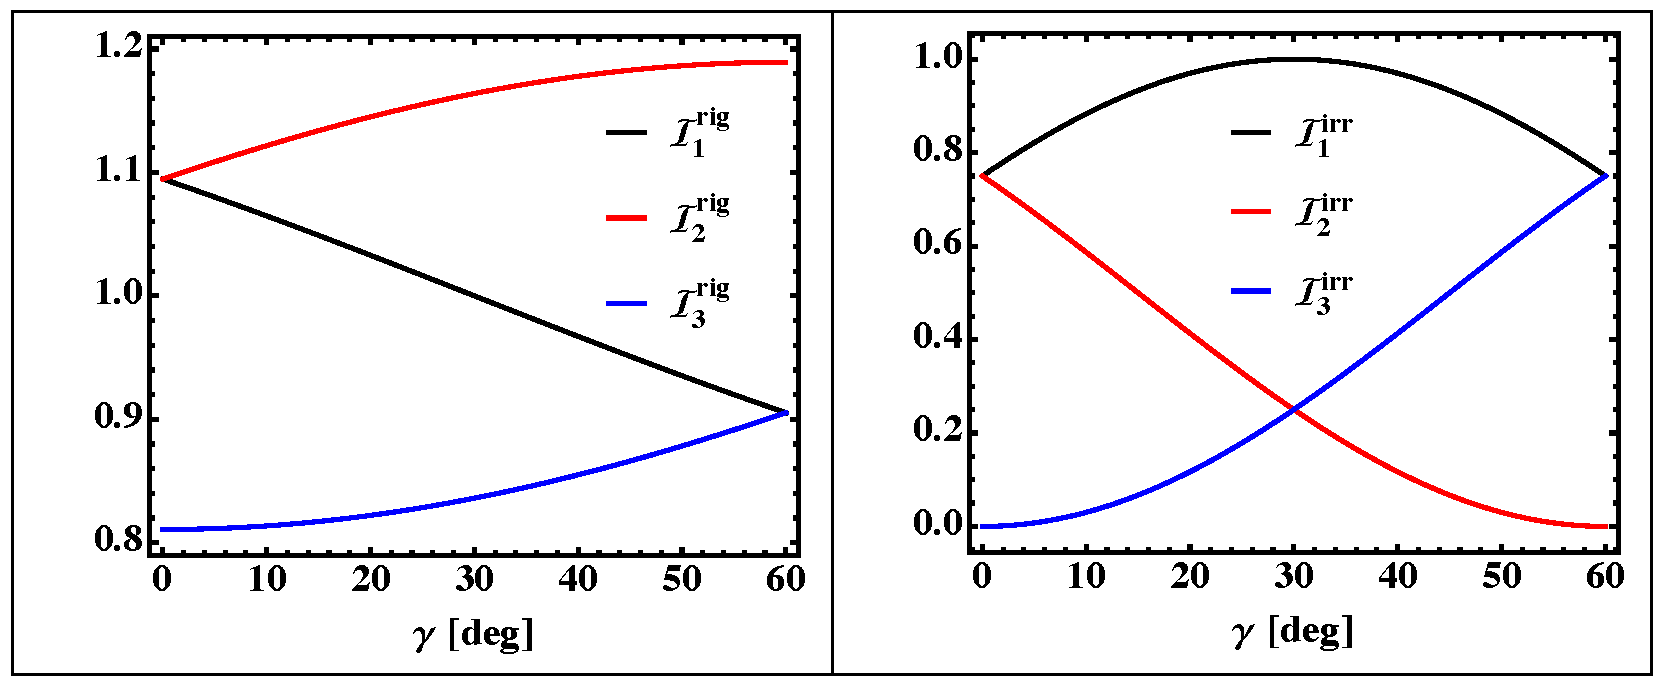
\includegraphics[scale=0.51]{Chapters/Figures/mois_rig_irr.pdf}
    \caption{Comparison between the irrotational-like and the rigid-like MOI defined in Eq. \ref{eq-irrotational-rigid-mois} that are typical for a rigid rotator or the irrotational motion of a fluid. The deformation parameter $\beta$ is $0.3$. Note the vanishing of the irrotational MOI when axial symmetry is present.}
    \label{fig-irrotational-rigid-mois}
\end{figure}

\subsection{Nuclear Vibration}

The energy scheme is composed of levels that are built from these oscillator frequencies. The absorption or emission of vibration-like energy quanta (i.e., phonons) that a nucleus can do (passing to a higher or a lower level) will be in terms of dipole, quadrupole, octupole, etc. vibrating phonons. These excitations will contribute to building the entire spectrum of the nuclei, starting with the ground state: resulting in the so-called \emph{vibrational bands}.
Since the the quadrupole effects are of interest within the current work, the vibrational spectrum specific to quadrupole $\lambda=2$ phonons can be seen in Fig. \ref{fig-vibrational-bands}.
\begin{figure}
    \centering
    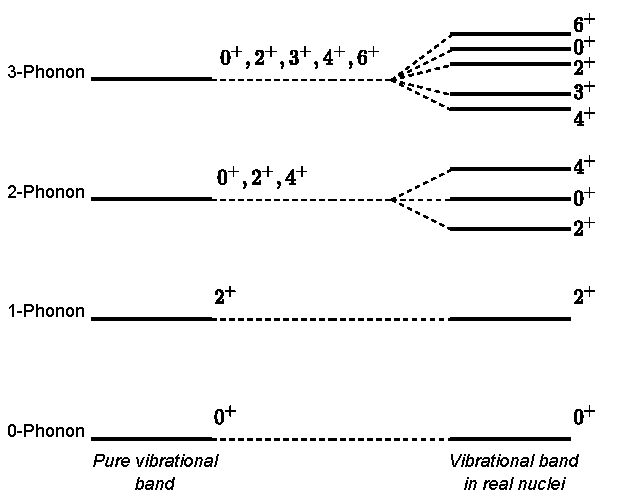
\includegraphics[scale=1.1]{Chapters/Figures/vibrational_states.pdf}
    \caption{An illustrative example with vibrational bands that are built as excitations of multiple phonons on a ground state. The left side contains an ideal harmonic vibrator, with the degenerate spin states indicated for each level. Right side contains the non-degenerate vibrational levels that exist in nuclei. Keep in mind that the each phonon level is built as multiple excitations of a \emph{quadrupole phonon}.}
    \label{fig-vibrational-bands}
\end{figure}

A general rule that is used to construct such vibrational bands is related to the concept of \emph{symmetrized states}. Since the excited quanta are represented by phonons (identical bosons) which have integer angular momentum (e.g., $\lambda=2$ for the quadrupole vibrations) the only spin states than can be observed in such spectra are the ones for which the final angular momenta couple to give symmetric combinations. This is the reason why in the energy state created by exciting the ground state $0^+$ with two phonons, only the states $0^+,2^+,4^+$ appear; the spin states $1^+$ and $3^+$ do not give symmetric combinations. A more generic method for determining which sequence of spins can be obtained by coupling angular momenta of vibrational phonons can be seen in Ref. \cite{ring2004nuclear}.

A quantity which is often used within the measurements of nuclear properties is the ratio between the second and the first excited states within a band. These ratios are usually denoted by $E(4^+)/E(2^+)$ (the state $4^+$ belongs to the triplet phonon state depicted in Fig. \ref{fig-vibrational-bands}), and the theoretical value for the vibrational model gives a value of $2$. However, some experimental results point out to a value close to $2.2$ for nuclei below $A=150$, and a constant value of $3.3$ for $150<A<190$ (refer to Fig. \ref{4state-2state-ratio}). It should be noted that for the latter case, the value of the ratio is specific to another kind of nucleonic motion: \emph{rotation}, which will be discussed in the following section.
Example of experimental \emph{vibrational bands} for several even-$A$ nuclei are shown in Fig. \ref{energy-levels-120Te-virbational-band}.

\begin{figure}
    \centering
    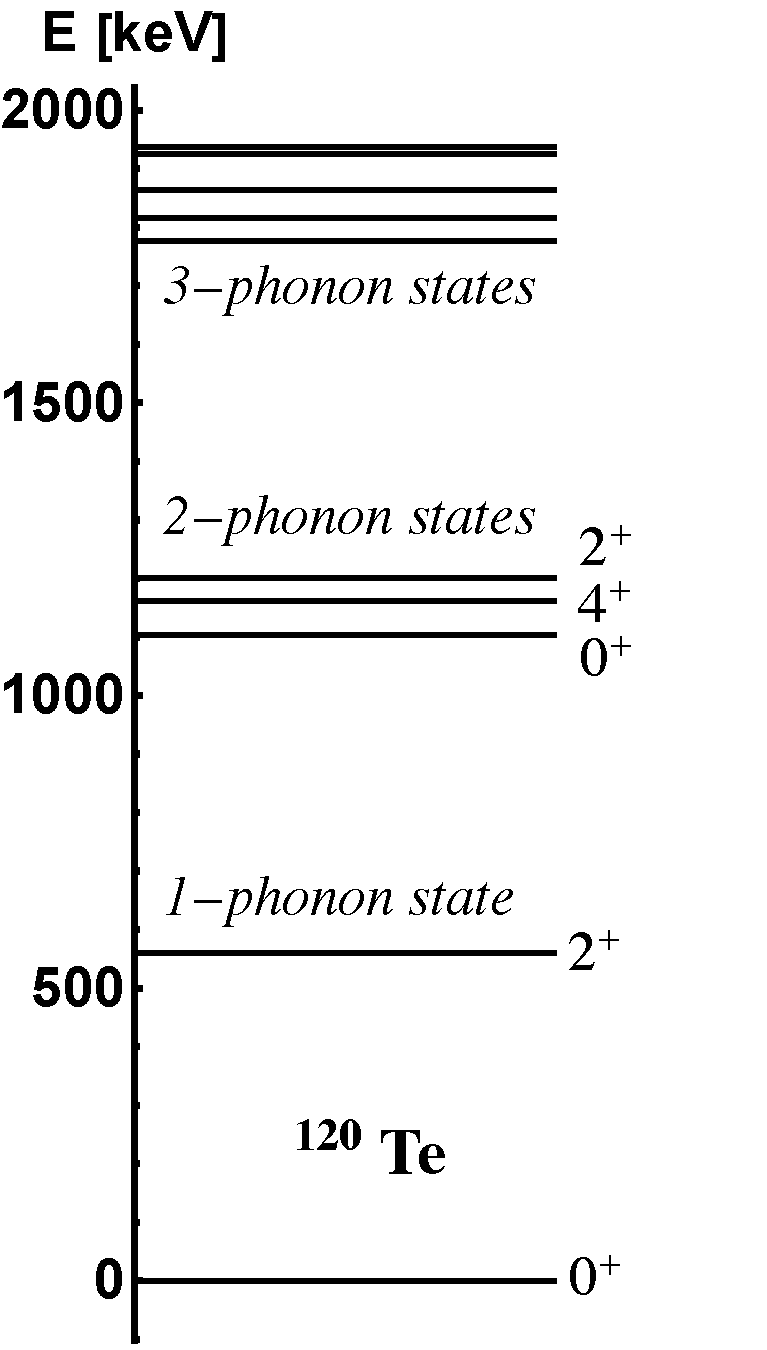
\includegraphics[scale=0.37]{Chapters/Figures/120Te_vib_experimental.pdf}
    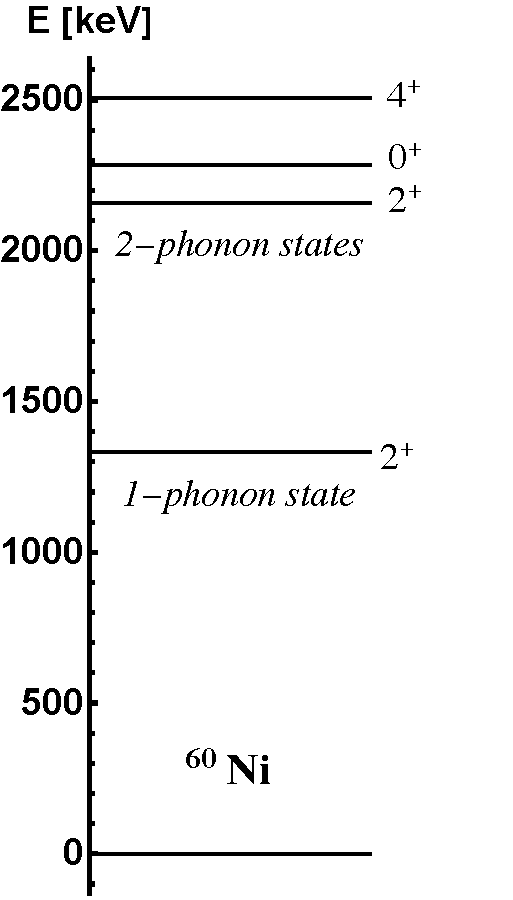
\includegraphics[scale=0.55]{Chapters/Figures/60Ni_vib_experimental.pdf}
    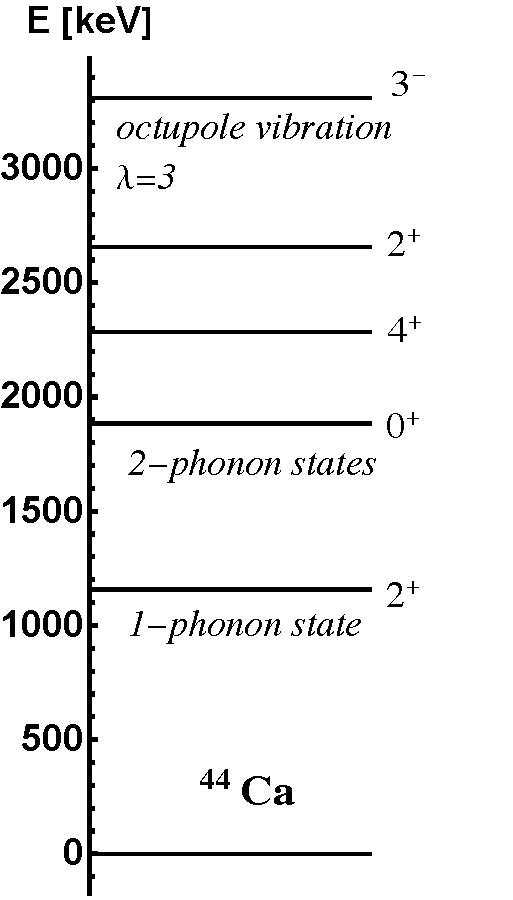
\includegraphics[scale=0.55]{Chapters/Figures/44Ca_vib_experimental.pdf}
    \caption{Vibrational bands in even-$A$ nuclei. \textbf{Left:} The experimental energy levels for $^{120}$Te, showing a vibrational structure for this nucleus. The triplet states that correspond to two excited quadrupole phonons can be seen, together with the quintuplet formed by adding three phonons to the $0^+$ ground state. Experimental data is taken from \cite{kitao2002nuclear}. \textbf{Middle:} The experimental data for $^{60}$Ni. For simplicity, only the first two phonon states are represented. Experimental data for this nucleus was taken from Ref. \cite{browne2013nuclear}. \textbf{Right}: The experimental data for a vibrational-like structure in $^{44}$Ca. Data is taken from Ref \cite{chen2011nuclear}. For the last spectrum, one can observe an energy level coming from the vibrational motion corresponding to an \emph{octupole} mode ($\lambda=3$).}
    % \label{energy-levels-60Ni-virbational-band}    
    \label{energy-levels-120Te-virbational-band}    
\end{figure}

There can also be vibrational bands in odd-$A$ nuclei. Indeed, if one considers the nucleus as a spherical even-even core plus an extra nucleon, the \emph{final} nuclear states are formed by coupling an individual $j$ orbit with the vibrational states of the core.
In the case of odd-$A$ nuclei, one can take the case of $^{63}$Cu, which has the ground state $3/2^{-}$. The g.s. for this nucleus is given by the last \emph{uncoupled} nucleon that occupies a shell. In fact, for this particular nucleus, it is the $2p_{3/2}$ proton that will give the final spin and parity of the nucleus. The vibrational spectrum which arises here can be explained by coupling the aforementioned proton with the even-$A$ core of $^{62}$Ni. Indeed, by taking a $2^+$ vibrational phonon from the even nucleus, then the (odd-proton)+(phonon) system can generate a sequence of energy states that are given by the angular momenta coupling rules (i.e., negative parity states with $I=1/2,3/2,5/2,7/2$ will be formed).
This kind of particle-core coupling that generates sequences of bands will be relevant later on, when discussing the formalism of this work.
The energy levels depicted in Fig. \ref{energy-levels-63Cu-virbational-band} show the particle-core coupling effects on the vibrational structure in odd-mass nuclei.

\begin{figure}
    \centering
    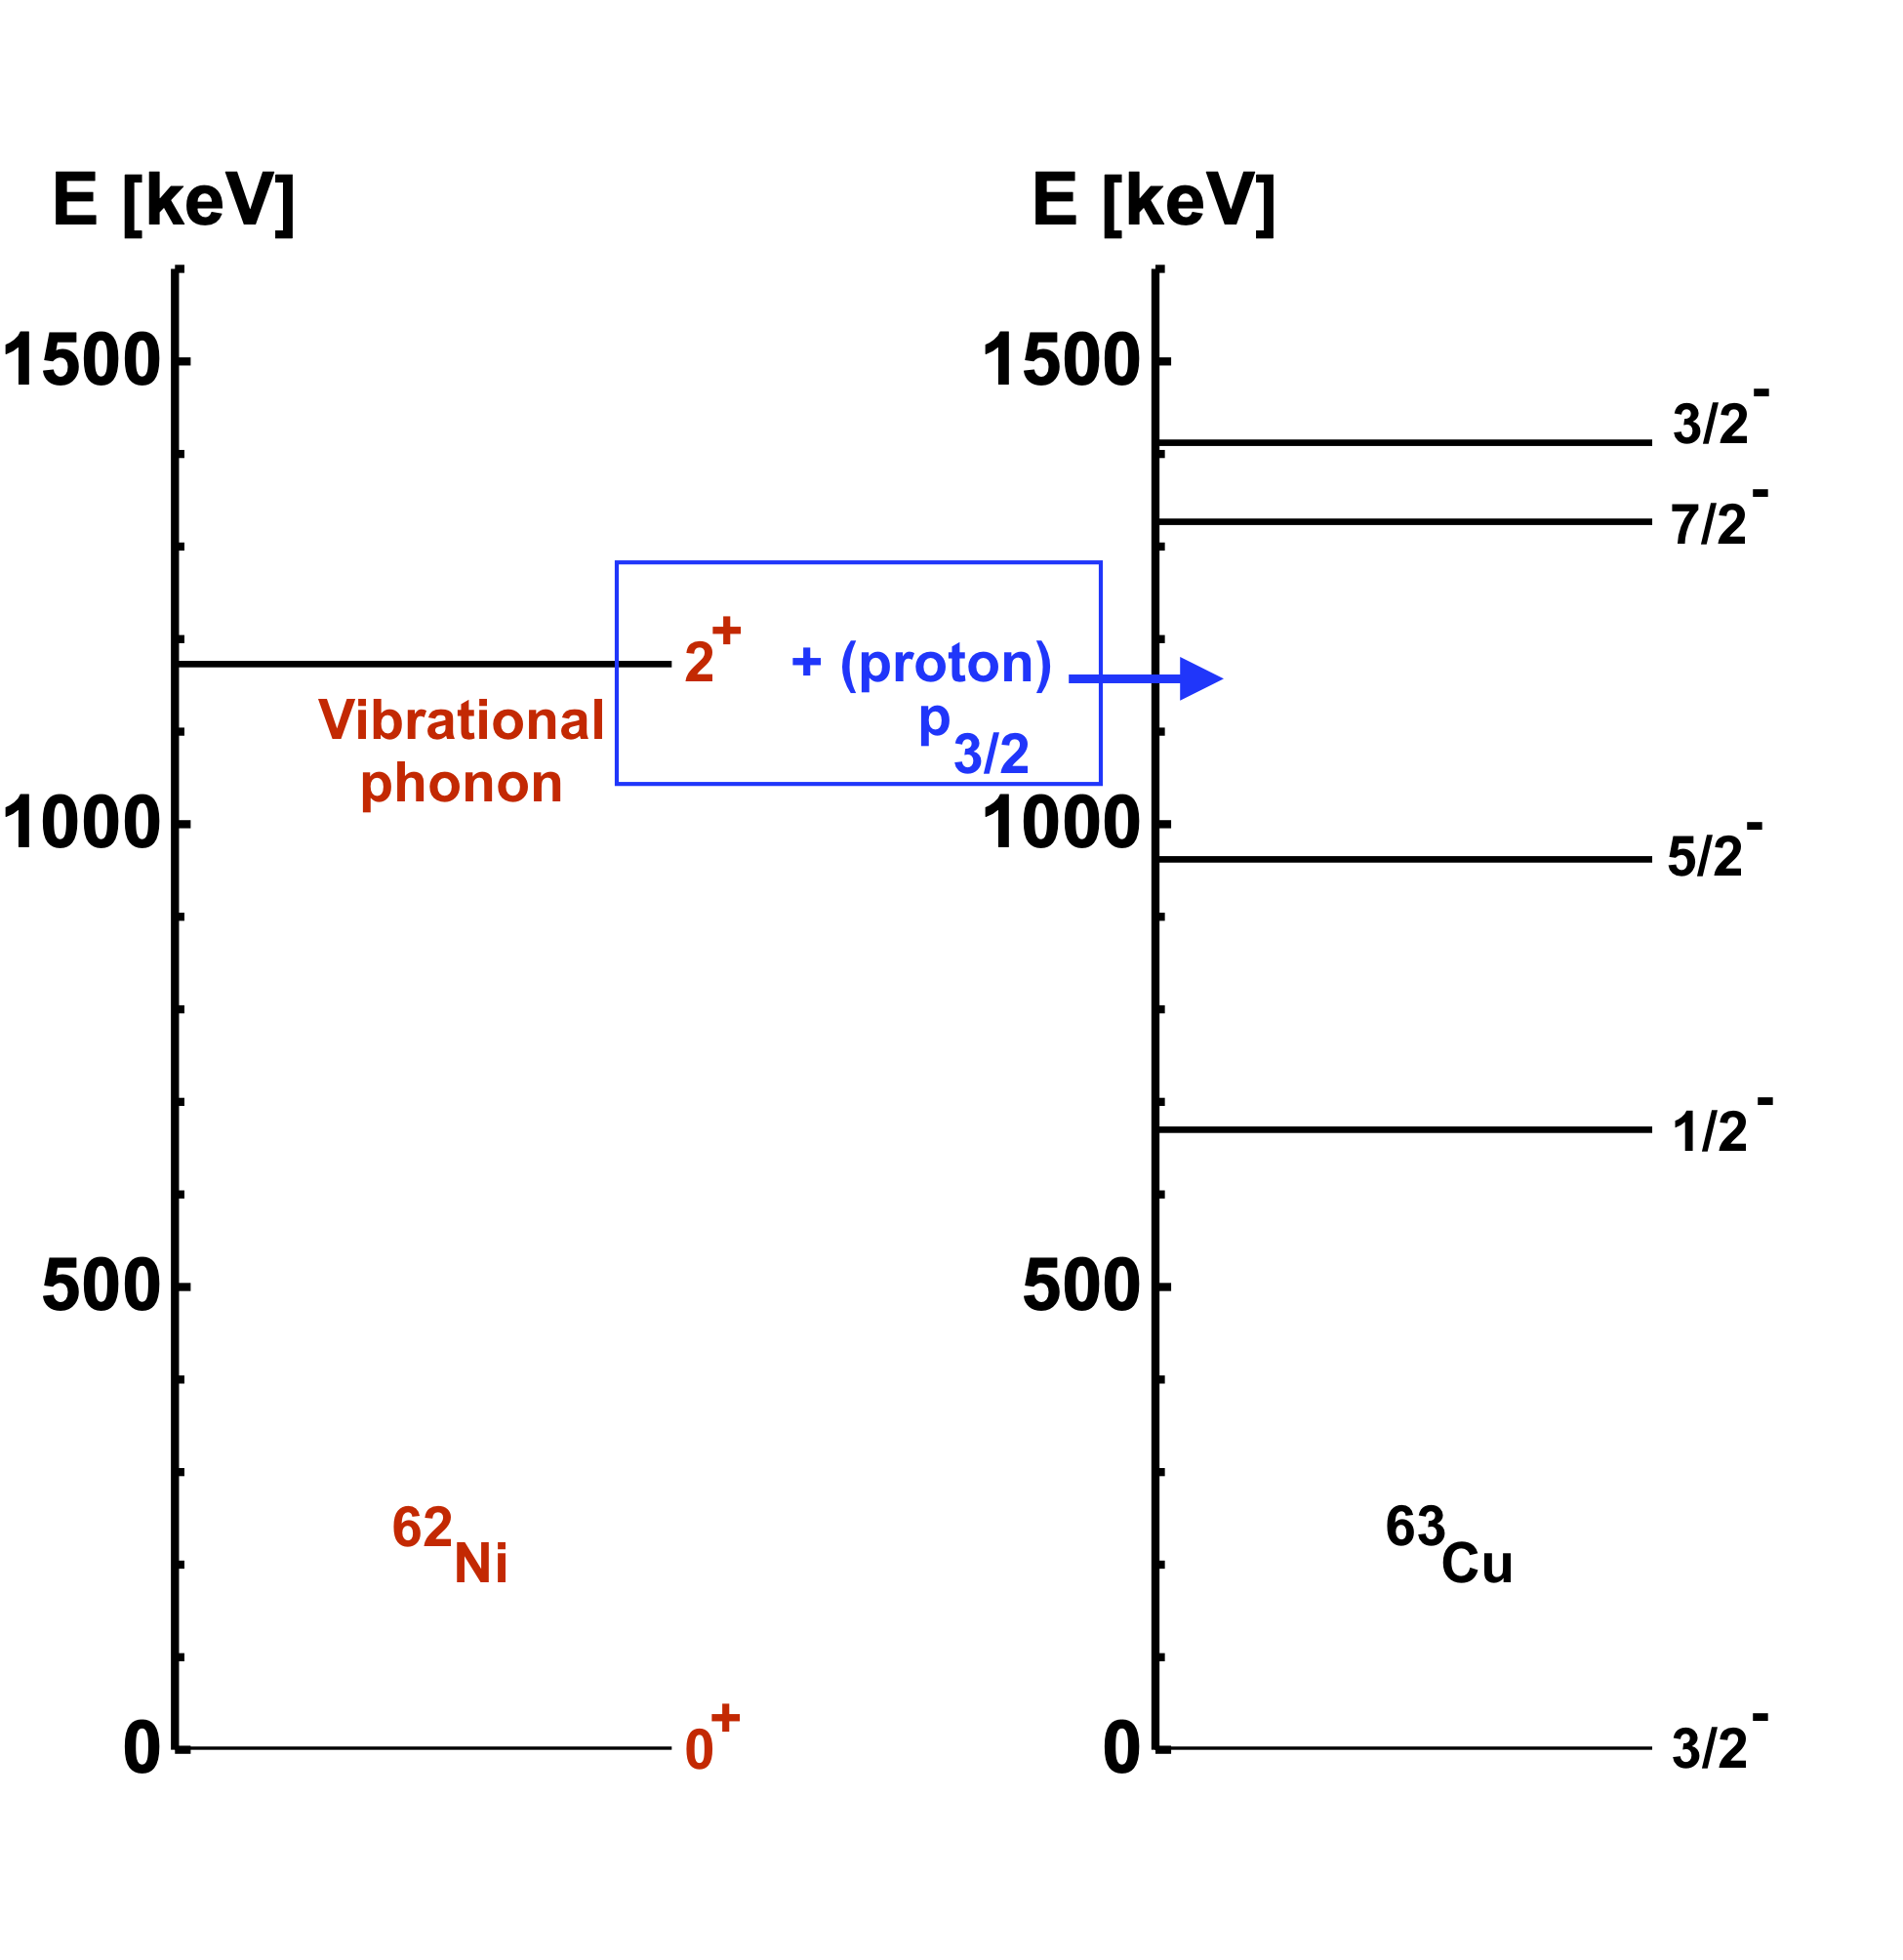
\includegraphics[scale=0.155]{Chapters/Figures/63Cu_vib_experimental.png}
    \caption{The experimental data of the vibrational states in $^{63}$Cu. The $2^+$ phonon state in $^{62}$Ni is also shown for a clearer picture. The experimental data for $^{62}$Ni was taken from Ref. \cite{nichols2012nuclear} and for $^{63}$Cu was taken from Ref. \cite{erjun2001nuclear}. The blue rectangle tries to emphasize that the states quadruplet is formed by the coupling of odd proton to the $2^+$ vibrational state from the neighboring nucleus.}
    \label{energy-levels-63Cu-virbational-band}
\end{figure}

\subsection{Nuclear Rotation}

The quantization procedure for the collective Hamiltonian is a tedious procedure which can be followed in the work of Corrigan et al. \cite{corrigan1976exact}. However, the only interest is for the rotational-kinetic term from $H_\text{coll}$. This term is called the \emph{rotational energy}, and its expression is given by:
\begin{align}
    \hat{T}_\text{rot}=\frac{\hat{I}_1^2}{2\mathcal{I}_1}+\frac{\hat{I}_2^2}{2\mathcal{I}_2}+\frac{\hat{I}_3^2}{2\mathcal{I}_3}\ .
    \label{eq-rotational-energy-quantized}
\end{align}

The three operators that appear in Eq. \ref{eq-rotational-energy-quantized} are in fact the projections of the total angular momentum $\mathbf{I}$ on the body-fixed axes (see Fig. \ref{rotational-coupling-schematic} for reference). Note that throughout the text, the angular momentum will be interchangeably represented with an arrow or just by bold letters.

An important conclusion which comes out from the work of Bohr and Mottelson \cite{bohr1954rotational} (also see discussion in Ref. \cite{greiner1996nuclear}) is that no rotations are possible for spherical nuclei nor for axially deformed nuclei which are rotating about the symmetry axis. Consequently, a prior deformation (e.g., of quadrupole type) and a rotating axis which does not coincide with the symmetry one are required for the appearance of rotational levels. Indeed, every nucleus which contains energy states that are generated by the rotational motion has these bands due to the rotation about an axis that is different from the symmetry axis, and its shape is either axially-symmetric or axially-asymmetric \cite{hamamoto2016interplay}.

A nucleus can generate angular momentum in two ways:
\begin{enumerate}
    \item collectively, via combined rotations and vibrations of the nuclear droplet (the rotation+vibration spectrum of a nucleus will be shown in the next section)
    \item single-particle excitations: unpaired nucleons can rearrange themselves in such a way that they account to the nuclear spin 
\end{enumerate}

The coupling of the rotational angular momentum $\mathbf{R}$ of the droplet with the single-particle angular momentum of a valence nucleon $\mathbf{j}$ can be seen in Fig. \ref{rotational-coupling-schematic}.
\begin{figure}
    \centering
    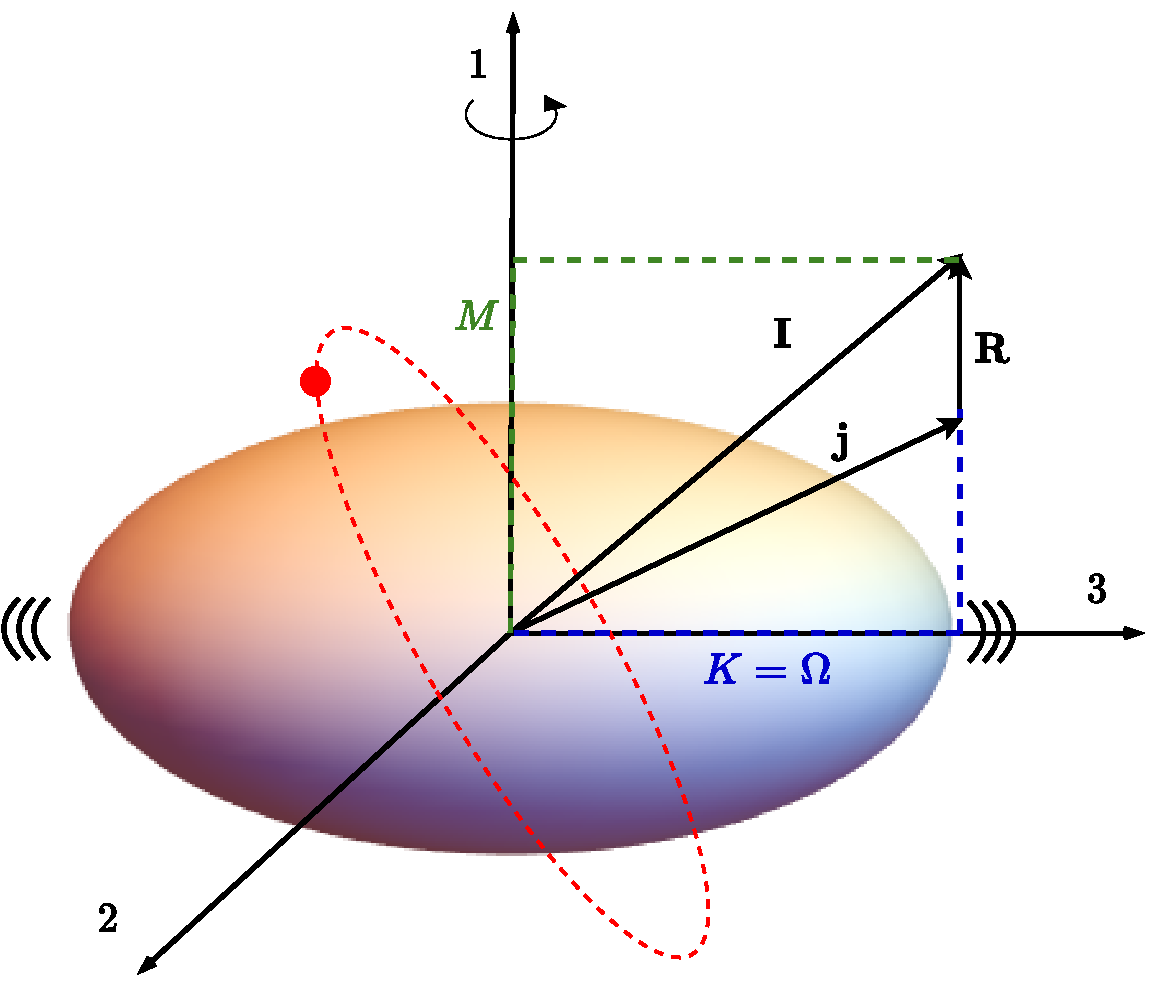
\includegraphics[scale=0.5]{Chapters/Figures/SCHEMATIC_COUPLING_ROTATIONAL.pdf}
    \caption{The coupling of the collective angular momentum with the angular momentum of a single-particle, for an axially deformed nucleus that is rotating about an axis perpendicular to the deformation axis.}
    \label{rotational-coupling-schematic}
\end{figure}

Based on the expression of $T_\text{rot}$ from Eq. \ref{kinetic-rotational-energy-collective}, its quantized form given in Eq. \ref{eq-rotational-energy-quantized}, and the coupling scheme depicted in Fig. \ref{rotational-coupling-schematic}, it is possible to construct a Hamiltonian that corresponds to rotating nucleus which has no valence particle. More precisely, the $\mathbf{j}$ term is neglected, such that only the pure collective motion of a nucleus is emphasized ($\mathbf{I}=\mathbf{R}$). This approximation is however only valid for even-even nuclei and for the low-lying states \cite{bertulani2007nuclear,davydov1958rotational}:
\begin{align}
    H&=H_\text{rot}+H_\text{intr}=\sum_i\frac{\hbar^2}{2\mathcal{I}_i}R_i^2\ ,
\end{align}
where the second term $H_\text{intr}$ represents some effects coming from the internal structure of the rotator itself. However, most of the time these terms can be neglected, leading to a rather simple energy spectrum for the even-even nuclei:
\begin{align}
    E_\text{rot}(I)=\frac{\hbar^2}{2\mathcal{I}_\perp}I(I+1)\ .
    \label{eq-simple-rotor-spectrum}
\end{align}

In the above expression, the MOI $\mathcal{I}_\perp$ corresponds to an axis that is perpendicular to the symmetry axis (i.e., either $1$-axis or the $1$-axis) of the ellipsoid. In the case of axial symmetry both moments are equivalent, such that the general notation $\mathcal{I}_\perp$ is made. As an observation, since there is no single-particle contribution, the quantized angular momentum $I$ (or spin) is equivalent to $R$. The spectrum defined by Eq. \ref{eq-simple-rotor-spectrum} leads to energy spacings $\propto I(I+1)$, which is also met in the  molecular spectra. The ground-state will always be the state $0^+$, and due to the mirror symmetry that is required for the wave-functions describing the even-even nuclei \cite{ring2004nuclear}, every other excited state will be represented by an even value of the spin: $2^+,4^+,\dots$.
The ratio $E(4^+)/E(2^+)$ for these bands is $3.33$ (as it was previously mentioned). This is indeed the best signature for the rotational phenomena in nuclei, indicating a clear presence of deformation + rotational motion. In a previous work by the current team (Raduta et al.) \cite{raduta2017semiclassical}, some spectra of even-even $^{158}$Er were studied and agreement with the observed experimental data was impressive. The energy spectra obtained from Eq. \ref{eq-simple-rotor-spectrum} has a classical counterpart which is known within literature as the \emph{symmetric top}. Fig \ref{rotational-bands-even-even} shows some examples of rotational bands in even mass nuclei, where the $K^pi=0^+$ band head is the ground-state, and every excited state has $\Delta I=2$ units of angular momentum.

\begin{figure}
    \centering
    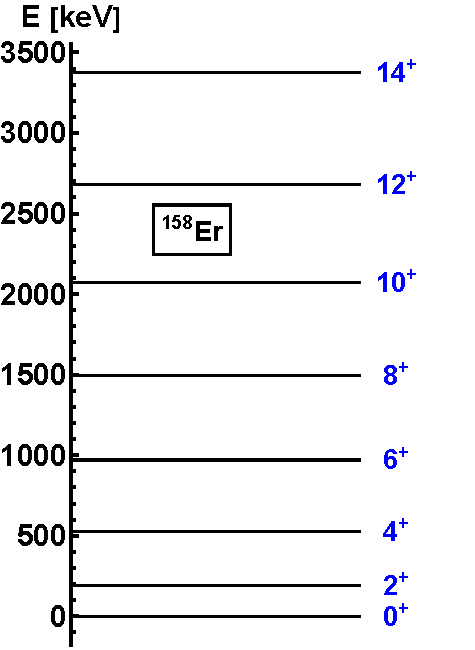
\includegraphics[scale=0.7]{Chapters/Figures/Er158-Rotational-Bands.pdf}
    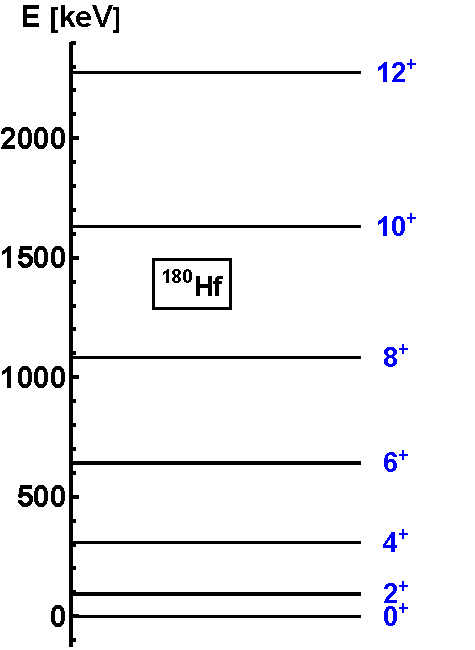
\includegraphics[scale=0.7]{Chapters/Figures/Hf180-Rotational-Bands.pdf}
    \caption{Experimental data showing the rotational bands in even-even nuclei. Note the spacing between the states that increases with $I$ via the rule from Eq. \ref{eq-simple-rotor-spectrum}. Experimental data are taken from Refs. \cite{nica2017nuclear,mccutchan2015nuclear} for each nucleus.}
    \label{rotational-bands-even-even}
\end{figure}

However, the spectra of a simple rigid rotator assumes that the projection $K$ of the total angular momentum for the ground-state of even-even nuclei is $K=0$. So the next step is to consider more general cases of nuclear rotation. There are two general cases of rotational bands that can occur, and both require the coupling scheme of a rotor with a valence nucleon, such that the angular momentum will be $\mathbf{I}=\mathbf{R}+\mathbf{j}$ (so both situations will correspond to odd-$A$ nuclei). The two situations are called \emph{Deformation aligned bands} and \emph{Rotation aligned bands} \cite{uwitonze2015assignment}. Graphical representation with both rotational schemes can be seen in Fig. \ref{ral-dal-coupling-bands}.

\begin{figure}
    \centering
    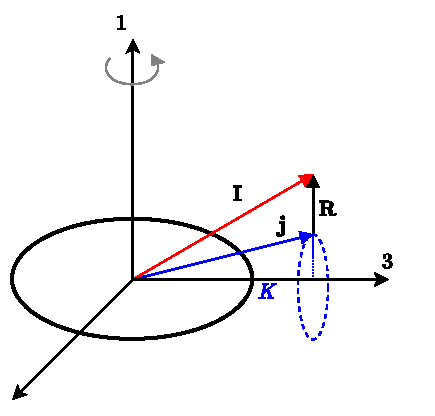
\includegraphics[scale=0.9]{Chapters/Figures/DAL_scheme.pdf}
    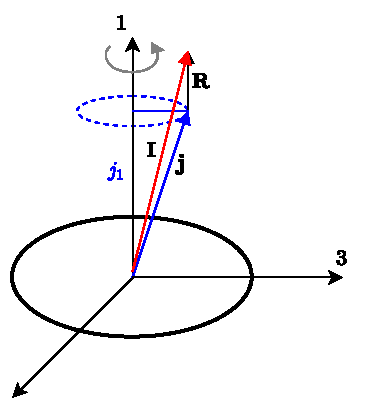
\includegraphics[scale=0.9]{Chapters/Figures/RAL_scheme.pdf}
    \caption{A sketch with the geometrical interpretation of the two ways a nucleus can exhibit rotational bands: Deformed Aligned Bands (\textbf{left}) and Rotation Aligned Bands (\textbf{right}). See text for explanations. The projections of the single-particle's total a.m. on the deformation and rotation axes are denoted with $K$ and $j_1$, respectively.}
    \label{ral-dal-coupling-bands}
\end{figure}

\subsubsection*{Deformation Aligned Bands}

This case is also referred to as \emph{strong-coupling} limit \cite{bohr1953collective} since the particle's a.m. is tightly coupled to the deformation axis (i.e., the symmetry axis). The general Hamiltonian will be:
\begin{align}
    H_\text{rot}=H_0+H_\text{coupl}\ ,
\end{align}
where $H_0$ is the already discussed operator containing the squared components $I_k$ of $\mathbf{I}$ and the extra \emph{coupling term} represents the Coriolis force \cite{bertulani2007nuclear}. The Coriolis effect is reflected by the coupling of the collective motion of the nucleus to the odd nucleon's motion. Despite that, it can be neglected at small rotations.

The projection of the particle's a.m. on the symmetry axis is a good quantum number, and if $\mathbf{R}$ is pointing in a direction that is perpendicular to the deformation axis, then $\Omega=K$, meaning that the energy spectrum will be given by:
\begin{align}
    E_\text{rot}(I)=\frac{\hbar^2}{2\mathcal{I}_\perp}\left[I(I+1)-K(K+1)\right]\ ,
\end{align}
or more formally:
\begin{align}
    E_\text{rot}(I)=\frac{\hbar^2}{2\mathcal{I}_\perp}\left[I(I+1)-K^2\right]+E_0(K)\ .
\end{align}
The rotational band will be constructed on the ground-state $E_0(K)$, where to total spin $I$ will be composed of a sequence $I=K,K+1,K+2,\dots$ and $K\neq\frac{1}{2}$. Consequently, this situation will lead to rotational bands where the difference between two consecutive states is only une unit of angular momentum. It should be pointed out that odd-$A$ nuclei can have multiple rotational bands that are built on different values of $K$.

For $K=\frac{1}{2}$, the band structure will follow:
\begin{align}
    E_\text{rot}(I)=\frac{\hbar^2}{2\mathcal{I}_\perp}\left[I(I+1)+a(-)^{I+\frac{1}{2}}(I+\frac{1}{2})\right]\ .
    \label{deformation-aligned-energy}
\end{align}

The nature of $(-1)^{I+1/2}$ will be explained for \emph{Rotation Aligned Bands}. Moreover, the term $a$ is called the \emph{decoupling parameter} \cite{bertulani2007nuclear}, and it can be determined from the first two experimental energy levels.  Experimental data which point out the presence of rotational bands with $K=1/2$ and $K\neq 1/2$ are shown in Fig. \ref{rotational-bands-odd-a}, for two odd-$A$ nuclei.

\begin{figure}
    \centering
    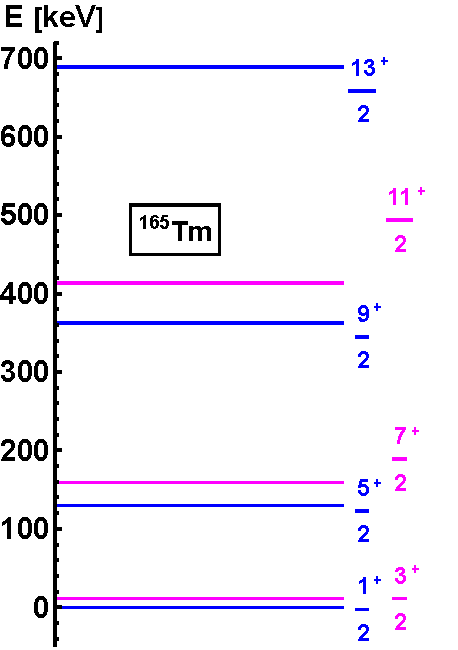
\includegraphics[scale=0.7]{Chapters/Figures/Tm165-Rotational-Bands.pdf}
    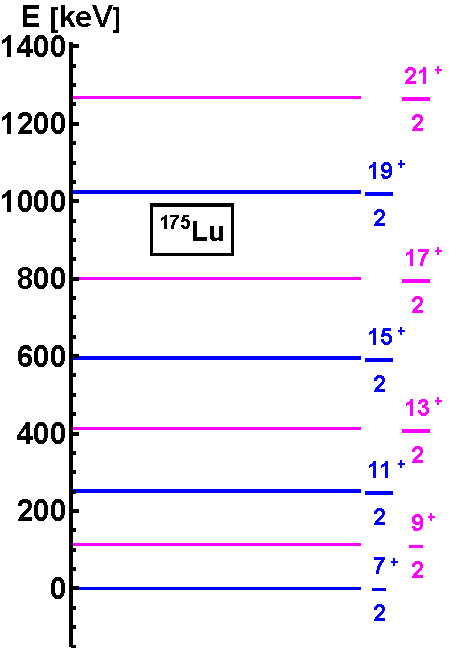
\includegraphics[scale=0.7]{Chapters/Figures/Lu175-Rotational-Bands.pdf}
    \caption{Rotational bands in odd-$A$ nuclei with the $K$ quantum number equal to $K=1/2$ (\textbf{left}) and $K\neq 1/2$ (\textbf{right}).}
    \label{rotational-bands-odd-a}
\end{figure}

\subsubsection*{Rotation Aligned Bands}

This situation is also called the \emph{decoupling limit} \cite{bohr1998nuclear} and it leads to the apparition of \emph{decoupled bands}. Here the total angular momentum is more aligned to the axis of rotation, and its maximum projection is along this axis. This is usually happening at high-spins, meaning strong rotational motion, which makes the angular momentum of the odd-particle to depart from the symmetry axis and align more and more with the direction of rotation (through the Coriolis effect). As such, the coupling term $H_\text{coupl}$ from $H_\text{rot}$ is not neglected here:
\begin{align}
    H_\text{rot}=\frac{\hbar^2}{2\mathcal{I}_\perp}\left(\mathbf{I}^2+\mathbf{j}^2-2\mathbf{I}\cdot\mathbf{j}\right)\ .
\end{align}

It is usually preferred to work with the \emph{raising} and \emph{lowering} operators which correspond to the angular momentum operator: $\mathbf{I}_\pm=\mathbf{I}_1\pm i \mathbf{I}_2$ (equivalently can be done for $\mathbf{j}$), bringing $H_\text{rot}$ to the following expression:
\begin{align}
    H_\text{rot}&=\frac{\hbar^2}{2\mathcal{I}_\perp}\hat{I}^2+\frac{\hbar^2}{2\mathcal{I}_\perp}\hat{j}^2-\frac{\hbar^2}{\mathcal{I}_\perp}K^2+H_\text{Coriolis}\ ,\\
    H_\text{Coriolis}&=-\frac{\hbar^2}{2\mathcal{I}_\perp}(\mathbf{I}_+\mathbf{j}_-+\mathbf{I}_-\mathbf{j}_+)\ .
\end{align}

It is worth pointing out that the effect of the Coriolis term is to couple bands which differ in $K$ quantum number with one unit, effect which is negligible at high deformations and low spins (since the single-particle motion is tightly bound to the bulk nucleus) while at very high rotations (spins) it becomes significant. Consequently, the Coriolis effect most probably occurs in prolate nuclei for an `almost empty' $j$-shells and oblate nuclei for an `almost full' $j$-shell.

When the single-particle angular momentum is orienting itself to the direction of rotation, the projection of $\mathbf{j}$ can be denoted by $j_1$ (keeping a consistency with Fig. \ref{rotational-coupling-schematic}). The spectrum of the decoupled bands will be:
\begin{align}
    E_\text{rot}(I)=\text{const.}+\frac{\hbar^2}{2\mathcal{I}_\perp}(I-j_1)(I-j_1+1)\ ,
\end{align}
where the coupling terms have been embedded in the constant term. This leads to a spin sequence $I=j_1,j_1+2,j_1+4\cdots$, which differs from the previous case via the constant $2\hbar$ angular momentum difference of two consecutive levels.

In order to understand the terms $(-1)^{I+1/2}$ from Eq. \ref{deformation-aligned-energy}, it is required to describe the wave-function corresponding to the particle-core system. Indeed, using the specific quantum numbers $I,K,M$ with their meaning explained in Fig. \ref{rotational-coupling-schematic}, the wave-function will be written as a combination of rotational (the Wigner $D_{MK}^I$ functions) and single-particle components \cite{wang2007exotic,davydov1958rotational}:
\begin{align}
    \Psi_{MK}^I=\ket{IMK}=N\left[\phi_K D_{MK}^I+(-)^{I+K}\phi_{-K}D_{M-K}^I\right]\ ,
\end{align}
where $N$ is the normalization constant, usually having the value $N_I=\sqrt{\frac{2I+1}{16\pi^2}}$. This linear combination of states with $K$ and $-K$ induces a degeneracy and it is due to the invariance of such a system with respect to rotations by $\pi$ around the rotational axis \cite{frauendorf1997tilted,bohr1998nuclear}. The factor $(-)^{I+K}\equiv\alpha$ is called the \emph{signature} and it reflects wether a system is invariant or not to such a rotation. More precisely, the \emph{signature quantum number} is given as \cite{sun1994varied}:
\begin{align}
    \alpha_I=\frac{1}{2}(-)^{I-\frac{1}{2}}\ ,
\end{align}
for a state of spin $I$ in an odd-$A$ nucleus, resulting in the favored states having $\alpha_\textbf{favored}=\frac{1}{2}$ and the unfavored states having $\alpha_\text{unfavored}=-\frac{1}{2}$.

Depending on the signature, the nuclear states can be divided into two sets: one that follows $I=K,K+2,K+4,\dots$ and $I=K+1,K+3,K+5,\dots$. This is the reason why for the decoupled bands, one can regard them as an `initial' rotational band $I,I+1,\dots$ that is `broken' apart in two sequences: one that is favored and one that is unfavored (opposite signature).
An example is a nucleus with odd-$A$, where the favored bands have spins $I_\text{favored}=\frac{1}{2},\frac{5}{2},\frac{1}{2},\dots$, while their unfavored \emph{partner} bands have spins $I_\text{unfavored}=\frac{3}{2},\frac{7}{2},\frac{11}{2},\dots$ and opposite signature (also known as \emph{signature partners}). In fact, taking a closer look at the rotational bands specific to odd-$A$ nuclei shown in Fig. \ref{rotational-bands-odd-a}, each consecutive level is a state with different signature, meaning that each `group' of colors classifies into a set of favored (blue) and unfavored (magenta) states.

This divided set of partner bands also has some characteristics that can be observed throughout experimental measurements. Firstly, the splitting of the two branches implies that the favored states will generally have lower excitation energy than their unfavored partners. This is also proved by the expression of the rotor energy given in Eq. \ref{deformation-aligned-energy}, where the decoupling parameter will cause an upward (downward) shift in energy for states with $I=1/2,5/2,9/2,\dots$ ($I=3/2,7/2,11/2,\dots$), depending whether $a$ is positive (negative). The experimental data shown in Fig. \ref{level-scheme-signature-splitting} shows how the favored partner lies lower with respect to its unfavored partner bands, each having the corresponding spin sequence $\Delta I=2$ for intraband states and $\Delta I=1$ for interband states. Such spectra are very often met in the decay schemes for odd-mass nuclei in which the rotational motion is governed by the (core+particle) coupling scheme.
\begin{figure}
    \centering
    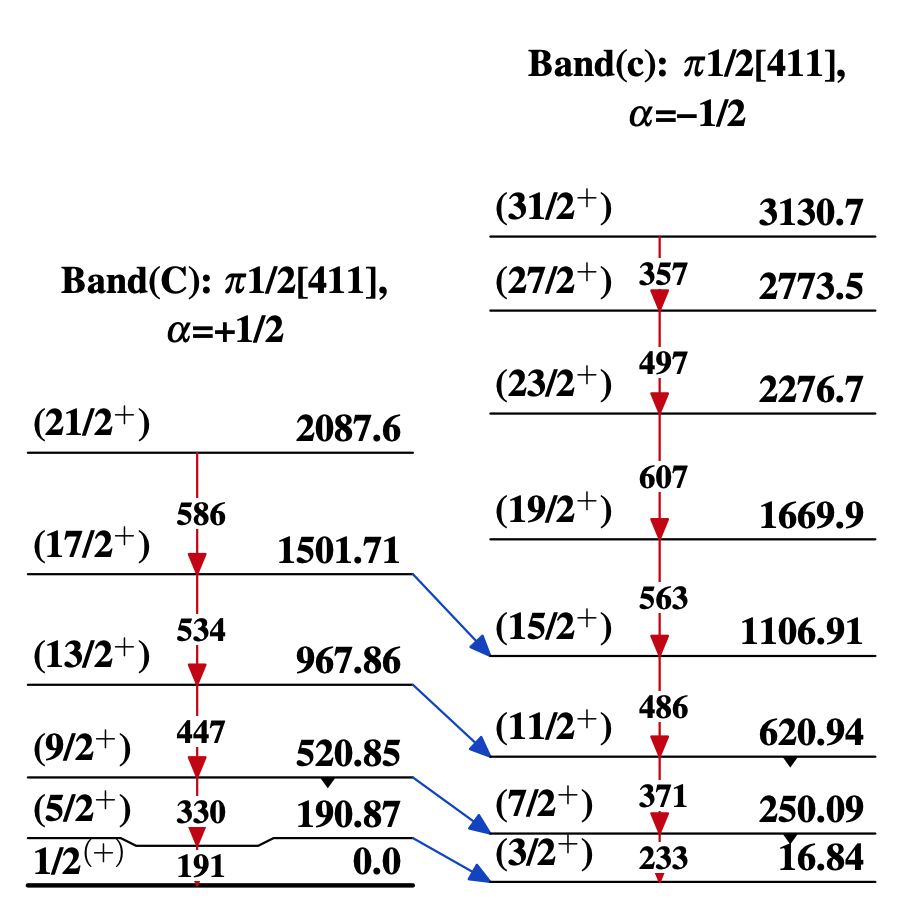
\includegraphics[scale=0.45]{Chapters/Figures/Lu_163_K12-band.png}
    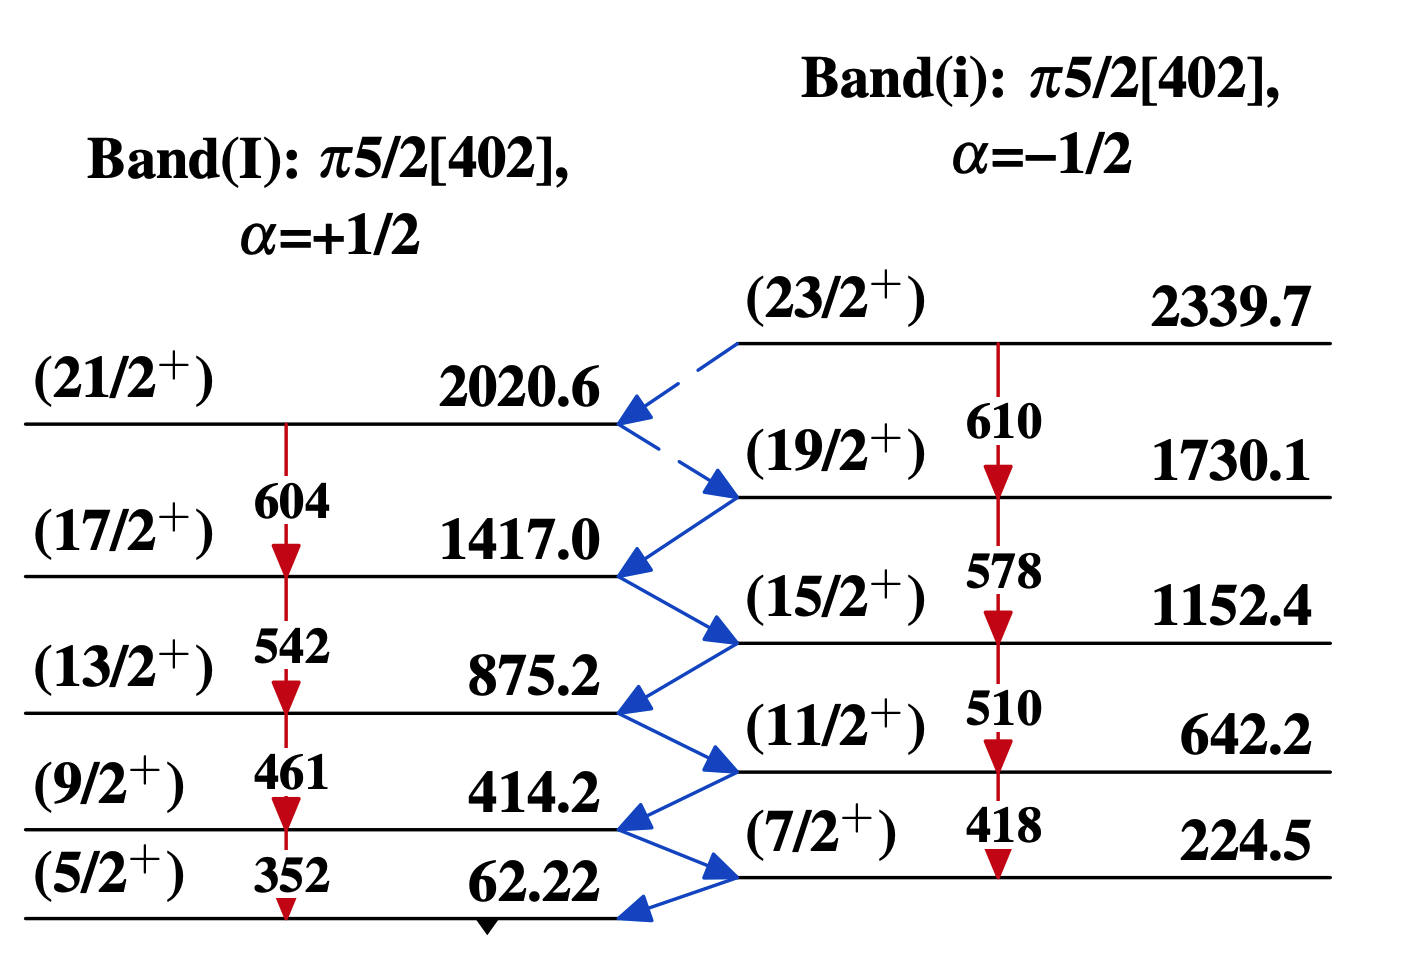
\includegraphics[scale=0.28]{Chapters/Figures/Lu_163_signatureSplitting.png}
    \caption{Experimental level schemes for $^{163}$Lu showing pairs of signature partner bands. \textbf{Left}: the two bands are built on a proton with $j=1/2$ and positive parity. \textbf{Right}: sequences built on a proton with $j=5/2$ with the same parity. The Nilsson quantum numbers are defined for each band. Note the spin difference between each state, as described in text. Also note the lower energies for the favored states. Interband transitions are marked with the blue arrows. These figures were taken from Ref. \cite{reich2010nuclear}.}
    \label{level-scheme-signature-splitting}
\end{figure}

\subsection{Superimposed Rotations and Vibrations}

Up until now, the two types of nuclear motion, namely the collective rotations and vibrations were discussed separately. The small vibrations of the nuclear surface lead to the presence of band structures constructed via the quadrupole phonons carrying $\lambda=2$ units of angular momentum. The collective nature of the nucleus together with effects coming from the coupling a core to a valence nucleon also showed that some rotational band structures can appear in nuclei.

\subsection{Collective Quantities}

In this section, some important quantities will be described since their meaning is strictly related to the collective nature of nuclei. Indeed, one can understand nuclear deformation, energy spectra, and behavior with respect to spin of nuclei by studying quantities such as \emph{rotational frequencies}, \emph{moments of inertia}, \emph{quadrupole moments}, and so on. As it will be shown, the values of such physical observables will point out, for example, if some nuclei experience large deformations, or if rotation causes the nucleus to exhibit excited states. Moreover, the comparison with experimental data for these quantities can help validate some assertions that are initially made, which is usually the crucial test of new models and frameworks that are developed by the nuclear physics community.

\subsubsection*{R - Energy ratio}

As discussed before, the energy ratio between the first excited $4^+$ state to the first excited $2^+$ state is a very good test for checking wether a nucleus `tends' to show rotational or vibrational structures (i.e., spectra). Casten et al. \cite{casten2000nuclear} shows the evolution of this ratio across the mass number $A$, and a classification between \emph{vibrational} vs. \emph{rotational} character can be made. Fig. \ref{4state-2state-ratio} contains the ratio $R_{4^+/2^+}$.

\begin{figure}
    \centering
    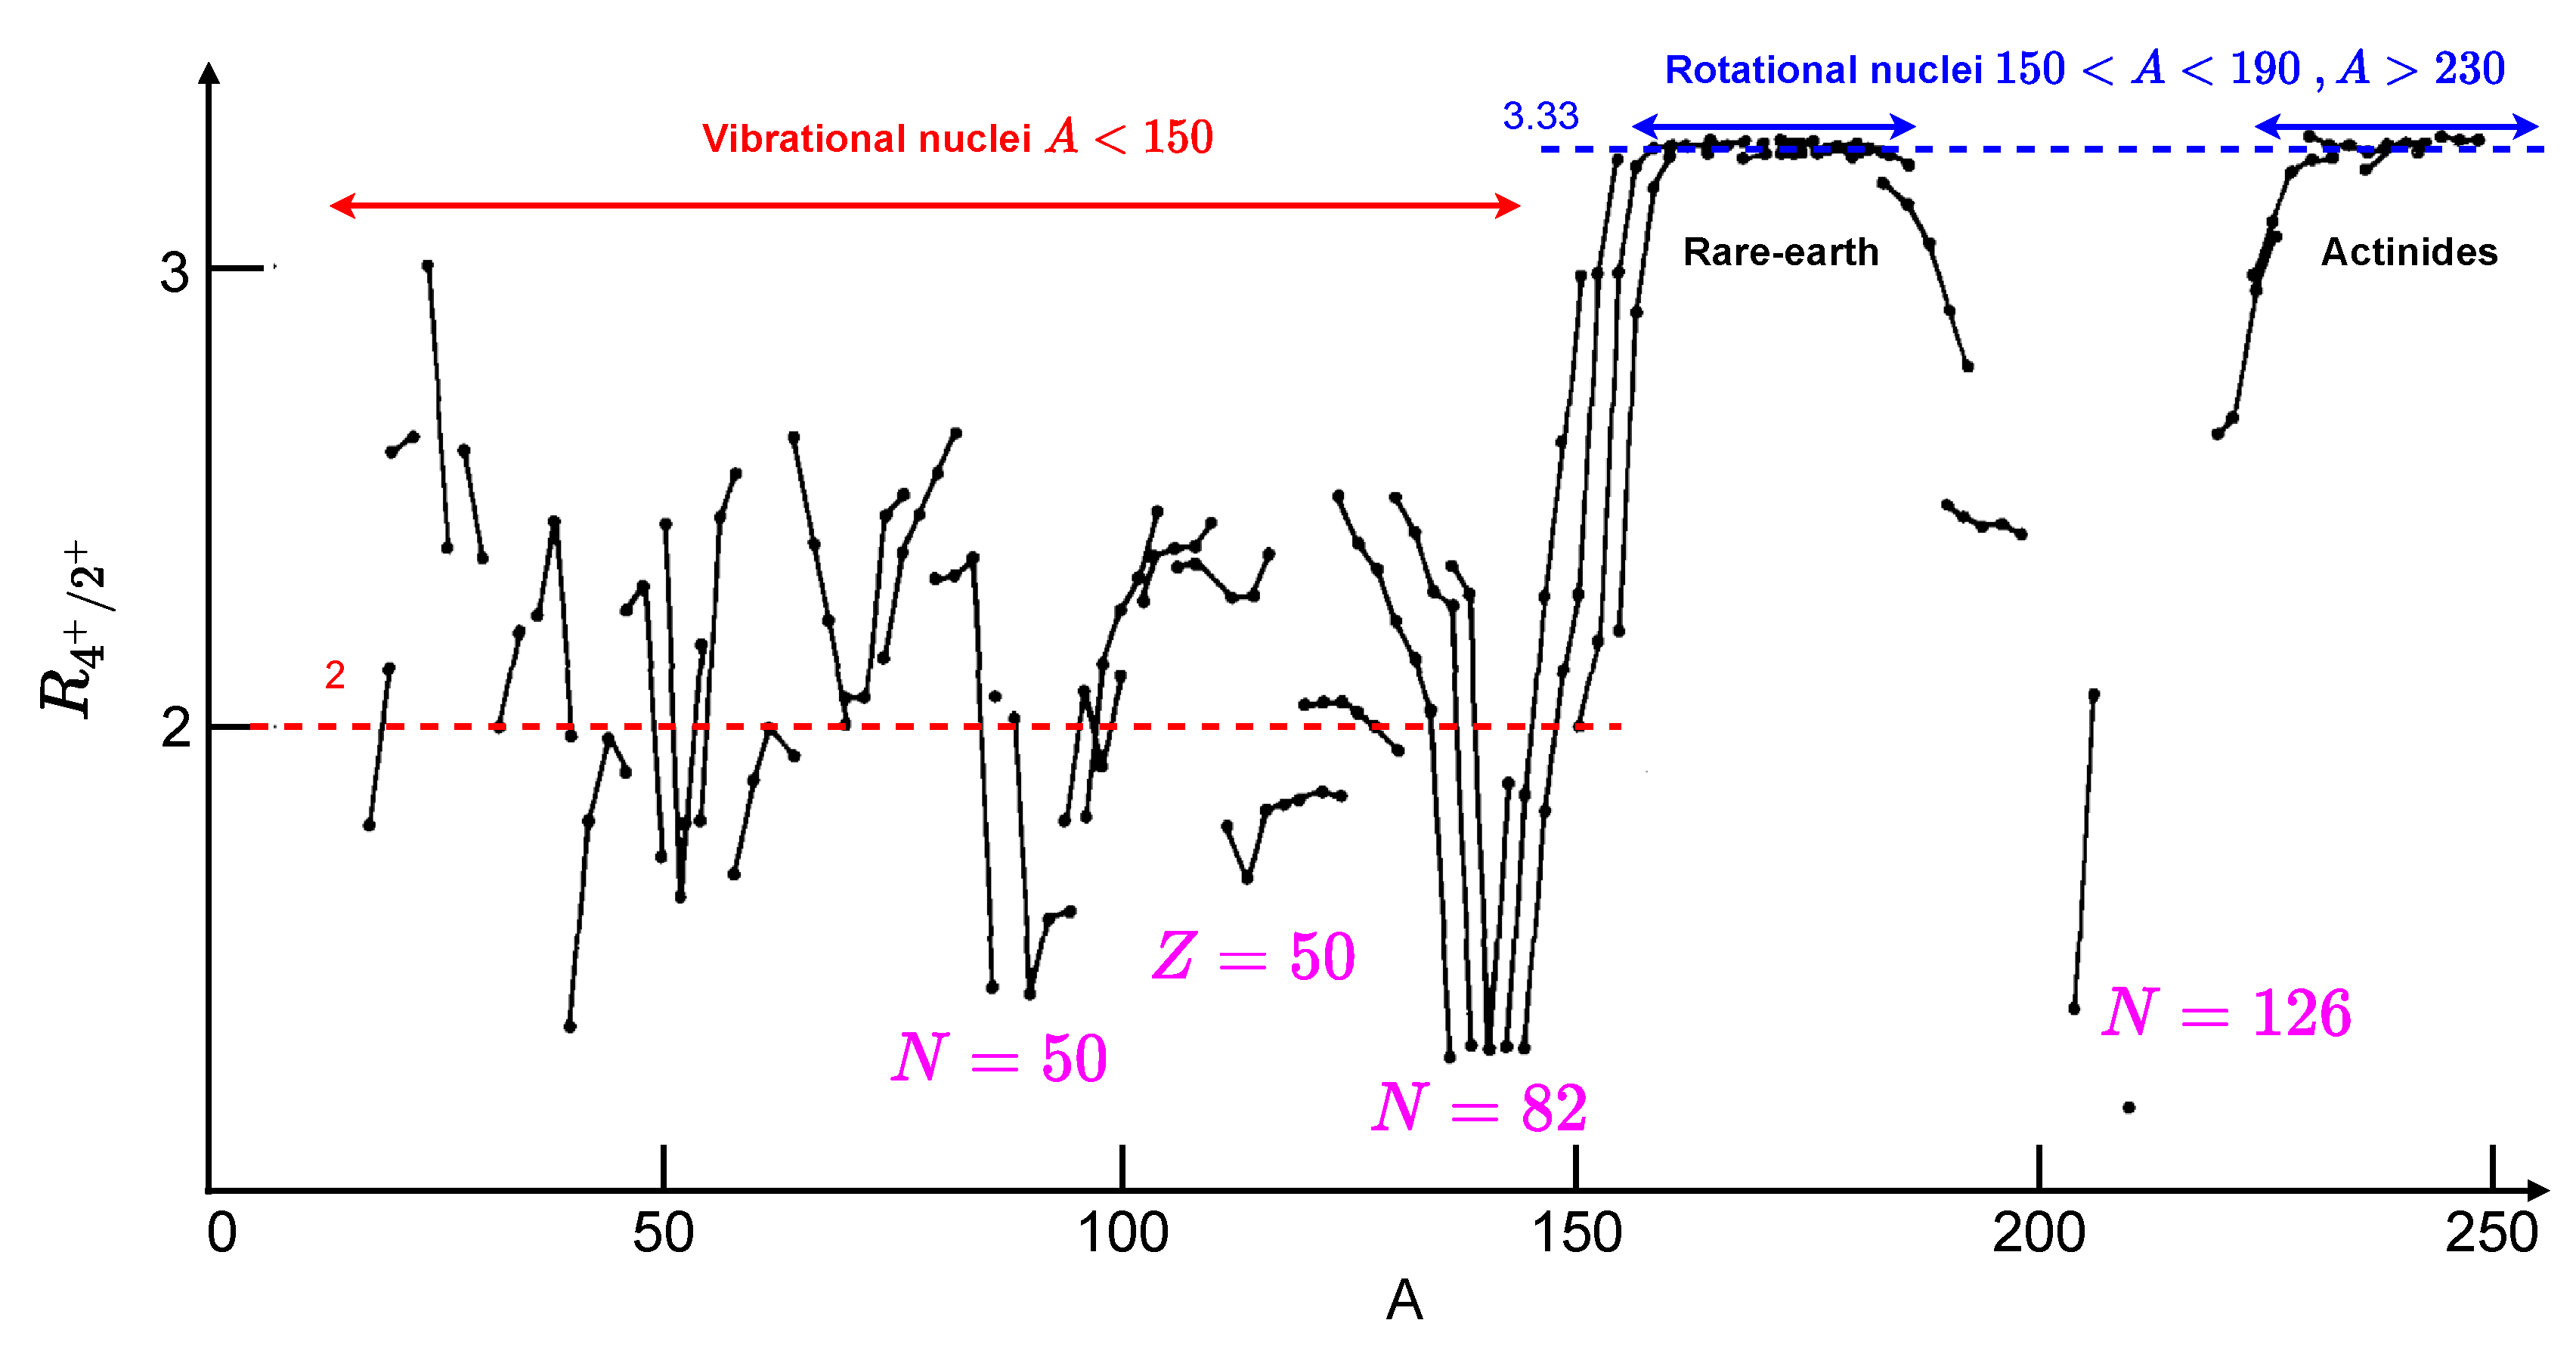
\includegraphics[scale=0.251]{Chapters/Figures/vibrations_rotations_E42-ratio.pdf}
    \caption{The experimental ratio $R_{4^+/2^+}$ in even-$Z$ and even-$N$ nuclei. Each line is connecting sequences of isotopes. Note the two important values for $R_{4^+/2^+}$, namely $2$ and $3.33$ given for a perfect vibrational nucleus and a pure rotator, respectively. Text with magenta color marks the magic numbers for $Z$ or $N$. This plot was adapted from Ref. \cite{casten2000nuclear}.}
    \label{4state-2state-ratio}
\end{figure}

\subsubsection*{Rotational frequencies}

The kinetic energy of a rotating object, in the classical limit, is described as a quadratic variation of the angular frequency (frequency of rotation around a particular direction) $\omega=l_\text{cls.}/\mathcal{I}$ in the following way:
\begin{align}
    E=\frac{1}{2}\mathcal{I}\omega^2\ ,
\end{align}
which can also be given in terms of the angular momentum $l_\text{cls.}$, such that the final energy becomes $E_\text{cls.}=l_\text{cls.}^2/(2\mathcal{I})$. Quantum mechanically, it was shown that $l^2$ is usually expressed as $\hat{l}^2_\text{quantum}=\hbar^2 I(I+1)$.

Bengtsson et al. \cite{bengtsson1979quasiparticle} calculated the so-called Routhians (single-particle energies within the rotating frame of reference) and they found a \emph {canonical relation} between the energies and rotational frequencies:
\begin{align}
    \omega=\frac{\text{d}E(I)}{\text{d}I_x}\ ,
\end{align}
where the term $I_x$ is called the \emph{aligned angular momentum}, and usually it denotes the experimental spin of every state minus a reference value (see Harris \cite{harris1965higher}). The signature property discussed previously (giving sequences with $\Delta I=2$) plays a pivotal role in determining $I_x(I)$, since the projection $K$ of the angular momentum onto the deformation axis must be taken into account:
\begin{align}
    I_x(I)=\sqrt{\left(I+\frac{1}{2}\right)^2-K^2}\ ,
    \label{aligned-angular-momentum}
\end{align}
which for the $K=0$ bands reaches the simplified form $I_x^2=(I+\frac{1}{2})^2$. The value of $K$ is typically the band-head's angular momentum \cite{bengtsson1979quasiparticle,bengtsson1984signature}. 

A more concise definition for the quantity $\omega(I)$ is related to the transition between two consecutive states $I+1\to I-1$ within a rotational band: a unique value of $\omega$ is attributed to the spin $I$, which is defined as a mean value of the two angular momenta from the corresponding transition. Such a construction will yield a set of discrete points $\omega(I)$, and one can obtain a `continuous' function $\omega(I)$ together with its inverse $I(\omega)$, thus making the term $I$ from Eq. \ref{aligned-angular-momentum} to be in fact $I(\omega)$.

The rotational frequency is used to represent many quantities which characterize collective motion and nuclear deformation. For example, representing the total angular momentum $I$ (or the aligned one $I_x$) as a function of $\Omega$ can check wether multiple bands have the same nature. Moreover, as it will be shown in the following section, representing the MOI as function of $\omega$ will also get an insight on the intrinsic structure of the nucleus and the coupling schemes involved in the occurrence of the excited spectra. Another interesting feature that is present in high-spin spectra of some nuclei is the so-called \emph{backbending} phenomena, where due to the Coriolis effect, nucleons can suffer a de-pairing, leading to their angular momentum to orient along the rotational axis, thus leading to a sharp increase in the MOI \cite{ring2004nuclear,kvasil2004backbending}. These kind of effects are correlated to high deformation, increased rotation, and change in the nucleonic alignment.

\subsubsection*{Moments of inertia}

This is a crucial quantity which describes the degree of deformation for the nucleus (rotational ellipsoid), since the asymmetry between the three MOI dictates the shape of the nuclear matter (remember discussion from Chapter \ref{chapter-2}). It was already mentioned that it is possible to retrieve an \emph{experimental} value for a moment of inertia by inferring the energy spacing between consecutive levels of a collective spectrum. A classification of types of MOI was done in Eq. \ref{eq-irrotational-rigid-mois}, where the dependence of $\mathcal{I}$ on the deformation parameters (and even the mass parameter $B_\lambda$ that originates from the initial Bohr Hamiltonian \ref{collective-hamiltonian-stiffness-inertia}) was shown.

In order to get values for MOIs from the experimental data, two quantities are required: the spins and energies of two consecutive levels within an excited spectrum. The most general expression for the MOI can be written as \cite{ahmad2021backbending}:
\begin{align}
    \mathcal{I}=\frac{\hbar^2}{2}\left(\frac{\text{d}E}{\text{d}J(J+1)}\right)^{-1}\ ,
\end{align}
where the classical angular momentum $J$ is related to its quantum equivalent via the correction $J=I+1/2$ (see Eq. \ref{aligned-angular-momentum}). Practically, the derivative can be expressed in terms of the aligned angular momentum $I_x$ defined above.

Moreover, there are two types of MOI which give information about the structure of nuclei with respect to spin: \emph{kinematic MOI} and \emph{dynamic MOI}. The kinematic MOI is given by \cite{wu1992relation}:
\begin{align}
    \mathcal{I}^{(1)}=\frac{\hbar I_x}{\omega}=\hbar^2 I_x\left(\frac{\text{d}E}{\text{d}I_x}\right)^{-1}\ .
    \label{kinematic-moi-general}
\end{align}

One can see why the aligned angular momentum is important, since its variation w.r.t. the energies lead to theoretical determinations of the kinematic MOI. From the observed intraband $E2$ transitions one can extract the (kinematic) moment of inertia via the rule:
\begin{align}
    \mathcal{I}^{(1)}(I-1)=\hbar^2\frac{2I-1}{E_\gamma(I,I-2)}\ ,
    \label{kinematic-moi-energy-levels}
\end{align}
where $E_\gamma(I,I-2)$ represents the energy difference between two consecutive levels $E(I)$ and $E(I-2)$. The dependence on $I$ for this type of MOI makes its experimental determination to require some spin assignments to each state of the excited spectrum. On the other hand, the dynamic moment of inertia is expressed as \cite{wu1992relation}:
\begin{align}
    \mathcal{I}^{(2)}(I)=\hbar\frac{\text{d}I_x}{\text{d}\omega}=\hbar^2\left(\frac{\text{d}^2E}{\text{d}I_x^2}\right)^{-1}\ ,
    \label{dynamic-moi-general}
\end{align}
while $\mathcal{I}^{(2)}$ expressed in terms of the energy differences has the following form:
\begin{align}
    \mathcal{I}^{(2)}(I)=\hbar^2\frac{4}{\Delta E_\gamma(I)}=\hbar^2\frac{4}{E_\gamma(I+2,I)-E_\gamma(I,I-2)}\ .
    \label{dynamic-moi-energy-levels}
\end{align}
Note that any calculations for the dynamical MOI does not require prior knowledge about the spin assignments of the energy states. These two types of MOI are usually represented as function of the rotational frequency $\omega$. Since the total spin $I$ can be expressed as a function of rotational frequency, plotting the kinematic/dynamic MOI as function of angular momentum is also preferred. In the present work, these quantities are of high interest (graphical representations for different nuclei will be shown in a future chapter), their relative behavior will help characterize bands with similar nucleonic structure.

An alternative description of the quantitative analysis of these MOI can be done through the so-called $ab$ formula \cite{wu1992relation,wu1992spin}, where the energies corresponding to the rotational spectrum are parametrized as: $E(I)=a\left(\sqrt{1+bI(I+1)}-1\right)$. Fitting the experimental data will produce a set of parameters $(a,b)$ that will be used to get expressions for the kinematic and dynamic MOI:
\begin{align}
    \mathcal{I}^{(1)}=\mathcal{I}_0\left[1-\frac{(\hbar\omega)^2}{a^2b}\right]^{-1/2}\ ,\\
    \mathcal{I}^{(2)}=\mathcal{I}_0\left[1-\frac{(\hbar\omega)^2}{a^2b}\right]^{-3/2}\ ,
\end{align}
with the factor $\mathcal{I}_0$ defined as the \emph{band-head} moment of inertia: $\mathcal{I}_0=\frac{\hbar^2}{ab}$. In fact, such an approach of determining the MOIs of several odd-$A$ nuclei will consist in a future work of the same team.

As mentioned, the sharp or abrupt irregularities of the MOI with respect to the increase in rotational frequency is known as backbending. The Figs. \ref{fig-hfNuclei-mois}-\ref{fig-ErYbnuclei-mois} show some experimental data in which the quantity $\frac{2\mathcal{I}}{\hbar^2}$ as function of the squared rotational frequency is graphically represented.

\begin{figure}
    \centering
    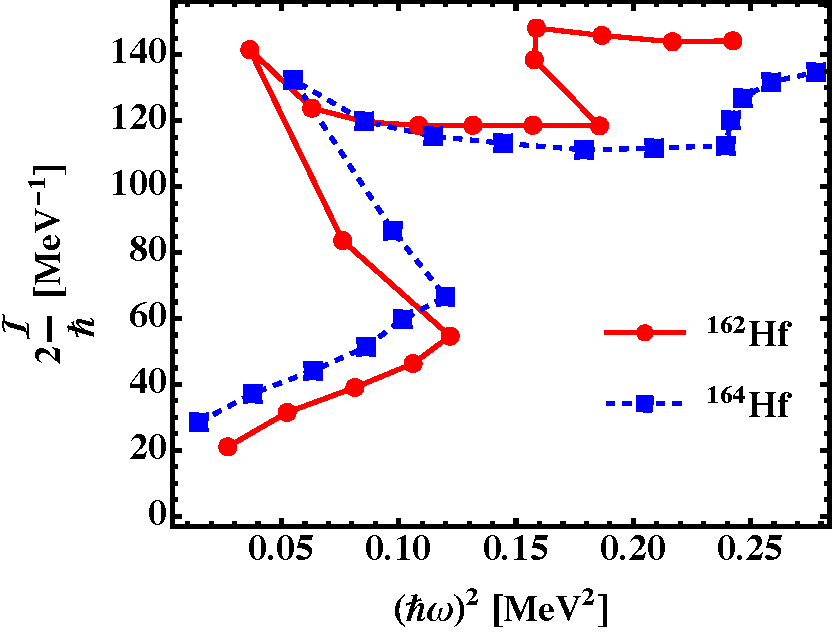
\includegraphics[scale=0.51]{Chapters/Figures/mois_Hf162-164.pdf}
    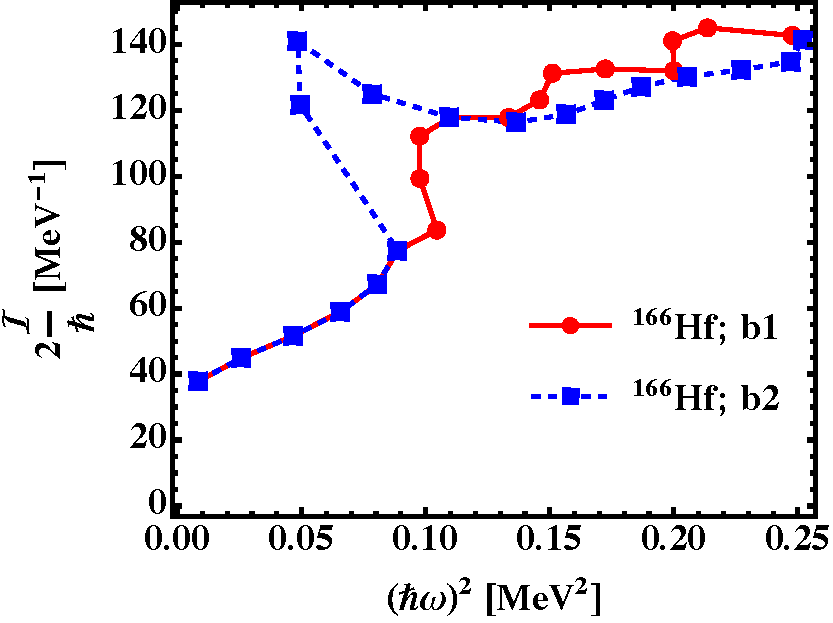
\includegraphics[scale=0.52]{Chapters/Figures/mois_Hf166.pdf}
    \caption{The moment of inertia as a function of rotational frequencies for three even-even nuclei. \textbf{Left:} The MOI for $^{162,164}$Hf nuclei, with their corresponding rotational ground-state bands. \textbf{Right:} The MOI for the first two rotational bands in $^{166}$Hf. Experimental data for these two nuclei are taken from Ahmad et al. \cite{ahmad2021backbending}.}
    \label{fig-hfNuclei-mois}
\end{figure}

\begin{figure}
    \centering
    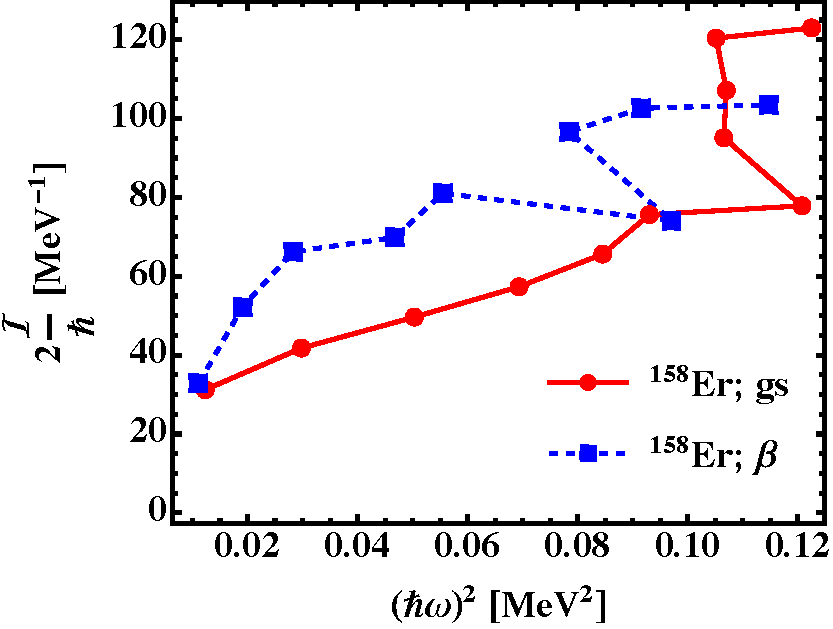
\includegraphics[scale=0.5]{Chapters/Figures/mois_Er158.pdf}
    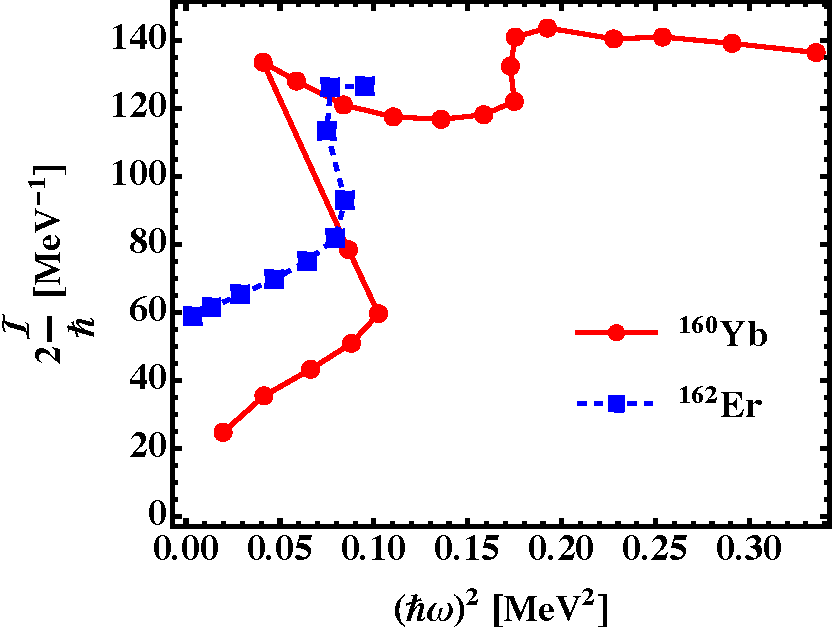
\includegraphics[scale=0.5]{Chapters/Figures/mois_Yb160Er182.pdf}
    \caption{\textbf{Left:} The MOI for $^{158}$Er nucleus, with the ground-state band $K^\pi=0^+$ and the $\beta$-vibrational band with the same quantum numbers. Experimental data taken from \cite{nica2017nuclear}. \textbf{Right:} The MOI for $^{160}$Yb compared with $^{162}$Er. Experimental data taken from \cite{nica2021nuclear} ($A=158$) and \cite{reich2007nuclear} ($A=162$).}
    \label{fig-ErYbnuclei-mois}
\end{figure}

Indeed, by looking at the evolution of $\mathcal{I}$, some sharp increases are noted, and usually these are attributed to the centrifugal stretching in the rotational model \cite{davydov1960rotation}. Moreover, the constant increase in $\mathcal{I}$ is considered to happen due to the slow and constant quenching of the pairing correlations between nucleons (as already discussed in terms of the Coriolis effect at high spin) \cite{mottelson1960effect}. The abrupt changes are explained as rapid phase transitions of the nucleonic matter \cite{krumlinde1974effect} exclusively due to the Coriolis Anti Pairing effect (example for some even-even nuclei in Ref. \cite{raduta2011semimicroscopic}).

\subsubsection*{Electric Quadrupole Moment}

One of the most important indicators of stable nuclear deformation is a large value for the \emph{electric quadrupole moment} \cite{hamamoto2016interplay}. The most general expression for the intrinsic quadrupole moment of a nucleus which is rotating about its $z$-axis is given in terms of its \emph{charge density distribution}:
\begin{align}
    Q_0=\int(3z^2-r^2)\rho(r)_\text{charge}\text{d}v\ .
\end{align}
This shows how the nuclear charge distribution inside the nucleus is a crucial indicator of deformations. Note this $z$ notation for a rotating axis is used here just for consistency with the textbook expression of $Q_0$ \cite{casten2000nuclear}. Indeed, a relationship between the deformation parameter $\beta$ and the quadrupole moment itself can be approximated (in second order of $\beta$) as:
\begin{align}
    Q_0=\frac{3}{\sqrt{5\pi}}R^2Z\beta(1+0.16\beta)\ ,
\end{align}
where $R$ is given as $R=R_0A^{1/3}$. For the $\beta$ values that correspond to proper deformed nuclei (i.e., $\beta\approx 0.3$), higher order terms are not necessary. Remember that $\beta$ describes the eccentricity of the deformed ellipsoid (albeit prolate or oblate), while the difference between prolate and oblate shapes is that for prolate (oblate) case there is an extension in one (two) direction and a squeezing in the other two (one). Depending on the value of $\beta$, the quadrupole moments for nuclei will be positive (indicating a stable prolate deformation) and negative (for stable oblate deformations). Fig. \ref{fig-quadrupole-beta-nuclides} shows some experimental values for some nuclei within the rare earth region.
\begin{figure}
    \centering
    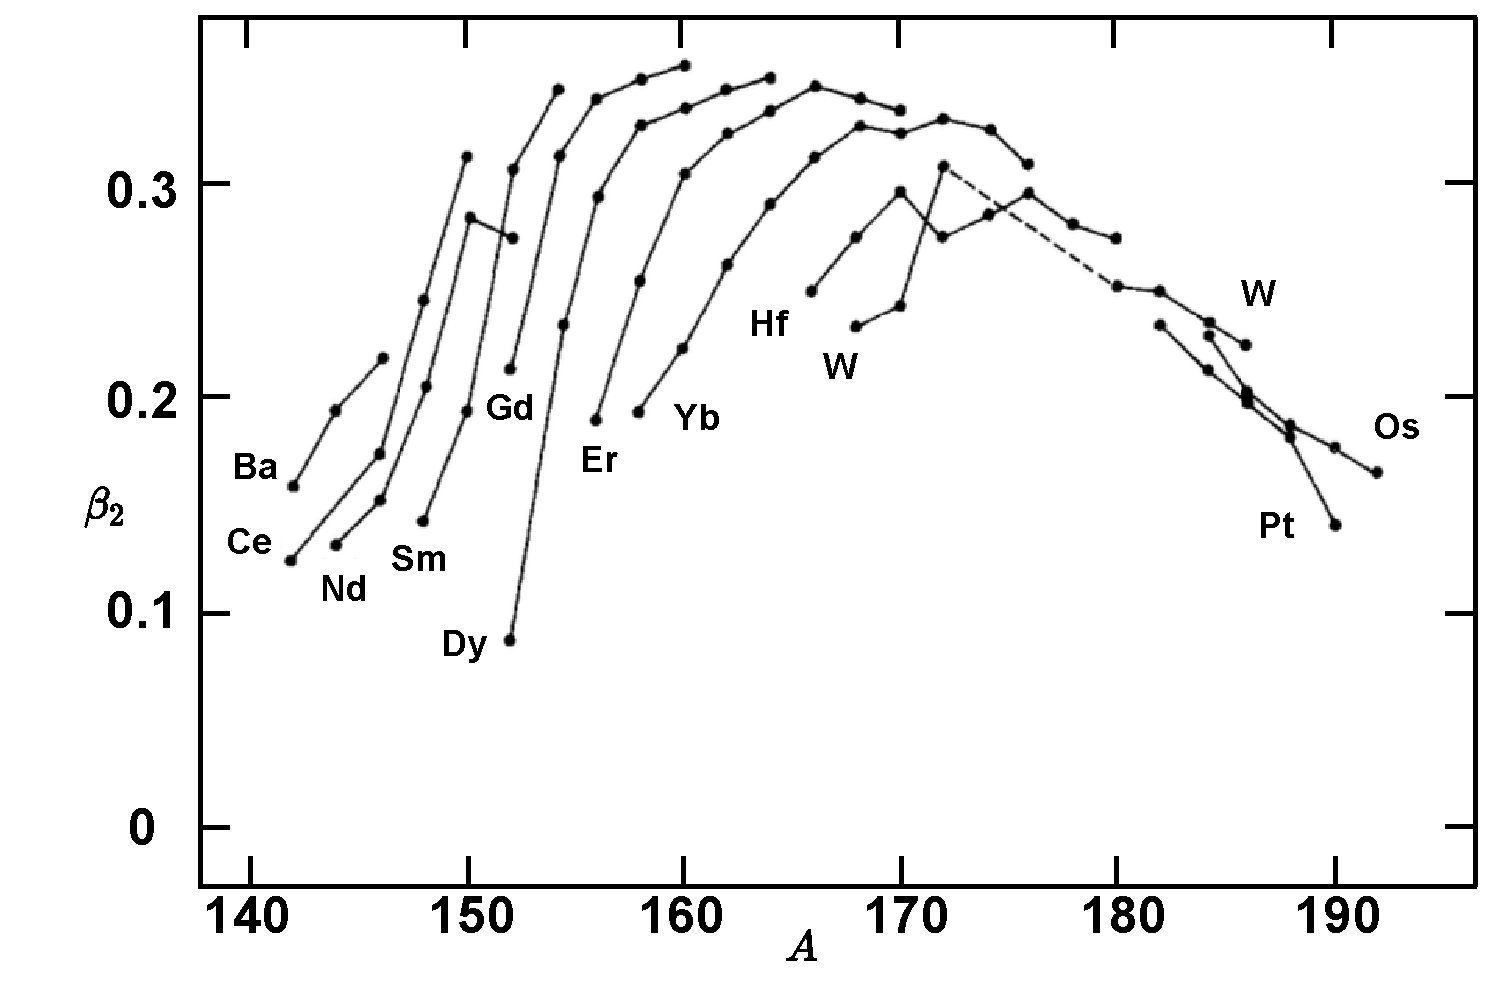
\includegraphics[scale=0.55]{Chapters/Figures/quadrupole_Deformation_rareEarth.pdf}
    \caption{Experimental values for the quadrupole deformation parameter $\beta_2$ as a function of the mass number $A$ for a few isotopes. The values of $\beta_2$ were determined from the experimental values $B(E2;0_i^+\to 0_f^+)$. Experimental data points were taken from Ref. \cite{krane1991introductory}.}
    \label{fig-quadrupole-beta-nuclides}
\end{figure}

In order to understand the behavior of $\beta$ shown in Fig. \ref{fig-quadrupole-beta-nuclides}, some shell model considerations need to be taken into account. Firstly, when deformation kicks in, the individual $j$ orbits within a major shell are nearly empty, resulting in positive values for the quadrupole moments of the nucleons from these orbits. With increasing deformation, large and positive values $Q(\beta)$ are present. Furthermore, as the shells start to fill, contributions from individual $j$ orbits to the total quadrupole moment will accumulate, making its value to decrease, vanish, and eventually becoming negative near the shell closure.

The \emph{observed} quadrupole moment (measured, also known as spectroscopic) can be obtained via a transformation to the laboratory frame applied to $Q_0$, meaning that the spectroscopic quadrupole moment has the result \cite{casten2000nuclear}:
\begin{align}
    Q_\text{spec}=Q_0\left[\frac{3K^2-I(I+1)}{(I+1)(2I+3)}\right]\ ,
    \label{quadrupole-moment-spectro}
\end{align}
where the quantum number $K$ is again the projection of $I$ onto the symmetry (deformation) axis. The dependence of $Q_\text{spec}$ on $K$ and $I$ emphasizes the fact that the \emph{observed} shape of the rotating nucleus is not equivalent to the shape in the intrinsic frame of reference.

Remarking the fact that when prolate nucleus rotates about an axis that is perpendicular to the symmetry axis, the \emph{averaged} density distribution of the nuclear matter will look more like an oblate shape (see Fig. \ref{fig-averaged-prolate-density} for a clearer picture). As a result, when the intrinsic quadrupole moment is positive, the observed one will have a negative value: for the condition $I(I+1)>3K^2$ taken from Eq. \ref{quadrupole-moment-spectro}.

\begin{figure}
    \centering
    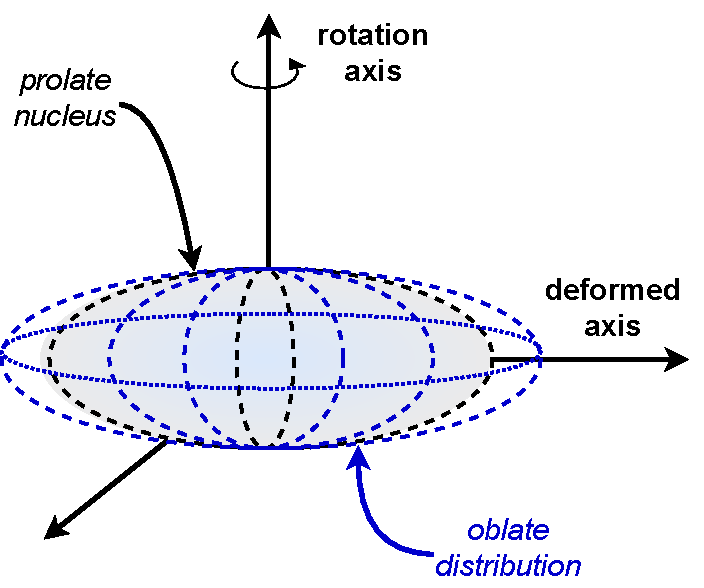
\includegraphics[scale=0.65]{Chapters/Figures/averaged_nuclearMatter_prolate.pdf}
    \caption{An example which aims at depicting an average flattened (oblate) density distribution that is generated by the rotation of a prolate nucleus. As the `initial' prolate nucleus with its nuclear density is distributed along the deformed axis exhibits rotation, the rotated shape will generate an averaged oblate disk along the rotation axis. This is why the observed quadrupole moment will have a negative sign if $Q_0>0$.}
    \label{fig-averaged-prolate-density}
\end{figure}

% The \emph{transition quadrupole moment} $Q_t$ is another quantity which can be determined from the lifetime measurement of excited states, and it is related to the intrinsic quadrupole moment via \cite{ayangeakaa2013exotic}:
% \begin{align}
%     Q_t(I+1)=\sqrt{Q_0(I)Q_0(I+2)}\ .
% \end{align}

Another important quantity that can be used as a `test' for collectivity and deformation within nuclei is the $E2$ transition probability (of electric quadrupole type). This is because the ground state of even-even nuclei is $0^+$ and the first excited state (typically $2^+$) can only decay via the electric quadrupole interaction (as $E2$ radiation \cite{casten2000nuclear}), meaning that deformation effects can be understand from these low-lying transitions. The general expression for calculating a transition `strength' is given in terms of the initial and final states \cite{matta2017exotic}:
\begin{align}
    B(E2;\ I_i\to I_f)=\frac{1}{2I_i+1}\left|\bra{\Psi_f}\left|\mathcal{M}(E2)\right|\ket{\Psi_i}\right|^2\ ,
    \label{eq-general-reduced-E2}
\end{align}
where the two wave-functions represent the initial and final state, respectively, and $\mathcal{M}(E2)$ is the quadrupole transition operator. In fact, Eq. \ref{eq-general-reduced-E2} tells that the reduced transition probabilities can be extracted from the `matrix elements' of the electric quadrupole operator. Equivalently, the reduced quadrupole transition probability $B(E2)$ can be given in terms of the Clebsch-Gordan coefficients \cite{bohr1998nuclear}:
\begin{align}
    B(E2;\ I_i\to I_f)=\frac{5}{16\pi}e^2Q_0^2\left|\bra{I_iK20}\ket{I_2K}\right|^2]\ ,
\end{align}
where the coefficient can also be written as $\bra{I_iK20}\ket{I_2K}\equiv C^{I_i2I_f}_{K0K}$. In the case of $0^+\to 2^+$, the reduced transition probability will be given by:
\begin{align}
    B(E2;\ 0^+\to 2^+)=\frac{5}{16\pi}e^2Q_0^2\ .
\end{align}

From the quadratic dependence of the intrinsic quadrupole moment on $\beta$, large values of $\beta$ that are specific to deformed nuclei ($\beta\approx 0.3$) will lead to values for $B(E2)$ which are one-two orders of magnitude higher than those specific to nearly spherical nuclei ($\beta\approx 0.05$). Such a systematic is the main cause why higher $B(E2)$ values indicate large nuclear deformations.

In nuclei, usually the valence nucleons are causing some core polarizations, which as a result will affect the `final' electric quadrupole moment. In fact, the single-particle quadrupole moment is given by the following expression:
\begin{align}
    Q_\text{sp}(j)=-\frac{2j-1}{2j+2}\frac{e_\text{eff}}{e}\langle r^2\rangle\ .
    \label{single-particle-quadrupole-moment}
\end{align}
The need for an \emph{effective charge} $e_\text{eff}$ is discussed in \cite{heyde1994nuclear}. The mean squared radius corresponds to the radial function of the nucleon within that $j$ orbital. Due to the nuclear energy being minimal (when discussing stable deformation) only if the overlap of the core with the valence particle is maximal, a particle+core interaction will produce an oblate polarization, driving the nucleus to a final oblate deformed state. The opposite is true for the hole+core coupling (see discussion made in \cite{neugart2006nuclear}).

An interesting characteristic which emerges from Eq. \ref{single-particle-quadrupole-moment} is the fact that besides even-even nuclei with $I=0$, odd-$A$ nuclei the total spin $I=\frac{1}{2}$ will be zero. The experimental data from Fig. \ref{experimental-Q-odd-nuclei} show the magnitude of $Q$ which would correspond to the value given by Eq. \ref{single-particle-quadrupole-moment}. One can see sharp increase with the nucleonic number for some nuclei (e.g., $^{175}$Lu or $^{167}$Er) but also very strong decrease to negative values (e.g., the isotope $^{123}$Sn). These alternations between positive (prolate) and negative (oblate) $Q$ values are also located near the magic numbers. Moreover, one should note that for the cases when the odd-particle is a neutron, the nucleus still exhibits a quadrupole moment that is different from zero, meaning that not only the last nucleon will be responsible for the quadrupole moment \cite{bertulani2007nuclear}.

\begin{figure}
    \centering
    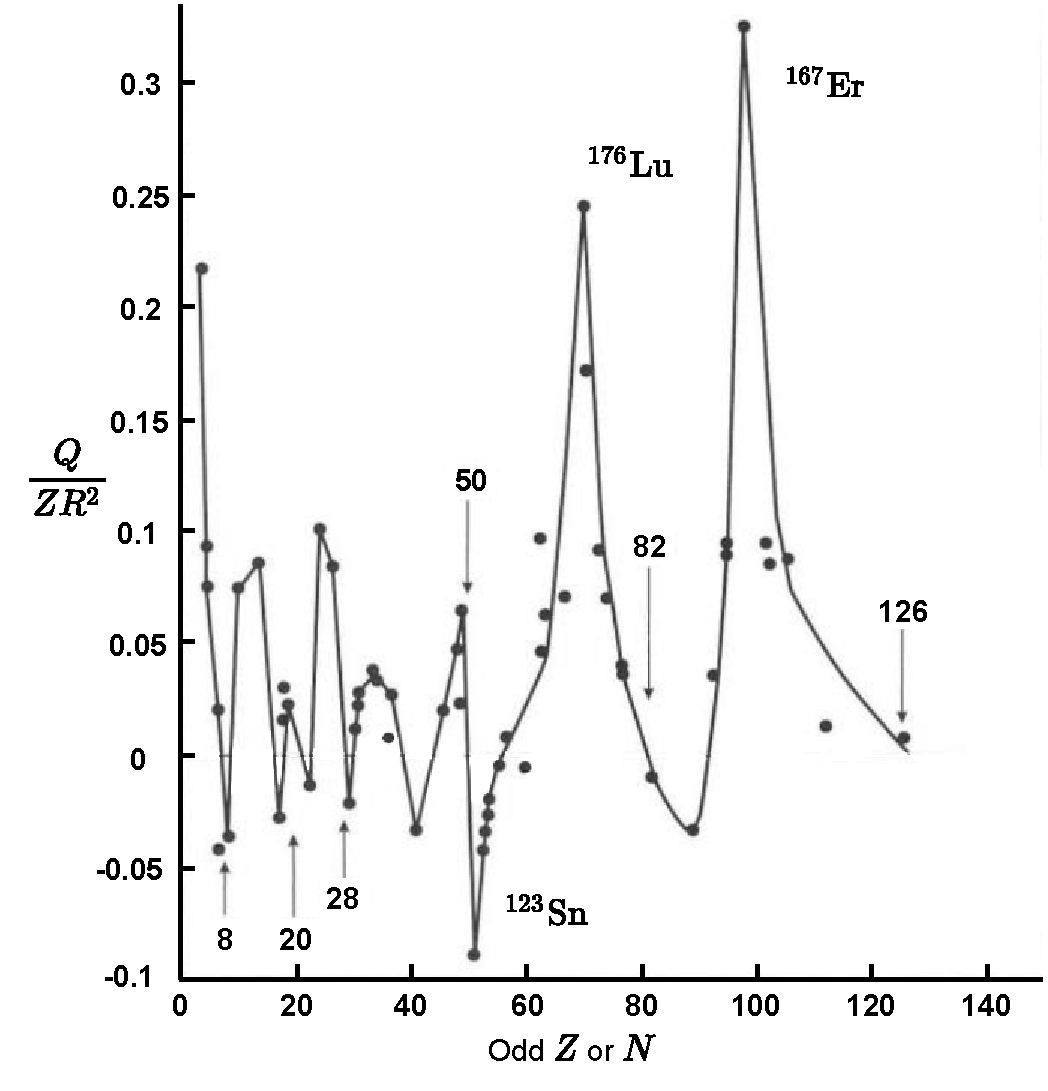
\includegraphics[scale=0.7]{Chapters/Figures/Exp_quadrupoleMoments.pdf}
    \caption{The measured quadrupole moments, given in units of $ZR^2$, as a function of the odd proton and neutron numbers $Z$,$N$, respectively. Experimental data are taken from Ref. \cite{bertulani2007nuclear}.}
    \label{experimental-Q-odd-nuclei}
\end{figure}

The experimental data for the measured $Q_\text{spec}$ values (the spectroscopic quadrupole moment in units of \emph{barn}) for the lowest $2^+$ states of even-$Z$ and even-$N$ nuclei is also graphically represented in Fig. \ref{experimental-quadrupole-2Plus-states}, where both positive and negative values are observed. As already explained, a negative value for $Q_\text{spec}$ (say for example $Q_\text{spec}=-2$ b, for nuclei with stable permanent deformation which belong to the mass range $150\leq A \leq 190$) will correspond to an intrinsic quadrupole moment $Q_0=7$ b. This will correspond to a quadrupole deformation parameter $\beta\approx 0.29$. Such values indicate substantial eccentricities of the nuclear matter.

\begin{figure}
    \centering
    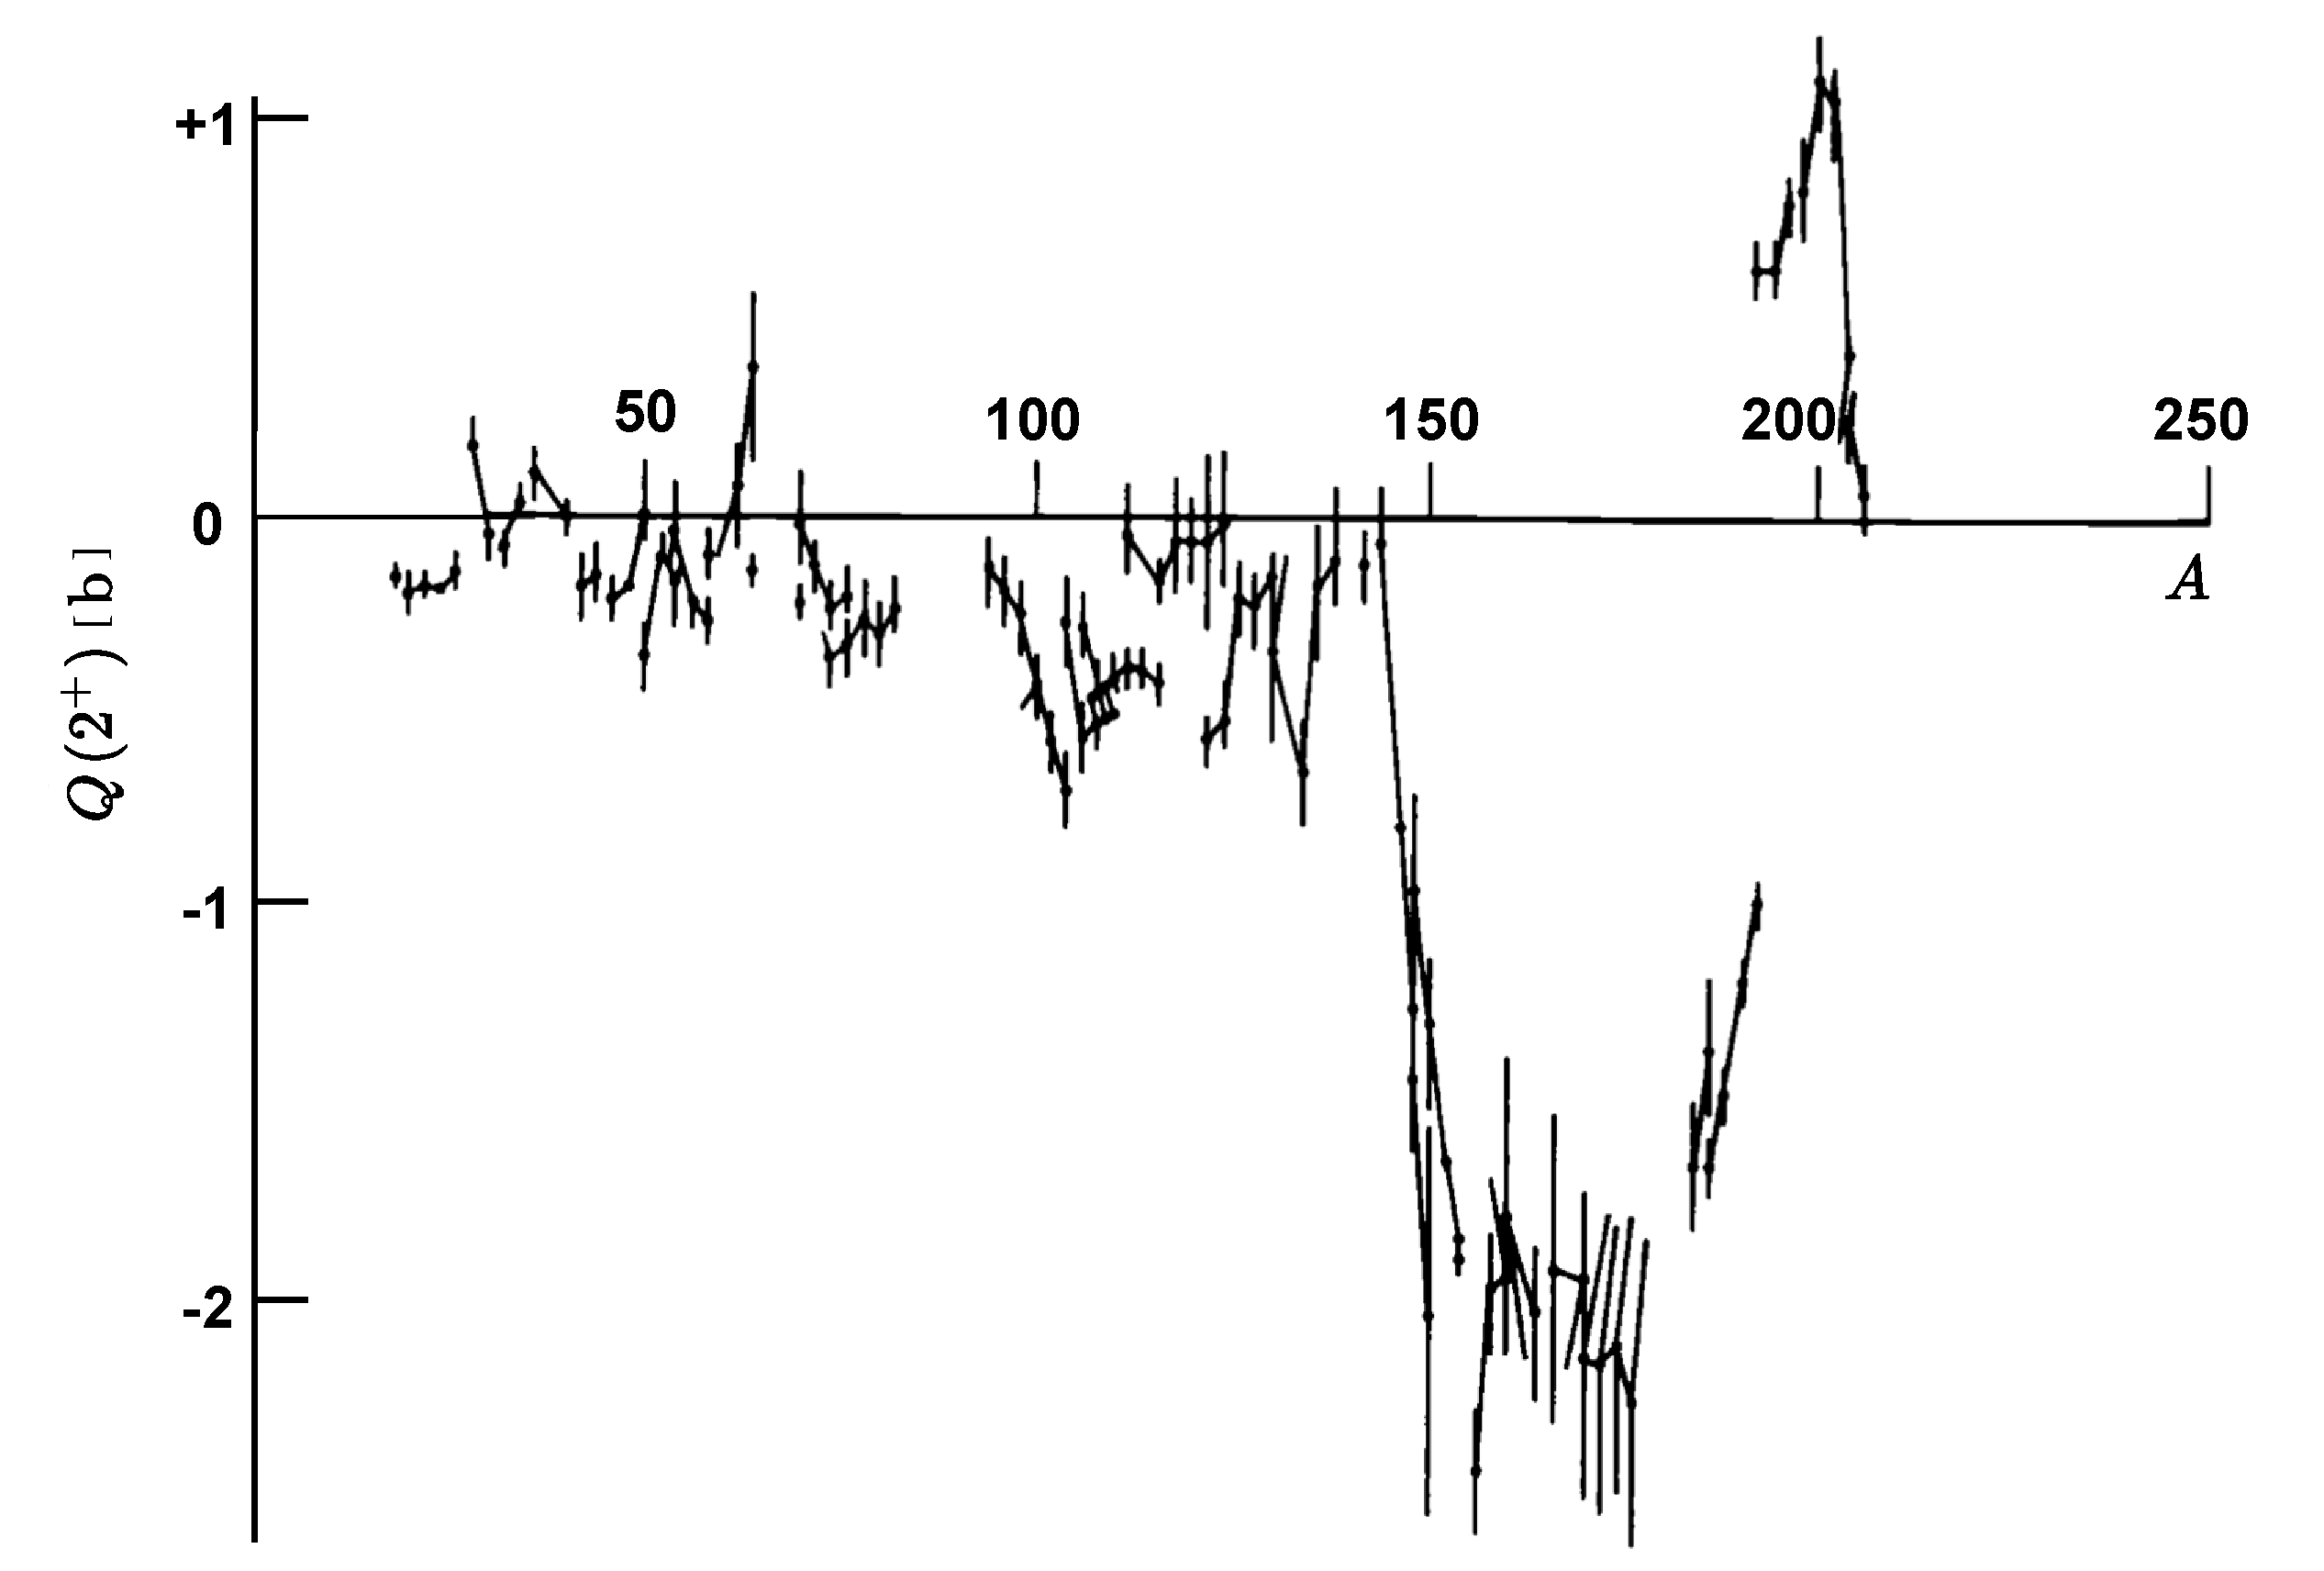
\includegraphics[scale=0.33]{Chapters/Figures/2Plus_spectroscopicQ.pdf}
    \caption{The measured quadrupole moment $Q_\text{spec}$ as defined in Eq. \ref{quadrupole-moment-spectro} for the first excited $2^+$ states in even-even nuclei. The lines between data-points connect the isotope sequences. The figure was reproduced with the experimental data from \cite{krane1991introductory}.}
    \label{experimental-quadrupole-2Plus-states}
\end{figure} % Chapter 3
\chapter{Triaxial Nuclei and Their Signatures}
\label{chapter4}
In the following chapter, some theoretical background that is necessary for understanding triaxiality will be presented, with examples from literature and also some results obtained by this team. It is also instructive to realize why the nuclear community focuses their attention to the highly deformed nuclei, and moreover, nuclei which depart so much from the spherical shapes that they become \emph{triaxial}.

Presenting the theoretical formalism that is used to describe triaxial nuclei, and mention the \emph{fingerprints} of nuclear triaxiality is that last step before diving into the recently developed framework for odd-$A$ nuclei which the team created, and showing the results. 

\section{Non-axial nuclei}

The discussion regarding excitation energies of a rigid rotator from the previous chapter was focused on pure rotators or nuclei with axially symmetric shapes (i.e,, prolate or oblate). Remember that deformation is still required in order to define a collective spectra with rotational character. Moreover, the relevant quantities that are involved in the rotational motion for a deformed nucleus are the moments of inertia corresponding to the principal axes of the deformed ellipsoid: $\mathcal{I}_{1,2,3}$, and within previous calculations, two moments of inertia were supposed to be identical.

Even though calculations are performed with the rigid-like MOI or the irrotational-like, their dependence on the deformation parameters $\beta_2$ and $\gamma$ is present (recall expressions given in Eq. \ref{eq-irrotational-rigid-mois}). Taking a closer look at their evolution with $\gamma$, one can see that indeed, identical MOI can only occur at certain values (see Fig. \ref{fig-irrotational-rigid-mois}). As such, the nuclei can be regarded (when referring to their ground state) as such:
\begin{itemize}
    \item \textbf{Spherical:} all MOI are identical and no deformations are present
    \item \textbf{Axially-symmetric:} two identical MOI and only the $\beta_2$ parameter plays a role in the collective phenomena of these nuclei
    \item \textbf{Triaxial (Axially-asymmetric):} all three MOI are different (usually one of them is very large when compared to the other two), the quadrupole deformation parameter as well as the triaxiality parameter $\gamma$ are present
\end{itemize}

Now, across the chart of nuclides, most of the isotopes are either spherical either symmetric in their ground state \cite{budaca2018tilted}, but triaxial shapes might also occur as ground-state \cite{moller2006global}. The apparition of triaxial nuclei implies some kind of `stability' on the $\gamma$-parameter, since a dynamical character of the triaxiality will indicate some transitional states rather than nuclear stability. Indeed, a rigid (fixed) value for $\gamma$ is required around the minimal region of the potential energy surface such that triaxial stable nuclei can exist. Thus, one can distinguish between the $\gamma$-soft nuclei in which this parameter has a dynamical character and the $\gamma$-rigid ones, which could in fact exhibit stable triaxial deformation \cite{dracoulis2013isomers}.
Even more interesting are the structures which occur at very large values of quadrupole deformation $\beta_2$ and $\gamma$ in the vicinity of $\approx 30^\circ$ (where maximal triaxiality occurs). It will be shown that these last nuclei will lead to band structures that are called \emph{Triaxial Strongly Deformed} bands (TSD for short) \cite{odegaard2001evidence,jensen2002evidence}.

Concluding, the triaxial nuclei are a special class of nuclei in which there is an asymmetry between the moments of inertia (given by a $\gamma$ value within the corresponding interval), and moreover, the quadrupole deformation is high enough such that it stabilizes the entire system.

\subsection{Triaxial Rotor Model}
\label{trm-model}

The most general Hamiltonian for a \emph{triaxial system} is given in terms of the components of the total angular momentum operator $\hat{I}$ and the moments of inertia for the deformed ellipsoid, similarly as it was the case for the \emph{rotational Hamiltonian} within the symmetry case:
\begin{align}
    \hat{H}=\frac{\hat{I}_1^2}{2\mathcal{I}_1}+\frac{\hat{I}_2^2}{2\mathcal{I}_2}+\frac{\hat{I}_3^2}{2\mathcal{I}_3}\ ,
\end{align}
where the indices correspond to each of the principal axes of the rotational ellipsoid (principal axes are the ones in which the components of the MOI tensor are diagonal). More often, the notations $A_{1,2,3}=\frac{\hbar^2}{2\mathcal{I}_{1,2,3}}$ are used in the Hamiltonian's expression, leading to $A_1\neq A_2\neq A_3$ for the triaxial nuclei. Shi et al. \cite{wen2015wobbling} show a very straightforward way of obtaining the eigenvalues for the \emph{triaxial rigid rotor}, following the quantum treatment made by Davydov and Filippov for the rigid rotor without symmetry axis \cite{davydov1958rotational}:
\begin{align}
    \hat{H}&=\hat{H}_\text{diag}+\hat{H}_\text{non-diag}\ ,\nonumber\\
    \hat{H}_\text{diag}&=\left[\frac{1}{2}\left(A_1+A_2\right)\left(\hat{I}^2-\hat{I}_3^2\right)+A_3\hat{I}_3^2\right]\ ,\nonumber\\
    \hat{H}_\text{non-diag}&=\frac{1}{4}\left(A_1-A_2\right)\left(\hat{I}_+^2+\hat{I}_-^2\right)\ .
\end{align}
This way of expressing the Hamiltonian is useful because there is a clear difference between a term which is diagonal and one that mixes states with different $\Delta K=\pm2$ quantum number. It is important to emphasize that this kind of Hamiltonian is still invariant to rotations with $\pi$ around the principal axes. This is useful because one can solve the eigenvalue problem with the basis $\ket{IMK}$, were the wave-function is described as:
\begin{align}
    \ket{IMK}=\sqrt{\frac{2I+1}{16\pi^2(1+\delta_{K0})}}\left[\ket{IMK}+(-)^I\ket{IM-K}\right]\ ,
\end{align}
where $\ket{IM\pm K}$ are the Wigner $D_{MK}^I$ - functions that determine the \emph{orientation} of the nucleus itself (their are functions of the three Euler angles), the $K$ quantum number is the projection of $I$ onto the 3-axis of the body-fixed frame (intrinsic frame of reference), and the $M$ number represents the projection of $I$ onto the $z$-axis of the laboratory frame. This wave-function is quite similar to the one defined in Eq. \ref{RAL-bands-wave-function}, when the decoupled states in the Rotation Aligned Bands were studied. Indeed, using this basis, the total Hamiltonian can be diagonalized \cite{wen2015wobbling} as such:
\begin{align}
    \hat{H}_{IK}=\frac{1}{2}(A_1+A_2)\left[I(I+1)-K^2\right]+A_3K^2\ ,
\end{align}
with the notation $H_{IK}\equiv\bra{IK}\hat{H}\ket{IK}$. The second, non-diagonal term will have the energy states given as:
\begin{align}
    \hat{H}_{IK\pm2}=\frac{1}{4}(A_1-A_2)\sqrt{(I\mp K)(I\pm K +1)(I \mp K -1)(I\pm K +2)}\ ,
\end{align}
where $\hat{H}_{IK\pm 2}\equiv \bra{IK}\hat{H}\ket{I\pm K}$. Finally, using these matrix elements, the energies can be obtained by solving the eigenvalue equation for given spins $I$. Such calculations were performed by the team for an even-even nucleus $^{158}$Er (see Fig. 8 from  \cite{raduta2017semiclassical}) and the results of the diagonalization procedure were in complete agreement with alternative descriptions for $\hat{H}$.

\subsection{Triaxial Particle + Rotor Model}

In this section, a general discussion about the Hamiltonian for a system which is composed on one single-particle (valence nucleon) in a high-$j$ shell and one triaxial core. Usually, such a treatment will be applied to odd-$A$ triaxial nuclei, and in fact the team's developed framework is founded on the triaxial PRM \cite{davydov1958rotational}. Davydov et al. developed this model for explaining the low-lying collective spectra of $2^+$ states within some transitional nuclei.

The Hamiltonian of this system will be composed of a term which corresponds to the even-even core and that of a single-particle which is moving in a quadrupole deformed mean-field (remember that quadrupole deformation are the only relevant effects when discussing triaxial structures).
\begin{align}
    \hat{H}=\hat{H}_\text{rot}+\hat{H}'_\text{sp}\ .
    \label{triaxial-prm-general-hamiltonian}
\end{align}

Here, an important remark must be done regarding the notation of the terms. Usually, the single-particle Hamiltonian is composed of a term that gives the \emph{intrinsic} energy coming from the $j$ shell in which the nucleon is orbiting (one can think of it as representing the Fermi energy level) and a term that characterizes the effective interaction between the particle and the deformed mean-field generated by the core. Consequently, the Hamiltonian $\hat{H}'_\text{sp}$ should be written as: $$\hat{H}'_\text{sp}=\hat{h}_0^j+\hat{H}_\text{int}^\text{quad}\ ,$$where $\hat{h}_0^j$ is the formerly described term and $\hat{H}_\text{int}^\text{quad}$ is the latter.
%the contribution of the total particle energy coming from the position of the $j$-shell and $\hat{H}_\text{int}^\text{quad}$ is the interaction of the valence nucleon with the even-even core (that is of quadrupole type). 
For example, Ring et al. \cite{ring2004nuclear} uses the SHO for describing $\hat{h}_0^j$. The interaction Hamiltonian is in fact a $\gamma$-deformed Nilsson potential, which was previously discussed (see Section \ref{nilsson-model-section}), with it's general expression in this case written as:
\begin{align}
    \hat{H}_\text{int}^\text{quad}=\kappa\beta r^2\left[\cos\gamma Y_{2}^{0}+\frac{\sin\gamma}{\sqrt{2}}\left(Y_2^2+Y_2^{-2}\right)\right].
    \label{quadrupole-deformed-potential-beta}
\end{align}
However, this generalized expression can be written for the single-particle characterized by its total angular momentum $\mathbf{j}$ in the following way:
\begin{align}
    \hat{H}_\text{int}^\text{quad}=\frac{V}{j(j+1)}\left[\cos\gamma(3j_z^2-\mathbf{j}^2)-\sqrt{3}\sin\gamma(j_x^2-j_y^2)\right]\ ,
    \label{single-particle-nilsson-defored-potential}
\end{align}
where the entire interaction strength between the particle and the core is embedded within the value of a parameter (usually adjustable) called \emph{single-particle potential strength} $V$. This parameter is very important in the present research, since the obtained theoretical results regarding energy spectra was obtained through the determination of $V$ numerically.

Peng et al. \cite{peng2003description} gave a description for nuclei within the mass region $A\approx 100,130$ using a Hamiltonian in which two valence nucleons were coupled to the triaxial core (due to the nuclear chirality arising from the odd-odd nature of nuclei). Their Hamiltonian was given as:
\begin{align}
    \hat{H}=\hat{H}_\text{intr}+\hat{H}_{coll}\ ,
\end{align}
where $\hat{H}_\text{coll}$ is the typical rotor Hamiltonian and $\hat{H}_\text{intr}$ represents the sum of a proton and neutron contribution, respectively:
\begin{align}
    \hat{H}_\text{intr}=h_p+h_n\ .
\end{align}
A remarking feature of this approach is that the problem can be extrapolated to a case with multiple protons and neutrons, invoking some sort of `scalability' of their model. Furthermore, the deformed potential (Eq. \ref{quadrupole-deformed-potential-beta}) that gives the energy splittings for the nucleonic orbits (recall the Nilsson diagrams Figs. \ref{nillson-diagram} - \ref{nillson-diagram-2}) is expressed in terms of the nucleus's mass and the quadrupole deformation parameter \cite{peng2003description}:
\begin{align}
    V_\text{int}^\text{quad}=\frac{206}{A^{1/3}}\beta_2\left[\cos\gamma Y_2^0+\frac{\sin\gamma}{\sqrt{2}}(Y_2^2+Y_2^{-2})\right]\ .
    \label{quadrupole-deformed-potential-V}
\end{align}
The single-particle energies for protons and neutrons have a somewhat similar form as the one stated in Eq. \ref{single-particle-nilsson-defored-potential}, namely it is given as:
\begin{align}
    h_{p(n)}=\pm\frac{1}{2}C_\beta\left[\left(j_3^2-\frac{j(j+1)}{3}\right)\cos\gamma+\frac{1}{2\sqrt{3}}(j_+^2+j_-^2)\sin\gamma\right]\ ,
    \label{single-particle-energies-hpn}
\end{align}
with the alternating signs corresponding to the proton and neutron, respectively. The \emph{coupling parameter} $C_\beta$ is a measure of energy (typically expressed in MeV units) and its value depends linearly on $\beta$:
\begin{align}
    C_\beta=\frac{195}{j(j+1)}\beta A^{-1/3}\ .
\end{align}
% \subsubsection*{Numerical application - Deformed Potential}
It is worth giving some quantitative results concerning the quadrupole potential and the single-particle Hamiltonian described above. As such, a simple numerical application will be employed, giving graphical representations with the behavior of these quantities with respect to the deformation parameters. Firstly, the potential $V_\text{int}^\text{quad}$ will be analyzed in the polar plane defined by the angles $(\theta,\varphi)$ which enter in the expression of the spherical harmonics. For nuclei within $A\approx 160$ region, it is common to have values of $\beta_2\approx 0.2,0.3$ and $\gamma\approx 20^\circ$, so values for these parameters will be given within this range. The quadrupole potential $V_\text{int}^\text{quad}$ can be seen in Figs. \ref{figs-deformed-quadrupole-potential-1} - \ref{figs-deformed-quadrupole-potential-2}.

\begin{figure}
    \centering
    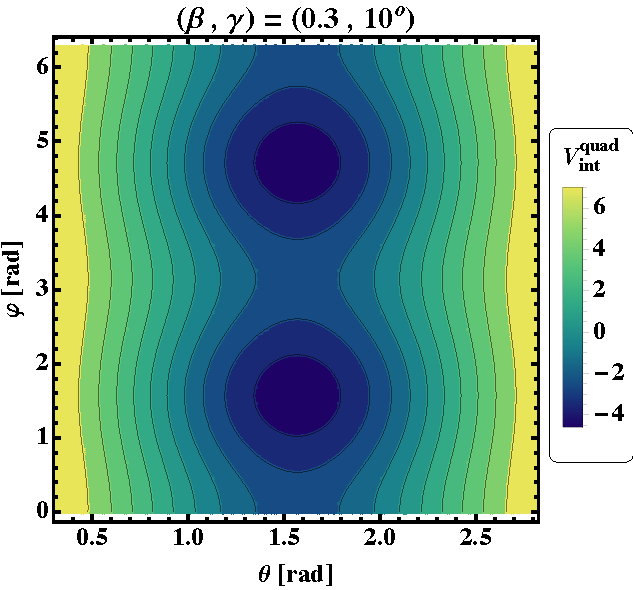
\includegraphics[scale=0.66]{Chapters/Figures/quadrupole-potentialV-1.pdf}
    \includegraphics[scale=0.66]{Chapters/Figures/quadrupole-potentialV-2.pdf}
    \caption{The quadrupole potential $V_\text{int}^\text{quad}$ as defined in Eq. \ref{quadrupole-deformed-potential-V}, represented as a function of the angular coordinates $\theta$ and $\varphi$. Calculations were done with fixed parameters $\beta_2$, $\gamma$, and for $A=163$.}
    \label{figs-deformed-quadrupole-potential-1}
\end{figure}

\begin{figure}
    \centering
    \includegraphics[scale=0.66]{Chapters/Figures/quadrupole-potentialV-3.pdf}
    \includegraphics[scale=0.66]{Chapters/Figures/quadrupole-potentialV-4.pdf}
    \caption{The quadrupole potential $V_\text{int}^\text{quad}$ as defined in Eq. \ref{quadrupole-deformed-potential-V}, represented as a function of the angular coordinates $\theta$ and $\varphi$. Calculations were done with fixed parameters $\beta_2$, $\gamma$, and for $A=163$.}
    \label{figs-deformed-quadrupole-potential-2}
\end{figure}

For the evaluation of $h$ given in Eq. \ref{single-particle-energies-hpn} (the indices $p,n$ are dismissed hereafter), one can take the diagonal components of $h$ and apply the rules only for one proton ($p$). As a result, the \emph{mixing terms} $j_+$ and $j_-$ from $h$ won't contribute at all, since their action on protonic states $\ket{jk}$ will give zero. Only the $(j_3^2-j(j+1)/3)$ term will contribute to the diagonal components of $h$. For a proton state $\ket{jk}$, where $k=-j,\dots,j$, the diagonal element $\bra{jk}h\ket{jk}$ will be:
\begin{align}
    h_{jk}\equiv\bra{jk}h\ket{jk}=\frac{1}{2}C_\beta\cos\gamma\bra{jk}\left(j_3^2-\frac{j(j+1)}{3}\right)\ket{jk}\ ,
\end{align}
which can be simplified to:
\begin{align}
    h_{jk}=\frac{1}{2}C_\beta\cos\gamma\left(k^2-\frac{j(j+1)}{3}\right)\ .
    \label{hdiag-equation}
\end{align}
This matrix elements will be functions of deformation parameters as well as the projection $k$ of the particle'
s angular momentum onto the $3$-axis. Since $j_3$ is applied twice on $\ket{jk}$ state, the final result will be $k^2$, so only the positive values can be considered for the numerical application $k=1/2,\dots,j$. When a high-$j$ proton orbital (say $h_{11/2}$ or $i_{13/2}$) is considered, for a nucleus with $A=167$, the evolution of $h_{jk}$ as function of $\beta_2$ and $\gamma$, respectively, are shown in Figs. \ref{hdiag-beta-evolution}. For completeness, the evolution w.r.t. the triaxiality parameter $\gamma$ for the diagonal matrix elements of $h$ are shown Fig. \ref{hdiag-gamma-evolution}.

\begin{figure}
    \centering
    \includegraphics[scale=0.7]{Chapters/Figures/singleParticle-hdiag-1.pdf}
    \includegraphics[scale=0.7]{Chapters/Figures/singleParticle-hdiag-2.pdf}
    \caption{The evolution with quadrupole deformation parameter $\beta_2$ for the diagonal matrix elements of $h_{jk}$ defined in Eq. \ref{hdiag-equation} (proton on a defined $j$-shell), at a fixed triaxiality parameter $\gamma$. See text for details.}
    \label{hdiag-beta-evolution}
\end{figure}

\begin{figure}
    \centering
    \includegraphics[scale=0.7]{Chapters/Figures/hdiag-gamma-1.pdf}
    \includegraphics[scale=0.7]{Chapters/Figures/hdiag-gamma-2.pdf}
    \caption{The evolution with triaxiality parameter $\gamma$ for the diagonal matrix elements of $h_{jk}$ defined in Eq. \ref{hdiag-equation} (proton on a defined $j$-shell), at a fixed deformation parameter $\beta_2$. See text for details.}
    \label{hdiag-gamma-evolution}
\end{figure}

Regarding this numerical application, one can observe the fact that since only the cosine function is present in the diagonal components of $h$, the single-particle energies are independent on the sign of $\gamma$ (since cosine is an even function). However, this is not the case when calculations are done for the non-diagonal elements, since states with different $k$ will add contributions to $h$ via the sine function. For the evolution of $h_{jk}$ with $\beta_2$, one can see that the lines in Fig. \ref{hdiag-beta-evolution} (especially the right plot) are almost similar, indicating that the diagonal components are not very sensitive to nuclear triaxiality. On the other hand, a difference in $\beta_2$ between the components will result in large gaps.

Going back to the general Hamiltonian given in Eq. \ref{triaxial-prm-general-hamiltonian} and putting together Eqs. \ref{quadrupole-deformed-potential-beta}, \ref{single-particle-nilsson-defored-potential}, \ref{quadrupole-deformed-potential-V}, it can be brought to a `final' form. With this, rotor and the single-particle contributions are clearly depicted while the influence of the quadrupole deformation and triaxiality also explicitly employed \cite{ring2004nuclear}:
\begin{align}
    % \hat{H}=\sum_i\frac{R_i^2}{2\mathcal{I}_i}+h_0^j+\kappa\beta r^2\left[\cos\gamma Y_2^0+\frac{\sin\gamma}{\sqrt{2}}\left(Y_2^2+Y_2^{-2}\right)\right]\ ,\\ 
    \hat{H}=\sum_i\frac{R_i^2}{2\mathcal{I}_i}+h_0^j+\frac{V}{j(j+1)}\left[\cos\gamma(3j_z^2-\mathbf{j}^2)-\sqrt{3}\sin\gamma(j_x^2-j_y^2)\right]\ .
    \label{eq-triaxial-prm-full-hamiltonian}
\end{align}

Regarding the dynamical character of $\hat{H}$ defined in Eq. \ref{eq-triaxial-prm-full-hamiltonian}, the coupling of high-$j$ particle with a rotor will create physical effects which can be classified in the following way \cite{ring2004nuclear}:
\begin{itemize}
    \item rotational energy is always minimized by the rotation of the core around the axis with the largest MOI
    \item alignment of the odd particle will always prefer a maximal mass overlap with the core (this configuration minimizes the potential energy the most)
    \item the Coriolis effect will always tend to align the particle with the core, in terms of their a.m.
\end{itemize}

Concluding this section, by using the triaxial PRM one can describe the energies of a an odd-$A$ triaxial nucleus, and moreover, as it will be shown, quantities such as transition probabilities (electric quadrupole type) and quadrupole moments can be calculated. It is a starting ground for multiple theoretical descriptions which aim to verify, confirm, and even predict phenomena specific to highly deformed shapes.

\section{Stable Triaxial Deformation}

As it was mentioned, across the chart of nuclides, stable isotopes do exist in an \emph{equilibrium} at which no symmetries are involved with regards to their shape. Quantitatively, the stability of a triaxial nucleus is related to the presence (existence) of minima within the \emph{Potential Energy Surface}. This energy surface characterizes the shape of the nuclear surface with respect to the deformation parameters $\beta$ and $\gamma$. One can speculate on the fact that for an ellipsoidal shape, the total energy at a fixed angular momentum, function of the deformation will be given as \cite{ring2004nuclear}:
\begin{align}
    E(\beta,\gamma,I)=E_\text{LDM}(\beta,\gamma,I)+E_\text{shell}(\beta,\gamma,I)-\bar{E}_\text{corr}(\beta,\gamma,I)\ ,
    \label{energy-surface-correction-terms}
\end{align}
where $E_\text{LDM}$ is the deformation energy for a rotating ellipsoid (characterized by the rigid-like MOI, since at high spin values this approximation holds true), $E_\text{shell}$ is the energy within the shell model (can even use the Nilsson's deformed variant), and $\bar{E}_\text{corr}$ is usually calculated as an \emph{averaged value} of the Nilsson-Strutinsky corrected potential \cite{brack1972funny} (which is beyond the scope of this work). Finding these energies can be done by working at constant $\omega$ or at constant I, when diagonalizing the deformed-single particle potential in the rotating frame \cite{ring2004nuclear}.

Solving thus Eq. \ref{energy-surface-correction-terms} results in having a \emph{qualitative} analysis for the behavior of the nucleonic matter at high spins. These `solutions' will consist of graphical representations in the $(\beta,\gamma)$-plane, where values with different magnitudes for the potential energy appear. The lower these values are, the `more stable' the deformation is. Typically, one can find regions of stability across the plane with well-defined values for $\beta$ and $\gamma$ at which nucleus is stable and deformed. On the other hand, if the energy variation is rather flat in the $\gamma$ degree of freedom, but centered around a finite $\beta$, then this nucleus is called \emph{$\gamma$-unstable}. These energy surfaces are a key indicator of stability with respect to the deformation parameters. Examples of energy surfaces for some nuclei are shown in Figs. \ref{pes-example-set-1} - \ref{pes-example-set-2}. It is remarkable the fact that small quantum fluctuations will exist around the minima.
In order to explain the theoretical implications of Figs. \ref{pes-example-set-1} - \ref{pes-example-set-2}, one needs to understand that based on a MHO, a so-called \emph{Ultimate Cranker} (UC) numerical implementation has been developed \cite{bengtsson1989method,bengtsson1990high} (a Nilsson deformed potential in which pairing interaction is taken into account). This implementation is able to give the values for $(\beta,\gamma)$ at which a nucleus might achieve stability, practically identifying local and global minima within the potential energy surface. In a future section, multiple isotopes with known stable triaxiality will be classified in terms of the deformation parameters, creating thus an `inventory' with these deformed nuclei.

\begin{figure}
    \centering
    \includegraphics[width=0.49\textwidth]{Chapters/Figures/174Hf-PES.pdf}
    \includegraphics[width=0.49\textwidth]{Chapters/Figures/even-A-PES.pdf}
    \caption{\textbf{Left:} Potential energy surface for $^{174}$Hf, evaluated at a constant rotational frequency. Positive parity and a signature $\alpha=0$ were considered. Four minima that could be attributed to known configurations are identified which are marked with red colored dots (normal deformation) and blue dots (strong deformation). This figure was taken from Ref. \cite{djongolov2003extending}. \textbf{Right:} PES for some even-even nuclei. Note the rather shallow triaxial minima for all nuclei, and the $\gamma$-soft nature of all the nuclei except for $^{106}$Pd, whose minimum is achieved at a null triaxiality parameter. This figure was taken from Ref. \cite{nomura2021examining}.}
    \label{pes-example-set-1}
\end{figure}

\begin{figure}
    \centering
    \includegraphics[scale=0.17]{Chapters/Figures/135Pr-PES.pdf}
    \includegraphics[scale=0.38]{Chapters/Figures/163Lu-PES.pdf}
    \caption{\textbf{Top:} PES for the odd-$A$ nucleus $^{135}$Pr, with units of MeV. The figure is taken from the work of Frauendorf et al. \cite{frauendorf2014transverse}. \textbf{Bottom:} PES for the odd-$A$ isotope $^{163}$ evaluated at a fixed spin $I=53/2$ with positive parity and positive signature. The red dot corresponds to a global minimum for normal deformed structure, while the blue diamonds represent two additional minima which correspond to strong deformation. This plot is taken from Ref. \cite{jensen2002wobbling}.}
    \label{pes-example-set-2}
\end{figure}

Similarly, PES calculations for other nuclei will also point out the stable deformations (with triaxial character), extracting the deformation parameters. For instance, within the $A\approx160$ mass region there are multiple nuclei in which TSD bands are identified. Best example are the results concerning Lu-Hf isotopes, where more than 20 such bands were experimentally confirmed \cite{gu2007theoretical}. It is interesting that fact that the nuclei with even $N$ (especially the Lu isotopes) have ground state TSD bands which emerge from a configuration based on the $\pi=i_{13/2}$ nucleon. In fact, Ødegård et al. \cite{odegaard2001evidence} point out the fact that nuclei with proton number $Z\approx 71$ and neutron number $N\approx 94$ have stable triaxial shapes with large quadrupole deformation around the values $(\beta_2,\gamma)=(0.38,\pm 20^\circ)$, while the lowest energy state corresponding to the odd nucleon is the $i_{13/2}$ proton \cite{schnack1995superdeformed}.

Given the degree of shell filling, only some specific triaxial shapes with fixed value of $\gamma$ are favored by the aligned particle (see Ref. \cite{hamamoto1983intrinsic} for more details). In the case of $^{163}$Lu, the aligned proton from $j=13/2$ shell favors a triaxiality of $\gamma=20^\circ$ (see Fig. \ref{pes-example-set-2}). Similarly, other nuclei will have different high-$j$ nucleon configurations which will drive the system to large triaxial deformations, by favoring a particular value of $\gamma$.

Now that the stability of asymmetric nuclear shapes has been visualized in terms of energy surfaces and deformation parameters (whose magnitudes are more or less given by the favoring of the single-particle configuration), it is instructive to understand how one can identify triaxial nuclei (both experimentally and theoretically). This will be done in the following section.

\section{Fingerprints of Triaxiality}

Within recent years, it has been shown that triaxiality plays an important role on features such as:
\begin{itemize}
    \item Calculating nucleon separation energies \cite{moller2006global}
    \item Protonic emission probabilities \cite{qi2019recent,budaca2022deformation}
    \item Determination of fission barrier height \cite{moller2009heavy,lu2012potential}
    \item Nuclear fragmentation \cite{palumbo1985splitting}
\end{itemize}

Unfortunately, triaxiality is still quite challenging to measure it directly \cite{hamamoto2016interplay,budaca2018tilted}. On the experimental side, a tremendous effort was made in order to construct setups that can study nuclei at very high spins (were collective phenomena previously discussed appear). Over the last 25 years, with the advance in technology of detectors \cite{henning2012stability}, some large facilities were built, with the sole purpose of studying high-spin nuclei with great degree of precision on the spectroscopic measurements that are performed. Facilities such as the EUROBALL \cite{simpson1997euroball} or GAMMASPHERE \cite{lee1990gammasphere} opened \emph{new frontiers} on the nuclear physics at high-spin; being able to measure excited spectra of nuclei having angular momentum within the range $60-80\hbar$. Regarding the reactions involved, most of the measurements of highly excited (and rapidly rotating) are obtained through \emph{Fusion-Evaporation Reactions} in which heavy-ion collisions take place. Since this work does not focus on the experimental setups and procedures, only some literature covering these reactions are mentioned: \cite{gu2007theoretical,henning2012stability,ayangeakaa2013exotic,matta2017exotic,das2018nuclear,lewis2019lifetime,sensharma2021wobbling}.

Even though stable triaxiality is an elusive phenomenon, \emph{two clear fingerprints} are known to pinpoint asymmetric nuclear shapes: \textbf{wobbling motion} and \textbf{chiral symmetry breaking}. There has been an extensive study of these two phenomena, and both indicate a clear correspondence between their physical significance and the lack of symmetry for the underlying nuclei. Since wobbling is the main focus of this work, a brief introduction for chiral symmetry breaking will be made below, while a separated chapter will be devoted to the theoretical and experimental evidence regarding wobbling motion. Moreover, all the theoretical results obtained within the team's framework will be presented.

\subsection{Chiral motion}

Firstly introduced by Frauendorf \cite{frauendorf1997tilted}, it concerns nuclei in which the nucleonic configurations lead to a system that lacks \emph{chiral symmetry}, meaning that the the left-handed system is not identical with its right-handed system. The left/right handedness of the nuclear system comes from the coupling of three different angular momenta, typically that is a valence proton, a valence neutron, and a rotational core (of collective nature). As such, the chiral symmetry breaking is expected to appear in odd-odd nuclei.

In this pioneering work, it was shown that for a triaxial nucleus, the collective angular momentum $\mathbf{R}$ will align along the intermediate ($i$) axis of the deformed ellipsoid (note that the $i$-axis is also the axis with largest MOI). Regarding the particles, the location of their corresponding Fermi level will dictate the alignment of the nucleons with the ellipsoid \cite{frauendorf1997tilted,starosta2001chiral}. For a valence proton with the energy located in the bottom part of the high-$j$ subshell, it will align its a.m. with the short $s$-axis of the ellipsoid. Furthermore, a valence neutron having located in the upper part of the high-$j$ shell will align its a.m. with the long $l$-axis. Reasoning for these kind of orientations have been discussed already: they are related to the overlap between the single-particle wave-functions and that of the triaxial nuclear shape. \emph{Maximal overlap will always minimize the interaction energy}. The three alignments will result in a perpendicular set of a.m., so they can be arranged in configurations with different chirality: left- and right-handed systems. The chiral operator combines a rotation with the time-reversal operator: $\chi_\text{chiral}=\mathcal{T}R_y(\pi)$.

When the chiral symmetry is broken in the intrinsic frame of reference (body-fixed frame), the `restoration' of the symmetry in the laboratory frame will manifest itself as the emergence of two almost degenerate doublet bands with $\Delta I=1\hbar$ \cite{frauendorf1997tilted}. Also, in the laboratory frame of reference, this pair of bands will appear since the symmetry (broken in the body-fixed frame) will be restored via the quantum tunneling effect \cite{zhang2007chiral}. This interesting behavior has been drawing a lot of attention lately, with most of the experimental identifications around the transitional nuclei $A\approx 130$. Great research towards complete spectroscopy of some chiral nuclei has been done in Refs. \cite{starosta2001chiral,meng2008chiral,budaca2018tilted,budaca2018semiclassical,budaca2021chiral}. Examples of experimental chiral doublets are shown in Figs. \ref{chiral-bands-1} - \ref{chiral-bands-2} for some odd-odd nuclei.

\begin{figure}
    \centering
    \includegraphics[width=0.99\textwidth]{Chapters/Figures/Chiral_136Pm.pdf}
    \caption{The energy spectra for the odd-odd $^{136}$Pm isotope, in which the chiral doublet built on the configuration $\pi h_{11/2}\otimes\nu h_{11/2}$ appears. Experimental data is from Ref. \cite{mccutchan2018nuclear} and the level scheme is adapted from Ref. \cite{bhat1992evaluated}.}
    \label{chiral-bands-1}
\end{figure}

\begin{figure}
    \centering
    \includegraphics[scale=0.7]{Chapters/Figures/chiral_bands_132La.pdf}
    \caption{The energy spectra for the odd-odd $^{132}$La isotope, in which the chiral doublet built on the configuration $\pi h_{11/2}\otimes\nu h_{11/2}$ appears, with each double being properly colored in red and blue, respectively. Experimental data is taken from from Ref. \cite{grodner2004dsam,grodner2005lifetime}.}
    \label{chiral-bands-2}
\end{figure}

The geometrical interpretation of the left-handed and right-handed systems can be seen in Fig. \ref{chiral-geometry}, where the ellipsoid is `surrounded' by the two valence nucleons, each with its aligned a.m. w.r.t. principal axes.

\begin{figure}
    \centering
    % \includegraphics[width=0.99\textwidth]{Chapters/Figures/chiral_handedness-1.pdf}
    % \includegraphics[width=0.99\textwidth]{Chapters/Figures/chiral_handedness-2.pdf}}
    % \includegraphics[width=0.49\textwidth]{Chapters/Figures/chiral_handedness_v2-LH.pdf}
    % \includegraphics[width=0.49\textwidth]{Chapters/Figures/chiral_handedness_v2-RH.pdf}
    \includegraphics[width=0.99\textwidth]{Chapters/Figures/chiral_handedness.pdf}
    \caption{Left- and right-handed chiral systems for a triaxial odd-odd nucleus, indicating the mutually perpendicular angular momentum vectors. The two valence nucleons with their orbits are colored with blue (proton) and magenta (neutron). These figures were inspired from \cite{starosta2001chiral}. Considering the discussion regarding alignments, the proton a.m. $\mathbf{j}_\pi$ is aligned with the $s$-axis, the neutron a.m. $\mathbf{j}_\nu$ with the $l$-axis, and the even-even core a.m. $\mathbf{R}$ with the $m$-axis of the ellipsoid. The coupling scheme is described in text.}
    \label{chiral-geometry}
\end{figure}

\section{Wobbling Motion}

The second fingerprint of triaxiality is the `core' topic of this work, and it will be discussed in detail in the next chapter, where some theoretical ideas will be presented together with the latest experimental results. A great amount of progress towards understanding nuclear phenomena at high spin has been made by the scientific community which devoted research to this particular topic.

Going back to the discussion about the triaxial shapes and their asymmetry between the MOI, this key feature leads to the possibility of defining a rotation about any of the three axis. Although the main rotational motion will be around the axis with the largest MOI (since this is energetically the cheapest \cite{bohr1954rotational}), the other two axes will contribute to a `total' (superimposed) rotation such that the angular momentum $\mathbf{I}$ of the system will precess around a steady position. The precessional motion has oscillator-like behavior, meaning that $\mathbf{I}$ will not only precess, but its projection around the principal axes will oscillate around a steady position.
The easiest way of understanding wobbling motion is a classical analog such as the \emph{spinning asymmetric top}, but for a nucleus the spinning motion is \emph{quantized} and a typical phonon number will be attributed to the system.

As it will be shown in the following chapter, treating the wobbling phenomenon in a `classical' will lead to very good results concerning the physical quantities of interest. Moreover, there are many attempts (albeit quantum mechanical or semi-classical approximations) at describing wobbling motion in which the parameters used to describe the Hamiltonian have clear analogies with quantities that describe classical systems, keeping thus a close contact with well-defined concepts regarding system dynamics.

Other classical analogies for the nuclear wobbling motion can be seen in celestial bodies such as planets. Indeed, Earth has a precession given by its rotation and a small amplitude polar motion. As a result, the Earth's `angular momentum' will oscillate with respect to one of the body's fixed axis.
 % Chapter 4
\chapter{Wobbling Motion in Nuclei}

The pioneering work of Bohr and Mottelson \cite{bohr1998nuclear} which was done more than 50 years ago lead to some interesting features regarding the collective phenomena in triaxial nuclei. Namely, they pointed out that a specific precessional motion of the nucleus's spin will take place when the rotational energy is sufficient. The angular momentum for triaxial nuclei is not aligned any of the principal axes of the ellipsoid, but it \emph{precesses} and \emph{wobbles} around one of these axes. They called this phenomenon \textbf{wobbling motion} (w.m.).
This combined motion comes from a consequence regarding the MOI. Indeed, the asymmetry of the three MOI makes the quantum mechanical nature of rotation to be possible around any of the three axes. As such, a \emph{main} rotation around the axis with the largest MOI will be the most energetically favorable, but the other two directions can \emph{quantum mechanically disturb} this main rotation, leading to this unique characteristic of triaxial nuclei.

The non-uniformity nature of w.m. was firstly studied for the `pure' rigid-rotators that correspond to the even-even nuclei. In this case, the w.m. can be treated as small amplitude oscillations of the total angular momentum $\mathbf{I}$ around the axis corresponding to the largest MOI.

\section{Wobbling Motion in Even-Even Nuclei}

The analytical expressions for wobbling excitations were firstly evaluated by Bohr and Mottelson using the so-called \emph{Harmonic Approximation} (HA). This can be described as a small-amplitude limit for the Triaxial Rigid Rotor Hamiltonian that was discussed in Chapter \ref{chapter4} (see Section \ref{trm-model}). In this limit, the projection of the total angular momentum onto the axis with largest MOI can be approximated $I_3\approx I$, meaning that the nucleus will do most of its rotation around this axis, with some `disturbance' from the other two principal of the triaxial rotor. 

For the description of this simple wobbler, one can consider the case when the $3$-axis has the largest MOI, and the following order holds true:
\begin{align}
    \mathcal{I}_3>\mathcal{I}_2>\mathcal{I}_1\ ,
\end{align}
or equivalently:
\begin{align}
    A_3<A_2<A_1\ .
\end{align}
The Hamiltonian can be written as:
\begin{align}
    \hat{H}_\text{rot}={\color{red}A_3I_3^2}+{\color{blue}\left(A_1I_1^2+A_2I_2^2\right)}
    \label{general-rotor-ham-evenA}
\end{align}

The different colors from Eq. \ref{general-rotor-ham-evenA} try to emphasize the fact that a Hamiltonian for the simple wobbler can be regarded as \emph{a main rotation around $3$-axis} (represented by red color) and \emph{the (precession + oscillation) of the total angular momentum} (represented by blue color).

The wobbling excitations which cause oscillations with small amplitudes for $\mathbf{I}$ about the $3$-axis are assumed to have a harmonic-like behavior, meaning that the final energy spectrum of a simple wobbler (even-even nucleus) will have the typical $\hbar\omega(n+1/2)$ behavior. Since this oscillator motion can be explained as `vibrations' of the total angular momentum around a steady position, where each wobbling excitation consists of an additional vibrating phonon, one can express the Hamiltonian in terms of \emph{boson} creation and annihilation operators. As such, the quantum mechanical treatment implies \cite{bohr1998nuclear}:
\begin{align}
    b^\dagger=\frac{1}{\sqrt{2I}}I_+\ ,\ b=\frac{1}{\sqrt{2I}}I_-\ ,\ \left[b,b^\dagger\right]\approx 1\ .
\end{align}

This initial quantization allows one to write Eq. \ref{general-rotor-ham-evenA} as a rotational term and a wobbling-specific one:
\begin{align}
    \hat{H}_\text{rot}&={\color{red}A_3I_3^2}+{\color{blue}H_w}\ ,\label{rot-ham-non-diagonal} \\
    {\color{blue}H_w}&={\color{blue}t_1\left(n+\frac{1}{2}\right)+\frac{1}{2}t_2(b^\dagger b^\dagger + bb)}\ ,
    \label{wob-ham-non-diagonal}
\end{align}
where the \emph{number of boson excitations} is denoted by $n$ and it is given by $n=b^\dagger b$. Each wobbling quanta will carry an angular momentum of one unit less with respect to the $3$-axis. The two factors $t_{1,2}$ are expressed in terms of the inertial parameters as \cite{bohr1998nuclear}:
\begin{align}
    t_1&=I(A_2+A_1-2A_3)\ , \\
    t_2&=I(A_2-A_1)\ .
\end{align}

Notice the linear dependence of the two parameters on the total angular momentum $I$. Moreover, depending on the values of $A_k$, the contribution of $t_{1,2}$ can be negative. Their behavior is shown within the right inset of Fig. \ref{fig-even-even-wobbling-energies}. Although the Hamiltonian $H_w$ is considered to have an oscillator-like behavior, its general expression does not look like a typical harmonic Hamiltonian. For this, the Hamiltonian given in Eq. \ref{wob-ham-non-diagonal} can be brought to a diagonalized form by introducing a new set of boson creation and annihilation operators. These operators will be written as linear combinations of $(b^\dagger,b)$:
\begin{align}
    c^\dagger=w_1b^\dagger-w_2b\ ,\\
    c=w_1b-w_2b^\dagger\ ,
\end{align}
where the two coefficients $w_{1,2}$ are defined in terms of $t_{1,2}$ as:
\begin{align}
    w_1&=\left[\frac{1}{2}\left(\frac{t_1}{\sqrt{t_1^2-t_2^2}}+1\right)\right]^{1/2}\ ,\nonumber\\
    w_2&=\left[\frac{1}{2}\left(\frac{t_1}{\sqrt{t_1^2-t_2^2}}-1\right)\right]^{1/2}\ .
    \label{eqs-w1-w2-terms-wobbling}
\end{align}

The terms $w_{1,2}$ verify the condition $w_1^2-w_2^2=1$ and they make the `dangerous' products ($b^\dagger b^\dagger$,$bb$) disappear in this new representation \cite{oi2006semi}. Note that there is no spin dependence inferred in Eq. \ref{eqs-w1-w2-terms-wobbling} such that $w_{1,2}$ are constant functions of spin, unlike the coefficients $t_{1,2}$. Moreover, introducing a number operator $\hat{n}=c^\dagger c$ and the excitation quanta $\hbar\omega_w$ defined as:
\begin{align}
    \hbar\omega_w=\sqrt{t_1^2-t_2^2}=2I\sqrt{(A_1-A_3)(A_2-A_3)}\ ,
    \label{wobbling-frequency-even-A}
\end{align}
then a final expression of $H_w$ can be expressed, which has a behavior typical to the \emph{harmonic oscillator}:
\begin{align}
    H_w=\hbar\omega_w\left(\hat{n}+\frac{1}{2}\right)\ .
    \label{wob-ham-diagonal}
\end{align}

In this expression, the excitation quanta $\hbar\omega_w$ which was defined in Eq. \ref{wobbling-frequency-even-A} in terms of $t_{1,2}$ is called \emph{wobbling frequency} and its increasing linearly with the total angular momentum. Accordingly, Eq. \ref{rot-ham-non-diagonal} can be re-written with the wobbling Hamiltonian defined in Eq. \ref{wob-ham-diagonal}:
\begin{align}
    \hat{H}_\text{rot}=A_3I(I+1)+\hbar\omega_w\left(\hat{n}+\frac{1}{2}\right)\ .
    \label{rot-wob-ham-diagonal}
\end{align}

Thus, in the HA, the eigenvalues of the rotor Hamiltonian can be expressed in terms of a \emph{wobbling phonon number} $n_w$ (which is the eigenvalue of the number operator $\hat{n}=c^\dagger c$) and a \emph{wobbling frequency} (defined in Eq. \ref{wobbling-frequency-even-A}):
\begin{align}
    E_{I,n}={\color{red}A_3I(I+1)}+{\color{blue}\hbar\omega_w\left(n_w+\frac{1}{2}\right)}\ .
    \label{eq-wobbling-energy-evenA}
\end{align}

The spectrum for an even-even wobbling nucleus is thus represented by Eq. \ref{eq-wobbling-energy-evenA}. Notice again the two colored terms that illustrate the energy coming from the rotation around the $3$-axis and the disturbed motion with small oscillations around the other two axes. Consequently, the wobbling character of the system will be generated by the latter harmonic term. The wobbling phonon number $n_w$ is related to the `strength' of the tilting for $\mathbf{I}$, indicating the fact that an increasing number for $n_w$ will result in oscillations with larger amplitudes around the other two axes. The phonon number takes values $n_w=0,1,\dots$. In inset $b)$ from Fig. \ref{wobbling-geometry-tilting-sketch}, a sketch which shows the tilting effect that the wobbling phonon number has on the total angular momentum vector is drawn. For completeness, the collective structure of two wobbling bands generated through phonon excitations is exemplified in inset $a)$ from Fig. \ref{wobbling-geometry-tilting-sketch}.

\begin{figure}
    \centering
    \includegraphics[scale=0.72]{Chapters/Figures/wobbling_n_schematic-1.pdf}
    \includegraphics[scale=0.6]{Chapters/Figures/wobbling_n_schematic-2.pdf}
    \caption{\textbf{Left:} A typical wobbling structure for even-even nuclei. The yrast band contains even values of spins since the band has signature $\alpha=0$, while the first excited band has odd spins and $\alpha=1$. The intraband states differ by 2 units of angular momenta, while the interband ones differ with only one unit. \textbf{Right:} The increase of tilting angle between the rotational axis (the $3$-axis in this case) and the total angular momentum $\mathbf{I}$. With each wobbling phonon number, the total angular momentum tilts more and more, generating a `stronger' precessional motion (illustrated by the colored ellipses).}
    \label{wobbling-geometry-tilting-sketch}    
\end{figure}

An alternative way of depicting the wobbling term $H_w$ from Eq. \ref{rot-ham-non-diagonal} would be to express it more generally, in terms of $I_2$ and $I_3$. When doing so, one achieves the following form (assuming that rotation is around the $3$-axis) \cite{oi2006semi}:
\begin{align}
    % H_w={\color{magenta}(A_1-A_3)I_1^2}+{\color{orange}(A_2-A_3)I_2^2}={\color{magenta}T_\text{kin}}+{\color{orange}T_\text{pot}}\ ,
    H_w=(A_1-A_3)I_1^2+(A_2-A_3)I_2^2=T_\text{kin}+T_\text{pot}\ ,
\end{align}
where according to Ref. \cite{wen2015wobbling}, one can regard these two factors as a \emph{kinetic} and a \emph{potential} term. This way of expressing $H_w$ is instructive since it keeps a close contact with the `classical' picture of understanding the total energy of a system.

As a quantitative analysis of the wobbling frequency and the rotor energy, one can take three arbitrary values for the moments of inertia (and, implicitly, the inertia factors $A_k$) and see the behavior of both $E_{I,n}$ and $\hbar\omega_w$ with increasing angular momentum and wobbling phonon number. Keep in mind that depending on the value of the wobbling phonon number, different spin sequences will be allowed. More precisely, from the invariance of the rotor w.r.t. rotations by $\pi$ about the principal axes for even-even nuclei, the signature quantum number $\alpha$ can take the values 0 and 1. Each wobbling band will have an alternating signature, starting with $\alpha=0$ for $n_w=0$ then $\alpha=1$ for $n_w=1$ and so on: even spin sequences appear for even values of $n_w$ and odd spin sequences appear for odd values of $n_w$ (see Fig. \ref{fig-even-even-wobbling-energies}).

The rotor energy from Eq. \ref{eq-wobbling-energy-evenA} is graphically represented for an arbitrary set of moments of inertia as a function of the nuclear angular momentum $I$ in Fig. \ref{fig-even-even-wobbling-energies}. This pedagogical example contains rotational bands up to $n_w=5$ in the wobbling phonon number. From Fig. \ref{fig-even-even-wobbling-energies}, one can see the linear dependence on the total angular momentum and, moreover, the wobbling energy and frequency both are increasing with spin.

\begin{figure}
    \centering
    \includegraphics[scale=0.7]{Chapters/Figures/wobbling-evenA.pdf}
    \includegraphics[scale=0.74]{Chapters/Figures/wobblingFreq-evenA.pdf}
    \caption{\textbf{Left:} The energy spectrum for an even-even nucleus with three different moments of inertia, with the main rotation around the $3$-axis, according to Eq. \ref{eq-wobbling-energy-evenA}. Each wobbling band has alternating signature number $\alpha$ (starting with $\alpha=0$ for the ground state $n_w=0$ band). Notice the even/odd spin sequences for each band. \textbf{Right:}: The wobbling frequency plotted together with the linear terms $t_1$ and $t_2$ that are used to express $\hbar\omega_w$. Same set of MOI were used across both figures and the unit for $\mathcal{I}_i$ is $\hbar^2\ \text{MeV}^{-1}$.}
    \label{fig-even-even-wobbling-energies}
\end{figure}


Another instructive analysis would be the evolution of the components of $\mathbf{I}$ as functions of the polar and azimuthal angles $\theta,\varphi$. Indeed, expressing the three angular momentum components as:
\begin{align}
    I_1&=I'\sin\theta\cos\varphi\ ,\\
    I_2&=I'\sin\theta\sin\varphi\ ,\\
    I_3&=I'\cos\theta\ ,
    \label{angular-momentum-polar-components}
\end{align}
where $I'=\sqrt{I(I+1)}$, one can make a graphical representation for them, by letting $\theta$ and $\varphi$ vary within their corresponding intervals. In Fig. \ref{figs-angular-momentum-components-polar}, the quantities $I_1$ and $I_2$ are represented in the $(\theta,\varphi)$ plane for a fixed spin value $I=10\hbar$. Since the third component is independent of the azimuthal angle $\varphi$, it has been dismissed.

\begin{figure}
    \centering
    \includegraphics[scale=0.66]{Chapters/Figures/angular_components-TRM-1.pdf}
    \includegraphics[scale=0.66]{Chapters/Figures/angular_components-TRM-2.pdf}
    \caption{The geometrical representation of the first and second component of the total angular momentum $\mathbf{I}$ as functions of the polar angles, according to Eq. \ref{angular-momentum-polar-components}.}
    \label{figs-angular-momentum-components-polar}
\end{figure}

The other relevant observables that can be calculated for simple wobbler within the HA are the two quadrupole moments $Q_{20,22}$ and the intraband + interband $B(E2)$ transition probabilities. The quadrupole components are expressed in terms of the intrinsic quadrupole moment $Q_0$ and the triaxiality parameter as \cite{shoji2006microscopic}:
\begin{align}
    Q_{20}=Q_0\cos\gamma\ ,\ Q_{22}=\frac{1}{\sqrt{2}}Q_0\sin\gamma\ .
    \label{quadrupole-components-q20-q22}
\end{align}

These components can be furthermore used to determine the intraband $B(E2)$ transition probabilities \cite{wen2015wobbling}:
\begin{align}
    B(E2;(n,I)\to(n,I-2))=\frac{5}{16\pi}Q_{22}^2\ ,
    \label{intraband-probability-simple-wobbler}
\end{align}
and also the interband transitions:
\begin{align}
    B(E2;(n,I)\to(n-1,I-1))&=\frac{5}{16\pi}\frac{n}{I}\left(\sqrt{3}Q_{20}w_1+\sqrt{2}Q_{22}w_2\right)^2\ , \label{interband-probability-simple-wobbler-1}\\
    B(E2;(n,I)\to(n+1,I-1))&=\frac{5}{16\pi}\frac{n+1}{I}\left(\sqrt{3}Q_{20}w_2+\sqrt{2}Q_{22}w_1\right)^2\ .
    \label{interband-probability-simple-wobbler-2}
\end{align}

Notice that for the intraband transitions, going from the state $I$ to $I-2$ will only depend in a quadratic manner on the quadrupole component $Q_{22}$, making thus the transitions spin-independent.

\subsubsection*{Triaxial rotor energy vs. wobbling energy}

An important discussion should be made regarding the nomenclature for energies when referring to wobbling motion. As shown in Eq. \ref{eq-wobbling-energy-evenA}, the energy spectrum for a simple wobbler can be determined for every phonon number and spin sequences. However, that is the `full' spectrum  of the wobbler, which is composed of the \emph{yrast} states with $n_w=0$ and the \emph{excited states} having $n_w=1,\dots$ and so on. On the other hand, the so-called \emph{wobbling energies} are defined in terms of these `absolute values' (i.e., $E_{I,n}$) with the following rules \cite{wen2015wobbling}:
\begin{align}
    E_\text{wob}(I_\text{even})&=E_{I,n}-E_{I,0}\ ,\\
    % E_\text{wob}(I_\text{even})&=E_{I,n}-E_{I,0}\ ,\nonumber \\
    E_\text{wob}(I_\text{odd})&=E_{I,n}-\frac{1}{2}\left(E_{I-1,0}+E_{I+1,0}\right)\ ,
    \label{eq-wobbling-energy-definition-evenA}
\end{align}
where the former wobbling energy corresponds to the even values of $I$ and the latter is applied for odd values of $I$. Very often within literature the energies calculated via Eq. \ref{eq-wobbling-energy-evenA} are referred to also as wobbling energies, which is not the same as Eq. \ref{eq-wobbling-energy-definition-evenA}, so a distinction should be made clear.

\subsection{Testing the Harmonic Approximation}
\label{ba-130-numerical-calculations}

It is worth going further and apply the HA formalism for even-even nuclei for an existing spectrum. As such, one can take $^{130}$Ba as a testing example. As it will be discussed in a follow-up section, it turns out that experimental observations for wobbling structures in even-mass isotopes have been very scarce. Nevertheless, very recently, Petrache et al. identified a large collection of band structures in $^{130}$Ba \cite{petrache2019diversity}. Two of them are reported to be of wobbling nature \cite{chen2019transverse}. Having these two collective bands, one can check if the energy formula given in Eq. \ref{eq-wobbling-energy-evenA} for the simple wobbler can be applied for this isotope.

The method described in here will be based on a \emph{fitting procedure}, namely a set of parameters will be extracted from the expression of $E_{I,n}$ and they will be adjusted such that the experimental data is best reproduced by the theoretical model. This kind of approach works really well for `well-behaved' model functions and if the input data is large enough to reach a good fit precision. More often than not, if the model function contains parameters which have a clear physical meaning, then fitting becomes a suitable approach. In fact, in the following chapters, the developed formalism will verify the experimental data through similar fitting procedures (although their `core'-implementation will be more complex).

Looking at the energy formula from Eq. \ref{eq-wobbling-energy-evenA}, at a first glance, two fitting parameters would appear, namely the largest moment of inertia $\mathcal{I}_3$ and the wobbling frequency $\hbar\omega$. However, the wobbling frequency is furthermore dependent on the other two moments of inertia (as per Eq. \ref{wobbling-frequency-even-A}), meaning that one can use the set $\mathcal{P}_\text{fit}=\left[\mathcal{I}_1,\mathcal{I}_2,\mathcal{I}_3\right]$ as appropriate fitting parameters. The wobbling phonon number $n_w$ is attributed as follows: $n_w=0$ for the yrast band (denoted throughout calculations with B1) and $n_w=1$ for the first excited band (denoted with B2). The band B1 has signature $\alpha=0$ so it is the even-spin sequence, while B2 has odd spins. The experimental data regarding spins and energies for the two bands correspond to the measurements done in Ref. \cite{petrache2019diversity}.

\subsubsection{Energy Spectrum}

Indeed, by following the procedure described above, the set $\mathcal{P}_\text{fit}$ is obtained. The parameters, i.e., the three moments of inertia are shown in Table \ref{table-params-ba130}. Remarking that fact that the largest MOI which was obtained via the fitting procedure is the one corresponding to the $3$-axis. With these parameters, the theoretical energies are determined numerically and the two bands are compared to the measured data in Fig. \ref{plot-ba130-excitation-energies}. Concerning the fitted energies, in the present calculations, instead of working with the `absolute energies' (i.e., the exact values of the energies that correspond to the measured spectrum), the \emph{excitation energies} were used instead \cite{raduta2017semiclassical,raduta2018wobbling,raduta2020towards}. These are determined by subtracting the band-head energy of B1 (the $10^+$ level) from each excited state of B1 and B2. Doing this improves the accuracy of the results. The excitation energy for a spin state $I$ is given as:
\begin{align}
    E(I)=E_\text{abs}(I)-E_\text{abs}(I_0)\ ,
    \label{excitation-energy-general-formula}
\end{align}
where `abs.' signifies the absolute value for $E$ at that particular spin state and $I_0$ is the band-head state within the yrast band.

\begin{table}
    \centering
    \resizebox{0.35\textwidth}{!}{%
    \begin{tabular}{|cccc|}
    \hline
    \multicolumn{4}{|c|}{$\mathcal{P}_\text{fit}$}                                                                                                                        \\ \hline
    \multicolumn{1}{|c|}{$\mathcal{I}_1$} & \multicolumn{1}{c|}{$\mathcal{I}_3$} & \multicolumn{1}{c|}{$\mathcal{I}_2$} & \multicolumn{1}{c|}{Unit}                     \\ \hline
    \multicolumn{1}{|c|}{27}                & \multicolumn{1}{c|}{22}                & \multicolumn{1}{c|}{43}                & \multicolumn{1}{c|}{$\hbar^2\text{MeV}^{-1}$} \\ \hline
    \end{tabular}%
    }
    \caption{The parameter set $\mathcal{P}_\text{fit}$ obtained from the fitting procedure of the excitation energies of the two wobbling bands (B1 and B2) for $^{130}$Ba. The model function corresponds to the energy of a simple wobbler (see Eq. \ref{eq-wobbling-energy-evenA}).}
    \label{table-params-ba130}
\end{table}

\begin{figure}
    \centering
    \includegraphics[width=0.46\textwidth]{Chapters/Figures/ba130-band1.pdf}
    \includegraphics[width=0.46\textwidth]{Chapters/Figures/ba130-band2.pdf}
    \caption{Comparison between the experimental and theoretical excitation energies (Eq. \ref{excitation-energy-general-formula}) for the two wobbling bands of $^{130}$Ba (B1 and B2). Experimental data are taken from Ref. \cite{petrache2019diversity}. The theoretical data was obtained by fitting Eq. \ref{eq-wobbling-energy-evenA} as described in text, with the parameters defined in Table \ref{table-params-ba130}. Note that the band-head $I^\pi=10^+$ state from B1 is missing from the spectrum, since it was subtracted from each level.}
    \label{plot-ba130-excitation-energies}
\end{figure}

Besides the excited spectrum obtained in Fig. \ref{plot-ba130-excitation-energies}, other quantities such as the rotational frequencies for the two bands in $^{130}$Ba are compared with experimental values in Fig. \ref{wobbling-energies-130ba-expVSth}, and the obtained results agree with the measured data quite well. Note that both frequencies are increasing functions of angular momentum, although for B1, at spin $I\geq 24\hbar$, there seems to be a less of an increase, which is not fully reproduced by the fitted values. Moreover, having the excitation energies for the two bands, one can evaluate the theoretical wobbling energies as defined in Eq. \ref{eq-wobbling-energy-definition-evenA} and compare them with the experimental values. The two quantities are graphically represented in Fig. \ref{wobbling-energies-130ba-expVSth}. Remarking the fact that there is an opposite behavior for the two curves, namely the experimental wobbling energies decrease with angular momentum, while the theoretical ones are constantly increasing. Unfortunately, it turns out that by using the Hamiltonian for a \emph{simple wobbler} is not enough to completely describe the collective motion in this isotope.

\begin{figure}
    \centering
    \includegraphics[scale=0.73]{Chapters/Figures/ba130-wobbling-energies.pdf}
    \includegraphics[scale=0.7]{Chapters/Figures/ba130-rotational-frequencies.pdf}
    \caption{\textbf{Left:} The wobbling energies for $^{130}$Ba calculated with Eq. \ref{eq-wobbling-energy-definition-evenA}. For the first state of B2, the energy was determined as $E_\text{wob}(11^+)=E_\text{B2}(11^+)-\frac{1}{2}E_\text{B1}(12^+)$ since the band-head state of B1 is zero (as per the definition of excitation energy given in Eq. \ref{excitation-energy-general-formula}). \textbf{Right:} The rotational frequencies for the two wobbling bands of $^{130}$Ba, calculated using Eq. \ref{rotational-frequency-canonical}.}
    \label{wobbling-energies-130ba-expVSth}
\end{figure}

\subsubsection{Transition Probabilities}

Another step regarding the calculations for $^{130}$Ba consists of the electromagnetic transition probabilities. For this investigation some prior quantities are required. Firstly, the reduced transition probabilities $B(E2)$ (both the interband and the intraband) depend on the components $Q_{20}$ and $Q_{22}$ of the quadrupole moment. These two can be evaluated numerically using the expressions from Eq. \ref{quadrupole-components-q20-q22}, while the intrinsic quadrupole moment is furthermore evaluated using Eq. \ref{quadrupole-moment-Q0}. From the microscopic calculations performed by Chen et al. in Ref. \cite{chen2019transverse}, they determined that this isotope has a stable triaxial minimum located at $(\beta_2,\gamma)=(0.24,21.5^\circ)$. Within the following computations, this set of deformation parameters will be used. Taking the value of $\beta_2=0.24$, the intrinsic quadrupole moment $Q_0$ is readily obtained from Eq. \ref{quadrupole-moment-Q0}. The transition probabilities from Eqs. \ref{intraband-probability-simple-wobbler}, \ref{interband-probability-simple-wobbler-1}, and \ref{interband-probability-simple-wobbler-2} also depend on the two factors $w_{1,2}$ defined in Eq. \ref{eqs-w1-w2-terms-wobbling}, which are functions of the three moments of inertia. Thus, the quality of the fitting procedure will also reflect the calculus for the transition probabilities through $\mathcal{P}_\text{fit}$. The numerical values for $Q_0$, $w_{1,2}$, and $Q_{20,22}$ are presented in Table \ref{transition-parameters-ba130}. Having the deformation parameters, the $w_{1,2}$ terms, and the quadrupole components, one can evaluate the reduced transition probabilities. 

\begin{table}
    \centering
    \begin{tabular}{|c|c|c|}
    % \begin{tabular}{|p{0.15\linewidth}|p{0.25\linewidth}|p{0.5\linewidth}|}
    \hline
    Parameters & Calculated values & Observations                                               \\ \hline
    $\beta_2$  & 0.24              & Taken from Ref. \cite{chen2019transverse}                 \\ \hline
    $\gamma$   & $21.4^\circ$      & Taken from Ref. \cite{chen2019transverse}                 \\ \hline
    $w_1$      & 1.008             & Evaluated with $\mathcal{P}_\text{fit}$                    \\ \hline
    $w_2$      & 0.132             & Evaluated with $\mathcal{P}_\text{fit}$                    \\ \hline
    $Q_0$      & 390.376 $eb\cdot10^{-2}$      & As per Eq. \ref{quadrupole-moment-Q0}                                                           \\ \hline
    $Q_{20}$   & 363.213 $eb\cdot10^{-2}$          & As per Eq. \ref{quadrupole-components-q20-q22}                                                            \\ \hline
    $Q_{22}$   & 101.168 $eb\cdot10^{-2}$           & As per Eq. \ref{quadrupole-components-q20-q22}                                                            \\ \hline
    $B(E2)_\text{in}$ &        0.0509 $(eb)^2$          & Eq. \ref{intraband-probability-simple-wobbler}              \\ \hline
    \end{tabular}%
    \caption{The numerical values for the quantities which are required to determine the quadrupole transition probabilities $B(E2)$ defined in Eqs. \ref{intraband-probability-simple-wobbler} - \ref{interband-probability-simple-wobbler-2}. The parameter set $\mathcal{P}_\text{fit}$ was obtained through the fitting procedure and the values are shown in Table \ref{table-params-ba130}. The intraband transition probabilities $B(E2)$ are evaluated for states $(n,I)\to(,,I-2)$.}
    \label{transition-parameters-ba130}
\end{table}

The graphical representation from Fig. \ref{BE2out-transitions-130ba} shows the interband transition probabilities $B(E2)_\text{out}$ for states $(n_w=1,I)\to(n_w=0,I-1)$. These values are determined with the parameters defined in Table \ref{transition-parameters-ba130}. A constant decrease with spin can be observed, and an overall agreement with theoretical calculations from Ref. \cite{chen2019transverse} is observed (see inset $a$ from Fig. 4).

\begin{figure}
    \centering
    \includegraphics[scale=0.7]{Chapters/Figures/BE2-out-130Ba.pdf}
    \caption{The interband quadrupole transition probabilities (Eq. \ref{interband-probability-simple-wobbler-1}) from the first excited wobbling band (B2) to the yrast band (B1) for $^{130}$Ba.}
    \label{BE2out-transitions-130ba}
\end{figure}

Considering the interband transitions $B(E2)_\text{out}$ calculated above and the constant value for $B(E2)_\text{in}$ (typical for the HA), the ratios $B(E2)_\text{out}/B(E2)_\text{in}$ can also be evaluated. These values are good indicators if a nucleus has a strong deformation and for a wobbler, they lie within $0.2-0.5$. In Table \ref{BE2-out-in-ratio-130Ba}, the obtained ratios are compared with the experimental ones, where a decent agreement can be seen. The theoretical values are decreasing with spin.

\begin{table}
    \centering
    \begin{tabular}{|c|cc|}
    \hline
    \multirow{2}{*}{$I$} & \multicolumn{2}{c|}{$\frac{B(E2)_\text{out}}{B(E2)_\text{in}}$} \\ \cline{2-3} 
                         & \multicolumn{1}{c|}{Experimental}          & Calculated         \\ \hline
    11                   & \multicolumn{1}{c|}{}                      & 0.37           \\ \hline
    13                   & \multicolumn{1}{c|}{0.32}                  & 0.32           \\ \hline
    15                   & \multicolumn{1}{c|}{0.36}                  & 0.27           \\ \hline
    17                   & \multicolumn{1}{c|}{0.22}                  & 0.24           \\ \hline
    19                   & \multicolumn{1}{c|}{0.22}                  & 0.21           \\ \hline
    21                   & \multicolumn{1}{c|}{0.41}                  & 0.19           \\ \hline
    23                   & \multicolumn{1}{c|}{}                      & 0.18           \\ \hline
    25                   & \multicolumn{1}{c|}{}                      & 0.16           \\ \hline
    \end{tabular}%
    \caption{The ratios $\frac{B(E2)_\text{out}}{B(E2)_\text{in}}$ for $^{130}$Ba. The interband transitions signify the change from a state $I$ in B2 to a state $I-1$ in B1. The experimental data (where available) was taken from Ref. \cite{petrache2019diversity,chen2019transverse}.}
    \label{BE2-out-in-ratio-130Ba}
\end{table}

\subsubsection{General Discussion}

Even though the spectrum of this even-even nucleus has been quantitatively reproduced quite well and the values for the tree obtained MOI indicate a triaxial nucleus with main rotation around the third axis, it should not be considered a `realistic' tool in describing this isotope. This is because in another work, Chen et al. \cite{chen2019transverse} found through microscopic calculations that the wobbling motion does not occur as per a pure triaxial rotator, but it emerges from the coupling of two quasi-particles $\pi(h_{11/2})^2$ with a triaxial core. In fact, their work shows that $^{130}$Ba is the first nucleus in which a configuration with two quasi-particles generates stable triaxial deformation through wobbling motion. Consequently, the numerical implementation performed here only shows that HA can be a suitable tool to show that $^{130}$Ba does behave as a wobbler, but this pure triaxial rotator model \emph{hides} contributions coming from single-particle configuration within the final Hamiltonian. This translates to the fact that Eq. \ref{eq-wobbling-energy-evenA} contains the effect of the two $h_{11/2}$ protons hidden within $\hbar\omega_w$. In fact, looking back at $E_\text{wob}$ from Fig. \ref{wobbling-energies-130ba-expVSth}, the discrepancy of the two lines is a clear indicator that some other terms should be taken into account. Also, it is worth mentioning that a quenching factor was necessary in the expression of $B(E2)_\text{in,out}$ in order to compensate for the magnitude of $w_{1,2}$. Nevertheless, this simple and straightforward formalism used to describe the wobbling bands in the even-even $^{130}$Ba nucleus proves to be a decent tool. The calculations presented here have been done independently by the current team, and the obtained results are unique to this research. They will be considered towards a separate forthcoming publication.

Concluding this section on wobbling motion of even-even nuclei, a final sketch is depicted in Fig. \ref{simple-wobbler-geometrical-schematic}, where the main axes of the triaxial ellipsoid are represented and denoted with $m$, $s$, and $l$-axis (medium, short and long, respectively). The precession motion of the total angular momentum (the a.m. of the core itself) will be around the $m$-axis, having the largest moment of inertia.

\begin{figure}
    \centering
    \includegraphics[scale=0.6]{Chapters/Figures/simple_wobbler-schematic.pdf}
    \caption{A schematic representation with a \emph{simple wobbler}, with the total angular momentum doing a precessional motion about the axis with the largest MOI. In this particular sketch, the axis with the largest MOI is denoted with $m$ for intermediate/medium. The $l$- and $s$-axis represent the long and short axes, respectively. The small-amplitude oscillations of $\mathbf{R}$ are depicted with the (black) encircled sine wave. This figure was adapted from Ref. \cite{poenaru2021extensive1} and inspired from Ref. \cite{sensharma2020longitudinal}.}
    \label{simple-wobbler-geometrical-schematic}
\end{figure}

\section{Wobbling Motion in Odd-Mass Nuclei}

The previous discussion regarding the \emph{simple wobbler} was specific to nuclei with even number of nucleons. However, wobbling motion does also occur in odd-mass isotopes. In fact, it turns out that across the chart of nuclides, most of the wobblers are odd-$A$. The reason for this has to do with the triaxial nature of a nucleus. In simple terms, it is `easier' for a (non-axial) deformed system to achieve stability if there is a valence nucleon in a high-$j$ shell which couples to a triaxial core and then drives the entire system to large deformation (remember that different nucleon orbitals will favor specific $\gamma$ values for reaching stable minima).

As an example, for nuclei in the region $N\approx 94$, stable triaxial shapes with large deformations emerge (e.g., $\beta_2\approx0.4$.). These are built on the configuration in which an odd nucleon (i.e., the $i_{13/2}$ proton) couples to a triaxial even-even core. This highly aligned proton will play a crucial role in generating the wobbling excitations for these nuclei by driving the nuclear shape towards large deformations and stabilizing the TSD shapes. Based on this, the description for wobbling motion in an odd-mass system will require the usage of a typical Particle-Rotor-Model that was previously discussed. More precisely, since the core can couple with a particle or hole, and since the deformed system is triaxial, then a particle + rotor model is needed \cite{frauendorf2014transverse}. The model Hamiltonian can be expressed as:
\begin{align}
    \hat{H}=H_\text{coupl.}+\sum_{k=1}^{3}A_k(\hat{I}_k-\hat{j}_k)^2\ ,
    \label{oddA-QTR-general-hamiltonian}
\end{align}
where the odd quasi-particle's a.m. is denoted by $\hat{j}$ and the total a.m. is denoted by $\hat{I}_k$. $H_\text{coupl.}$ defines the coupling of the odd nucleon with the triaxial core. This model is known as \emph{Quasi-Particle Triaxial Rotor} (QTR) and it has been properly developed by Frauendorf et al. in Ref. \cite{frauendorf2014transverse}. Therein, the description for the collective motion in odd-mass nuclei consists in the special distinction between two types of wobbling motion, namely the \emph{longitudinal wobbling motion} and the \emph{transverse wobbling motion}. These two scenarios are dictated by the alignment of the quasi-particle with the axis with the largest MOI of the triaxial ellipsoid. The core + quasi-particle system is regarded as a valence nucleon moving in a quadrupole deformed mea-field generated by the core, so the coupling term $H_\text{coupl.}$ can be considered as the single-particle term presented in Eqs. \ref{single-particle-energies-hpn} and \ref{single-particle-nilsson-defored-potential}.

In the following discussion, some notations will be employed, in order to avoid repeating certain words. Namely, a quasi-particle $\mathcal{Q}$ with hole character will be referred to as $\mathcal{Q}_h$, a proton/neutron will be labelled as $\mathcal{Q}_p$, and the core will be denoted with $\mathscr{C}$. These notations can be seen in Table \ref{notation-table-wobbling}.
\begin{table}
    \centering
    \resizebox{0.8\textwidth}{!}{%
    \begin{tabular}{|c|c|c|}
    \hline
    Object                                                       & Notation                    & Angular momentum             \\ \hline
    quasi-particle                                                 & $\mathcal{Q}$               & $\mathbf{j}_{\mathcal{Q}}$   \\ \hline
    q-p with \emph{particle} character & $\mathcal{Q}_p$             & $\mathbf{j}_{\mathcal{Q}_p}$ \\ \hline
    q-p with \emph{hole} character     & $\mathcal{Q}_h$             & $\mathbf{j}_{\mathcal{Q}_h}$ \\ \hline
    triaxial even-even core                                        & $\mathscr{C}$               & $\mathbf{R}_\mathscr{C}$    \\ \hline
    total system                        & $(\mathcal{Q}+\mathscr{C})$ & $\mathbf{I}$                             \\ \hline
    \end{tabular}%
    }
    \caption{The notations used within the section which describe the QTR, typical for odd-$A$ nuclei.}
    \label{notation-table-wobbling}
\end{table}

The stability of the triaxial nuclear shapes consists of existence of minima within the energy function (see discussion on PES given in Section \ref{potential-energy-surfaces-section}). In order to minimize the system's energy, a $\mathcal{Q}_p$ ($\mathcal{Q}_h$) will tend to create a specific coupling with $\mathscr{C}$, such that their density distribution overlap become maximal (minimal). A maximal (minimal) overlap for $\mathcal{Q}_p+\mathscr{C}$ ($\mathcal{Q}_h+\mathscr{C}$) will minimize the attractive (repulsive) short-range interaction between the two. In terms of the coupling, one can have \cite{frauendorf2014transverse}:
\begin{itemize}
    \item the angular momentum for a high-$j$ $\mathcal{Q}_p$ will align itself with the short $s$-axis of $\mathscr{C}$ 
    \item the angular momentum for a high-$j$ $\mathcal{Q}_h$ will align itself with the long $l$-axis of $\mathscr{C}$
    \item the angular momentum for any $\mathcal{Q}$ from a half-filled high-$j$ shell will align itself with the intermediate $m$-axis of $\mathscr{C}$
\end{itemize}
Going back to the two wobbling modes for an odd-$A$ nucleus, the $\mathcal{Q}+\mathscr{C}$ coupling dictates which one of the wobbling modes will arise. More precisely, if the a.m. for $\mathcal{Q}$ aligns itself \emph{along} the $m$-axis, then the motion is considered \emph{longitudinal wobbling} (LW). On the other hand, if the a.m. for $\mathcal{Q}$ aligns itself \emph{perpendicular} to the $m$-axis, then the motion is considered as \emph{transverse wobbling} (TW). One can encounter two different situations that could lead to transverse wobbling. If a $\mathcal{Q}_p$ comes from the bottom of a deformed $j$-shell, it will align its a.m. with the $s$-axis (i.e., $s\perp m$). Moreover, if a $\mathcal{Q}_h$ comes from the top of a deformed $j$-shell, it will tend to align its a.m. with the $l$-axis (see discussion in Section \ref{chiral-section}). These three scenarios are summarized in three \emph{workflow diagrams} that aim to depict the wobbling motion (stable triaxial structures), starting from the quasi-particle position within a $j$-shell and ending with the emerging wobbling behavior. For the TW case, one can see the sketches from Figs. \ref{advanced-quasiparticle-coupling-1}-\ref{advanced-quasiparticle-coupling-2}, while the same analogy is shown in Fig. \ref{advanced-quasiparticle-coupling-3} for LW.
\begin{figure}
    \centering
    \begin{tikzpicture}[every text node part/.style={align=center}]
        % draw a background box for the density overlap and the two gaussian curves
        \node[rectangle, very thick,dashed,draw=black,fill=none] (huge-container-box) [minimum height=5cm,minimum width=12cm,xshift=0.7cm,yshift=-0.3cm] at (2,2.5) {};
        \begin{scope}[xshift=1cm]
            % add coupling schematic
            \draw[-latex] [thick, color=black,dashed] (1.5,6) -- (6,6) node [yshift=-0.3cm] {$m$-axis};
            \draw[-latex] [ultra thick, color=black,dashed] (1.5,6) -- (6,6) node [yshift=+0.4cm,xshift=0.3cm] {$\mathcal{I}_m>(\mathcal{I}_{l},\mathcal{I}_{s})$};
            \draw[-latex] [thick, color=black,dashed] (1.5,6) -- (1.5,9) node [pos=1,above] {$s$-axis};
            \draw[-latex] [ultra thick, color=black!60!green] (1.5,6) -- (4,6.6) node [yshift=0.3cm,xshift=-0.5cm] {$\mathbf{R}_{\mathscr{C}}$};
            \draw[-latex] [ultra thick, color=magenta] (1.5,6) -- (1.5,8) node [xshift=-0.5cm] (my-arrow) {$\mathbf{j}_{\mathcal{Q}_p}$};
            % \draw[-latex] [ultra thick, color=magenta] (1.5,6) -- (1.5,8) node [pos=1,above,xshift=-1cm] (my-arrow) {$\mathbf{j}_{\mathcal{Q}_p}$};
            \node[rectangle, draw=black, fill=none,anchor=south west] at (1.5,6) {};
            \node[rectangle, draw=black, fill=green!10,anchor=south west, minimum width=4cm] at (3,7.5) (coupling-box) {$(\mathcal{Q}_p+\mathscr{C})$\\ Coupling};
        \end{scope}
        
        \node[rectangle, draw=black, thick, fill=green!10, inner sep=0.2cm,minimum width=8 cm] at (2,-1.8) (first-box) {\textbf{Minimized} short-range interaction \\ \\ $\mathcal{Q}_p+\mathscr{C}$ = \emph{attractive}};
        \node[rectangle] (pes-image-box) [right=of first-box,xshift=-0.7cm] {\includegraphics[scale=0.2]{Chapters/Figures/attractive_interaction.png}};
        
        \node[rectangle, draw=black, thick, fill=green!10, inner sep=0.2cm,minimum width=8 cm] (second-box) [below=of first-box] {\textbf{Minimal} energy (PES)};
        \node[rectangle] (pes-image-box) [right=of second-box,xshift=-0.7cm,yshift=0.4cm] {\includegraphics[scale=0.12]{Chapters/Figures/PES_small_update.png}};
        
        \node[rectangle, draw=black, thick, fill=green!10, inner sep=0.2cm,minimum width=8 cm] (third-box) [below=of second-box] {\textbf{Stable triaxial shape} \\ $\downarrow$ \\ \textbf{Transverse Wobbling Motion}: \\ $\mathbf{j}_{\mathcal{Q}_p}\perp \mathbf{m}_\text{axis}$};
        \node[rectangle] (precession-cone-box) [right=of third-box,xshift=-1cm] {\includegraphics[scale=0.3]{Chapters/Figures/precessional_cone.png}};
        
        \node[rectangle, draw=black,xshift=6cm,yshift=2cm,fill=green!10, minimum width=4cm] (maximal-box) {\textbf{Maximal overlap} \\ between \\ {\color{magenta}$\mathcal{D}\left(\mathcal{Q}_p\right)$} and {\color{black!60!green}$\mathcal{D}\left(\mathscr{C}\right)$}};


        % \draw[-latex] [very thick,black] (inside-node.east) -- ($(inside-node.east)+(2.2,0)$) |- node [xshift=-1.9cm,yshift=2.7cm] (maximal-box) {\textbf{Maximal overlap} \\ between \\ {\color{magenta}$\mathcal{D}\left(\mathcal{Q}_p\right)$} and {\color{black!60!green}$\mathcal{D}\left(\mathscr{C}\right)$}} (first-box.east);
        % \draw[-latex] [very thick,black] (first-box) -- node[circle,draw=black,xshift=1cm] {a} (second-box);
        \draw[-latex] [very thick,black] (first-box) -- node[circle,draw=black,xshift=1cm,fill=yellow!30] {$4$} (second-box);
        \draw[-latex] [very thick,black] (second-box) -- node[circle,draw=black,xshift=1cm,fill=yellow!30] {$5$} (third-box);
        % \draw[-latex] [very thick, color=black] (1.5,5.5) -| (maximal-box.east);
        
        % draw arrow for coupling and maximal overlap
        \draw[-latex] [very thick, color=black] (coupling-box.east) -- ($(coupling-box.east)+(1,0)$) |- node[circle,draw=black,xshift=-0.4cm,yshift=-0.6cm,fill=yellow!30] {$2$} (maximal-box.east);

        \begin{axis}[scale=0.6,xshift=-2cm,every axis plot post/.append style={
            mark=none,domain=-2:3,samples=50,smooth}, % All plots: from -2:2, 50 samples, smooth, no marks
            axis x line*=bottom, % no box around the plot, only x and y axis
            axis y line*=left, % the * suppresses the arrow tips
            axis line style={draw=none},
            xtick=\empty, ytick=\empty,
            enlargelimits=false, 
            clip=false, 
            axis on top,
            grid = major,
            legend style={at={(1,1)},anchor=north,legend cell align=left}
            ]
            % extend the axes a bit to the right and top
            
            \addplot [name path=particle-density, color=magenta,ultra thick] {\gauss{0}{0.5}};
            \addplot [name path=core-density, color=black!60!green,ultra thick] {\gauss{0.4}{0.7}};
            \legend{$\mathcal{D}\left(\mathcal{Q}_p\right)$,$\mathcal{D}\left(\mathscr{C}\right)$}
            \path[name path=axis] (axis cs:1,0) -- (axis cs:2,0);
            
            % path for fixing boundaries which will be used to fill common region between gaussian curves
            \path[name path=lower,intersection segments={of=particle-density and core-density, sequence={L1 -- R2 -- L3}}];
            
            \node[rectangle, draw=none, thick, fill=none] at (axis cs: 0.8,0.9) (inside-node) {Density distributions for $\mathcal{Q}_p$ and $\mathscr{C}$};
            
            \addplot[color=gray!30] fill between[of= lower and axis];
        \end{axis}

        \begin{scope}[yshift=6cm,xshift=-4cm]
            % draw Fermi orbital for a j-particle
            \node[rectangle, very thick,draw=black,fill=yellow!50] (jshell-box) [minimum height=3cm,minimum width=2cm] at (2.5,1.5) {};
            \foreach \x [count=\xi] in {0.1,0.2,0.3,0.4,0.5,0.6} { 
                \draw (2,\xi em) -- (3,\xi em) ;
            }
            \node at (1.8,0.4) {$\mathcal{Q}_p$};
            \node[circle,draw=none,fill=magenta] at (2.5,0.4) {};
            \node[] at (2.5,-0.5) {$j$-shell};
        \end{scope}

        %draw arrow from jshell to coupling box
        \draw[-latex,very thick] (jshell-box.north) -- ($(jshell-box.north)+(0,1cm)$) node[circle,draw=black,yshift=-0.6cm,xshift=8.1cm,fill=yellow!30] {$1$} -| (coupling-box);

        % connect maximal overlap with minimal interaction
        \draw[-latex,very thick] (maximal-box.south) -- ($(maximal-box.south)-(0,0.4cm)$) -| node[draw=black,circle,yshift=-0.5cm,xshift=0.6cm,fill=yellow!30] {$3$} ([xshift=1cm]first-box.north);
    \end{tikzpicture}
    \caption{The workflow of a quasi-particle with particle character $\mathcal{Q}_p$ in its coupling with a triaxial rotor $\mathscr{C}$. Each of the five `steps' represents a characteristic involved in the wobbling motion, as described in text. Namely, for $\mathcal{Q}_p$ coming from the bottom of a $j$-shell and coupling with the $s$-axis of the even-even core $\mathscr{C}$ \textbf{(1)} will maximize the density overlap \textbf{(2)}, which will minimize their interaction \textbf{(3)}, minimizing the total energy \textbf{(4)}, and finally stabilizing the triaxial structure \textbf{(5)} to a TW. The long $l$-axis has been ignored within the drawings. In the bottom-most picture, the precessional cone of the total a.m. is shown, oscillating along the $s$-axis.}
    \label{advanced-quasiparticle-coupling-1}
\end{figure}
\begin{figure}
\centering
\begin{tikzpicture}[every text node part/.style={align=center}]
    % draw a background box for the density overlap and the two gaussian curves
    \node[rectangle, very thick,dashed,draw=black,fill=none] (huge-container-box) [minimum height=5cm,minimum width=12cm,xshift=0.7cm,yshift=-0.3cm] at (2,2.5) {};
    \begin{scope}[xshift=1cm]
        % add coupling schematic
        \draw[-latex] [thick, color=black,dashed] (1.5,6) -- (6,6) node [yshift=-0.3cm] {$m$-axis};
        \draw[-latex] [ultra thick, color=black,dashed] (1.5,6) -- (6,6) node [yshift=+0.4cm,xshift=0.3cm] {$\mathcal{I}_m>(\mathcal{I}_{l},\mathcal{I}_{s})$};
        \draw[-latex] [thick, color=black,dashed] (1.5,6) -- (1.5,9) node [pos=1,above] {$l$-axis};
        \draw[-latex] [ultra thick, color=black!60!green] (1.5,6) -- (4,6.6) node [yshift=0.3cm,xshift=-0.5cm] {$\mathbf{R}_{\mathscr{C}}$};
        \draw[-latex] [ultra thick, color=blue] (1.5,6) -- (1.5,8) node [xshift=-0.5cm] (my-arrow) {$\mathbf{j}_{\mathcal{Q}_h}$};
        % \draw[-latex] [ultra thick, color=magenta] (1.5,6) -- (1.5,8) node [pos=1,above,xshift=-1cm] (my-arrow) {$\mathbf{j}_{\mathcal{Q}_p}$};
        \node[rectangle, draw=black, fill=none,anchor=south west] at (1.5,6) {};
        \node[rectangle, draw=black, fill=red!10,anchor=south west, minimum width=4cm] at (3,7.5) (coupling-box) {$(\mathcal{Q}_h+\mathscr{C})$\\ Coupling};
    \end{scope}
    
    \node[rectangle, draw=black, thick, fill=red!10, inner sep=0.2cm,minimum width=8 cm] at (2,-1.8) (first-box) {\textbf{Minimized} short-range interaction \\ \\ $(\mathcal{Q}_h+\mathscr{C})$ = \emph{repulsive}};
    \node[rectangle] (pes-image-box) [right=of first-box,xshift=-0.7cm] {\includegraphics[scale=0.2]{Chapters/Figures/repulsive_interaction.png}};
    
    \node[rectangle, draw=black, thick, fill=red!10, inner sep=0.2cm,minimum width=8 cm] (second-box) [below=of first-box] {\textbf{Minimal} energy (PES)};
    \node[rectangle] (pes-image-box) [right=of second-box,xshift=-0.7cm,yshift=0.4cm] {\includegraphics[scale=0.12]{Chapters/Figures/PES_small_update.png}};
    
    \node[rectangle, draw=black, thick, fill=red!10, inner sep=0.2cm,minimum width=8 cm] (third-box) [below=of second-box] {\textbf{Stable triaxial shape} \\ $\downarrow$ \\ \textbf{Transverse Wobbling Motion}: \\ $\mathbf{j}_{\mathcal{Q}_h}\perp \mathbf{m}_\text{axis}$};
    \node[rectangle] (precession-cone-box) [right=of third-box,xshift=-1cm] {\includegraphics[scale=0.3]{Chapters/Figures/precessional_cone_2.png}};
    
    \node[rectangle, draw=black,xshift=6cm,yshift=2cm,fill=red!10, minimum width=4cm] (maximal-box) {\textbf{Minimal overlap} \\ between \\ {\color{blue}$\mathcal{D}\left(\mathcal{Q}_h\right)$} and {\color{black!60!green}$\mathcal{D}\left(\mathscr{C}\right)$}};


    % \draw[-latex] [very thick,black] (inside-node.east) -- ($(inside-node.east)+(2.2,0)$) |- node [xshift=-1.9cm,yshift=2.7cm] (maximal-box) {\textbf{Maximal overlap} \\ between \\ {\color{magenta}$\mathcal{D}\left(\mathcal{Q}_p\right)$} and {\color{black!60!green}$\mathcal{D}\left(\mathscr{C}\right)$}} (first-box.east);
    % \draw[-latex] [very thick,black] (first-box) -- node[circle,draw=black,xshift=1cm] {a} (second-box);
    \draw[-latex] [very thick,black] (first-box) -- node[circle,draw=black,xshift=1cm,fill=yellow!30] {$4$} (second-box);
    \draw[-latex] [very thick,black] (second-box) -- node[circle,draw=black,xshift=1cm,fill=yellow!30] {$5$} (third-box);
    % \draw[-latex] [very thick, color=black] (1.5,5.5) -| (maximal-box.east);
    
    % draw arrow for coupling and maximal overlap
    \draw[-latex] [very thick, color=black] (coupling-box.east) -- ($(coupling-box.east)+(1,0)$) |- node[circle,draw=black,xshift=-0.4cm,yshift=-0.6cm,fill=yellow!30] {$2$} (maximal-box.east);

    \begin{axis}[scale=0.6,xshift=-2cm,every axis plot post/.append style={
        mark=none,
        domain=0:10,
        samples=50,
        smooth}, % All plots: from -3:3, 50 samples, smooth, no marks
        axis x line*=bottom, % no box around the plot, only x and y axis
        axis y line*=left, % the * suppresses the arrow tips
        axis line style={draw=none},
        xtick=\empty, ytick=\empty,
        enlargelimits=false, 
        clip=false, 
        grid = major,
        legend style={at={(1,1)},anchor=north,legend cell align=left}
        ]
        % extend the axes a bit to the right and top
        
        % \addplot [name path=particle-density, color=blue,very thick] {\gauss{5}{0.4}};
        % \addplot [name path=core-density, color=black!60!green,very thick] {\gauss{5}{0.65}};
        
        % use filling implementation from this pose 
        % source: https://tex.stackexchange.com/a/305677/139074

        \addplot [name path=model,ultra thick, smooth, color=blue] {\gauss{3}{1}};
        \addplot [name path=obs,ultra thick, smooth, color=black!60!green] {\gauss{6.5}{1.2}};
        \legend{$\mathcal{D}\left(\mathcal{Q}_h\right)$,$\mathcal{D}\left(\mathscr{C}\right)$}
        
        \node[rectangle, draw=none, thick, fill=none] at (axis cs: 5.3,0.48) (inside-node) {Density distributions for $\mathcal{Q}_n$ and $\mathscr{C}$};

        \path[name path=lower,
        intersection segments={
        of=model and obs,
        sequence=A0 -- B1}];

        \path[name path=axis] (axis cs:0,0) -- (axis cs:16,0);

        \addplot[color=gray!30]
        fill between[
        of= model and axis]
        ;
        \addplot[color=white]
        fill between[
        of=model and obs,
        soft clip={domain=0:10}]
        ;

    \end{axis}

    \begin{scope}[yshift=6cm,xshift=-4cm]
        % draw Fermi orbital for a j-particle
        \node[rectangle, very thick,draw=black,fill=yellow!50] (jshell-box) [minimum height=3cm,minimum width=2cm] at (2.5,1.5) {};
        \foreach \x [count=\xi] in {0.1,0.2,0.3,0.4,0.5,0.6} { 
            \draw (2,\xi em) -- (3,\xi em) ;
        }
        \node at (1.8,2.5) {$\mathcal{Q}_h$};
        \node[circle,draw=none,fill=blue] at (2.5,2.5) {};
        \node[] at (2.5,-0.5) {$j$-shell};
    \end{scope}

    %draw arrow from jshell to coupling box
    \draw[-latex,very thick] (jshell-box.north) -- ($(jshell-box.north)+(0,1cm)$) node[circle,draw=black,yshift=-0.6cm,xshift=8.1cm,fill=yellow!30] {$1$} -| (coupling-box);

    % connect maximal overlap with minimal interaction
    \draw[-latex,very thick] (maximal-box.south) -- ($(maximal-box.south)-(0,0.4cm)$) -| node[draw=black,circle,yshift=-0.5cm,xshift=0.6cm,fill=yellow!30] {$3$} ([xshift=1cm]first-box.north);
\end{tikzpicture}
\caption{The workflow of a quasi-particle with hole character $\mathcal{Q}_h$ in its coupling with a triaxial rotor $\mathscr{C}$. Each of the five `steps' represents a characteristic involved in the wobbling motion, as described in text. Namely, for $\mathcal{Q}_h$ coming from the top of a $j$-shell and coupling with the $l$-axis of the even-even core $\mathscr{C}$ \textbf{(1)} will minimize the density overlap \textbf{(2)}, which will minimize their interaction \textbf{(3)}, minimizing the total energy \textbf{(4)}, and finally stabilizing the triaxial structure \textbf{(5)} to a TW. The short $s$-axis has been ignored within the drawings. In the bottom-most picture, the precessional cone of the total a.m. is shown, oscillating along the $l$-axis.}
\label{advanced-quasiparticle-coupling-2}
\end{figure}
\begin{figure}
    \centering
    \begin{tikzpicture}[every text node part/.style={align=center}]
        
        % draw a background box for the density overlap and the two gaussian curves
        \node[rectangle, very thick,dashed,draw=black,fill=none] (huge-container-box) [minimum height=5cm,minimum width=12cm,xshift=0.7cm,yshift=-0.3cm] at (2,2.5) {};
        
        \begin{scope}[xshift=1cm]
            % add coupling schematic
            % \draw[-latex] [thick, color=black,dashed] (1.5,6) -- (5.5,6) node [yshift=-0.3cm] {$m$-axis};
            \draw[-latex] [ultra thick, color=black,dashed] (1.5,6) -- (6,6) node [yshift=+0.4cm,xshift=0.3cm] {$\mathcal{I}_m>(\mathcal{I}_{l},\mathcal{I}_{s})$};
            % \draw[-latex] [thick, color=black,dashed] (1.5,6) -- (1.5,9) node [pos=1,above] {$l$-axis};
            \draw[-latex] [ultra thick, color=black!60!green] (1.5,6) -- (4,6.6) node [yshift=0.3cm,xshift=-0.5cm] {$\mathbf{R}_{\mathscr{C}}$};
            \draw[-latex] [ultra thick, color=magenta] (1.5,6) -- (3,6) node [yshift=-0.4cm] (my-arrow) {$\mathbf{j}_{\mathcal{Q}_p}$};
            \node[rectangle, draw=black, fill=blue!10,anchor=south west, minimum width=4cm] at (3,7.5) (coupling-box) {$(\mathcal{Q}_p+\mathscr{C})$\\ Coupling};
        \end{scope}
        
        \node[rectangle, draw=black, thick, fill=blue!10, inner sep=0.2cm,minimum width=8 cm] at (2,-1.8) (first-box) {\textbf{Minimized} short-range interaction \\ \\ $(\mathcal{Q}_p+\mathscr{C})$ = \emph{attractive}};
        \node[rectangle] (pes-image-box) [right=of first-box,xshift=-0.7cm] {\includegraphics[scale=0.2]{Chapters/Figures/attractive_interaction.png}};
        
        \node[rectangle, draw=black, thick, fill=blue!10, inner sep=0.2cm,minimum width=8 cm] (second-box) [below=of first-box] {\textbf{Minimal} energy (PES)};
        \node[rectangle] (pes-image-box) [right=of second-box,xshift=-0.7cm,yshift=0.4cm] {\includegraphics[scale=0.12]{Chapters/Figures/PES_small_update.png}};
        
        \node[rectangle, draw=black, thick, fill=blue!10, inner sep=0.2cm,minimum width=8 cm] (third-box) [below=of second-box] {\textbf{Stable triaxial shape} \\ $\downarrow$ \\ \textbf{Longitudinal Wobbling Motion}: \\ $\mathbf{j}_{\mathcal{Q}_p}\ ||\ \mathbf{m}_\text{axis}$};
        \node[rectangle] (precession-cone-box) [right=of third-box,xshift=-1cm] {\includegraphics[scale=0.3]{Chapters/Figures/precessional_cone_3.png}};
        
        \node[rectangle, draw=black,xshift=6cm,yshift=2cm,fill=blue!10, minimum width=4cm] (maximal-box) {\textbf{Maximal overlap} \\ between \\ {\color{magenta}$\mathcal{D}\left(\mathcal{Q}_p\right)$} and {\color{black!60!green}$\mathcal{D}\left(\mathscr{C}\right)$}};


        % \draw[-latex] [very thick,black] (inside-node.east) -- ($(inside-node.east)+(2.2,0)$) |- node [xshift=-1.9cm,yshift=2.7cm] (maximal-box) {\textbf{Maximal overlap} \\ between \\ {\color{magenta}$\mathcal{D}\left(\mathcal{Q}_p\right)$} and {\color{black!60!green}$\mathcal{D}\left(\mathscr{C}\right)$}} (first-box.east);
        % \draw[-latex] [very thick,black] (first-box) -- node[circle,draw=black,xshift=1cm] {a} (second-box);
        \draw[-latex] [very thick,black] (first-box) -- node[circle,draw=black,xshift=1cm,fill=yellow!30] {$4$} (second-box);
        \draw[-latex] [very thick,black] (second-box) -- node[circle,draw=black,xshift=1cm,fill=yellow!30] {$5$} (third-box);
        % \draw[-latex] [very thick, color=black] (1.5,5.5) -| (maximal-box.east);
        
        % draw arrow for coupling and maximal overlap
        \draw[-latex] [very thick, color=black] (coupling-box.east) -- ($(coupling-box.east)+(1,0)$) |- node[circle,draw=black,xshift=-0.4cm,yshift=-0.6cm,fill=yellow!30] {$2$} (maximal-box.east);

        \begin{axis}[scale=0.6,xshift=-2cm,every axis plot post/.append style={
            mark=none,
            domain=0:10,
            samples=50,
            smooth}, % All plots: from -3:3, 50 samples, smooth, no marks
            axis x line*=bottom, % no box around the plot, only x and y axis
            axis y line*=left, % the * suppresses the arrow tips
            axis line style={draw=none},
            xtick=\empty, ytick=\empty,
            enlargelimits=false, 
            clip=false, 
            grid = major,
            legend style={at={(1,1)},anchor=north,legend cell align=left}
            ]
            % extend the axes a bit to the right and top
            
            % \addplot [name path=particle-density, color=blue,very thick] {\gauss{5}{0.4}};
            % \addplot [name path=core-density, color=black!60!green,very thick] {\gauss{5}{0.65}};
            
            % use filling implementation from this pose 
            % source: https://tex.stackexchange.com/a/305677/139074

            \addplot [name path=model,ultra thick, smooth, color=magenta] {\gauss{2.8}{1}};
            \addplot [name path=obs,ultra thick, smooth, color=black!60!green] {\gauss{3.5}{1.3}};
            \legend{$\mathcal{D}\left(\mathcal{Q}_p\right)$,$\mathcal{D}\left(\mathscr{C}\right)$}
            
            \node[rectangle, draw=none, thick, fill=none] at (axis cs: 5.3,0.48) (inside-node) {Density distributions for $\mathcal{Q}_p$ and $\mathscr{C}$};


            \path[name path=lower,
            intersection segments={
            of=model and obs,
            sequence=A0 -- B1}];

            \path[name path=axis] (axis cs:0,0) -- (axis cs:16,0);

            \addplot[color=gray!30]
            fill between[
            of= model and axis]
            ;
            \addplot[color=white]
            fill between[
            of=model and obs,
            soft clip={domain=0:10}]
            ;

        \end{axis}

        \begin{scope}[yshift=6cm,xshift=-4cm]
            % draw Fermi orbital for a j-particle
            \node[rectangle, very thick,draw=black,fill=yellow!50] (jshell-box) [minimum height=3cm,minimum width=2cm] at (2.5,1.5) {};
            \foreach \x [count=\xi] in {0.1,0.2,0.3,0.4,0.5,0.6} { 
                \draw (2,\xi em) -- (3,\xi em) ;
            }
            \node at (1.8,1.25) {$\mathcal{Q}_p$};
            \node[circle,draw=none,fill=magenta] at (2.5,1.25) {};
            \node[] at (2.5,-0.5) {$j$-shell};
        \end{scope}

        %draw arrow from jshell to coupling box
        \draw[-latex,very thick] (jshell-box.north) -- ($(jshell-box.north)+(0,1cm)$) node[circle,draw=black,yshift=-0.6cm,xshift=8.1cm,fill=yellow!30] {$1$} -| (coupling-box);

        % connect maximal overlap with minimal interaction
        \draw[-latex,very thick] (maximal-box.south) -- ($(maximal-box.south)-(0,0.4cm)$) -| node[draw=black,circle,yshift=-0.5cm,xshift=0.6cm,fill=yellow!30] {$3$} ([xshift=1cm]first-box.north);
    
    \end{tikzpicture}
    
    \caption{The workflow of a particle $\mathcal{Q}_p$ in its coupling with a triaxial rotor $\mathscr{C}$ within LW mode. Each of the five `steps' represents a characteristic involved in the wobbling motion, as described in text. Namely, for $\mathcal{Q}_p$ coming from the middle of a $j$-shell and coupling with the $m$-axis of the even-even core $\mathscr{C}$ \textbf{(1)} will maximize the density overlap \textbf{(2)}, which will minimize their interaction \textbf{(3)}, minimizing the total energy \textbf{(4)}, and finally stabilizing the triaxial structure \textbf{(5)}. In the bottom-most picture, the precessional cone of the total a.m. is shown, oscillating along the $m$-axis.}
    \label{advanced-quasiparticle-coupling-3}
\end{figure}

For increasing rotating motion, the Coriolis effect kicks in, trying to align the angular momentum of $\mathcal{Q}$ with the axis of rotation (i.e., the $m$-axis), creating thus a change from $(s)\to (m)$-axis for $\mathcal{Q}_p$ and a realignment $(l) \to (m)$-axis for $\mathcal{Q}_h$. The realignment will result in a transition from one wobbling regime to another, meaning that the system will undergo a phase transition. This kind of change can take place at some `critical' value for the nuclear spin $I$. In a recent work made by this team \cite{poenaru2021extensive1,poenaru2021extensive2} such a transition is discussed within a semi-classical approach.

Hamiltonian given in Eq. \ref{oddA-QTR-general-hamiltonian} can be treated in the so-called \emph{Frozen Alignment} (FA) approximation, employed in \cite{frauendorf2014transverse}. The idea behind FA is that the a.m. for $\mathcal{Q}$ is fixed (i.e., rigidly aligned) with one of the principal axes of $\mathscr{C}$. In fact, this rigid coupling is an idealistic situation of either a LW regime or a TW mode. Furthermore, if one applies the small-amplitude limit for wobbling vibrations about the three-axis (i.e., a Harmonic Approximation as the one used for the simple wobbler), then the Hamiltonian will become:
\begin{align}
    \hat{H}=A_3(\hat{I}_3-j)^2+A_1\hat{I}_1^2+A_2\hat{I}_2^2\ .
    \label{hamiltonian-qtr-FA}
\end{align}
Indeed, within QTR Hamiltonian from Eq. \ref{hamiltonian-qtr-FA}, the angular momentum for $\mathcal{Q}$ becomes just a number $j$. The quasi-particle $\mathcal{Q}$ is fixed along the three-axis. Regarding the angular momentum components, these can be re-written as:
\begin{align}
    \hat{I}_3=\sqrt{\mathscr{I}^2-\hat{I}_1^2-\hat{I}_1^2}\approx\mathscr{I}-\frac{1}{2}\left(\frac{\hat{I}_1^2}{\mathscr{I}}+\frac{\hat{I}_2^2}{\mathscr{I}}\right)\ ,
\end{align}
where the `eigenvalue' of $I$ is denoted as $\mathscr{I}=\sqrt{I(I+1)}$. Note that this is in fact a second-order expansion in terms of the square-root function. If the factor $A_3$ is also expressed in terms of $j$ and $\mathscr{I}$ (e.g., introducing a so-called \emph{reduced} inertia parameter) via the relation:
\begin{align}
    \mathscr{A}_3=A_3\left(1-\frac{j}{\mathscr{I}}\right)\ ,
    \label{reduced-inertia-parameter-A3}
\end{align}
then the QTR Hamiltonian achieves the following form:
\begin{align}
    \hat{H}={\color{black}A_3(\mathscr{I}-j)^2}+{\color{black}(A_1-\mathscr{A}_3)\hat{I}_1^2+(A_2-\mathscr{A}_3)\hat{I}_2^2}\ .
    \label{HA-QTR-Hamiltonian}
\end{align}

The reduced inertia parameter $\mathscr{A}_3$ is graphically represented in Fig. \ref{reduced-inertia-A3-figs}, where the evolution with spin $I$ is studied for different values of $A_3$ but fixed $j$ (left inset) and fixed $A_3$ but different $j$ (right inset). Keep in mind that the value of the spin $I$ defines the quantity $\mathscr{I}$ which enters in Eq. \ref{reduced-inertia-parameter-A3}.
\begin{figure}
    \centering
    \includegraphics[width=0.49\textwidth]{Chapters/Figures/reducedInertia_fig1.pdf}
    \includegraphics[width=0.49\textwidth]{Chapters/Figures/reducedInertia_fig2.pdf}
    \caption{The reduced inertia parameter defined in Eq. \ref{reduced-inertia-parameter-A3} as a function of spin. \textbf{Left:} The angular momentum of the quasi-particle is fixed (i.e., $j=13/2$) and different values for $A_3$ are attributed. The vertical grid-line corresponds to the value of $j$ at which $\mathscr{A}_3$ becomes positive. The horizontal grid-lines correspond to the numerical values of $A_3$. \textbf{Right:} The value of $A_3$ is fixed and different a.m. values for $j$ are considered. Note that $I$ is used to define $\mathscr{I}$ which appears in the expression of $\mathscr{A}_3$.}
    \label{reduced-inertia-A3-figs}
\end{figure}

The Hamiltonian for an odd-$A$ triaxial nucleus, within the Harmonic Approximation has an expression which at a first glance looks quite similar to the simple wobbler (Eq. \ref{general-rotor-ham-evenA}), except that the coefficients of the first and second components $\hat{I}_{1,2}$ contain a contribution coming from the quasi-particle itself (through the `reduced' inertia parameter $\mathscr{A}_3$ given in Eq. \ref{reduced-inertia-parameter-A3}). It is important to mention the fact that one can typically apply HA method for the QTR Hamiltonian only when $\hat{I}_1^2+\hat{I}_2^2<<I(I+1)$ \cite{bohr1998nuclear,frauendorf2014transverse}.

As it was the case for the simple wobbler, a wobbling frequency can be deduced from Eq. \ref{HA-QTR-Hamiltonian} by following a similar procedure. Thus, through an analogy with Eq. \ref{wobbling-frequency-even-A}, the QTR frequency is:
\begin{align}
    \hbar\omega_w=2\mathscr{I}\sqrt{\left(A_1-\mathscr{A}_3\right)\left(A_2-\mathscr{A}_3\right)}\ ,
    \label{wobbling-frequency-odd-A-inertiaParams}
\end{align}
or by expressing the factors $A_k$ in terms of the three moments of inertia:
\begin{align}
    \hbar\omega_w=\frac{j}{\mathcal{I}_3}\sqrt{\left[1+\frac{\mathscr{I}}{j}\left(\frac{\mathcal{I}_3}{\mathcal{I}_1}-1\right)\right]\left[1+\frac{\mathscr{I}}{j}\left(\frac{\mathcal{I}_3}{\mathcal{I}_2}-1\right)\right]}\ .
    \label{wobbling-frequency-odd-A-MOI}
\end{align}
The wobbling frequency for a longitudinal wobbler requires the condition:
\begin{align}
    \mathcal{I}_3>(\mathcal{I}_1,\mathcal{I}_1)\ \equiv\ A_3<(A_1,A_2)\ ,
\end{align}
meaning that the total system rotates around the $3$-axis (intermediate axis with largest MOI as $\mathcal{I}_3=\mathcal{I}_m$). For LW, both the $(\mathcal{I}_3/\mathcal{I}_1-1)$ and $(\mathcal{I}_3/\mathcal{I}_2-1)$ are positive, meaning that the wobbling frequency increases with $I$.

For the transverse wobbling, the MOI condition requires:
\begin{align}
    \mathcal{I}_3>\mathcal{I}_1\ \text{and}\ \mathcal{I}_3<\mathcal{I}_2\ ,
\end{align}
or, equivalently:
\begin{align}
    A_3<A_1\ \text{and}\ A_3>A_2\ .
\end{align}

The wobbling frequency is thus an increasing function of $\mathscr{I}$ for the longitudinal regime, while for the transverse behavior, it increases until it reaches a maximum value $\hbar\omega_w^\text{max}$, then it starts to \emph{decrease}, reaching zero at a \emph{critical spin value} $\mathscr{I}_\text{crit}=j\mathcal{I}_2/(\mathcal{I}_2-\mathcal{I}_3)$. This decreasing trend in wobbling frequency gets stronger with increasing angular momentum $I$, meaning that Coriolis force will have a quenching effect on the wobbling frequency. In Fig. \ref{wobbling-freq-oddA}, the behavior of $\hbar\omega_w$ with respect to spin is plotted for a typical longitudinal wobbler (left inset) and a transverse wobbler (right inset). The maximum value for the frequency in TW regime is achieved at a value for $\mathscr{I}$:
\begin{align}
    \mathscr{I}=\frac{j}{2}\left(\frac{\mathcal{I}_1}{\mathcal{I}_1-\mathcal{I}_3}+\frac{\mathcal{I}_2}{\mathcal{I}_2-\mathcal{I}_3}\right)\ .
\end{align}
\begin{figure}
    \centering
    \includegraphics[width=0.49\textwidth]{Chapters/Figures/wobb_freq_oddA-LW.pdf}
    \includegraphics[width=0.49\textwidth]{Chapters/Figures/wobb_freq_oddA-TW.pdf}
    \caption{The wobbling frequency for an odd-$A$ nucleus, with the $\mathcal{Q}$'s a.m. $j=13/2$, coupled to the core $\mathscr{C}$. \textbf{Left:} The \emph{longitudinal wobbler} case with two sets of MOI, where only $\mathcal{I}_2$ differs. \textbf{Right:} The \emph{transverse wobbler} case with two sets of MOI, where only $\mathcal{I}_2$ is different. In both figures, the unit of $\mathcal{I}_k$ is $\hbar^2\text{MeV}^{-1}$. Note the vertical grid-lines in the right inset, signifying the critical angular momentum where the wobbling frequency reaches zero.}
    \label{wobbling-freq-oddA}
\end{figure}

In the same manner as for the simple wobbler, a geometrical representation for the coupling schemes in the longitudinal and transverse wobbling motion can be made in order to get a grasp on the alignments involved. As such, Fig. \ref{wobbling-oddA-geometry} shows these representations. Besides the wobbling regimes that emerge from a FA of the odd nucleon, two more wobbling modes can exist. Namely, for the yrast states (that is the lowest energy state of a given value of angular momentum $I$) and the \emph{excited state} of the odd-particle itself. When the a.m. of the odd nucleon starts to execute small precession around one of the principal axes of the triaxial core, then those excited states are regarded as \emph{signature partners} (since the de-alignment of the a.m. will cause the apparition of the favored and un-favored sequences, as described in Section \ref{section-ral-signature}). The yrast wobbling is simply regarded as a complete alignment of the odd-nucleon and core angular momenta with the $m$-axis, whose coupling scheme is similar to LW except that there is no precessional motion for the angular momenta. These two particular cases are graphically represented (in the same manner as for LW and TW) in Fig. \ref{wobbling-geometry-YRAST-SPB}.
\begin{figure}
    \centering
    \includegraphics[scale=0.5]{Chapters/Figures/longitudinal_wobbler-schematic.pdf}
    \includegraphics[scale=0.5]{Chapters/Figures/transverse_wobbler-schematic.pdf}
    \caption{Geometrical representation with the alignment scheme for a longitudinal wobbler and a transverse wobbler. The the a.m. vectors for the quasi-particle, the core, and the total system are represented by a, b, and c, respectively. Note that the precessional motion with oscillator-like behavior of $\mathbf{I}$ is illustrated with the encircled sine wave (black color). The resulting motion of the total a.m. will consist in a precessional cone that is properly depicted in Figs. \ref{advanced-quasiparticle-coupling-1}-\ref{advanced-quasiparticle-coupling-3}.}
    \label{wobbling-oddA-geometry}
\end{figure}
\begin{figure}
    \centering
    \includegraphics[scale=0.55]{Chapters/Figures/yrast_wobbler-schematic.pdf}
    \includegraphics[scale=0.55]{Chapters/Figures/signaturePartner_wobbler-schematic.pdf}
    \caption{Geometrical representation with the alignment scheme for an yrast wobbling state and signature partner wobbling band. The the a.m. vectors for the quasi-particle, the core, and the total system are represented by a, b, and c, respectively. Note that the precessional motion with oscillator-like behavior of $\mathbf{I}$ is illustrated with the encircled sine wave (black color). For the signature partner wobbling, the core's a.m. is aligned with one of the principal axes. The resulting motion of the total a.m. will consist in a precessional cone that is properly depicted in Figs. \ref{advanced-quasiparticle-coupling-1}-\ref{advanced-quasiparticle-coupling-3}.}
    \label{wobbling-geometry-YRAST-SPB}
\end{figure}

In this section, the collective motion specific to triaxial structures was treated for an odd-$A$ nucleus, starting from an initial rotor Hamiltonian, amended with a single-particle term. It was shown that based on the $\mathcal{Q}$+$\mathscr{C}$ coupling scheme, two scenarios might emerge, and the geometrical representation for both of them is illustrated in Fig. \ref{wobbling-oddA-geometry} together with the workflow diagrams depicted in Figs. \ref{advanced-quasiparticle-coupling-1}-\ref{advanced-quasiparticle-coupling-3}. The LW regime is characterized by an increase in wobbling energy with spin, while the opposite is true for TW regime. Moreover, within the HA and keeping the quasi-particle's a.m. fixed along a principal axes, the expression for $\hat{H}$ was obtained via Eq. \ref{hamiltonian-qtr-FA}, which is quite close to the case of even-even nuclei (see Eq. \ref{general-rotor-ham-evenA}). The wobbling frequencies were also expressed (see Eqs. \ref{wobbling-frequency-odd-A-inertiaParams} - \ref{wobbling-frequency-odd-A-MOI}). The quantitative analysis of the wobbling frequency in both wobbling regimes was performed in Fig. \ref{wobbling-freq-oddA}, and moreover, the reduced inertia factor $\mathscr{A}_3$ introduced in Eq. \ref{reduced-inertia-parameter-A3} is studied w.r.t. change of total spin $I$.

Concluding, the wobbling phenomenon was properly described through a quantitative analysis of different observables of interest (rotational frequency, wobbling frequency, wobbling energy, MOI, and so on) for even-even nuclei and also for odd-$A$ nuclei, showing multiple sets of results. In the next chapter, the introduction of the `core'-framework of this research can be finally done, starting from the initial assumptions, and reaching the important results and features that emerge from the formalism.

\section{Wobbling Nuclei - A Complete Catalog}

In this section, an inventory of all the known wobbling nuclei will be made. It is worth mentioning that there are ongoing debates regarding the experimental measurements for some of these isotopes and their `validity' on wether wobbling is present or not. Any existing conjecture will be mentioned where needed. For each wobbler, the band structure, the deformation parameters, and other important observations will be emphasized. Knowing the deformation parameters, one can also categorize the isotopes within regions of \emph{normal deformation} (ND structures) or \emph{strong deformation} (SD structure).

Although WM was predicted theoretically more than 50 years ago by Bohr and Mottelson \cite{bohr1998nuclear}, the first experimental observation of this collective mode has been confirmed in 2001. Moreover, the predictions were initially made for even-even nuclei, but the first nucleus in which wobbling was identified is the odd-$A$ $^{163}$Lu \cite{odegaard2001evidence}. The advance in technological equipment that allows high resolution/precision measurements has been very persistent over the last two decades, resulting in more and more successful investigations of the nucleonic matter at very high angular momentum ($I\approx 50\hbar$ or even $I\approx 80\hbar$). In what follows, the known wobblers will be categorized based on the atomic mass $A$, while, in a final diagram, all the known isotopes will be mapped. The mapping procedure is another useful feature of this current research, since it provides an easy and quick way of visualizing the progress towards the wobbling spectroscopy in the field of nuclear physics. This also constitutes the incipient phase in the development of an \emph{online digital register} with the current nuclei that will provide even more data.

\subsection{Wobbling around A=100}

In this region, recent measurements show that $^\mathbf{105}$\textbf{Pd} \cite{timar2019experimental} has two rotational bands built as wobbling excitations. The odd quasi-particle is a neutron from the $h_{11/2}$ orbital, coupling to the even-even core. The $\mathcal{Q}+\mathscr{C}$ coupling in which the valence nucleon is a neutron represents a rare example across the nuclide chart. The even-even nucleus $^\mathbf{112}$\textbf{Ru} \cite{hamilton2010super} is also reportedly to have three wobbling bands (one yrast and two excited), showing that from the three isotopes $^{108,110,112}$Ru, this one is the only one exhibiting a stable triaxial shape. Moreover, this isotope represents one of the few examples of collective excitations emerging from even-mass nuclei. Additionally, some measurements on $^\mathbf{114}$\textbf{Pd} \cite{luo2013triaxial}, which is an isotone of the previous nucleus, show that the two bands with different signature ($\alpha=0$ and $\alpha=1$) have similar behavior with the ones from $^{112}$Ru (the excitation energies as function of angular momentum varies in the same fashion). However, the determination of mixing ratios and transition probabilities between levels was not possible, so the interpretation of these structures as wobbling bands cannot be fully ascertained \cite{lv2022experimental}.

\subsection{Wobbling around A=130}

Chakraborty et al. \cite{chakraborty2020multiphonon} identified some wobbling bands in the odd-$A$ $^\mathbf{127}$\textbf{Xe} isotope. The collective states are built on the odd $\nu h_{11/2}$ nucleon configuration, leading to the apparition of four bands, two decoupled bands (i.e., favored $\alpha=-1/2$ and un-favored $\alpha=1/2$) with zero-phonon number, and two excited ($n_w=1,2$) wobbling bands. The wobbling energies (as defined in previous sections) are increasing functions with angular momentum, indicating that $^{127}$Xe would behave as a longitudinal wobbler. Another presumably longitudinal wobbler is the nucleus $^\mathbf{133}$\textbf{La} with two wobbling bands $n_w=0$ and $n_w=1$ \cite{biswas2019longitudinal} that exhibit enhanced $E2$ transition probabilities and mixing ratios (which are considered hallmarks of wobbling motion). The neighboring nucleus $^\mathbf{135}$\textbf{Pr} was also investigated, and three wobbling bands are reported (the yrast and $n_w=1$ bands in \cite{matta2017transverse} and $n_w=2$ in \cite{sensharma2019two}). The remarking feature is that the wobbling energies for this isotope are decreasing functions of spin, meaning that the TW regime prevails. The transition from LW to TW between $^{133}$La and its close neighbor $^{135}$Pr is a remarking feature of this elusive phenomenon. An explanation of this change in motion will be discussed at the end of the section. Although there is inconclusive evidence regarding transition probabilities and mixing ratios \cite{ma1990competing,kaur2014high}, the yrast band from $^\mathbf{131}$\textbf{Ba} which built on the $\mathcal{Q}_h$ neutron ($h_{11/2}$) can have an excited wobbling band, with negative parity spins ranging from $13/2$ to $29/2$ \cite{petrache_2018}. If precise measurements for the transition probabilities $B(E2)$ will show enhanced values, then indication of transverse wobbling will be conclusive.

The isotope $^\mathbf{133}$\textbf{Ba} is another odd-mass nucleus in which three wobbling bands have been identified by Devi et al. \cite{devi2021observation} very recently. Besides the excited $n_w=1$ and $n_w=2$, the yrast $n_w=0$ band has a signature partner band. All four bands have negative parity states. Devi et al. found out that the wobbling energies and the alignment behave quite similarly to $^{135}$Pr, concluding that this nucleus is a transverse wobbler. The remarking characteristic of the wobbling motion in this nucleus is that so far, this is the first wobbler in which a hole-like particle $\mathcal{Q}_h$ couples to the core $\mathscr{C}$, stabilizing the total system to a non-axial shape. Indeed, the odd $h_{11/2}$ neutron aligns itself with the long axis of the core, causing the TW regime to appear.

Within the last couple of years, a set of measurements brought light upon several even-even wobblers, although more precise measurements are required for ascribing triaxiality to this collective phenomenon with certainty. An example is the isotope that was studied in Section \ref{ba-130-numerical-calculations}, namely $^\mathbf{130}$\textbf{Ba} \cite{petrache2019diversity,chen2019transverse,wang2020two}. This nucleus exhibits wobbling via the coupling of two protons $(h_{11/2})^2$ with $\mathscr{C}$. Since the measurements of the transition probabilities show enhanced values, typical to wobbling, the isotope is regarded as a clear transverse wobbler. Petrache et al. \cite{petrache2016transverse} also discovered transverse wobbling within some nuclei that were recently studied in terms of chiral-like structures (i.e., the Nd and Ce isotopes). Indeed, in their research, $^\mathbf{134}$\textbf{Ce} has two wobbling bands (yrast and one excited) with the configuration of 2-$\mathcal{Q}_h$ with neutrons ($h_{11/2}$), while $^\mathbf{136}$\textbf{Nd} has two excited wobbling bands, both decaying out to the yrast sequence, built on a 2-$\mathcal{Q}_p$ configuration with the protons $(h_{11/2})^2$ coupling to $\mathscr{C}$. The isotope $^\mathbf{138}$\textbf{Nd} is also investigated by Petrache et al. \cite{petrache2012tilted} which could exhibit wobbling behavior, through one excited band that decays to the yrast band, with a configuration of two quasi-particles $\mathcal{Q}$ consisting in a proton-neutron pair.

\subsection{Wobbling around A=160}

Experimentally, this is the \emph{richest} region within the chart of nuclides characterized by wobbling motion. As mentioned at the start of the section, the first ever nucleus in which this phenomenon was recognized was $^\mathbf{163}$\textbf{Lu} \cite{odegaard2001evidence}. Therein, with the Euroball detector \cite{simpson1997euroball} array, a second \emph{strongly triaxial band} (TSD2) with familiar properties as the previous one (TSD1) was measured. Both bands were built on the configuration of a $\mathcal{Q}_p$ that is a proton in $i_{13/2}$ shell. In fact, along the $A\approx 160$ region, this \emph{intruder} will cause most of the triaxial structures to become enhanced and stable. One year later, a second excited wobbling band (TSD3) was confirmed as a wobbling band \cite{jensen2002evidence}, and the team recently ascribed TSD4 to wobbling excitations as well \cite{raduta2020towards}. The measurements indicate large quadrupole values, enhanced quadrupole transitions, and quantities such as alignment, dynamic moment of inertia, and excitation energies relative to a reference show similarities across each of the four bands, with magnitudes that are higher than other neighboring (coexisting) normal deformed structures \cite{jensen2004coexisting}. This is a clear indicator that stable triaxial structures exist in $^{163}$Lu.

It is worth mentioning that the isotopes in this particular region have large spins, meaning that they are also rapidly rotating. When fast rotation occurs, both the core's angular momentum as well as the off particle's a.m. will align with the intermediate axis, meaning that this wobblers behave as longitudinal wobblers. However, qualitatively, the wobbling energies have a decreasing trend with spin $I$, showing a transverse-like character. For the high-spin region, the wobbling mechanism is explained as a `top-on-top' model \cite{hamamoto2002wobbling,tanabe2006algebraic}.

\subsection{Wobbling around A=180} % Chapter 5
\chapter{A New Theoretical Formalism}

In this chapter, a formalism that describes the wobbling properties in odd-$A$ nuclei will be presented. The model was developed recently by the current team (i.e., Raduta and Poenaru) and applied to $^{135}$Pr \cite{raduta2020new}, and the `Lu family' with $^{161,165,167}$Lu \cite{raduta2020approach} and $^{163}$Lu \cite{raduta2020approach,raduta2020towards,poenaru2021parity,poenaru2021extensive1,poenaru2021extensive2}. This framework is an original contribution to the field of nuclear structure, with focus on the theoretical aspects of collective phenomena in nuclei.

\section{Previous Work - Foundation}
\label{foundation}

From a development standpoint, it is instructive to review the previous `stages' that lead to the current work, since the description of odd-$A$ nuclei achieved in here is strongly connected with former calculations done by the team. Consequently, in this section a brief overview of the wobbling motion in $^{163}$Lu done by Raduta et al. in 2017 \cite{raduta2017semiclassical} will be given. Indeed, by using a \emph{semi-classical} approach, the wobbling properties of this odd-mass isotope were accurately described. 

The semi-classical approaches tend to be very useful when applied to problems having a \emph{quantal} Hamiltonian that contains quantities which behave as in the \emph{classical limit} when certain constraints or approximations are made. Moreover, these methods always keep the dynamics of the system in close contact with the classical features, which in principle are easier to interpret (i.e., a clear physical meaning). For this reason, the collective properties of $^{163}$Lu were characterized by such a method. Dealing with an odd nucleus it makes sense to adopt a Particle + Rotor Model in which the odd quasi-particle couples to an even-even core. From the total Hamiltonian $H=H_\text{rot}+H_\text{sp}$ (recall discussion on the PRM model \ref{triaxial-prm-general-hamiltonian} and also QTR Hamiltonian \ref{oddA-QTR-general-hamiltonian}), one obtained the energy spectrum for the four wobbling bands in this nucleus. Remarking the fact that there is another debate regarding the `true' nature of the fourth triaxial strongly-deformed band. For example, Jensen et al. \cite{jensen2004coexisting} suspect that this band is built from single-particle excitations, meaning that the states to not show wobbling mechanism. However, Tanabe et al. \cite{tanabe2008selection} is in favor of attributing $n_w=3$ for TSD4. More details on the interpretation of TSD4 will be discussed in the following sections.

After the initial Hamiltonian problem was established, classical equations of motions which fully describe the motion of $\mathcal{Q}$ and $\mathscr{C}$ (recall notations from Table \ref{notation-table-wobbling} that will still be used throughout the remaining chapters) are obtained through the Variational Principle (VP) by following a textbook procedure. The procedure of applying VP translates to the \emph{dequantization} procedure of an initial quantal Hamiltonian, thus making the change from a quantum space $S_\text{qt}$ to a classical space $S_\text{cls}$. This kind of transition $S_\text{qt}\to S_\text{cls}$ was also used previously for describing collective phenomena \cite{raduta2007semiclassical,chen2016two,budaca2018tilted}. For keeping a short overview of the foundational stage, the VP method applied to $H$ is skipped for now, but it will be detailed in a subsequent section. Furthermore, the classical equations of motions were solved with several restrictions, and the energy spectrum was analytically obtained (see Eq. 3.23 from the same reference). The excited bands TSD2, TSD3, and TSD4 were constructed via a phonon operator (denoted by $\Gamma_1^\dagger$ in Eq. 3.43 from \cite{raduta2017semiclassical}, which acts every state $I$). This approach makes it possible to have $n_w=3$ phonon excitations that are obtained by applying the phonon operator three times on the spin states belonging to the yrast band TSD1. In fact, since the states from TSD4 have negative parity, they are obtained by applying twice $\Gamma_1^\dagger(\pi=+1)$ and once $\Gamma_1^\dagger(\pi=-1)$, where the former phonon has positive parity and the latter has a negative parity. A schematic representation with the mechanism of action for the phonon operator from this formalism is shown in Fig. \ref{phonon-operator-schematic}.
\begin{figure}
    \centering
    \includegraphics[width=0.75\textwidth]{Chapters/Figures/w0_phonon_operator.pdf}
    \caption{The mechanism of action for the phonon operator introduced in Ref. \cite{raduta2017semiclassical} for creating excited states of a given angular momentum, from the ground state bands. The core's angular momentum is defined as $\mathbf{R}_\mathscr{C}$, while the quasi-particle a.m. is denoted by $\mathbf{j}_\mathcal{Q}$. The ground-state band (yrast) emerges from the coupling of the quasi-particle with the triaxial core, giving rise to a series of spins $I_i=R_i+j$. By acting with $\Gamma_1^\dagger$ $n$-times on any of these states, then an excited level is obtained in a $n_w=n$ wobbling band. Keep in mind that one phonon operator increases the spin of a state by one unit.}
    \label{phonon-operator-schematic}
\end{figure}


From the seminal work from 2017 of the team, several features are emphasized:
\begin{itemize}
    \item The four TSD bands are considered as zero-, one-, two-, and three-wobbling phonon bands for TSD1, TSD2, TSD3, and TSD4, respectively
    \item Each excited band is obtained by acting on the yrast (TSD1) band with one-, two-, and three-phonons, respectively (e.g., a state $I$ from TSD2 is obtained by acting with the wobbling-phonon operator on a state $I-1$ from TSD1 and so on), according to Fig. \ref{phonon-operator-schematic}
    \item Wobbling structure for the group TSD1-2-3 emerged from a proton $i_{13/2}$ ($\mathcal{Q}_p$) where all spin states have positive parity
    \item The band TSD4 has spin states with negative parity, and it is built on a proton from the $h_{9/2}$ orbital (also a $\mathcal{Q}_p$)
    \item In the expression of the rotor Hamiltonian, the rigid-like MOI were adopted (see Eq. \ref{eq-irrotational-rigid-mois}) which depend on $\gamma$ and $\mathcal{I}_0$
    \item Analytical expressions for the energies were expressed in terms of total spin and wobbling phonon numbers
    \item Experimental data was reproduced through a fitting procedure, with the free parameters $\mathcal{I}_0^{-1}$ (rotor part) and a \emph{scaling factor} $s=V\cdot \mathcal{I}_0$ (single-particle part)
    \item The model assumes similar MOI across all four bands
    \item Deformation parameters $\beta_2$ and $\gamma$ were a priori fixed (taken from literature)
\end{itemize}

A year later, the team also extended this method into analyzing the wobbling properties of two more isotopes: $^{165,167}$Lu \cite{raduta2018wobbling}, and the model showed again that it was an useful tool in providing a realistic description of the wobbling motion in odd-mass nuclei. Hereafter, when referring to the procedure realized by Raduta and Poenaru in \cite{raduta2017semiclassical} and \cite{raduta2018wobbling}, the term $\mathbf{W_0}$ will be used. Throughout the following chapters, comparisons between the newly developed and improved theory and $\mathbf{W_0}$ will be made when necessary, in order to understand several key differences.

\section{Re-interpretation of The Wobbling Motion}

The $\mathbf{W_0}$ formalism can be regarded as a cornerstone in the description of an odd-$A$ particle-triaxial-rotor system done by the team. In a more recent follow-up work (2020) done by Raduta and Poenaru \cite{raduta2020approach,raduta2020towards}, a new interpretation of the wobbling bands was made, relative not only to the odd-$A$ $^{163}$Lu, but to an entire set of wobblers. The way of obtaining yrast and excited states within the collective spectrum turned out to be a first within literature, especially for $^{163}$Lu and $^{135}$Pr, since these nuclei have been drawing a lot of attention lately. The model starts with the typical QTR Hamiltonian:
\begin{align}
    \hat{H}=\hat{H}_\text{rot}+\hat{H}_\text{sp}\ ,
    \label{total-ham-approach-w1}
\end{align}
where $\hat{H}_\text{sp}$ represents the quasi-particle that moves inside the quadrupole mean-field as described in Eqs. \ref{eq-nilsson-ham-spherical-harmonics} and \ref{single-particle-nilsson-defored-potential} (recall discussion on the $\gamma$-deformed Nilsson potential and also Sections \ref{trm-model} - \ref{tprm-model}):
\begin{align}
    \hat{H}_\text{sp}=\epsilon_j+\frac{V}{j(j+1)}\left[\cos\gamma\left(3j_3^3-\mathbf{j}_\mathcal{Q}^2\right)-\sqrt{3}\sin\gamma\left(j_1^2-j_2^2\right)\right]\ ,
    \label{single-particle-ham-approach-w1}
\end{align}
with $\epsilon_j$ is the intrinsic energy of the particle from the corresponding $j$-shell (as it was discussed in Section \ref{tprm-model}). The total angular momentum of the odd-particle + core system is $\mathbf{I}=\mathbf{R}_\mathscr{C}+\mathbf{j}_{\mathcal{Q}_p}$. The components of the total angular momentum are: $$\mathbf{I}=\{\hat{I}_1,\hat{I}_2,\hat{I}_3\}\ ,$$ while the a.m. components for the $\mathcal{Q}_p$ are given as $$\mathbf{j}_{\mathcal{Q}_p}=\{\hat{j}_1,\hat{j}_2,\hat{j}_3\}\ .$$ The axes labelling for the triaxial ellipsoid is $(1,2,3)$. Knowing this, one can express the rotor part as:
\begin{align}
    \hat{H}_\text{rot}=\sum_{k=1}^3A_k(\hat{I}_k-\hat{j}_k)^2\ ,
    \label{rotor-ham-approach-w1}
\end{align}
where the inertial factors $A_k$ are expressed in terms of the three MOI:$$A_k=\frac{1}{2\mathcal{I}_k}\ .$$
Note that the Hamiltonian from Eq. \ref{rotor-ham-approach-w1} is just as the one expressed in Eq. \ref{general-rotor-hamiltonian}, except that here, the components of $\mathbf{R}_\mathscr{C}$ are given in terms of $\mathbf{I}$ and $\mathbf{j}_{\mathcal{Q}_p}$.

Obviously, the next task would be to obtained the eigenvalues of the Hamiltonian, which would comprise the energies of the system. One can proceed with the diagonalization procedure of $\hat{H}$ using a set of states that manifest the invariance to rotation by $\pi$ around a particular axis (the $D_2$ symmetry), since the Hamiltonian exhibits such a property. However, it is more practical to describe the system only though a few variables that have a classical counterpart. By doing this, the system dynamics will be close to the classical analogy of a rotating body lacking axial symmetry. The semi-classical approach that best fits this need os the Time-Dependent Variational Principle (TDVP), to which one associates the Time-Dependent Variational Equation (TDVE). When applying this Variational Principle on an initial problem, the requirement is to have a variational state which is constructed carefully, such that it embeds the necessary degrees of freedom of the underlying physics. Furthermore, VP will provide the time dependence of the variables that comprise the variational state itself \cite{budaca2018tilted}. Additionally, for each variable that parametrizes the state (usually the variables are complex), the TDVE will yield its equation of motion, thus finding the `connection' between the initial quantal variable (belonging to $S_\text{qt})$ and the classical variable (belonging to $S_\text{cls}$).

\subsection{Variational Principle}

The discussion regarding the TDVP and TDVE from above can therefore be summarized in the following equation, which must be associated to the quantum Hamiltonian ($\hat{H}\subset S_\text{qt}$) defined in Eq. \ref{total-ham-approach-w1}:
\begin{align}
    \delta\int_0^t\bra{\Psi_{IjM}}\hat{H}-i\frac{\partial}{\partial t'}\ket{\Psi_{IjM}}dt'=0\ .
    \label{tdve-approach-w1}
\end{align}
Obviously, the variational state $\ket{\Psi_{IjM}}\equiv\Psi_\text{trial}$ (also known as the \emph{trial function}) must be chosen in such a way that it comprises the entire space $S_\text{qt}$ of the original quantal Hamiltonian. This can be achieved if $\Psi_\text{trial}$ is a \emph{coherent state} \cite{glauber1963coherent}, which due to its \emph{completeness} property will span all the basis vector states from $S_\text{qt}$. Keep in mind that for $S_\text{qt}$ the states belong to the Hilbert space of $\hat{H}$. For the present case, the trial function is defined as:
\begin{align}
    \Psi_\text{trial}\equiv\ket{\Psi_{IjM}}=\mathcal{N}e^{z\hat{I}_-}e^{s\hat{j}_-}\ket{IMI}\ket{jj}\ ,
    \label{trial-function-appeoach-w1}
\end{align}
where the ladder operators for the total and single-particle a.m. are represented by $\hat{I}_-$ and $\hat{j}_-$, respectively. The factor $\mathcal{N}$ is the normalization constant, which keeps the trial function normalized to unity. Its value is given by \cite{raduta2007semiclassical,raduta2020new}:
\begin{align}
    \mathcal{N}=\left(1+|z|^2\right)^{-2I}\left(1+|s|^2\right)^{-2j}\ .
\end{align}
The states that are involved in $\Psi_\text{trial}$ are as follow: $\ket{IMK}$ represent the Wigner-D functions (i.e., eigenstates of $\hat{I}^2$ and $\hat{I}_3$), while $\ket{j\Omega}$ are the wave-functions of the odd quasi-particle $\mathcal{Q}$ (the eigenstates of $\hat{j}^2$ and $\hat{j}_-$). Notice that for both cases, the trial function contains their extremal form, namely the states of maximum projections $(K=I,\Omega=j)$. For $\ket{IMK}$, one has:
\begin{align}
    \ket{IMK}&=\sqrt{\frac{2I+1}{8\pi^2}}\mathcal{D}_{MK}^I\ , \nonumber\\
    \ket{IM-K}&=\sqrt{\frac{2I+1}{8\pi^2}}\mathcal{D}_{M-K}^I\ .
    \label{IMK-wigner-functions}
\end{align}
The second equation denotes the \emph{time-reversed} states, which are obtained by changing the projection $K$ to $-K$. The single-particle states can be defined more generally as:
\begin{align}
    \ket{\chi}&=\sum_{j\Omega}c_{j\Omega}\ket{\chi_{j\Omega}}=\sum_{j\Omega}c_{j\Omega}\ket{j\Omega}\nonumber\\
    \ket{\bar{\chi}}=&\sum_{j\Omega}c_{j-\Omega}\ket{\bar{\chi}_{j\Omega}}=\sum_{j\Omega}c_{j-\Omega}\ket{j-\Omega}=\sum_{j\Omega}(-1)^{j-1/2}c_{j\Omega}\ket{j-\Omega}\ .
    \label{j-Omega-single-particle-states}
\end{align}
The wave-functions are expressed in terms of the projections $\Omega=-j,\dots,j$. The states $\ket{\bar{\chi}_{j\Omega}}$ are the time-reversed ones and they are degenerate with $\ket{\chi_{j\Omega}}$. Because of the $D_2$ symmetry for $\hat{H}$, the total wave-function can be formulated as the a sum over the components $K, \Omega$ and over $j$. Denoting the total wave-function of the odd-mass nucleus as $\ket{\Psi}_\text{odd}$ (not to be confused with the trial function $\Psi_\text{trial}$), it must comprise both the intrinsic ($\mathbf{I}=\mathbf{R}_\mathscr{C}+\mathbf{j}_\mathcal{Q}$) and the single-particle ($\mathbf{j}_\mathcal{Q}$) degrees of freedom, namely:
\begin{align}
    \ket{\Psi_\text{odd}}&=\ket{\Psi_\text{intr.}}\otimes\ket{\Psi_\mathcal{Q}}=\nonumber\\
    &=\sqrt{\frac{2I+1}{16\pi^2}}\sum_K C_K\sum_{j,\Omega}c_{j\Omega}\left[\mathcal{D}_{MK}^I\ket{\chi_{j\Omega}}+(-1)^{I-j}\mathcal{D}_{M-K}^I\ket{\bar{\chi}_{j\Omega}}\right]=\nonumber\\
    &=\sqrt{\frac{2I+1}{16\pi^2}}\sum_K C_K \left[\mathcal{D}_{MK}^I\ket{\chi}+(-1)^{I-1/2}\mathcal{D}_{M-K}^I\ket{\bar{\chi}}\right]\ ,
    \label{total-wavefunction-oddA-general}
\end{align}
where the entire summation must be evaluated under the restriction $(K-\Omega)=even$. Such a restraint gives the allowed set of values for both $K$ and $\Omega$ to be:
\begin{align}
    \dots,-\frac{11}{2},-\frac{7}{2},-\frac{3}{2},\frac{1}{2},\frac{5}{2},\frac{9}{2},\frac{13}{2},\dots
\end{align}

These states are from the quantal space $S_\text{qt}$, belonging to the Hamiltonian from Eq. \ref{total-ham-approach-w1}. Remarking the fact that for a known quasi-particle $\mathcal{Q}$ from a specific $j$-shell, one must keep $j$ constant within the summations. 

\subsection{Classical Equations of Motion}

Returning to the trial function $\ket{\Psi_{IjM}}$ from Eq. \ref{trial-function-appeoach-w1}, defined as a coherent state with products between  $\ket{IMK}$ (Eq. \ref{IMK-wigner-functions}) and $\ket{j\Omega}$ (Eq. \ref{j-Omega-single-particle-states}), its expression must be further discussed in terms of $z$ and $s$. Indeed, these two variables represent complex functions of time, and they are associated with the motion of the core and the odd-particle, respectively. Their expressions are:
\begin{align}
    z=\rho e^{i\varphi}\ ,\ s=\sigma e^{i\psi}\ .
\end{align}
The next step would be to evaluate the averages of both $\hat{H}$ and the time derivative $\frac{\partial}{\partial t}$ on the variational state $\ket{\Psi_{IjM}}$ as:
\begin{align}
    \left\langle \hat{H} \right\rangle&=\bra{\Psi_{IjM}}\hat{H}\ket{\Psi_{IjM}}\nonumber\\
    \left\langle \frac{\partial}{\partial t} \right\rangle&=\bra{\Psi_{IjM}}\frac{\partial}{\partial t}\ket{\Psi_{IjM}}\ .
    \label{hamiltonian-average}
\end{align}
The expressions of these quantities were defined in Ref. \cite{raduta2017semiclassical} with respect to the variables $z$ and $s$. However, it would be more useful to change the form of $\rho$ and $\sigma$ in the following way:
\begin{align}
    \rho \to r&=\frac{2I}{1+\rho^2}\ ,\ 0\leq r\leq 2I\ ,\nonumber\\
    \sigma \to f&=\frac{2j}{1+\sigma^2}\ ,\ 0\leq f\leq 2j\ .
    \label{changed-rho-sigma-variables}
\end{align}
These two new variables keep the same correspondence, meaning that $r$ is related to the core and $f$ is related to the odd-particle. Moreover, by doing such a transformation, the TDVE (Eq. \ref{tdve-approach-w1}) will provide the equations of motion in a canonical form (unlike the initial $\rho$ and $\sigma$). In fact, this was the reason behind the change of variable. The set of equations of motion are:
\begin{align}
    \frac{\partial \mathcal{H}}{\partial r}=\dot{\varphi}\ ,\ \frac{\partial \mathcal{H}}{\partial \varphi}=-\dot{r}\ ,\nonumber\\
    \frac{\partial \mathcal{H}}{\partial f}=\dot{\psi}\ ,\ \frac{\partial \mathcal{H}}{\partial \psi}=-\dot{f}\ ,
    \label{eq-of-motion-approach-w1}
\end{align}
where $\mathcal{H}$ is just the average of $\hat{H}$ on the trial function, as defined in Eq. \ref{hamiltonian-average}. It now plays the role of \emph{classical energy function} (CEF) and moreover, it is a constant of motion, implying that the energy of the system must be conserved. Remarking the fact that the \emph{classical image} of the initial problem (i.e., the Hamiltonian of an odd-$A$ triaxial nucleus) is now properly reached, through the equations of motion (Eq. \ref{eq-of-motion-approach-w1}) in the canonical form. The explicit form of the equations of motion provided by VP are \cite{raduta2020approach}:
\begin{align}
    \dot{\varphi}=&\frac{2i-1}{I}(I-r)\left(A_1\cos^2\varphi+A_2\sin^2\varphi-A_3\right)-\nonumber\\
                 &-2\sqrt{\frac{f(2j-f)}{r(2I-r)}}(I-r)\left(A_1\cos\varphi\cos\psi+A_2\sin\varphi\sin\psi\right)+2A_3(j-f)\ ,\nonumber\\
    \dot{\psi}=&\frac{2j-1}{j}(j-f)\left(A_1\cos^2\psi+A_2\sin^2\psi-A_3\right)-\nonumber\\
               &-2\sqrt{\frac{r(2I-r)}{f(2j-f)}}(j-f)\left(A_1\cos\varphi\cos\psi+A_2\sin\varphi\sin\psi\right)+2A_3(I-r)-\nonumber\\
               &-V\frac{2j-1}{j^2(j+1)}(j-f)\sqrt{3}\left(\sqrt{3}\cos\gamma+\sin\gamma\cos2\psi\right)\ , \nonumber\\
    \label{eq-of-motion-explicit-coordinates}
\end{align}
for the canonical coordinates $(\varphi,\psi)$, and \cite{raduta2020approach}:
\begin{align}
    -\dot{r}=&\frac{2I-1}{2I}r(2I-r)(A_2-A_1)\sin2\varphi+\nonumber\\
             &+2\sqrt{rf(2I-r)(2j-f)}\left(A_1\sin\varphi\cos\psi-A_2\cos\varphi\sin\psi\right)\ ,\nonumber\\
    -\dot{f}=&\frac{2j-1}{2j}f(2j-1)(A_2-A_1)\sin2\psi+\nonumber+\\
             &+2\sqrt{rf(2I-r)(2j-f)}\left(A_1\cos\varphi\sin\psi-A_2\sin\varphi\cos\psi\right)+\nonumber\\
             &+V\frac{2j-1}{j^2(j+1)}f(2j-f)\sqrt{3}\sin\gamma\sin2\psi\ ,
    \label{eq-of-motion-explicit-momenta}
\end{align}
for the canonical momenta $(r,f)$, respectively.

Additionally, the \emph{classical coordinates} encompassed in $S_\text{cls}$ are the generalized momentum and generalized coordinates, which here are represented by $(r,f)$ and $(\varphi,\psi)$, respectively. Keep in mind that the two sets of equations of motion and canonical coordinates correspond to the core and the single-particle. Thus, the dequantization procedure was properly described, obtaining the classical dynamics of the system. 

\subsection{Classical Energy Function (CEF)}

Regarding the structure of the CEF, its expression in terms of the canonical variables is given as:
\begin{align}
    \mathcal{H}&\equiv\bra{\Psi_{IjM}}\hat{H}\ket{\psi_{IjM}}=\nonumber\\
    &=\frac{I}{2}(A_1+A_2)+A_3I^2+\frac{2I-1}{2I}r(2I-r)\mathcal{A}_\varphi+\frac{j}{2}(A_1+A_2)+A_3j^2+\nonumber\\
    &+\frac{2j-1}{2j}f(2j-f)\mathcal{A}_\psi-2\sqrt{rf(2I-r)(2j-f)}\mathcal{A}_{\varphi\psi}+\nonumber\\
    &+A_3\left[r(2j-f)+f(2I-r)\right]-2A_3Ij+V\frac{2j-1}{j+1}\mathcal{A}_\gamma\ .
    \label{full-classical-energy-function}    
\end{align}
Since the expression is quite lengthy, some \emph{canonical factors} were introduced in Eq. \ref{full-classical-energy-function}, namely $\mathcal{A}_\varphi$, $\mathcal{A}_\psi$, $\mathcal{A}_{\varphi\psi}$, and $\mathcal{A}_\gamma$. They depend on the canonical coordinates as follows:
\begin{align}
    \mathcal{A}_\varphi&=A_1\cos^2\varphi+A_2\sin^2\varphi-A_3\ ,\nonumber\\
    \mathcal{A}_\psi&=A_1\cos^2\psi+A_2\sin^2\psi-A_3\ ,\nonumber\\
    \mathcal{A}_{\varphi\psi}&=A_1\cos\varphi\cos\psi+A_2\sin\varphi\sin\psi\ ,\nonumber\\
    \mathcal{A}_\gamma&=\cos\gamma-\frac{f(2j-f)}{2j^2}\sqrt{3}\left(\sqrt{3}\cos\gamma+\sin\gamma\cos2\psi\right)\ .
    \label{classical-energy-function-A-factors}
\end{align}

\subsubsection{Canonical Factors - Qualitative Analysis}

It is worth analyzing the behavior of the canonical factors defined in Eq. \ref{classical-energy-function-A-factors}, since their evolution with respect to the generalized coordinates and MOI ordering will provide a better understanding regarding the behavior of the CES, as it will be shown in the following sections. Firstly, the factor $\mathcal{A}_\varphi$ is graphically represented for different orderings of the inertia parameter $A_k$. This is shown in Fig. \ref{fig-A-varphi-canonical}. Because both $\mathcal{A}_\varphi$ and $\mathcal{A}_\psi$ have similar expressions (only the coordinate is changed), the plots are equivalent.
\begin{figure}
    \centering
    \includegraphics[width=0.49\textwidth]{Chapters/Figures/A_varphi_1.pdf}
    \includegraphics[width=0.49\textwidth]{Chapters/Figures/A_varphi_2.pdf}
    \caption{The evolution of $\mathcal{A}_\varphi$ with respect to the generalized coordinate $\varphi$, at different MOI orderings. The values $1,3,7$ were chosen and they are interchanged between the three inertia factors. This figure is equivalent for $\mathcal{A}_\psi$.}
    \label{fig-A-varphi-canonical}
\end{figure}

For the mixed term $\mathcal{A}_{\varphi,psi}$ from Eq. \ref{classical-energy-function-A-factors} it is more suitable to create a contour plot, since it depends on both canonical coordinates $(\varphi,\psi)$. As such, representations with different MOI orderings have been depicted in Fig. \ref{fig-A-mixed-canonical}, by lettings both coordinates vary inside the interval $[0,\pi]$.
\begin{figure}
    \centering
    \includegraphics[width=0.99\textwidth]{Chapters/Figures/A_mixed.pdf}
    \caption{The mixed canonical factor $\mathcal{A}_{\varphi\psi}$ from Eq. \ref{classical-energy-function-A-factors}, as function of the coordinates $\varphi$ and $\psi$. Both variables vary within the interval $[0,\pi]$. All insets share a common labelling for the OX and OY axes.}
    \label{fig-A-mixed-canonical}
\end{figure}

Lastly, the factor $\mathcal{A}_gamma$ must also be represented as a contour plot, because it depends on the canonical coordinates of the single-particle, namely the set $(f,\psi)$. Its graphical representation for a few values of $\gamma$ shown in Fig. \ref{fig-A-gamma-canonical}.
\begin{figure}
    \centering
    \includegraphics[width=0.99\textwidth]{Chapters/Figures/A_gamma.pdf}
    \caption{The canonical factor $\mathcal{A}_\gamma$ from Eq. \ref{classical-energy-function-A-factors}, as a function of the coordinates $(f,\psi)$ corresponding to the single-particle $\mathcal{Q}$. The $j$-shell has been fixed to $j=13/2$. In terms of the two variables, $f$ varies within $[0,2j]$ while $\psi$ is inside the interval $[0,\pi]$. All insets share a common labelling for the OX and OY axes.}
    \label{fig-A-gamma-canonical}
\end{figure}

From the representations shown in Figs. \ref{fig-A-varphi-canonical} - \ref{fig-A-gamma-canonical}, one can interpret the results as possible conditions for stability of an odd-$A$ system with regards to the wobbling regime. More precisely, smaller values of $\mathcal{A}$ will correspond to a lower total energy. Keep in mind that all these canonical factors take part in the structure of the CEF, meaning that lower energies could imply a greater stability to some extent.

\subsubsection{Critical Region}

Given the general expression of the CEF from Eqs. \ref{full-classical-energy-function} - \ref{classical-energy-function-A-factors}, one can group the terms in a part that is independent on the coordinates, a part that depends only on the core's coordinates $(r,\varphi)$, a third part that depends on the single-particle's coordinates $(f,\psi)$, and finally a \emph{mixed} term, which contains both sets of classical coordinates. As a result, $\mathcal{H}$ can be summarized (coloring is just to emphasize the grouping of the terms):
\begin{align}
    \mathcal{H}(r,\varphi;f,\psi)={\color{blue}\mathcal{H}_\text{free}}+{\color{red}\mathcal{H}_\mathscr{C}(r,\varphi)+\mathcal{H}_\mathcal{Q}(f,\psi)+\mathcal{H}_\text{mixed}(r,\varphi;f,\psi)}\ .
    \label{classical-energy-function-terms}
\end{align}
From the critical conditions associated to the classical energy function, namely:
\begin{gather*}
    \left(\frac{\partial \mathcal{H}}{\partial r}\right)=0\ ,\ \left(\frac{\partial \mathcal{H}}{\partial \varphi}\right)=0\ ,\\
    \left(\frac{\partial \mathcal{H}}{\partial f}\right)=0\ ,\ \left(\frac{\partial \mathcal{H}}{\partial \psi}\right)=0\ ,
\end{gather*}
it is possible to obtain the points at which $\mathcal{H}$ is \emph{minimal} (provided by the sign of its corresponding Hessian). In order to meet such a criteria for $\mathcal{H}$, one needs to set an ordering of the three inertia factors. Choosing the largest MOI to be around the $3$-axis and $\mathcal{I}_3>\mathcal{I}_2>\mathcal{I}_1$ (or, equivalently $A_1<A_2<A_3$), the function achieves a minimum value at $p_0=(I,0;j,0)$.

\subsection{Wobbling Frequencies}

By performing a linearization procedure on the classical equations of motion (from Eq. \ref{eq-of-motion-approach-w1} or explicitly in Eqs. \ref{eq-of-motion-explicit-coordinates} - \ref{eq-of-motion-explicit-momenta}) around the minimum point of $\mathcal{H}$ (i.e., point $p_0$), an algebraic equation of fourth degree will show up, with a new variable which will be denoted with $\Omega$. Reasoning behind this labelling will become clear later on. For now, the equation for $\Omega$ is given generally as \cite{raduta2020towards}:
\begin{align}
    \Omega^4+B\Omega^2+C=0\ ,
    \label{omega-equation-linearized}
\end{align}
where the coefficient $B$ is \cite{raduta2020approach}:
\begin{multline}
    B=-\bigg\{\left[ (2I-1)(A_3-A_1)+2jA_1\right]\left[(2I-1)(A_2-A_1)+2jA_1\right]+8A_2A_3Ij+\\
    +\left[(2j-1)(A_3-A_1)+2IA_1+V\frac{2j-1}{j(j+1)}\sqrt{3}\left(\sqrt{3}\cos\gamma+\sin\gamma\right)\right]\cdot\\
    \left.\cdot\left[(2j-1)(A_2-A_1)+2IA_1+V\frac{2j-1}{j(j+1)}2\sqrt{3}\sin\gamma\right]\right\}\ ,
    \label{omega-B-term}
\end{multline}
and the coefficient $C$ is \cite{raduta2020approach}:
\begin{multline}
    C=\bigg\{\left[(2I-1)(A_3-A_1)+2jA_1\right]\bigg[(2j-1)(A_3-A_1)+2IA_1+\\
    +V\frac{2j-1}{j(j+1)}\sqrt{3}(\sqrt{3}\cos\gamma+\sin\gamma)\bigg]-4IjA_3^2\bigg\}\bigg\{\left[(2I-1)(A_2-A_1)+2jA_1\right]\cdot\\
    \cdot\left[(2j-1)(A_2-A_1)+2IA_1+V\frac{2j-1}{j(j+1)}2\sqrt{3}\sin\gamma\right]-4IjA_2^2\bigg\}\ .
    \label{omega-C-term}
\end{multline}
In a work done by Raduta et al \cite{raduta2017semiclassical}, a similar equation as the one from Eq. \ref{omega-equation-linearized} was obtained via a Random Phase Approximation (RPA) method applied to another (quantized) energy function. It is of crucial importance to extract from Eq. \ref{omega-equation-linearized} only those solutions that are real and positive, so one has to study the stability conditions for the equation. Deriving certain restriction on the parameters involved in $B$ and $C$ is therefore required. Obviously, the solutions to the general equation are:
\begin{align}
    \Omega_1 \to \left(\frac{-B-\sqrt{B^2-4 C}}{2}\right)^{1/2}\ ,&\ \Omega_2 \to \left(\frac{-B+\sqrt{B^2-4 C}}{2}\right)^{1/2}\ ,\nonumber\\
    \Omega_3 \to -\left(\frac{-B-\sqrt{B^2-4 C}}{2}\right)^{1/2}\ ,&\ \Omega_4 \to -\left(\frac{-B+\sqrt{B^2-4 C}}{2}\right)^{1/2}\ .
    \label{omega-1-2-3-4-solutions}
\end{align}
Since the positiveness condition mentioned above, it is clear that only $\Omega_1$ and $\Omega_2$ will be taken into consideration. The conditions where Eq. \ref{omega-equation-linearized} has vanishing solutions will be now analyzed in terms of $B$ and $C$.

\textit{Case i)} $B>0$ \textit{and} $C=0$

The situation $C=0$ imposes that the terms (or at least one) inside the curly brackets from Eq. \ref{omega-C-term} will equate to zero. In order to simplify the calculations, some notations should be introduced. Firstly, from the definition of $A_k=1/(2\mathcal{I}_k)$ one can exploit the fact that MOI (both in rigid representation as well as the irrotational ones) are typically expressed in terms of $\beta_2$, $\gamma$, and a common term (recall Eq. \ref{eq-irrotational-rigid-mois}):
\begin{align}
    \mathcal{I}_k=\mathcal{I}_0\cdot h(\beta_2,\gamma;k)\ ,
\end{align}
where $h$ is a trigonometric function defining moments of inertia either in the rigid picture or in the irrotational picture. Going back to the inertia factors, it results that:
\begin{align}
    A_k=\frac{1}{2\mathcal{I}_k}=\frac{1}{\mathcal{I}_0}\cdot h'(\beta_2,\gamma;k)\equiv\frac{1}{\mathcal{I}_0}\bar{A}_k\ .
    \label{A-bar-general}
\end{align}
Using thus Eq. \ref{A-bar-general}, each sub-term from $B$ and $C$ can be re-written with the following notations:
\begin{align}
    P_{31}&=(2I-1)(\bar{A}_3-\bar{A}_1)+2j\bar{A}_1\ ,\ P_{21}=(2I-1)(\bar{A}_2-\bar{A}_1)+2j\bar{A}_1\ , \nonumber\\
    Q_{31}&=(2j-1)(\bar{A}_3-\bar{A}_1)+2I\bar{A}_1\ ,\ Q_{21}=(2j-1)(\bar{A}_2-\bar{A}_1)+2I\bar{A}_1\ ,\nonumber\\
    G_1&=\frac{2j-1}{j(j+1)}\sqrt{3}\left(\sqrt{3}\cos\gamma+\sin\gamma\right)\ ,\ G_2=\frac{2j-1}{j(j+1)}2\sqrt{3}\sin\gamma\ .
    \label{P-Q-G1-G2-factors}
\end{align}
This transformation is very useful because the constant $1/\mathcal{I}_0$ can be factored out from both $B$ and $C$, leaving only one `independent variable' within equations, namely $S=\mathcal{I}_0V$, which will be considered a \emph{scaling factor}. Getting back to $C=0$, after some rearrangement one gets:
\begin{align}
    P_{31}G_1S+P_{31}Q_{31}-4Ij\bar{A}_3^2=&0\ ,\nonumber\\
    P_{21}G_2S+P_{21}Q_{21}-4Ij\bar{A}_2^2=&0\ .
    \label{S-parameter-equations-set1}
\end{align}
Indeed, the above formulas represent a set of linear equations in the newly introduced variable $S$, which are of the form $aS+b=0$. As a physical interpretation for $S$, it is remarkable the fact that it comprises both a rotational part of the odd-mass system (through $\mathcal{I}_0$) but also single-particle contribution (through the potential strength $V$) so it \emph{encodes} the effect of collective rotation and deformation. By a straightforward manipulation of Eq. \ref{S-parameter-equations-set1}, the two solutions which provide vanishing a $C$ term are:
\begin{align}
    S_{01}=\frac{4Ij\bar{A}_3^2-P_{31}Q_{31}}{P_{31}G_1}\ \text{and}\ S_{02}=\frac{4Ij\bar{A}_2^2-P_{21}Q_{21}}{P_{21}G_2}\ .
    \label{C-Term-zero-solutions}
\end{align}

\textit{Case ii)} $B=0$ \textit{and} $C=\text{arbitrary}$

When $B$ must vanish, a second-degree algebraic equation for the variable $S$ will emerge. Using the same notations that where introduced in the case $i)$ for the sub-terms within $C$, it results:
\begin{align}
    P_{31}P_{21}+8Ij\bar{A}_2\bar{A}_3+\left(Q_{31}+SG_1\right)\left(Q_{21}+SG_2\right)=0\ , \nonumber
\end{align}
or:
\begin{align}
    G_1G_2S^2+\left(Q_{21}G_1+Q_{31}G_2\right)S+P_{31}P_{21}+8Ij\bar{A}_2\bar{A}_3=0\ .
    \label{S-parameter-equations-set2}
\end{align}
The solutions from this second-degree equation are:
\begin{align}
    S_{11}&=-\frac{\sqrt{\left(G_1 Q_{21}+G_2 Q_{31}\right){}^2-4 G_1 G_2 \left(8 I j \bar{A}_2 \bar{A}_3+P_{21} P_{31}\right)}+G_1 Q_{21}+G_2 Q_{31}}{2 G_1 G_2}\ ,\nonumber\\
    S_{12}&=\frac{\sqrt{\left(G_1 Q_{21}+G_2 Q_{31}\right){}^2-4 G_1 G_2 \left(8 I j \bar{A}_2 \bar{A}_3+P_{21} P_{31}\right)}-G_1 Q_{21}-G_2 Q_{31}}{2 G_1 G_2}\ .
    \label{B-Term-zero-solutions}
\end{align}
Gathering the outcomes from Eqs. \ref{B-Term-zero-solutions} and \ref{C-Term-zero-solutions}, four solutions for the variable $S$ were obtained, i.e., $S=\{S_{01},S_{02},S_{11},S_{12}\}$. 

Returning to the case $i)$ which provides vanishing $C$ term, it would be instructive to see for what values of $\mathcal{I}_0$ and $V$ the left-hand sides from Eq. \ref{S-parameter-equations-set1} equate to zero. Denoting the first left-hand side with $f_1=f_1(\mathcal{I}_0,V)$ and the second one with $f_2=f_2(\mathcal{I}_0,V)$, the contour lines that make $f_1$ and $f_2$ cancel out are represented in Fig. \ref{fig-vanishing-f1-f2}.
\begin{figure}
    \centering
    \includegraphics[scale=0.8]{Chapters/Figures/f1f2_solutions-edited.pdf}
    \caption{The contour lines that show for what values of $\mathcal{I}_0$ and $V$ the left-hand sides from Eq. \ref{S-parameter-equations-set1} are zero. The two sides are denoted here by $f_1$ and $f_2$, respectively. The calculations were done for fixed values of $I, j, \gamma, A_1, A_2, A_3$. Regarding the coloring, darker red corresponds to negative values of $f_1$, while lighter red means positive $f_1$. Similarly for the $f_2$ term with blue color. A 50/50 ratio for each term has been chosen relative to the width of the plot just for a clearer difference between the positive/negative zones of the two functions.}
    \label{fig-vanishing-f1-f2}
\end{figure}

Furthermore, the left-hand side of Eq. \ref{S-parameter-equations-set2} from case $ii)$ can also be zero for certain intervals of $\mathcal{I}_0$ and $V$. A restriction on $V$ to only have positive values is adopted throughout the formalism (to be consistent with the literature \cite{shou2009coupling,tanabe2017stability,poenaru2021parity}). This forces only a single contour (denoted with $F=0$) to appear above the OX axis. A representation showing this line is done in Fig. \ref{fig-vanishing-F}, evaluated at arbitrary $I, j, \gamma, A_1, A_2, A_3$. Keep in mind that the $V$ parameter is restricted to the interval $[0,5]$ as it was the case for Fig. \ref{fig-vanishing-f1-f2}.
\begin{figure}
    \centering
    \includegraphics[scale=0.8]{Chapters/Figures/F_solutions_B-term.pdf}
    \caption{Graphical representation with the contour $F=0$ as function of the parameters $\mathcal{I}_0$ and $V$, where $F$ represents the left-hand side of Eq. \ref{S-parameter-equations-set2}. Arbitrary values for $I, j, \gamma, A_1, A_2, A_3$ were chosen. Darker color signifies negative values for $F$, while opposite holds for the lighter shading.}
    \label{fig-vanishing-F}
\end{figure}

Taking a look at the regions depicted in Figs. \ref{fig-vanishing-f1-f2} - \ref{fig-vanishing-F}, one can assume that they represent a clear indicator regarding the stability of Eq. \ref{omega-equation-linearized}. Obviously, when values of $(\mathcal{I}_0,V)$ lie near the contours lines within the plots, the equation reaches instability and no real solutions emerge. About the units of measure for the two quantities that were used as plot variables, they are $\hbar^2\text{MeV}^{-1}$ and $\text{MeV}$, respectively. They were dismissed from the plots because the precise numerical values of those representations were not necessary.

Regarding the solutions given in Eq. \ref{omega-1-2-3-4-solutions}, the selected ones are $\Omega_1$ and $\Omega_2$. Considering their structure, it is important to retrieve all the conditions that grant positive square roots. These conditions are sketched in Table \ref{omega-positive-conditions}.
\begin{table}
    \centering
    \resizebox{0.69\textwidth}{!}{%
    \begin{tabular}{|c|c|}
    \hline
    Solution   & Positive square root \\ \hline
    $\Omega_1$ & $B<0\ \text{and}\ 0\leq C\leq \frac{B^2}{4}$                      \\ \hline
    $\Omega_2$ & $\left(B\leq 0\ \text{and}\ C\leq \frac{B^2}{4}\right)$ or $\left(B<0\ \text{and}\ C\leq 0\right)\ $                     \\ \hline
    \end{tabular}%
    }
    \caption{The conditions for which the square roots that appear in the two solutions $\Omega_{1,2}$ given in Eq. \ref{omega-1-2-3-4-solutions} are positive, such that real quantities can be obtained. The trivial solution $B=C=0$ has been dismissed.}
    \label{omega-positive-conditions}
\end{table}

Going back to the CEF in the form shown in Eq. \ref{classical-energy-function-terms}, the free term ${\color{blue}\mathcal{H}_\text{free}}$ is the one that does not depend on any canonical variable. The other three terms (depicted by red color) have a dependence on either the core's coordinates $(r,\varphi)$ or the particle's coordinates $(f,\psi)$. However, the remarking thing is that all these terms (including the mixed one) are comprised in the two solutions $\Omega_1$ and $\Omega_2$. In fact, one expects such a thing, since $\Omega_{1,2}$ arise from the linearization of the equations of motion around the minimum point $p_0=(r_0=I,\varphi_0=0;f=j,\psi=0)$. As it was shown in $\mathbf{W_0}$ and also Refs. \cite{raduta2020approach,raduta2020new}, the solutions $\Omega_{1,2}$ give the `final' terms (besides the minimal value $\mathcal{H}_\text{min}$) in the total energy spectrum for an odd-mass system. More precisely, the CEF from \ref{classical-energy-function-terms} combined with the two real and positive solutions of Eq. \ref{omega-equation-linearized} will result in the final spectrum \cite{poenaru2021extensive1}:
\begin{align}
    E_{I,n_1,n_2}=\epsilon_j+{\color{blue}\mathcal{H}_\text{min}^I}+{\color{red}\mathcal{F}^I_{n_{w_1}n_{w_2}}}\ ,
    \label{tsd-bands-compressed-spectrum}
\end{align}
where the \emph{phonon} term $\mathcal{F}_{n_{w_1}n_{w_2}}^I$ is the sum of the two solutions $\Omega_{1,2}$:
\begin{align}
    \mathcal{F}_{n_{w_1}n_{w_2}}^I=\hbar\Omega_1^I\left(n_{w_1}+\frac{1}{2}\right)+\hbar\Omega_2^I\left(n_{w_2}+\frac{1}{2}\right)\ ,
    \label{phononic-term-tsd-energies}
\end{align}
and it can be regarded as originating from $\mathcal{H}_\mathscr{C}+\mathcal{H}_\mathcal{Q}+\mathcal{H}_\text{mixed}$. This was obtained from the linearization procedure mentioned at the start of the section. The single-particle energy of the odd-particle belonging to a particular $j$-shell (as per $\hat{H}_\text{sp}$ from Eq. \ref{single-particle-ham-approach-w1}) is represented by $\epsilon_j$, which should be adopted as a constant/fixed value. Notice that $\mathcal{H}_\text{min}^I$ from Eq. \ref{tsd-bands-compressed-spectrum} is in fact the \emph{free term} that appears in Eq. \ref{classical-energy-function-terms} and it does not depend on the coordinates $(r, \varphi\ ;\ f, \psi)$. The coloring from Eq. \ref{tsd-bands-compressed-spectrum} is consistent with the one from Eq. \ref{classical-energy-function-terms} so that the analogy between each component can be viewed. Putting together Eq. \ref{tsd-bands-compressed-spectrum} and Eq. \ref{phononic-term-tsd-energies}, the general spectrum of an odd-mass triaxial nucleus will be:
\begin{align}
    E_{I,n_1,n_2}=\epsilon_j+\mathcal{H}_\text{min}^I+\hbar\Omega_1^I\left(n_{w_1}+\frac{1}{2}\right)+\hbar\Omega_2^I\left(n_{w_2}+\frac{1}{2}\right)\ .
    \label{tsd-bands-general-spectrum}
\end{align}
The conditions for which $\Omega_{1,2}$ exist and meet the criteria of positiveness were summarized in Table \ref{omega-positive-conditions}, and throughout the calculations the ordering for $\Omega_1$ and $\Omega_2$ will be chosen accordingly.

The physical interpretation of $\Omega_1$ and $\Omega_2$ from Eq. \ref{tsd-bands-general-spectrum} is a remarking feature of this formalism. Indeed, in the same manner as for the simple wobbling motion (recall the spectrum defined in Eq. \ref{eq-wobbling-energy-evenA}) or the odd-$A$ spectrum discussed in Chapter \ref{chapter-5} (recall Section \ref{chapter-5-odd-wobbling-theory}), here $\Omega$ also represents a wobbling frequency. The advantage of using the TDVE approach is that the Hamiltonian is properly `split' and two wobbling frequencies emerge: one for the core and one for the odd-particle. This semi-classical approach is very useful for visualizing the two interacting systems directly from the analytical expression (i.e., Eq. \ref{tsd-bands-general-spectrum}). The description for odd-mass systems depicted in Chapter \ref{chapter-5} resulted having a singular wobbling frequency for the QTR Hamiltonian (see Eq. \ref{wobbling-freq-oddA}) and also the interplay between the core and the particle were not clearly separated from its expression.

Concerning the two numbers from Eq. \ref{tsd-bands-general-spectrum}, i.e., $n_{w_1}=0,1,\dots$ and $n_{w_2}=0,1,\dots$, they are the wobbling phonon numbers, which are also separated in terms of the core and the single particle. These integers represent the number of excited quanta, and as it will be shown, the triaxial bands in the studied isotopes will be built with such excited quanta. The entire discussion for obtaining the energy spectrum for a triaxial system, starting from the dequantization of $\hat{H}$ and ending with the two harmonic frequencies for the core and the particle, can be summarized in a diagram where the steps are schematically shown together with a final physical interpretation of $\Omega_{1,2}$ and $n_{w_{1,2}}$. The resulting drawing is shown in Fig. \ref{TDVE-wobbling-complete-sketch}.
\begin{figure}
    \centering
    % \includegraphics[]{}
    \caption{\textbf{TO FINISH: }An illustration depicting the dequantization of the initial Hamiltonian for an odd-mass triaxial nucleus. From the classical canonical variables given by TDVE, a set of two wobbling frequencies are obtained, which are ascribed to the even-even core and the single-particle. Each frequency can be regarded as a precessional motion of either $\mathbf{R}_\mathscr{C}$ or $\mathbf{j}_\mathcal{Q}$.}
    \label{TDVE-wobbling-complete-sketch}
\end{figure}

\subsection{Alternative Approach}

In the following, a different description for the phonon term $\mathcal{F}_{n_{w_1}n_{w_2}}^I$ from Eq. \ref{phononic-term-tsd-energies} will be made and nevertheless the method will provide similar results regarding $\Omega_1$ and $\Omega_2$. This approach will help to understand the definition of the wave-functions of the triaxial bands that will be described later on. Starting again with the CEF from Eq. \ref{classical-energy-function-terms} and expanding it around $p_0$ up to second order, the obtained equation will be \cite{raduta2020approach}:
\begin{align}
    \mathcal{H}=&{\color{blue}\mathcal{H}_\text{min}}+\nonumber\\
                &+{\color{red}\bigg\{}\frac{1}{2I}\left[(2I-1)(A_3-A_1)+2jA_1\right]r'^{2}+\frac{I}{2}\left[(2I-1)(A_2-A_1)+2jA_1\right]\varphi'^2+\nonumber\\
                &+\frac{1}{2j}\left[(2j-1)(A_3-A_1)+2IA_1+V\frac{2j-1}{j(j+1)}\sqrt{3}\left(\sqrt{3}\cos\gamma+\sin\gamma\right)\right]f'^2+\nonumber\\
                &+\frac{j}{2}\left[(2j-1)(A_2-A_1)+2IA_1+V\frac{2j-1}{j(j+1)}2\sqrt{3}\sin\gamma\right]\psi'^2-\nonumber\\
                &-2A_3r'f'-2IjA_2\varphi'\psi'{\color{red}\bigg\}}\ .
    \label{classical-energy-function-deviations}
\end{align}
where the primed coordinates $r',\varphi',f',\psi'$ are the deviations from the minimum point $p_0=(r_0,\varphi_0;f_0,\psi_0)$, which are expressed as:
\begin{align}
    r'=(r-r_0)\ ,\ \varphi'=(\varphi-\varphi_0)\ ,\nonumber\\
    f'=(f-f_0)\ ,\ \psi'=(\psi-\psi_0)\ .
\end{align}
Note that the curly brackets from Eq. \ref{classical-energy-function-deviations} are only used to emphasize the three terms $\mathcal{H}_\mathscr{C}(r,\varphi)+\mathcal{H}_\mathcal{Q}(f,\psi)+\mathcal{H}_\text{mixed}(r,\varphi;f,\psi)$, so that one can clearly see which are the terms with separate canonical variables and which are the mixed ones. Again one illustrates the grouped factors as per Eq. \ref{classical-energy-function-terms} through a similar coloring. It is clear from this expression that $\mathcal{H}_\text{min}$ is none other than the free term $\mathcal{H}_\text{free}$.

\paragraph*{\textit{i) Non-coupling terms}}
Ignoring the coupling terms from Eq. \ref{classical-energy-function-deviations}, the CEF will consist in the sum of two independent harmonic oscillators with the frequencies:
\begin{align}
    \omega_1=&\left\{\left[(2I-1)(A_3-A_1)+2jA_1\right]\left[(2I-1)(A_2-A_1)+2jA_1\right]\right\}^{1/2}\ ,\nonumber\\
    \omega_2=&\left[(2j-1)(A_3-A_1)+2IA_1+V\frac{2j-1}{j(j+1)}\sqrt{3}\left(\sqrt{3}\cos\gamma+\sin\gamma\right)\right]^{1/2}\cdot\nonumber\\
    &\cdot\left[(2j-1)(A_2-A_1)+2IA_1+V\frac{2j-1}{j(j+1)}2\sqrt{3}\sin\gamma\right]^{1/2}\ .
    \label{small-omega-1-2}
\end{align}

In order to obtain real solutions for $\omega_1$, the following conditions for the three inertia factors must hold:
\begin{align}
    A_3>SA_1\ \text{and}\ \ A_2>SA_1\ ,\nonumber\\
    \text{while:}\ A_3>A_2\ \text{or}\ A_3<A_2\ , 
\end{align}
while for the second frequency, the following restrictions must hold:
\begin{align}
    A_3>&S'A_1-VT\ \text{and}\ A_2>S'A_1-VT'\ ,\nonumber
    % &\text{while:}\ A_3>A_2\ \text{or}\ A_3<A_2\ ,
\end{align}
with the terms $S$, $S'$, $T$, and $T'$ defined as:
\begin{align}
    S=\frac{2I-1-2j}{2I-1}\ &,\  S'=\frac{2j-2I-1}{2j-1}\ ,\nonumber\\
    T=\frac{1}{j(j+1)}\sqrt{3}\left(\sqrt{3}\cos\gamma+\sin\gamma\right)\ &,\ T'=\frac{1}{j(j+1)}2\sqrt{3}\sin\gamma\ .
\end{align}
The positiveness for $V$ will make sure that the conditions given for $\omega_2$ are always satisfied.

\paragraph*{\textit{ii) Coupling terms}}
In order to treat the terms that contain products $r'f'$ and $\varphi'\psi'$ from the expansion in Eq. \ref{classical-energy-function-deviations}, a \emph{quantization} should be employed on the canonical variables. Indeed, from the classical coordinates (obtained via the TDVE) of the phase space $S_\text{cls}$, one can also go back to a $S_\text{qt}$ space, where each coordinate will have a corresponding operator defined in that space. As such, the following transformations will be utilized \cite{raduta2020approach}:
\begin{align}
    \varphi\to&\hat{q}_1\ ,\ r\to\hat{p}_1\ ,\ \left[\hat{q}_1,\hat{p}_1\right]=\iu\ ,\nonumber\\
    \psi\to&\hat{q}_2\ ,\ f\to\hat{p}_2\ ,\ \left[\hat{q}_2,\hat{p}_2\right]=\iu\ .
    \label{canonical-coordinates-quantized}
\end{align}
The notation of the operators is consistent with the fact that $(\varphi,\psi)$ represent the canonical coordinates and $(r,f)$ depict the canonical momenta. Furthermore, each set of operators a corresponding creation and annihilation operator defined as:
\begin{align}
    a^\dagger=\frac{1}{\sqrt{2}k_1}\left(k_1^2\hat{q}_1+ \iu \hat{p}_1\right)\ ,\ a=\frac{1}{\sqrt{2}k_1}\left(k_1^2\hat{q}_1+ \iu \hat{p}_1\right)\ ,
    \label{creation-operators-a}
\end{align}
for the variables $(r,\varphi)$ of the core and:
\begin{align}
    b^\dagger=\frac{1}{\sqrt{2}k_2}\left(k_2^2\hat{q}_2+ \iu \hat{p}_2\right)\ ,\ b=\frac{1}{\sqrt{2}k_2}\left(k_2^2\hat{q}_2+ \iu \hat{p}_2\right)\ ,
    \label{creation-operators-b}
\end{align}
for the single-particle variables $(f,\psi)$. With the terms defined in Eqs. \ref{creation-operators-a} - \ref{creation-operators-b}, the operators $(\hat{q}_1,\hat{p}_1)$ and $(\hat{q}_2,\hat{p}_2)$ will acquire the following form:
\begin{align}
    \hat{q}_1=&\frac{1}{\sqrt{2}k_1}\left(a^\dagger+a\right)\ ,\ \hat{p}_1=\frac{\iu k_1}{\sqrt{2}}\left(a^\dagger-a\right)\ ,\nonumber\\
    \hat{q}_2=&\frac{1}{\sqrt{2}k_2}\left(b^\dagger+b\right)\ ,\ \hat{p}_2=\frac{\iu k_2}{\sqrt{2}}\left(b^\dagger-b\right)\ .
    \label{canonical-transformations-ab-qp}
\end{align}

The transformations that go from $(\hat{q}_1,\hat{p}_1)$ and $(\hat{q}_2,\hat{p}_2)$ to $(a^\dagger, a)$ and $(b^\dagger, b)$ are \emph{canonical}. The two constant factors $k_1$ and $k_2$ that appear in Eqs. \ref{creation-operators-a} - \ref{canonical-transformations-ab-qp} are called \emph{canonicity factors} (firstly introduced by the team in \cite{raduta2017semiclassical}), and they are fixed such that `dangerous' terms like $(a^\dagger)^2+a^2$ and $(b^\dagger)^2+b^2$ do not appear in the two frequencies. One should not confuse them with the canonical factors $\mathcal{A}$, which were defined in Eq. \ref{classical-energy-function-A-factors} as a way of expressing the CEF. The expressions for $k_1$ and $k_2$ are \cite{raduta2020approach}:
\begin{align}
    k_1=&\left[\frac{(2I-1)(A_2-A_1)+2jA_1}{(2I-1)(A_3-A_1)+2jA_1}\cdot I^2\right]^{1/4}\, \nonumber\\
    k_2=&\left[\frac{(2j-1)(A_2-A_1)+2IA_1+V\frac{2j-1}{j(j+1)}2\sqrt{3}\sin\gamma}{(2j-1)(A_3-A_1)+2IA_1+V\frac{2j-1}{j(j+1)}\sqrt{3}\left(\sqrt{3}\cos\gamma+\sin\gamma\right)}\cdot j^2\right]^{1/4}\ .
    \label{canonicity-factors}
\end{align}
It can be seen that the canonicity factors from Eq. \ref{canonicity-factors} exhibit an $f(x)\approx x^{1/2}$ behavior with respect to the total and single-particle angular momentum, respectively. Moreover, the triaxiality parameter only affects $k_2$, which is consistent with the particle + core system, i.e., the single-particle will drive the entire system to a large degree of deformation and it will stabilize the structure.

Introducing a set of additional notations (in a similar fashion as for the calculations done in Eqs. \ref{S-parameter-equations-set1} and \ref{S-parameter-equations-set2}):
\begin{align}
    \Delta_{31}=&(2I-1)(A_3-A_1)+2jA_1\ ,\ \Delta_{21}=(2I-1)(A_2-A_1)+2jA_1\ ,\nonumber\\
    \Sigma_{31}=&(2j-1)(A_3-A_1)+2IA_1\ ,\ \Sigma_{21}=(2j-1)(A_2-A_1)+2IA_1\ ,
    \label{Sigma-Delta-factors}
\end{align}
while the factors $G_1$ and $G_2$ from Eq. \ref{P-Q-G1-G2-factors} will be kept the same. Compared to the calculations from Eqs. \ref{S-parameter-equations-set1} - \ref{S-parameter-equations-set2}, no prior factorization for the inertia factors is made here. With the notations given in Eq. \ref{Sigma-Delta-factors}, the two oscillator frequencies and the canonicity factors achieve a more practical shape, namely:
\begin{align}
    \omega_1=&\left(\Delta_{31}\cdot\Delta_{21}\right)^{1/2}\ ,\nonumber\\
    \omega_2=&\left(\Sigma_{31}+VG_1\right)^{1/2}\cdot\left(\Sigma_{21}+VG_2\right)^{1/2}\ ,
\end{align}
for the wobbling frequencies, and:
\begin{align}
    k_1=&\left(\frac{\Delta_{21}}{\Delta_{31}}\cdot I^2\right)^{1/4}\, \nonumber\\
    k_2=&\left[\frac{\Sigma_{21}+VG_2}{\Sigma_{31}+VG_1}\cdot j^2\right]^{1/4}\ ,
\end{align}
for the two canonicity factors. Notice the single-particle strength appearing explicitly for $\omega_2$ and also $k_2$.

From the quantization made in Eq. \ref{canonical-coordinates-quantized}, with the operators $(a^\dagger,a;b^\dagger,b)$ defined in Eqs. \ref{creation-operators-a} - \ref{creation-operators-b}, and the factors defined in Eq. \ref{canonicity-factors}, this \emph{new quantal representation} of the classical energy $S_\text{cls}\supset\mathcal{H}\to\hat{H}\subset S_\text{qt}$ will achieve the following form:
\begin{align}
    \hat{H}={\color{blue}\mathcal{H}_\text{min}}+{\color{red}\bigg\{}\omega_1\left(a^\dagger a+\frac{1}{2}\right)+&\omega_2\left(b^\dagger b+\frac{1}{2}\right)+A_3k_1k_2\left(a^\dagger b^\dagger+ba-a^\dagger b-b^\dagger a\right)-\nonumber\\
                                                                                &-IjA_2\frac{1}{k_1k_2}\left(a^\dagger b^\dagger + ba + a^\dagger b + b^\dagger a \right){\color{red}\bigg\}}\ .
    \label{quantized-Hamiltonian-CEF}
\end{align}
Since $\mathcal{H}_\text{min}$ does not depend on the canonical variables, its structure will stay unchanged. The next two terms are the harmonic oscillators with the two frequencies of oscillation $\omega_1$ and $\omega_2$, while the last two contain mixed products of creation/annihilation operators from both the core and single-particle degrees of freedom. Indeed, this structure can be also regarded in a similar way as the grouped terms from Eq. \ref{classical-energy-function-terms} or Eq. \ref{classical-energy-function-deviations}, similarly depicted here by the blue and red colors. The Hamiltonian defined in Eq. \ref{quantized-Hamiltonian-CEF} will have the following commutation rules with the creation and annihilation operators (Eqs. \ref{creation-operators-a} - \ref{creation-operators-b}):
\begin{align}
    \left[\hat{H},a^\dagger\right]=&\omega_1a^\dagger+A_3k_1k_2(b-b^\dagger)-IjA_2\frac{1}{k_1k_2}(b+b^\dagger)\ ,\nonumber\\
    \left[\hat{H},a\right]=&-\omega_1a-A_3k_1k_2(b^\dagger-b)+IjA_2\frac{1}{k_1k_2}(b^\dagger+b)\ ,\nonumber\\
    \left[\hat{H},b^\dagger\right]=&\omega_2b^\dagger+A_3k_1k_2\left(a-a^\dagger\right)-IjA_2\frac{1}{k_1k_2}\left(a+a^\dagger\right)\ ,\nonumber\\
    \left[\hat{H},b\right]=&-\omega_2b-A_3k_1k_2\left(a^\dagger-a\right)+IjA_2\frac{1}{k_1k_2}\left(a^\dagger+a\right)\ .
    \label{H-quantal-linear-system-a-b-operators}
\end{align}

One can see that Eq. \ref{H-quantal-linear-system-a-b-operators} forms a linear system, which can be solved with the introduction of a special \emph{phonon operator} \cite{raduta2017semiclassical,raduta2018wobbling}:
\begin{align}
    \Gamma^\dagger=X_1a^\dagger-Y_1a+X_2b^\dagger-Y_2b\ .
\end{align}
The four \emph{phonon amplitudes} $(X_1,Y_1)$ and $(X_2,Y_2)$ are complex numbers defined in such a way that the following restrictions (commutation rules) hold true:
\begin{align}
    \left[\hat{H},\Gamma^\dagger\right]=\Omega\Gamma^\dagger\ ,\ \left[\Gamma,\Gamma^\dagger\right]=1\ ,
    \label{H-Gamma-phonon-operator-commutator}
\end{align}
and they verify the relation:
\begin{align}
    \left|X_1\right|^2-\left|Y_1\right|^2+\left|X_2\right|^2-\left|Y_2\right|^2=1\ .
\end{align}
The amplitudes were firstly calculated in Ref. \cite{raduta2007semiclassical} and their expressions as functions of $\omega_{1,2}$, $k_{1,2}$, and $\Omega$ can be seen in Appendix B therein. Furthermore, the factor $\Omega$ from Eq. \ref{H-Gamma-phonon-operator-commutator} turns out to be the wobbling frequency obtained in the previous section. Indeed, one finds that the system of equations given in Eq. \ref{H-quantal-linear-system-a-b-operators} verifies:
\begin{align}
    \Omega^4+B'\Omega^2+C'=0\ ,
\end{align}
where the two primed coefficients are \cite{raduta2020approach}:
\begin{align}
    B'=&-\left(\omega_1^2+\omega_2^2+8A_2A_3Ij\right)\ ,\nonumber\\
    C'=&(\omega_1\omega_2)^2-4\left[A_3^2(k_1k_2)^2+A_2^2\frac{(Ij)^2}{\left(k_1k_2\right)^2}\right]\left(\omega_1\omega_2\right)+16(A_2A_3Ij)^2\ .
    \label{B-C-prime-terms}
\end{align}
Manipulating the obtained terms from Eq. \ref{B-C-prime-terms}, it can be shown that they are actually equivalent with the factors $B$ and $C$ defined in Eq. \ref{omega-B-term} and Eq. \ref{omega-C-term}, respectively. Notice the fact that the first term does not contain any canonicity factor (i.e., neither $k_1$ nor $k_2$), however, $C'$ depends quadratically on the product $k_1k_2$. Moreover, the contribution from both oscillator frequencies attained when the coupling terms were ignored (case $i)$ with Eq. \ref{small-omega-1-2}) comes into play for both terms. Obviously, in reference to the core $\mathscr{C}$ and single-particle $\mathcal{Q}$ degrees of freedom, there is an interplay between them in $B'$ but also $C'$ (through the fact that $\omega_2$ contains the single-particle potential strength $V$ and the triaxiality parameter $\gamma$ parameters).

Prior to conclude this section, some graphical representations of the oscillator frequencies $(\omega_1,\omega_2)$ and the canonicity factors $(k_1,k_2)$ will be made, in order to get a qualitative interpretation of their behavior with respect to certain parameters. As such, in Fig. \ref{fig-omega1-omega2} the oscillator frequencies are shown as function of the total angular momentum. Notice that the two quantities vary linearly with spin (recall Eq. \ref{small-omega-1-2}), and they also intersect at a particular spin $I'$, depending on the magnitude of the three inertia factors $A_k$. Moreover, in Fig. \ref{fig-omega1-omega2} the region with $I\leq j$ is captured too (marked by the hatched gray area), although one should keep in mind that usually in isotopes the wobbling bands have band-heads which lie higher than that (especially for the excited $n_w>0$ bands). The plots were made only for a single ordering of the three inertia factors, given that reversing $A_2$ and $A_3$ will not produce significant modifications of the figures (i.e., $\omega_1$ stays the same and $\omega_2$ changes only very slightly).
\begin{figure}
    \centering
    \includegraphics[scale=0.8]{Chapters/Figures/omega-1-2-frequencies-1.pdf}
    \caption{The oscillator frequencies $\omega_1$ and $\omega_2$ from Eq \ref{small-omega-1-2}. Calculations are given for arbitrary values of the single particle potential $V$, triaxiality parameter $\gamma$ and single-particle $j$-shell. For this particular example, $j=13/2$. The inertia factor ordering is given as $A_3>A_2>A_1$, according to the conditions of existence for $\omega_1$ and $\omega_2$. The intersection point between $\omega_1$ and $\omega_2$ is marked by the red dot-dashed line around $I\approx 24\hbar$. See text for details on the two colored regions split by the black vertical line.}
    % backup paragraph
    %The region with $I\leq j$ is only for illustrative purpose, since in a realistic representation the total spin of the nucleus will always be larger than $j$
    \label{fig-omega1-omega2}
\end{figure}

In Fig. \ref{fig-omega2-V-Gamma} a different approach is also taken into consideration for $\omega_2$. Indeed, since its dependence is given by both parameters $\gamma$ and $V$, a contour plot within this space is provided, while the other relevant parameters are kept constant (i.e., total a.m. single-particle a.m., and inertia factors). From this representation one can notice the rather constant grow in magnitude for $\omega_2$ when the single-particle potential $V$ increases. Additionally, for a given $V$, the frequency does not vary too much much across the $\gamma$ range, particularly for $V<2$. The rather abrupt changes only happen in the low $\gamma$ and $V>2$ region. Throughout the contour-like representations that vary $V$ and $\gamma$, the range was kept to $[0,5]\ \text{MeV}$ for $V$ and $[0,60]\  ^\circ$ for $\gamma$, respectively.
\begin{figure}
    \centering
    \includegraphics[scale=0.8]{Chapters/Figures/omega-2-gamma-V.pdf}
    \caption{The oscillator frequency $\omega_2$ from Eq. \ref{small-omega-1-2} within the $(\gamma,V)$ plane. Arbitrary values were given for the three inertia factors ($A_3>A_2>A_1$), the total spin, and the single-particle angular momentum. The range for $V$ was set to $[0,5]\ \text{MeV}$ and $\gamma\in[0,60]$ degrees. The value of $\gamma=25^\circ$ is marked with the dashed vertical line just to guide the eye. Each contour line represents an energy difference of about $0.20$ MeV.}
    \label{fig-omega2-V-Gamma}
\end{figure}

Concerning the canonicity factors, they are represented separately in Fig. \ref{fig-k-1-2-factors}. The plots show the evolution of both quantities with respect to the total angular momentum and at different orderings for $A_k$. For the adopted numerical calculations, the values of $A_k$ remained unchanged and only $A_2$ and $A_3$ were reversed. Remarkable the fact that for $k_2$, reversing the factors $A_{2,3}$ will change the behavior with respect to spin from an increasing one ($A_3>A_2$) to a decreasing type ($A_2>A_3$). The same cannot be said about $k_1$, where both orderings give an increasing trend w.r.t. spin. Note that just for a pedagogical purpose, the plots contain the regions where $I\leq j$, similarly as per Fig. \ref{fig-omega1-omega2}.
\begin{figure}
    \centering
    \includegraphics[scale=0.7]{Chapters/Figures/k1_factor.pdf}
    \includegraphics[scale=0.7]{Chapters/Figures/k2_factor.pdf}
    \caption{The canonicity factors defined in Eq. \ref{canonicity-factors} are graphically represented as function of spin $I$ for arbitrary MOI, $V$ and $\gamma$. The single-particle angular momentum is set to $j=13/2$. For the calculations, the two $A_k$ orderings kept the same numerical values and only $A_2$ and $A_3$ were interchanged. The regions where $I\leq j$ (hatched area) and $I\geq j$ (green area) that are split by the vertical dashed line are pointed out as well.}
    \label{fig-k-1-2-factors}
\end{figure}

Since the structure of $k_2$ is dependent on the triaxiality parameter and the single-particle potential strength, a set of contour plots within this plane can also be created, in a similar fashion as the one obtained for $\omega_2$ from Fig. \ref{fig-omega2-V-Gamma}. For this case though, by reversing $A_2$ and $A_3$ will in fact produce significant changes on the values of $k_2$ (recall Fig. \ref{fig-k-1-2-factors} where the condition $A_2>A_3$ gave decreasing behavior for the canonicity factor). Consequently, two such contour plots are depicted in Fig. \ref{fig-k2-factor-contour}.
\begin{figure}
    \centering
    \includegraphics[width=0.49\textwidth]{Chapters/Figures/k2_CP.pdf}
    \includegraphics[width=0.5\textwidth]{Chapters/Figures/k2_reversed_CP.pdf}
    \caption{The canonicity factor $k_2$ from Eq. \ref{canonicity-factors} in the ($\gamma,V)$ plane, evaluated at fixed inertia factors and angular momenta. In each figure the terms $A_2$ and $A_3$ have been reversed but the other parameters remained unchanged. The value $\gamma=25^\circ$ is marked by the vertical dashed line just to guide the eye.}
    \label{fig-k2-factor-contour}
\end{figure}

This alternative description for obtaining a set of solutions that describe a harmonic motion of the core $\mathscr{C}$ and the odd single-particle $\mathcal{Q}$ comprised $a)$ the required steps in acquiring analytical results in regards to the energy spectra and $b)$ qualitative analyses for some of the quantities that emerged from calculations. Furthermore, by quantizing the classical variables obtained from TDVE, it is possible to attain a new classical energy function of a triaxial nucleus, which can be summarized in the following way: \emph{The CEF is composed of 1) a term that is independent of any canonical variable and 2) two harmonic vibrators with the phonon energies} $\left\{\Omega_1,\Omega_2\right\}$, \emph{portraying the precessional motion of the core and the odd particle}. The oscillators emerge from the solutions of a fourth degree algebraic equation, whose origin was deducted in a `quantized manner', i.e., the description shown above (starting with Eq. \ref{canonical-coordinates-quantized}). This is indeed a remarkable feature of the current model, since the dequantization procedure of the initial Hamiltonian and further \emph{re-quantization} of $\mathcal{H}$ can be done consistently without any loss of the underlying system dynamics and degrees of freedom. The final form of the energy spectrum will be defined analytically by Eq. \ref{tsd-bands-compressed-spectrum}, where the first term of the expansion of $\mathcal{H}$ around its minimum point is given by $\mathcal{H}_\text{min}$, and the two oscillators (from the expansion up to second order) are comprised in the phonon term $\mathcal{F}_{n_{w_1}n_{w_2}}^I$ (Eq. \ref{phononic-term-tsd-energies}).

Regarding the energy spectrum $E_{I,n_{w_1},n_{w_2}}$ obtained in Eq. \ref{tsd-bands-compressed-spectrum} and Eq. \ref{tsd-bands-general-spectrum}, when both wobbling phonon numbers are $0$, it simply reflects the \emph{zero-point-motion} for the system, i.e., the true ground state. Even when $n_{w_1}=n_{w_2}=0$, the core and particle will contribute to the total energy of the system, through the smallest `quantum fluctuations` characterized by $\Omega_1/2$ and $\Omega_2/2$, which is consistent with the harmonic description of the triaxial rigid rotators. This will be crucial when the real wobbling spectrum of the studied nuclei will be interpreted with the current formalism.

\section{A New Band Structure in Lu Isotopes}

Following up to the team's work with regards to the so-called $\mathbf{W_0}$ approach that was outlined in Section \ref{foundation}, two more research papers were devoted to the study of wobbling motion in Lu isotopes (see Refs. \cite{raduta2020approach,raduta2020towards}), but with a different perspective in reference to the band structure. In what follows, the new interpretation (hereafter referred to as $\mathbf{W_1}$) will be described, while also pointing out key distinctions between it and $\mathbf{W_0}$.

Recalling the mechanism that generates the wobbling states via $\mathbf{W_0}$, this was depicted in Fig. \ref{phonon-operator-schematic}, and in this scheme it was shown that from the ground states (calculated variationally according to Eq. \ref{tdve-approach-w1}), one can obtain energy levels for bands $n_w=1, 2, \dots$ by acting with a phonon operator once, twice, and so on, on a given spin state $I$. Moreover, a spin state $I$ from a band $n_w=n'$ emerged by means of the phonon operator which acts on $I-1$ from the band $n_w=n'-1$. The formalism $\mathbf{W_0}$ clearly shows the fact that the variational method can be applied to the ground-band and furthermore get excited bands through an additional term (i.e., the phonon operator), which can be successively applied on ground states. On the other hand, $\mathbf{W_1}$ changes this landscape by aiming at a more \emph{compact} method in attaining the wobbling spectrum. In order to better understand this procedure, a specific case-study for $^{163}$Lu will be employed in the following subsection and a generalization to other isotopes can be inherently adopted going further.

\subsection{Variational States}

The isotope $^{163}$Lu has been studied successfully by the team within the $\mathbf{W_0}$ and also through the current $\mathbf{W_1}$ model. In both approaches one considered the wobbling spectrum as being composed of four TSD bands. In $\mathbf{W_0}$ the bands were ground (TSD1) and three excited (TSD2-3-4), which was `in line' with other studies on this isotope \cite{schonwasser2003one,jensen2004coexisting,tanabe2008selection}. The general characteristics of the four triaxial bands and their particle + core structure were already described at the beginning of the chapter from the perspective of $\mathbf{W_0}$. Experimentally, the collective structure of $^{163}$Lu is summarized in Table \ref{lu-163-table-info}.
\begin{table}
    \centering
    \resizebox{\textwidth}{!}{%
    \begin{tabular}{|c|c|c|c|c|c|c|}
    \hline
    Band & Spins & $\pi$ & $\alpha$ & $\mathcal{Q}_p:\ \pi(l_j)$ & $\mathscr{C}:\mathbf{W_0}$ & $\mathscr{C}:\mathbf{W_1}$ \\ \hline
    TSD1 & $13/2,17/2 \dots 97/2$ & $+1$ & $+1/2$ & $\pi(i_{13/2})$ & $0^+,2^+,4^+,\dots$ & $0^+,2^+,4^+,\dots$ \\ \hline
    TSD2 & $27/2,31/2 \dots 91/2$ & $+1$ & $-1/2$ & $\pi(i_{13/2})$ & $\text{TSD1}+1\Gamma^\dagger$ & $1^+,3^+,5^+,\dots$ \\ \hline
    TSD3 & $33/2,37/2 \dots 85/2$ & $+1$ & $+1/2$ & $\pi(i_{13/2})$ & $\text{TSD1}+2\Gamma^\dagger$ & $\text{TSD2}+\Gamma^\dagger$ \\ \hline
    TSD4 & $47/2,51/2 \dots 83/2$ & $-1$ & $-1/2$ & $\pi(h_{9/2})$  & $\text{TSD1}+3\Gamma^\dagger$ & $0^+,2^+,4^+,\dots$ \\ \hline
    \end{tabular}%
    }
    \caption{The data concerning spins, parity, and signature assignments for $^{163}$Lu from experimental measurements \cite{reich2010nuclear}. The last two columns represent the key difference between formalisms $\mathbf{W_0}$ and $\mathbf{W_1}$, namely the particle + core coupling. Note that in this new approach, the band TSD3 is the one-phonon band built on top of TSD2.}
    %The last two columns represent the quasi-particle $\mathcal{Q}$ and the core $\mathscr{C}$ (according to the notations from Table \ref{notation-table-wobbling}) for each TSD band as per $\mathbf{W_0}$. Note that $\mathcal{Q}$ is different for TSD4 and the core angular momentum $\mathscr{C}$ is only defined for TSD1 because the excited bands are created through $\Gamma^\dagger$ phonon operator (see Section \ref{foundation}).}
    \label{lu-163-table-info}
\end{table}

Within the \emph{renormalization} of $\mathbf{W_1}$ for the nucleus $^{163}$Lu, one applies the variational principle (i.e., Eq. \ref{tdve-approach-w1}) for all states in TSD1 and also TSD2. Additionally, since the coupling scheme $\mathcal{Q}+\mathscr{C}$ is different for TSD4 (i.e., the proton with $j_2=9/2$ couples with the even-even core as opposed to the $j_1=13/2$ proton for the other bands) then the VP can be employed for TSD4 as well. The states from the band TSD3 emerge as excited wobbling states, which are formed by the action of a phonon operator on TSD2 (similar to the one defined in $\mathbf{W_0}$). \emph{Indeed, this successive application of TDVE in obtaining variational states is a remarking aspect of} $\mathbf{W_1}$.

All the states from TSD1 are produced by coupling the $j_1=13/2$ odd proton from $i$-shell with a triaxial even-even core having the spin sequence $\mathscr{C}_1=0,2,4,\dots$, forming a zero-phonon wobbling band. Both the core and the single-particle have positive parity. On the other hand, all states in TSD2 are built by the same odd-particle, but with a different \emph{core}: $\mathscr{C}_2=1,3,5\dots$, which also has positive parity. Notice the even/odd dissimilarity between the two angular momentum sequences of the cores $\mathscr{C}_1$ and $\mathscr{C}_2$. The wobbling bands TSD1 and TSD2 from $^{163}$Lu can be explained by means of a semiclassical model, through an even-odd staggering of states $(0^+,1^+)$, $(2^+,3^+)$ of collective nature. Moreover, the negative parity states belonging to the band TSD4 can be explored semi-classically via TDVE with the collective core $\mathscr{C}_1=0,2,4$ coupled to a negative parity proton $j_2=9/2$. 

In terms of quasi-particle + triaxial core couplings, it is remarkable the fact that the `final picture' for $^{163}$Lu is regarded as a positive parity core of even spin states that generates the bands TSD1 and TSD4 (i.e., $\mathscr{C}_1$), a core with odd spin states of positive parity states forming TSD2 (i.e., $\mathscr{C}_2$), and finally the one-phonon states in TSD3, which are activated from the ground band TSD2. This is emphasized within the last two columns of Table \ref{lu-163-table-info}. One can encapsulate this current renormalization under the following set of \emph{equalities}:
\begin{align}
    \{TSD1\}&\equiv\left\{\mathscr{C}_1\left[0^+,2^+,4^+,\dots\right] \otimes \mathcal{Q}_1[j_1=13/2^+]\right\}\ ,\ \nonumber\\
    \{TSD2\}&\equiv\left\{\mathscr{C}_2\left[1^+,3^+,5^+,\dots\right] \otimes \mathcal{Q}_1[j_1=13/2^+]\right\}\ ,\ \nonumber\\
    \{TSD4\}&\equiv\left\{\mathscr{C}_1\left[0^+,2^+,4^+,\dots\right] \otimes \mathcal{Q}_2[j_2=9/2^-]\right\}\ ,
    \label{renormalized-bands-structure-TSD124}
\end{align}
for TSD1-2-4 and:
\begin{align}
    \{TSD3\left[\dots,I^+,(I+2)^+,\dots\right]\}\equiv\left\{TSD2\left[\dots,(I-1)^+,(I+1)^+,\dots\right]+\Gamma^\dagger\right\}\ ,
    \label{renormalized-bands-structure-TSD3}
\end{align}
for TSD3. The two odd protons from Table \ref{lu-163-phonon-numbers} (quasi-particles of particle character) are denoted with $\mathcal{Q}_1$ and $\mathcal{Q}_2$ in Eqs. \ref{renormalized-bands-structure-TSD124} - \ref{renormalized-bands-structure-TSD3} and these notations will be used hereafter. Thus, the two equations constitute the renormalization of $\mathbf{W_1}$, which is successfully applied not only to $^{163}$Lu but also other isotopes.% and their angular momenta will be labelled $j_1=13/2$ for $\mathcal{Q}_1$ and $j_2=9/2$ for $\mathcal{Q}_2$. The $p$-abbreviation from the quasi-particle notation (as per the rules in Table \ref{notation-table-wobbling}) will be dismissed from now on because all the discussed isotopes have odd the odd nucleon with \emph{particle} character. The labelling for both $\mathcal{Q}_1$ and $\mathcal{Q}_2$ is given in Table \ref{lu-163-phonon-numbers}.

With the Eqs. \ref{renormalized-bands-structure-TSD124} - \ref{renormalized-bands-structure-TSD3} as `recipes', one can obtain the wobbling energies for this isotope as per Eq. \ref{tsd-bands-general-spectrum} by adopting the spin values $I$ and the wobbling phonon numbers $n_{w_1}$ and $n_{w_2}$ of each band in particular. These values are given in Table \ref{lu-163-phonon-numbers}. Notice that for TSD1-2-4 the pair of phonon numbers are $(0,0)$, due to all of them being variational ground states. Moreover, the TSD3 states are activated by the phonon number $n_{w_1}$ (i.e., $n_{w_2}=0$), which is consistent with the theory from $\mathbf{W_0}$ where the excited wobbling states were generated only through the phonon operator for $\Omega_1$. As it will be seen, all four bands have the wobbling frequency $\Omega_2$ in the zero-point energy, that is $\frac{1}{2}\Omega_2^I$. In reference to TSD3, given that the band is obtained as one-phonon excitations built on top of TSD2, then by acting with the operator on a state $I$ from TSD2 it will increase the angular momentum by one unit (see Fig. \ref{phonon-operator-schematic} from Section \ref{foundation}). Consequently, for a state $I\in\{TSD3\}$, the phonon operator is indeed $\mathcal{F}_{10}^{I-1}$ and $I-1\in\{TSD2\}$. 
\begin{table}
    \centering
    \resizebox{\textwidth}{!}{%
    \begin{tabular}{|c|c|c|c|c|c|c|}
    \hline
    Bands & $n_{w_1}$ & $n_{w_2}$ & $\mathcal{F}_{n_{w_1}n_{w_2}}^I$ & $I_0$    & $I_t$    & $\mathcal{Q}$    \\ \hline
    TSD1  & $0$       & $0$       & $\mathcal{F}_{00}^I=\frac{1}{2}\left(\Omega_1^I+\Omega_2^I\right)$ & $13/2^+$ & $97/2^+$ & $j_1^\pi=13/2^+\stackrel{not}{\equiv}\mathcal{Q}_1$ \\ \hline
    TSD2  & $0$       & $0$       & $\mathcal{F}_{00}^I=\frac{1}{2}\left(\Omega_1^I+\Omega_2^I\right)$ & $27/2^+$ & $91/2^+$ & $j_1^\pi=13/2^+\stackrel{not}{\equiv}\mathcal{Q}_1$ \\ \hline
    TSD3  & $1$       & $0$       & $\mathcal{F}_{10}^{I-1}=\frac{3}{2}\Omega_1^{I-1}+\frac{1}{2}\Omega_2^{I-1}$ & $33/2^+$ & $85/2^+$ & $j_1^\pi=13/2^+\stackrel{not}{\equiv}\mathcal{Q}_1$ \\ \hline
    TSD4  & $0$       & $0$       & $\mathcal{F}_{00}^I=\frac{1}{2}\left(\Omega_1^I+\Omega_2^I\right)$ & $47/2^-$ & $83/2^-$ & $j_2^\pi=9/2^-\stackrel{not}{\equiv}\mathcal{Q}_2$  \\ \hline
    \end{tabular}%
    }
    \caption{The wobbling phonon numbers of $^{163}$Lu that correspond to the phonon frequencies $\Omega_1$ and $\Omega_2$, respectively (see Eq. \ref{phononic-term-tsd-energies}). For completeness the first ($I_0$) and last (i.e., $I_t$ for \emph{terminus}) spin states of each band are given. The quasi-particles involved in the particle + rotor coupling are denoted according to Eqs. \ref{renormalized-bands-structure-TSD124} - \ref{renormalized-bands-structure-TSD3}. See text for the $\mathcal{F}_{10}^{I-1}$ term.}
    \label{lu-163-phonon-numbers}
\end{table}

Taking the information comprised in Table \ref{lu-163-phonon-numbers} in order to compute the phonon terms (Eq. \ref{phononic-term-tsd-energies}) and by using the general energy formula obtained in Eq. \ref{tsd-bands-general-spectrum}, one can determine the wobbling spectrum of $^{163}$Lu through the following set of equations:
\begin{align}
    E_{I,0,0}^\text{TSD1}=&\epsilon_{13/2}+\mathcal{H}_\text{min}^I+\mathcal{F}_{00}^I=\epsilon_1+\mathcal{H}_\text{min}^I+\frac{1}{2}\left(\Omega_1^I+\Omega_2^I\right)\ ,\nonumber\\
    E_{I,0,0}^\text{TSD2}=&\epsilon_{13/2}+\mathcal{H}_\text{min}^I+\mathcal{F}_{00}^I=\epsilon_1+\mathcal{H}_\text{min}^I+\frac{1}{2}\left(\Omega_1^I+\Omega_2^I\right)\ ,\nonumber\\
    E_{I,1,0}^\text{TSD3}=&\epsilon_{13/2}+\mathcal{H}_\text{min}^{I-1}+\mathcal{F}_{10}^{I-1}=\epsilon_1+\mathcal{H}_\text{min}^{I-1}+\frac{1}{2}\left(3\cdot\Omega_1^{I-1}+\Omega_2^{I-1}\right)\ ,\nonumber\\
    E_{I,0,0}^\text{TSD4}=&\epsilon_{9/2}+\mathcal{H}_\text{min}^{I}+\mathcal{F}_{00}^{I}=\epsilon_2+\mathcal{H}_\text{min}^{I}+\frac{1}{2}\left(\Omega_1^{I}+\Omega_2^{I}\right)\ ,
    \label{lu163-absolute-energies-tsd1234}
\end{align}
where $\epsilon_{13/2}$ and $\epsilon_{9/2}$ are the single-particle shell energies for $\mathcal{Q}_1$ and $\mathcal{Q}_2$, respectively. For each band, the spins are the ones from Table \ref{lu-163-table-info}. Keep in mind that the wobbling frequencies and the minimal energy both depend on the single-particle angular momentum $j$ as well, so it must be properly inserted for each band as per Table \ref{lu-163-phonon-numbers}. An alternative way of depicting the energy from TSD3 is through TSD2:
\begin{align}
    E_{I,1,0}^\text{TSD3}=E_{I-1,0,0}^\text{TSD2}+\Omega_1^{I-1}\ .\nonumber
\end{align}

In the numerical calculations the set of formulas obtained in Eq. \ref{lu163-absolute-energies-tsd1234} represent the absolute values. As such, they will be subtracted from the band-head energy of $^{163}$Lu, obtaining thus the spectrum of \emph{excitation energies} (recall Eq. \ref{excitation-energy-general-formula}). The band-head energy $E_{I_b,0,0}^\text{TSD1}$ is energy corresponding to the spin state $I_b=13/2$ from TSD1. Its expression is as follows:
\begin{align}
    E_{13/2,0,0}^\text{TSD1}=\epsilon_{13/2}+\mathcal{H}_\text{min}^{13/2}+\mathcal{F}_{00}^{13/2}=\epsilon_{13/2}+\mathcal{H}_\text{min}^{13/2}+\frac{1}{2}\left(\Omega_1^{13/2}+\Omega_2^{13/2}\right)\ , \nonumber
\end{align}

An important aspect of working with the excitation energies within the numerical computations is that the single-particle energies will practically cancel out. Only for TSD4 there will be the constant term $\epsilon_{9/2}-\epsilon_{13/2}=-0.344$ MeV \cite{raduta2020towards}, which is just the difference for the spherical shell model states of $\mathcal{Q}_1$ and $\mathcal{Q}_2$. Regarding the two wobbling frequencies in the case of $^{163}$Lu their expressions are:
\begin{align}
    \Omega_{1,2}=\left[\frac{1}{2}\left(-B\mp\sqrt{B^2-4C}\right)\right]^{1/2}\ ,
    \label{wobbling-frequencies-Omega-1-2}
\end{align}
such that the frequency ordering $\Omega_1<\Omega_2$ holds true. The minimal energy term $\mathcal{H}_\text{min}$ is given in terms of the three inertia factors, the single-particle potential strength $V$ and the triaxiality $\gamma$ as:
\begin{align}
    \mathcal{H}_\text{min}^I=\left(A_2+A_3\right)\frac{I+j}{2}+A_1(I-j)^2-V\frac{2j-1}{j+1}\sin\left(\gamma+\frac{\pi}{6}\right)\ .
    \label{minimal-energy-term-hmin}
\end{align}

\subsection{Fitting Parameters}

So far, a compact wobbling spectrum was obtained for $^{163}$Lu within the $\mathbf{W_1}$ formalism via Eq. \ref{lu163-absolute-energies-tsd1234}. With the expression of $\mathcal{H}_\text{min}^I$ from Eq. \ref{minimal-energy-term-hmin} and the wobbling frequencies evaluated through Eq. \ref{wobbling-frequencies-Omega-1-2} the analytic formulas for the TSD bands are acquired. In order to get numerical results for the excitation energies, a fitting procedure will be adopted with a set of free parameters which need to be employed first.

From the structure of the classical energy function (or even the initial quantal Hamiltonian) it can be seen that the rotational term is expressed in terms of the inertia factors $A_k$ and the single-particle term is explicitly specified through the single-particle strength $V$ and triaxiality $\gamma$. Therefore, it is best suited to pick the following quantities as fitting parameters throughout the numerical computations:
\begin{enumerate}
    \item moments of inertia: $\mathcal{I}_1$, $\mathcal{I}_2$, $\mathcal{I}_3$
    \item single-particle potential strength $V$
    \item triaxiality parameter $\gamma$
\end{enumerate}
whose values will be denoted as:
\begin{align}
    \mathcal{P}_\text{fit}=\left[\mathcal{I}_1,\mathcal{I}_2,\mathcal{I}_3,V,\gamma\right]\ .
    \label{fitting-parameters-p-fit}
\end{align}

The actual fitting technique consists of finding the set $\mathcal{P}_\text{fit}$ that best reproduces the experimental data concerning the wobbling spectrum. The numerical implementation aims at determining $\mathcal{P}_\text{fit}$ such that \cite{poenaru2021extensive1}:
\begin{align}
    \chi^2=\frac{1}{N_T}\sum_i\frac{\left(E_\text{exp}^{(i)}-E_\text{th}^{(i)}\right)^2}{E_\text{exp}^{(i)}}\ ,
    \label{chi-2-fitting-function}
\end{align}
is \emph{minimal}, where $N_T$ represents the total number of states for the isotope. In the case of $^{163}$Lu, the $\chi^2$-function will contain all states belonging to TSD1-2-3 and TSD4. As an observation, the band-head energy $E_{13/2,0,0}^\text{TSD1}$ will be excluded because its corresponding excitation energy is null. Obviously, the energy $E_\text{exp}^{(i)}$ is in fact the \emph{experimental excitation energy} and it is evaluated by subtracting from all energies the band-head level of $1.738\ \text{MeV}$. From a computational standpoint, the problem thereby consists of a minimization method that has to be tackled on the $\chi^2$-function.

This new approach is different than $\mathbf{W_0}$ in the sense that the moments of inertia are now considered as separate (independent) `free' values, whereas in \cite{raduta2017semiclassical} one of the parameters was the scaling factor $1/\mathcal{I}_0$ emerging from the adoption of the rigid-body MOIs (see Eq. \ref{eq-irrotational-rigid-mois}). Moreover, in the present model the three moments of inertia have no angular momentum dependence, i.e., they are fixed across the entire spin range of each isotope. On the other side, unlike $\mathbf{W_0}$ where $\gamma$ and $\beta$ were a priori fixed with values from literature, this re-interpretation obtains $\gamma$ self-consistently from the fitting procedure. Both approaches give consider $V$ as a free parameter and its value is obtained from the minimization of the $\chi^2$-function.

The strong argument in using a set of free MOI is related to the fact that the \emph{real} moments of inertia for the nucleus are neither irrotational nor rigid, but they satisfy the relation $\mathcal{I}^\text{irr}<\mathcal{I}^\text{exp}<\mathcal{I}^\text{rig}$ (recall discussion in Chapter \ref{chapter-3} and Eq. \ref{experimental-MOI-vs-rig-irr}). A study of the three moments of inertia in regards to a possible change in magnitude at higher spins due to Coriolis or even pairing interaction is excluded within this technique as the initial quantal Hamiltonian does not contain such terms. Lastly, the $\beta_2$ quadrupole deformation parameter does not appear explicitly throughout the analytical description, since it is somewhat \emph{embedded} in the potential strength $V$. Concluding, the quality of the fitting procedures applied to each isotope will reflect the deformation of the nuclei (i.e., degree of triaxiality and prolate/oblate shape).

\section{Numerical Results in Lu Isotopes}

In the previous section, one formulated: i) the renormalization procedure that is the cornerstone in the $\mathbf{W_1}$ formalism via the Eqs. \ref{renormalized-bands-structure-TSD124} - \ref{renormalized-bands-structure-TSD3} ii) a set of analytical results of the wobbling bands for $^{163}$Lu provided by Eq. \ref{lu163-absolute-energies-tsd1234} iii) the relevant parameter set $\mathcal{P}_\text{fit}$ via Eq. \ref{fitting-parameters-p-fit} and finally iv) the actual fitting procedure that will be employed as application: the $\chi^2$-function from Eq. \ref{chi-2-fitting-function}.

In the following section, the numerical results obtained for several Lu isotopes besides $^{163}$Lu will be presented, containing data such as excitation energies but also other relevant quantities such as:
\begin{enumerate}
    \item alignments
    \item dynamic moments of inertia
    \item energies relative to a reference rotor
\end{enumerate}

Naturally, the calculations concerning the transition probabilities for each nucleus will be also provided, making a comparison with the available experimental data. The team's work with the $\mathbf{W_1}$ formalism concluded in two research papers \cite{raduta2020approach,raduta2020towards}, in which the isotopes $^{161,163,165,167}$Lu were studied.

First step is to numerically reproduce the spectrum given by Eq. \ref{tsd-bands-general-spectrum}. The set of energies sketched for $^{163}$Lu in Eq. \ref{lu163-absolute-energies-tsd1234} can be similarly adopted to the other isotopes if one knows the two wobbling phonon numbers, the quasi-particle + core coupling scheme, and the spin + parity assignments for each experimental wobbling band. The $\mathbf{W_1}$ model interprets bands TSD1 and TSD2 in $^{163}$Lu as being ground-states obtained variationally from the coupling of the same odd particle with two different cores. The remarking feature in this theory is that the same principle can be applied to the other isotopes: namely the pair $(TSD1,TSD2)$ is regarded as zero-phonon bands that originate from different even-even cores. Furthermore, some fitting rules should be taken into account for every isotope such that the numerical implementations will be consistent across the entire group of nuclei. Taking into consideration the renormalization from Eqs. \ref{renormalized-bands-structure-TSD124} - \ref{renormalized-bands-structure-TSD3}, these rules are given as follows:
\begin{itemize}
    \item $^{161}$Lu
    \begin{itemize}
        \item There are only two TSD bands, emerging from the coupling of $\mathcal{Q}_1$ with the even-even core
        \item In regards to their nature, both bands are ground-states (zero-phonon)
        \item As core states, TSD1 has even spins (i.e., $\mathscr{C}_1$) and TSD2 has odd spin spins (i.e., $\mathscr{C}_2$)
    \end{itemize}
    \item $^{163}$Lu
    \begin{itemize}
        \item Four TSD bands with the structure described in Table \ref{lu-163-table-info}
        \item three different core + odd-particle couplings: $(\mathcal{Q}_1+\mathscr{C}_1)\ ;\ TSD1$, $(\mathcal{Q}_1+\mathscr{C}_2)\ ;\ TSD2$, and $(\mathcal{Q}_2+\mathscr{C}_1)\ ;\ TSD4$
    \end{itemize}
    \item $^{165}$Lu
    \begin{itemize}
        \item The three TSD bands are created from a single quasi-particle (i.e., the proton $\mathcal{Q}_1=i_{13/2}$), which couples to a core of even states (TSD1) and a core with odd states (TSD2).
        \item $(TSD1,TSD2)$ are ground-bands
        \item TSD3 is a one-phonon band that is obtained as wobbling excitations built on top of TSD2
    \end{itemize}
    \item $^{167}$Lu
    \begin{itemize}
        \item treated in a similar fashion as the $^{161}$Lu isotope
    \end{itemize}
\end{itemize}

One can summarize the characteristics of each isotope mentioned above into a set of tables where, for the sake of completeness, the experimental data concerning spin and parity are indicated. Tables \ref{lu-161-experimental-data-table} - \ref{lu-167-experimental-data-table} contain these values. Note that besides the fourth TSD band from $^{163}$Lu, every nucleus has wobbling excitations which emerge from the coupling of the $\mathcal{Q}_1$ single-particle with an even-even core (containing either even or odd spin states). Indeed, for TSD4 the coupling involved in the triaxial structure is between the negative parity proton $\mathcal{Q}_2$ and the positive parity core $\mathscr{C}_1$. Since the previous section contain the relevant data concerning $^{163}$Lu (recall Tables \ref{lu-163-table-info} and \ref{lu-163-phonon-numbers}), it has been omitted here.
\begin{table}
    \centering
    \resizebox{\textwidth}{!}{%
    \begin{tabular}{|c|c|c|c|c|c|}
    \hline
    Band & Spins                        & $\mathcal{Q}$ & $\mathscr{C}$  & $(n_{w_1},n_{w_2})$ & $I_b$                   \\ \hline
    TSD1 & $21/2^+,25/2^+,\dots,89/2^+$ & $j_1=13/2^+$  & $4^+,6^+,8^+\dots$   & $(0,0)$             & \multirow{2}{*}{$21/2$} \\ \cline{1-5}
    TSD2 & $31/2^+,35/2^+,\dots,79/2^+$ & $j_1=13/2^+$  & $9^+,11^+,13^+\dots$ & $(0,0)$             &                         \\ \hline
    \end{tabular}%
    }
    \caption{The data concerning spin and parity assignments for $^{161}$Lu that are required for the numerical calculations of the excitation energies. The wobbling phonon numbers from Eq. \ref{phononic-term-tsd-energies} are also shown. For both bands there is only one single-particle, i.e., $\mathcal{Q}_1$. The even/odd dissimilarity between core states of the two bands are emphasized through the fourth column ($\mathscr{C}$). The band-head $I_b$ for the isotope is also given in the last column.}
    \label{lu-161-experimental-data-table}
\end{table}
\begin{table}
    \centering
    \resizebox{\textwidth}{!}{%
    \begin{tabular}{|c|c|c|c|c|c|}
    \hline
    Band & Spins                        & $\mathcal{Q}$ & $\mathscr{C}$         & $(n_{w_1},n_{w_2})$ & $I_b$                   \\ \hline
    TSD1 & $25/2^+,29/2^+,\dots,89/2^+$ & $j_1=13/2^+$  & $6^+,8^+,10^+\dots$   & $(0,0)$             & \multirow{3}{*}{$25/2$} \\ \cline{1-5}
    TSD2 & $35/2^+,39/2^+,\dots,91/2^+$ & $j_1=13/2^+$  & $11^+,13^+,15^+\dots$ & $(0,0)$             &                         \\ \cline{1-5}
    TSD3 & $41/2^+,45/2^+,\dots,81/2^+$ & $j_1=13/2^+$  & $\text{TSD2}+\Gamma^\dagger$ & $(1,0)$             &                         \\ \hline
    \end{tabular}%
    }
    \caption{The data concerning spin and parity assignments for $^{165}$Lu that are required for the numerical calculations of the excitation energies. The wobbling phonon numbers from Eq. \ref{phononic-term-tsd-energies} are also shown. For all three TSD bands there is only one single-particle, i.e., $\mathcal{Q}_1$. The even/odd dissimilarity between core states of the two bands are emphasized through the fourth column ($\mathscr{C}$). The band-head $I_b$ for the isotope is also given in the last column.}
    \label{lu-165-experimental-data-table}
\end{table}
\begin{table}
    \centering
    \resizebox{\textwidth}{!}{%
    \begin{tabular}{|c|c|c|c|c|c|}
    \hline
    Band & Spins                        & $\mathcal{Q}$ & $\mathscr{C}$         & $(n_{w_1},n_{w_2})$ & $I_b$                   \\ \hline
    TSD1 & $25/2^+,29/2^+,\dots,89/2^+$ & $j_1=13/2^+$  & $6^+,8^+,10^+\dots$   & $(0,0)$             & \multirow{2}{*}{$25/2$} \\ \cline{1-5}
    TSD2 & $35/2^+,39/2^+,\dots,91/2^+$ & $j_1=13/2^+$  & $11^+,13^+,15^+\dots$ & $(0,0)$             &                         \\ \hline
    \end{tabular}%
    }
    \caption{The data concerning spin and parity assignments for $^{167}$Lu that are required for the numerical calculations of the excitation energies. The wobbling phonon numbers (from Eq. \ref{phononic-term-tsd-energies}) are also shown. For both bands there is only one single-particle, i.e., $\mathcal{Q}_1$. The even/odd dissimilarity between core states of the two bands are emphasized through the fourth column ($\mathscr{C}$). The band-head $I_b$ for the isotope is also given in the last column.}
    \label{lu-167-experimental-data-table}
\end{table}

Putting together the set of absolute energies from Eq. \ref{lu163-absolute-energies-tsd1234} and the discussion in reference to the excitation energy of a state $I$, one can define a general formula that will illustrate the analytical formalism for the wobbling states used in the fitting procedure:
\begin{align}
    E_{I_b}^\text{TSD1}(^A\text{Lu\ ;\ abs})=&\epsilon_{13/2}+\mathcal{H}_\text{min}^{I_b}+\mathcal{F}_{00}^{I_b}\ ,\nonumber\\
    E_{I,n_{w_1},n_{w_2}}^\text{TSDK}(^A\text{Lu\ ;\ exc})=&\left(\epsilon_{j}+\mathcal{H}_\text{min}^I+\mathcal{F}^I_{n_{w_1}n_{w_1}}\right)-E_{I_b}^\text{TSD1}(^A\text{Lu\ ;\ abs})\ ,
    \label{general-excitation-energy-fitting-model}
\end{align}
where $^A$Lu represents the isotope that is evaluated (i.e., $A\in\{161,163,165,167\}$), $I$ is the state belonging to a triaxial band $K$ from $^A$Lu ($I\in\text{TSDK}$), the labels `$\text{exc}$/$\text{abs}$' symbolize the excitation/absolute energy, respectively, and $I_b$ is the band-head from the TSD1 band of that particular nucleus, which is given explicitly in the last column of Tables \ref{lu-161-experimental-data-table} - \ref{lu-167-experimental-data-table}. Note that regarding the energy $E_{I_b}^\text{TSD1}(^A\text{Lu\ ;\ abs})$, the subscripts $n_{w_1}$ and $n_{w_2}$ have been dropped entirely because all ground-bands are zero-phonon bands. Moreover, the quasi-particle involved in the particle + rotor coupling for the ground bands is $\mathcal{Q}_1$ (Table \ref{lu-163-phonon-numbers}) across entire mass region.

\section{Numerical Parameters}

With the experimental excitation energies evaluated per every nucleus, the minimization procedure of Eq. \ref{chi-2-fitting-function} can be readily applied. Note that since the variational states from TSD4 are obtained from different core + particle polarization, a separate fit for the states of this band will be made \cite{}. Results are presented in Table \ref{numerical-fitting-parameters-Lu-isotopes}, where in order to appraise the quality of the fits, the root-mean square (RMS) error for each band is also shown. Based on these numbers, it can be concluded that the description of the excitation energies is quite good across the entire mass region.
\begin{table}
    \centering
    \resizebox{\textwidth}{!}{%
    \begin{tabular}{cccccccccc}
    \hline
    \hline
    Isotope & $\mathcal{Q}$ & Bands & $\mathcal{I}_1$ $\left[\hbar^2/\text{MeV}\right]$ & $\mathcal{I}_2$ $\left[\hbar^2/\text{MeV}\right]$ & $\mathcal{I}_3$ $\left[\hbar^2/\text{MeV}\right]$ & $V$ [MeV] & $\gamma$ [$^\circ$] & n.o.s & $E_\text{rms}$ [MeV] \\ \hline
    $^{161}$Lu & $j_1=13/2$ & TSD1-2 & 87.555 & 2.773  & 22.744 & 2.933 & 20    & 29 & 0.168 \\
    $^{163}$Lu & $j_1=13/2$ & TSD1-3 & 63.2   & 20     & 10     & 3.1   & 17    & 52 & 0.264 \\
               & $j_2=9/2$  & TSD4   & 67     & 34.5   & 50     & 0.7   & 17    & 10 & 0.057 \\
    $^{165}$Lu & $j_1=13/2$ & TSD1-3 & 77.295 & 16.184 & 4.399  & 1.673 & 20    & 42 & 0.125 \\
    $^{167}$Lu & $j_1=13/2$ & TSD1-2 & 87.032 & 10.895 & 3.758  & 8.167 & 19.48 & 30 & 0.165 \\
     \hline
     \hline
    \end{tabular}%
    }
    \caption{The fitting parameters, i.e., the moments of inertia, the single-particle potential strength, and the triaxiality $\gamma$ for each Lu isotope. Numerical results were obtained through the fitting procedure described in text. The number of wobbling states and the root-mean-square error are also given.}
    \label{numerical-fitting-parameters-Lu-isotopes}
\end{table}

To evidentiate the dependence of the three MOI with respect to the atomic mass $A$, the numerical values of $\mathcal{I}_k$ from Table \ref{numerical-fitting-parameters-Lu-isotopes} are graphically represented in Fig. \ref{MOIs-A-behavior-Lu-isotopes}, where one remarks a change in their ordering at $A=163$. Indeed, such a change can be regarded as a \emph{phase transition}. Moreover, there is a similar ordering for $^{161}$Lu and the band TSD4 from $^{163}$Lu, while the order $\mathcal{I}_2$ and $\mathcal{I}_3$ is reversed for the other nuclides.
\begin{figure}
    \centering
    \includegraphics[scale=0.65]{Chapters/Figures/fig1_moivalues.pdf}
    \caption{The fitted MOI from Table \ref{numerical-fitting-parameters-Lu-isotopes} plotted as a function of the mass number $A$. The unfilled symbols represent the band TSD4 of $^{163}$Lu.}
    \label{MOIs-A-behavior-Lu-isotopes}
\end{figure}

From the obtained MOIs, one sees that the maximal value is corresponding to $1$-axis. As per the discussion regarding wobbling regime from Chapter \ref{chapter-5}, the interaction of the core with the odd particle seems to drive the system to a longitudinal-like motion. However, in the `final picture', one is unable to assert that these isotopes behave as transverse or longitudinal wobblers. This is due to the fact that within the current model, the MOI do not have angular momentum dependence, and it is impossible to pinpoint regions across the range of $I$ where transitions from transverse to longitudinal wobbling might occur. Certainly, it could be that at low rotational motion the ordering is $\mathcal{I}_2>\mathcal{I}_1>\mathcal{I}_3$ and then gradually shift to $\mathcal{I}_1>\mathcal{I}_{2,3}$ (decrease of $\mathcal{I}_2$ via the pairing interaction and increase of $\mathcal{I}_1$ due to alignment). Nevertheless, $\mathbf{W_1}$ only shows the normalized MOI as a \emph{final} and not a \emph{full} picture of the wobbling behavior. Therefore, through the current formalism, a possible transverse regime near the low-spin limit for the Lu isotopes is not excluded.

In the survey made in Chapter \ref{chapter-5} that concluded with Fig. \ref{wobbling-diagram-chart}, it was shown that $\gamma\approx 20^\circ$ for all Lu isotopes. Looking back at Table \ref{numerical-fitting-parameters-Lu-isotopes} it can be seen that except for $^{163}$Lu, the agreement between the experimental values and fitted results is quite remarkable. Also noteworthy is the fact that TSD1-2-3 and TSD4 in $^{163}$Lu have similar triaxiality, although their inertia moments differ in magnitude. The single-particle potential strength given by the fit is also graphically shown for each nucleus in Fig. \ref{fig-V-param-fitting-procedure}. There is quite a sharp increase in $V$ for $^{167}$Lu from its neighbor $^{165}$Lu, which can be explained by means of collectiveness. Indeed, it is possible that the two extra neutrons could induce a stronger quadrupole field that is \emph{experienced} by the odd-particle. Furthermore, this \emph{structural} change of the field could be enforced by the drastic evolution in the shape of the triaxial ellipsoid (i.e., the values of $\mathcal{I}_{2,3}$ decrease while $\mathcal{I}_1$ increases compared to neighboring nuclei). Additional comments concerning the single particle potential strength $V$ will be made in a separate discussion.
\begin{figure}
    \centering
    \includegraphics[scale=0.8]{Chapters/Figures/V-param-fitting.pdf}
    \caption{Fitted values for the single particle potential strength $V$ as function of the mass number $A$. The separate procedure for TSD4 in $^{163}$Lu is marked by the blue data point. The dotted line that connects each point is just to guide the eye. For an illustrative purpose, the average value across the entire mass region is also represented by the dashed horizontal line.}
    \label{fig-V-param-fitting-procedure}
\end{figure}

\section{Energies}

As discussed, the fitting procedure consists of a minimization for the $\chi^2$-function given by Eq. \ref{chi-2-fitting-function}, from which one obtains the `best' parameter set $\mathcal{P}_\text{fit}$. With this parameter set, calculating the theoretical values from Eq. \ref{general-excitation-energy-fitting-model} is straightforward. In Fig. \ref{excitation-energies-th-161Lu}, the excitation energies of $^{161}$Lu are directly compared with the available experimental data.
\begin{figure}
    \centering
    \includegraphics[width=0.49\textwidth]{Chapters/Figures/Lu-exp-energies/fig2a_lu161.pdf}
    \includegraphics[width=0.49\textwidth]{Chapters/Figures/Lu-exp-energies/fig2b_lu161.pdf}
    \caption{The experimental and theoretical excitation energies provided by Eq. \ref{general-excitation-energy-fitting-model} for the two wobbling bands in $^{161}$Lu. Experimental data are taken from Ref \cite{bringel2005evidence}.}
    \label{excitation-energies-th-161Lu}
\end{figure}

The four triaxial bands of wobbling nature in $^{163}$Lu are plotted in Fig. \ref{excitation-energies-th-163Lu}, where an agreement with the experimental data can be seen across the entire spin range. When comparing the results from here with the ones of $\mathbf{W_0}$ \cite{raduta2017semiclassical}, there is a clear improvement of the present semi-classical model.
\begin{figure}
    \centering
    \includegraphics[width=0.49\textwidth]{Chapters/Figures/Lu-exp-energies/fig3a_lu163.pdf }
    \includegraphics[width=0.49\textwidth]{Chapters/Figures/Lu-exp-energies/fig3b_lu163.pdf }
    \includegraphics[width=0.49\textwidth]{Chapters/Figures/Lu-exp-energies/fig3c_lu163.pdf }
    \includegraphics[width=0.49\textwidth]{Chapters/Figures/Lu-exp-energies/fig3d_lu163.pdf }
    \caption{The experimental and theoretical excitation energies provided by Eq. \ref{general-excitation-energy-fitting-model} for the two wobbling bands in $^{163}$Lu. Experimental data are taken from Ref \cite{reich2010nuclear}.}
    \label{excitation-energies-th-163Lu}
\end{figure}

A graphical representation showing the wobbling bands of $^{165}$Lu is depicted in Fig. \ref{excitation-energies-th-165Lu} as function of the total spin. From the comparison it can be seen that the two ground-bands and the one-wobbling-phonon band are fairly well described through the current model.
\begin{figure}
    \centering
    \includegraphics[width=0.32\textwidth]{Chapters/Figures/Lu-exp-energies/fig4a_lu165.pdf}
    \includegraphics[width=0.32\textwidth]{Chapters/Figures/Lu-exp-energies/fig4b_lu165.pdf}
    \includegraphics[width=0.32\textwidth]{Chapters/Figures/Lu-exp-energies/fig4c_lu165.pdf}
    \caption{The experimental and theoretical excitation energies provided by Eq. \ref{general-excitation-energy-fitting-model} for the three wobbling bands in $^{165}$Lu. Experimental data are taken from Ref \cite{schonwasser2003one}.}
    \label{excitation-energies-th-165Lu}
\end{figure}

Lastly, the two wobbling bands for $^{167}$Lu are shown in Fig. \ref{excitation-energies-th-167Lu} for which the experimental data are qualitatively well described by the $\mathbf{W_1}$ formalism. Based on the results summarized in Figs. \ref{excitation-energies-th-161Lu} - \ref{excitation-energies-th-167Lu}, it can be concluded that the renormalization of the wobbling structure in odd-mass nuclei was indeed a good approximation.
\begin{figure}
    \centering
    \includegraphics[width=0.49\textwidth]{Chapters/Figures/Lu-exp-energies/fig5a_lu167.pdf}
    \includegraphics[width=0.49\textwidth]{Chapters/Figures/Lu-exp-energies/fig5b_lu167.pdf}
    \caption{The experimental and theoretical excitation energies provided by Eq. \ref{general-excitation-energy-fitting-model} for the three wobbling bands in $^{167}$Lu. Experimental data are taken from Ref \cite{amro2003wobbling}.}
    \label{excitation-energies-th-167Lu}
\end{figure}

In what follows a remark about the evidence towards a transverse/longitudinal wobbling regime should be made. Indeed, if one recalls the behavior of the wobbling energy defined in the sense of Eq. \ref{eq-wobbling-energy-definition-oddA} for the $A\approx160$ region, all isotopes show a decreasing trend with respect to the total angular momentum. Such a decrease would indicate the transverse-like regime for every isotope. However, the evaluation of $E_\text{wob}$ from Eq. \ref{eq-wobbling-energy-definition-oddA} implies that the $n_w=1$ band is always the first band above the yrast line. By contrast, in this approach, the $n_w=1$ band only appears for $^{163,165}$Lu nuclides due to them having states activated by the phonon operator $\Gamma^\dagger$ from TSD2. Consequently, a direct comparison between the experimental and theoretical values can be made solely for the set of states $\text{TSD3}\to\text{TSD2}$, meaning that the standard definition for the wobbling energy is now properly adjusted to the $\mathbf{W_1}$ formalism and the graphical representation is done in Fig. \ref{experimental-wobbling-energies-Lu-aw1}. Based on the plots, it can be seen that the experimental wobbling energy is increasing from $0.144$ MeV to $0.170$ MeV within the spin range $[33/2,77/2]$ and then it decreases for the last two spin states. Interesting the fact that both isotopes have a rather similar behavior regarding the experimental $E_\text{wob}$, although at the high-spin limit, the decrease in magnitude is unexpected, since both the core and the quasi-particle's a.m. must point in the same direction (leading to longitudinal-like motion). Additionally, the current theory predicts the increasing part and it even shows a slight quenching when $I\geq 40\hbar$. One may conclude that this analysis properly describes the wobbling motion which is even consistent with microscopic studies done in Ref. \cite{matsuzaki2002wobbling}.
\begin{figure}
    \centering
    \includegraphics[width=0.49\textwidth]{Chapters/Figures/Lu-exp-energies/fig6a.pdf}
    \includegraphics[width=0.49\textwidth]{Chapters/Figures/Lu-exp-energies/fig6b.pdf}
    \caption{The theoretical wobbling energies as per Eq. \ref{eq-wobbling-energy-definition-oddA} compared with the experimental ones, for the isotopes $^{163}$Lu (\textbf{left}) and $^{165}$Lu (\textbf{right}). Note that the $n=1$ and $n=0$ bands are TSD3 and TSD2 within the current description.}
    \label{experimental-wobbling-energies-Lu-aw1}
\end{figure} % Chapter 6
\chapter{Novel Description of the Wobbling Bands}
\label{chapter-7-novel}

In this chapter, a unique picture for the description of wobbling bands will be developed. This formalism is based on the $\mathbf{W_1}$ approach, which was systematically treated in the previous chapter, showing its validity through the comparison with the experimental measurements. It will also follow a semi-classical picture, and the main goal is to fully describe the wobbling spectra of nuclei in which admixtures of positive- and negative-parity bands occur. Consequently, the new method will be tested on $^{163}$Lu, since the fourth wobbling band (TSD4) consists of states $I^\pi$ where $\pi=-1$.

The work that will be depicted here is in fact based on three papers published by the team. Indeed, in Ref. \cite{poenaru2021parity}, the key concept standing behind this interpretation were pointed out and new results concerning the excitation energies were obtained, while in Refs. \cite{poenaru2021extensive1,poenaru2021extensive2}, the authors took the model even further to calculate other quantities such as Routhians, rotational frequencies, and wobbling energies. Moreover, the geometrical interpretation of the \emph{Classical Energy Function} (CEF) was extensively studied in terms of its behavior near the critical points, meaning that an interest is devoted in finding stable/unstable wobbling motion. On top of that, graphical representations with two constants of motion, i.e., the total energy and the total angular momentum are realized for this nucleus, pointing out the \emph{allowed} classical trajectories of the system. As it will be shown, the information retrieved from these figures proves to be an efficient way of understanding this collective phenomenon unique to triaxial nuclei. The classical study of the wobbling picture for $^{163}$Lu in \cite{poenaru2021extensive2} is a remarking characteristic of the model, as the alternative treatments from the literature are based on quantal pictures that do not have a clear and `easy-to-grasp' physical meaning regarding the system dynamics. In addition, the study of collective motion in terms of stability diagrams in relation to a classical set of coordinates is another first within literature.

This chapter will be structured as follows: $1)$ a part that will cover the energy spectrum of $^{163}$Lu (as per Ref. \cite{poenaru2021extensive1}) and $2)$ a part that will be focused on the classical view of the stability and trajectories (according to the investigations from Ref. \cite{poenaru2021extensive2}). More concisely, part $1)$ will cover:
\begin{itemize}
    \item introduction of \emph{Signature Partner} + \emph{Parity Partner Bands}
    \item new analytical formula for the wobbling spectrum for $^{163}$Lu
    \item numerical calculations for the excitation energies
    \item interpretation of the free parameters in relation to other studies
\end{itemize}
while part $2)$ will be focused on:
\begin{itemize}
    \item formalism of the energy function employed in the context of Parity Partner Bands
    \item analytical expressions for CEF in the critical regions
    \item contour plots are constructed with the obtained CEF(s)
    \item \emph{nuclear trajectories} (i.e., intersection curves of the energy and angular momentum) 
\end{itemize}

Obviously, for both parts some general discussions will be made, emphasizing the main results that emerge from the considerations.

\section{Parity Partner Bands}
\label{parity-partners-renormalizaion}

Recalling the main features that were adopted in the $\mathbf{W_1}$ formalism for the odd$-A$ $^{163}$Lu nucleus, all its wobbling properties were described through the TDVE (Eq. \ref{tdve-approach-w1}), which was used in the bands TSD1-2 and TSD4, respectively. The TSD3 band was the one-wobbling-phonon band built as an excitation on top of TSD2. The bands TSD1-2 were considered Signature Partner Bands, where the former has the favored and the latter has the unfavored signature quantum number. These are formed by the odd proton $i_{13/2}$ (that is, $\mathcal{Q}_1$ from Table \ref{lu-163-phonon-numbers}), where the valence proton will couple with an even-even core $\mathscr{C}_1=0^+,2^+,4^+,\dots$ for TSD1 and $\mathscr{C}_2=1^+,3^+,5^+,\dots$ core for TSD2. For consistency reasons, the same notations used in $\mathbf{W_1}$ will be kept here. Both $\mathscr{C}_1$ and $\mathscr{C}_2$ are of positive parity (as per the re-normalizations from Eq. \ref{renormalized-bands-structure-TSD124}).

Although the variational principle was applied to TSD4 as ground-state with zero-wobbling-phonon numbers, a different valence nucleon was coupled with the rotational core. More precisely, the $h_{9/2}$ proton (i.e., $\mathcal{Q}_2$ from Table \ref{lu-163-phonon-numbers}) coupled with the core $\mathscr{C}_2$. Obviously, the total nucleus' parity was given in terms of the positive parity of the core states and the negative proton. In the wobbling bands of $^{163}$Lu, the parities can be summarized as:
\begin{align}
    \pi_\text{TSD1}=&\pi_{\mathscr{C}_1}\pi_{\mathcal{Q}_1}=+1\ ,\nonumber\\
    \pi_\text{TSD2}=&\pi_{\mathscr{C}_2}\pi_{\mathcal{Q}_1}=+1\ ,\nonumber\\
    \pi_\text{TSD3}=&\pi_\text{TSD2}\pi_{\Gamma^\dagger}=+1\ ,\nonumber\\
    \pi_\text{TSD4}=&\pi_{\mathscr{C}_2}\pi_{\mathcal{Q}_2}=-1\ ,
    \label{aw1-parity-list-TSD-bands}
\end{align}
where for the band TSD3, the positive parity is given by the fact that the phonon operator applied to TSD2 does not change the parity, even though the spins are increased by one unit. 

Despite the fact that the $\mathbf{W_1}$ model describes the wobbling phenomenon in triaxial nuclei successfully, it still encounters a major inconsistency within its formalism: \emph{two different quasi-particles arise in the coupling mechanism that is typical to a Particle-Rotor-Model}. Although there are other studies where such couplings are required (i.e., Ref. \cite{nandi2020first} also employs the $\mathcal{Q}_{1,2}$ quasi-particles in order to study the wobbling mechanism in $^{183}$Au), achieving a unified coupling scheme would make this model a `robust' tool for odd-mass triaxial nuclei. Namely, it is worth investigating if instead of dealing with two valence nucleons (one for TSD1-3 and one for TSD4), all bands created by the same valence nucleon. This would (as it will be shown later) result in dealing with only one fitting procedure for the excited spectrum of this isotope. Since the intruder $i_{13/2}$ is shown to cause the triaxiality in TSD1-3, and because of the similarities between this group and the fourth band TSD4, the quasi-particle $\mathcal{Q}_1$ seems to be the proper candidate to the new coupling re-normalization. Indeed, adopting only the proton from $i$-orbital with $j=13/2$, the coupling schemes in $^{163}$Lu will be expressed in a compact form as \cite{poenaru2021extensive1}:
\begin{enumerate}
    \item Coupling $C_1'$: the $\mathcal{Q}_1$ proton aligns itself with the (positive) core of even spin states $\mathscr{C}_1=0^+,2^+,4^+,\dots$.
    \item Coupling $C_2'$: the $\mathcal{Q}_1$ proton couples with the (positive) core of odd spin states $\mathscr{C}_2^+=1^+,3^+,5^+,\dots$.
    \item Coupling $C_3'$: the $\mathcal{Q}_1$ proton couples with the (negative) core of odd spin states $\mathscr{C}_2^-=1^-,3^-,5^-,\dots$.
\end{enumerate}

Here, the two cores used in $C_2'$ and $C_3'$, respectively, are labelled with the superscripts $+$ and $-$ in order to distinguish them by the opposite parity. Obviously, these new couplings $\left\{C_1',C_2',C_3'\right\}$ preserve the rules outlined in Eq. \ref{aw1-parity-list-TSD-bands}. It is conspicuous that $C_1'$ corresponds to TSD1, $C_2'$ to the band TSD2, and lastly $C_3'$ defines the band TSD4. No changes are applied to TSD3, which is the one-wobbling-phonon band. Hereafter, this new formalism will be referred to as $\mathbf{W_2}$, to be differentiated from $\mathbf{W_1}$.

Even though TSD4 is now considered a zero-phonon band generated by the quasi-particle $\mathcal{Q}_1$, a relationship between it and its other neighboring bands must be established. In the $\mathbf{W_1}$ approach it was proven \cite{raduta2020approach} that signature (recall Eq. \ref{signature-quantum-number}) is a good quantum number and that the wave-function admits states with both positive and negative signatures. This lead to TSD1 and TSD2 being signature partners, since their similar properties and spin differences pointed towards this consideration. Going further and looking at the the two sequences $\mathscr{C}_2^+$ and $\mathscr{C}_2^-$ that were assigned as triaxial even-even cores to TSD2 and TSD4, it could suggest that they are \emph{Parity Partner Bands} \cite{poenaru2021parity}. This idea assumes that two rotational structures with energy states following a $\propto I(I+1)$ trend and having opposite parities can co-exist near the same deformation region. Additionally, the two partners have $\Delta I=2$ between states belonging to the same band and $\Delta = 1$ for adjacent states.

\subsection{Parity of the wave-function}

Since the re-normalization of the band TSD4 is based on the idea that it is the parity partner of TSD2, a discussion about the parity quantum number within this semi-classical picture should be. Namely, one has to check how the trial function employed in the VP (Eq. \ref{tdve-approach-w1}) behaves under a parity transformation. The parity transformation in quantum mechanics (also called \emph{space reflection}) is the operation through which the coordinate axes change sign. An example of such a general transformation can be given in terms of the Cartesian system:
\begin{align}
    (x,y,z)\stackrel{\hat{P}}{\longrightarrow}(-x,-y,-z)
\end{align}

The wave-function can at most change a sign under the parity transformation, meaning that one can have:
\begin{align}
    \hat{P}\Psi(\mathbf{r})=\Psi(-\mathbf{r})=\Psi(\mathbf{r})\ ,
\end{align}
for the \emph{positive parity states} and:
\begin{align}
    \hat{P}\Psi(\mathbf{r})=\Psi(-\mathbf{r})=-\Psi(\mathbf{r})\ ,
\end{align}
for the \emph{negative parity states}. In the case of this formalism, the parity transformation (parity operator) is defined as the product between the complex conjugation operator and a rotation of angle $\pi$ around the quantization axis. Moreover, the total parity of an odd-mass nucleus can be defined as the product between the parity operator of the core and the single-particle one:
\begin{align}
    \hat{P}_T=\hat{P}_\text{core}\otimes\hat{P}_\text{sp}\ .
    \label{parity-operator-aw2}
\end{align}

The trial function was defined in terms of the set of variables $(z,s)$  through Eq. \ref{z-s-variables}, which were further expressed using $(r,\varphi;f,\psi)$ according to the transformations Eq. \ref{changed-rho-sigma-variables}. When acting with the parity operator defined in Eq. \ref{parity-operator-aw2} on the this trial function, the change of coordinates follows the rule:
\begin{align}
    \hat{P}_T\Psi_{IM;j}(r,\varphi;f,\psi)=\Psi_{IM;j}(r,\varphi+\pi;f,\psi+\pi)\stackrel{not.}{=}\bar{\Psi}\ ,
\end{align}
and the invariance of the classical energy function to rotations with $\pi$ around the quantization axis gives:
\begin{align}
    \mathcal{H}(r,\varphi;f,\psi)=\mathcal{H}(r,\varphi+\pi;f,\psi+\pi)\ .
\end{align}

The remarking feature of the last two equations is that the wave-function describing the triaxial system and its image through the action of $\hat{P}_T$ form a set of two linearly dependent functions, which differ only by a multiplicative constant $p$, where $|p|=1$. Consequently, $p$ can either be $+1$ or $-1$ resulting in the following relationship:
\begin{align}
    \bar{\Psi}=&p\Psi\nonumber\ ,\\
    \bar{\Psi}(r,\varphi;f,\psi)=&\pm\Psi(r,\varphi;f,\psi)\ .
\end{align}

This important result shows that the triaxial rotor admits eigenfunctions with positive and negative parity, so the trial function could describe wobbling bands with both parities. For the case of $\Psi(r,\varphi;f,\psi)$ and the Hamiltonian describing $^{163}$Lu, \emph{TSD4 band can emerge from the coupling of the same odd proton as the other three bands TSD1-3}. Concluding this discussion, it was shown that parity is a good quantum number and the two bands TSD2 and TSD4 can indeed be considered parity partners, i.e., they are generated by the coupling of a triaxial even-even core with an identical odd quasi-particle. Another interesting characteristic coming out from this work is related to the energies in both bands. Concisely, TSD2 states lie lower than those of its negative partner. New experimental data on wobbling nuclei comprising both positive and negative parity bands could encourage pursuing a study on the relative energy spacings between the partners and see if a general pattern can be inferred.

\subsection{Redefined Energy Spectrum}

The Hamiltonian of the triaxial system remains unchanged in $\mathbf{W_2}$ and the Variational Principle from Eq. \ref{tdve-approach-w1} keeps the same structure. However, instead of obtaining an energy spectrum  for the TSD bands as the one defined in Eqs. \ref{tsd-bands-general-spectrum}, \ref{lu163-absolute-energies-tsd1234}, a different class of equations has to be used. From the phonon term $\mathcal{F}_{n_{w_1}n_{w_2}}^I$ (Eq. \ref{phononic-term-tsd-energies}) and the minimal energy $\mathcal{H}_\text{min}^I$ (Eq. \ref{minimal-energy-term-hmin}), the modified spectrum of $^{163}$Lu is given as \cite{poenaru2021parity}:
\begin{align}
    E_{I,0,0}^\text{TSD1}=&\epsilon_{13/2}+\mathcal{H}_\text{min}^I+\mathcal{F}_{00}^I\nonumber\ ,\ I^\pi=13/2^+,17/2^+,21/2^+\dots\ ,\\
    E_{I,0,0}^\text{TSD2}=&{\color{red}\epsilon_{13/2}^1}+\mathcal{H}_\text{min}^I+\mathcal{F}_{00}^I\nonumber\ ,\ I^\pi=27/2^+,31/2^+,35/2^+\dots\ ,\\
    E_{I,1,0}^\text{TSD3}=&\epsilon_{13/2}+\mathcal{H}_\text{min}^{I-1}+\mathcal{F}_{10}^{I-1}\nonumber\ ,\ I^\pi=33/2^+,37/2^+,41/2^+\dots\ ,\\
    E_{I,0,0}^\text{TSD4}=&{\color{blue}\epsilon_{13/2}^2}+\mathcal{H}_\text{min}^I+\mathcal{F}_{00}^I\ ,\ I^\pi=47/2^-,51/2^-,55/2^-\dots\ ,
    \label{tsd-energies-lu163-parity-partners}
\end{align}
where one kept a consistent notation as in the previous approach. The analytical terms from Eq. \ref{tsd-energies-lu163-parity-partners} contain different single-particle energies, which is in contrast to $\mathbf{W_1}$. This re-normalization implies a change in the particle + core interaction, in the sense that the single-particle mean-field of the unfavored partner states (TSD2) and negative partner states (TSD4) are affected by the parity change $\pi=+1\to \pi=-1$ for TSD4 (signified by blue color in Eq. \ref{tsd-energies-lu163-parity-partners}) and the alternating signature between TSD1-2 (signified by the red color in Eq. \ref{tsd-energies-lu163-parity-partners}) \cite{poenaru2021parity,poenaru2021extensive1,poenaru2021extensive2}. Actually, the two corrections come at the cost of the \emph{unified} fitting procedure that is now applied to $^{163}$Lu, as compared to $\mathbf{W_1}$. Looking at the spectrum of Eq. \ref{tsd-energies-lu163-parity-partners}, it is obvious that the same fitting parameters from Eq. \ref{fitting-parameters-p-fit} will be used here.

\section{Numerical Results}

Proceeding with the workflow illustrated in Fig. \ref{fitting-workflow-fig}, a new numerical implementation will be performed in this section. The results together with discussions will be presented herein. Because $^{163}$Lu is the only isotope to have positive and negative parity bands in the same collective structure, the model will be tested on this nucleus. Firstly, the normalization adopted in $\mathbf{W_2}$ is sketched in Table \ref{lu163-table-info}, and with the information from this table, the minimization procedure for the $\chi^2$-function can be carried out.
\begin{table}
    \centering
      \begin{tabular}{llllll}
      \hline
      Band & $n_s$ & $\mathbf{j}_\mathcal{Q}$ & $\mathbf{R}_\mathscr{C}$ - Sequence & $\mathbf{I}$ - Sequence & Coupling  \\
      \hline
      \hline
        TSD1 & $21$ & $\mathcal{Q}_1$ & $\mathscr{C}_1=0^+,2^+,4^+,\dots$   & $13/2^+,17/2^+,21/2^+,\dots$ & $C'_1$        \\
        TSD2 & $17$ & $\mathcal{Q}_1$ & $\mathscr{C}_2^+=1^+,3^+,5^+,\dots$ & $27/2^+,31/2^+,35/2^+,\dots$ & $C'_2$        \\
        TSD3 & $14$ & $\mathcal{Q}_1$ & 1-phonon exc.                       & $33/2^+,37/2^+,41/2^+,\dots$ & \\
        TSD4 & $11$ & $\mathcal{Q}_1$ & $\mathscr{C}_2^-=1^-,3^-,5^-,\dots$ & $47/2^-,51/2^-,55/2^-,\dots$ & $C'_3$        \\
      \hline
    \end{tabular}
    \caption{The number of energy states $n_s$ within each wobbling band of $^{163}$Lu, the valence nucleon that is $j^\pi=13/2^+$, the core's a.m. $\mathbf{R}_\mathscr{C}$, the nucleus' a.m. $\mathbf{I}$, and the corresponding coupling scheme that was established according to the $\mathbf{W_2}$ model as per Section \ref{parity-partners-renormalizaion}.}
    \label{lu163-table-info}
\end{table}

In what follows, the spectrum of excitation energies will be analyzed. Table \ref{lu163-parameters-parity-fitting} shows the results of the fitting method in the $\mathbf{W_2}$ formalism, where the three moments of inertia, the single particle potential strength, and the triaxiality parameter are provided. The root mean square error for the excitation energy is $E_\text{rms}\approx 79\ \text{keV}$, while the formalism $\mathbf{W_1}$ gave $E_\text{rms}\approx 240$ keV \cite{raduta2020towards}. In fact, this is the first semi-classical study of $^{163}$Lu within the literature achieving an agreement of under $100\ \text{keV}$ with the experimental measurements for the wobbling spectrum \cite{poenaru2021extensive1}. Note that a three-fold improvement of the overall deviation is achieved for the theoretical calculations, as opposed to $\mathbf{W_1}$.
\begin{table}
    \centering
    \begin{tabular}{lllll}
        \hline
        $\mathcal{I}_1$ [$\hbar^2$/\text{MeV}] & $\mathcal{I}_2$ [$\hbar^2$/\text{MeV}]& $\mathcal{I}_3$ [$\hbar^2$/\text{MeV}] & $\gamma$ [deg. ] & $V$ [\text{MeV}] \\
        \hline
        \hline
        72              & 15              & 7               & 22       & 2.1\\
        \hline
    \end{tabular}
    \caption{The parameter set $\mathcal{P}$ of Eq. \ref{fitting-parameters-p-fit} obtained by minimizing the $\chi^2$-function for $^{163}$Lu in the re-normalization of $\mathbf{W_2}$. A unique fitting was applied for all four TSD bands of the isotope.}
    \label{lu163-parameters-parity-fitting}
\end{table}

In reference to the excitation energies of Eq. \ref{general-excitation-energy-fitting-model}, when the band-head $E_{13/2}^\text{TSD1}$ is subtracted, the single-particle mean-field corrections present in Eq. \ref{tsd-energies-lu163-parity-partners} become $\epsilon_{13/2}^1-\epsilon_{13/2}$ and $\epsilon_{13/2}^2-\epsilon_{13/2}$ for TSD2 and TSD4, respectively, and they were slightly varied such that a consistency with the measured data is maintained. In the current computations the two quantities are $\epsilon_{13/2}^1-\epsilon_{13/2}=0.3$ MeV and $\epsilon_{13/2}^2-\epsilon_{13/2}=0.6$ MeV each. Evaluating the signature splitting between the first two states and the terminus states in TSD2 (i.e., $E^\text{TSD2}_{27/2}-E^\text{TSD2}_{25/2}$ and $E^\text{TSD2}_{91/2}-E^\text{TSD2}_{89/2}$) with the parameter set $\mathcal{P}_\text{fit}$, the values $0.492\ \text{MeV}$ and $0.936\ \text{MeV}$ are obtained, which agree with the estimates made by Jensen et al. \cite{jensen2002wobbling}. The obtained excitation energies are graphically represented in Figs. \ref{results-parity-partners-163lu-1} - \ref{results-parity-partners-163lu-2}, where for each band only the first and last spin values are labelled. Remarkable is the very small differences across the states belonging to TSD1-3, while for TSD4 there is a small downward shift in the region $47/2\leq I\leq 55/2$ and an upward shift when $I\geq 75/2$. A possible reason for the over-estimation of high-spin states might be the \emph{ad-hoc} mean-field correction that was adopted for TSD4 (recall Eq. \ref{tsd-energies-lu163-parity-partners}). On the other hand, the classical energy function provided by the VP seems to have a steep minimum, causing the system to be more cranked near $I=47/2$.
\begin{figure}
    \centering
    \includegraphics[width=0.5\textwidth]{Chapters/Figures/parity-partners-plots/tsd1.pdf}
    \includegraphics[width=0.49\textwidth]{Chapters/Figures/parity-partners-plots/tsd2.pdf}
    \caption{The excitation energies (Eq. \ref{general-excitation-energy-fitting-model}) of $^{163}$Lu for the bands TSD1 and TSD2, obtained in the $\mathbf{W_2}$ formalism using Eq. \ref{tsd-energies-lu163-parity-partners}. Calculations were done with the parameters presented in Table \ref{lu163-parameters-parity-fitting}.}
    \label{results-parity-partners-163lu-1}
\end{figure}
\begin{figure}
    \centering
    \includegraphics[width=0.49\textwidth]{Chapters/Figures/parity-partners-plots/tsd3.pdf}
    \includegraphics[width=0.49\textwidth]{Chapters/Figures/parity-partners-plots/tsd4.pdf}
    \caption{The excitation energies (Eq. \ref{general-excitation-energy-fitting-model}) of $^{163}$Lu for the bands TSD3 and TSD4 , obtained in the $\mathbf{W_2}$ formalism using Eq. \ref{tsd-energies-lu163-parity-partners}. Calculations were done with the parameters presented in Table \ref{lu163-parameters-parity-fitting}.}
    \label{results-parity-partners-163lu-2}
\end{figure}

Also worth discussing is the difference $\delta_{42}=E_I^\text{TSD4}-E_I^\text{TSD2}$, where the almost constant value $\delta_{42}\approx 0.3\ \text{MeV}$ is observed, suggesting that the states with the same angular momentum from TSD2 and TSD4 might emerge from the parity projection of a single wave-function lacking reflection symmetry (hence the change $\pi=+1\to\pi=-1$). For the sake of completeness, the two wobbling frequencies $\Omega_{1,2}$ that comprise the phonon term $\mathcal{F}^I_{n_{w_1}n_{w_2}}$ defined in Eq. \ref{phononic-term-tsd-energies} are also represented as function of the total angular momentum in Fig. \ref{lu163-wobbling-frequencies-parity}. It can be seen that the solution $\Omega_2$ is much larger over the entire spin range, indicating that the odd proton's a.m. exhibits a more pronounced precessional motion than that of the core. Indeed, the difference is only about $1.5-2\ \text{MeV}$ for low $I$ and it goes to $3.5-4\ \text{MeV}$ in the large spin limit. Nevertheless, this is expected because the condition $\Omega_2>\Omega_1$ was fixed in Eq. \ref{omega-1-2-3-4-solutions}.
\begin{figure}
    \centering
    \includegraphics[scale=0.8]{Chapters/Figures/parity-partners-plots/wobblingFrequency.pdf}
    \caption{The wobbling frequencies, i.e., the two solutions of Eq. \ref{wobbling-freq-oddA} as function of the total spin. Calculations are made with the parameter set provided in Table \ref{lu163-parameters-parity-fitting}.}
    \label{lu163-wobbling-frequencies-parity}
\end{figure}

\subsection{Parameter set - Interpretation}

The set $\mathcal{P}_\text{fit}$ attained after the minimization procedure of the $\chi^2$-function is given in Table \ref{lu163-parameters-parity-fitting}. However, the fitting method only gives the numerical values, without providing context on the physical interpretation of the results themselves. As such, in this section one should make a quantitative analysis for the five parameters and see how the current model compares with existing studies. Concerning the magnitudes of the three moments of inertia, it is clear that the system rotates around the $1$-axis, as the largest MOI corresponds to this axis. Moreover, the $1$-axis MOI is much larger than the other two, signifying the nature of small-amplitude vibrations that are typical to a triaxial rotor (i.e., large rotational motion around $\mathcal{I}_1$ and a fluctuation generated by the anisotropy of $\mathcal{I}_{2,3}$). A graphical representation is shown in Fig. \ref{moi-comparison-w1-w2-formalisms} where the three moments of inertia are compared with the $\mathbf{W_1}$ formalism. Looking at the plot, it can be seen that $\mathcal{I}_1$ is the largest across all the fitting procedures, although $\mathbf{W_2}$ provides the largest one. It should be pointed out that these are \emph{effective} MOI of the system, that is the particle + triaxial-rotor. There is no spin dependence inferred for the three quantities, so a possible change in their ordering cannot be studied with the current description. Since the current approach is not a microscopic one, no presumptions on that causes the MOI ordering can be stated (e.g., orbital mixing and so on). As a matter of fact, the nature of the three MOI is neither rigid nor irrotational (see discussion from Chapter \ref{chapter-3} and Eq. \ref{experimental-MOI-vs-rig-irr}).
\begin{figure}
    \centering
    \includegraphics[scale=0.75]{Chapters/Figures/parity-partners-plots/W1-W2-Mois.pdf}
    \caption{Comparison between the MOI obtained in the two approaches $\mathbf{W_1}$ (as per Chapter \ref{chapter-6-aw1-formalism}) and $\mathbf{W_2}$ (current chapter). Note that for the previous formalism, one had a separate minimization of the $\chi^2$-function, hence the label `W1;TSD4'. The numerical values for $\mathcal{I}_{1,2,3}$ are taken from Tables \ref{numerical-fitting-parameters-Lu-isotopes} and \ref{lu163-parameters-parity-fitting}.}
    \label{moi-comparison-w1-w2-formalisms}
\end{figure}

Taking the moments of inertia given by the $\mathbf{W_2}$ model, a direct comparison with the rigid and hydrodynamical (irrotational) ones is made in Fig. \ref{w2-mois-comparison}. The rigid values are calculated using the first formula from Eq. \ref{eq-irrotational-rigid-mois} and the hydrodynamical values are attained using the second formula. It is noteworthy that the MOI provided by the fit suggest an irrotational-like behavior rather than a rigid-like for the triaxial system, since there is a larger discrepancy between the MOI of the $2$- and $3$-axes in the rigid case.
\begin{figure}
    \centering
    \includegraphics[width=0.49\textwidth]{Chapters/Figures/parity-partners-plots/rigid-mois-fit.pdf}
    \includegraphics[width=0.49\textwidth]{Chapters/Figures/parity-partners-plots/hydrodynamic-mois-fit.pdf}
    \caption{The rigid (\textbf{left}) and hydrodynamical (\textbf{right}) MOI as function of $\gamma$. The scaling factors for both types of MOI are determined by fixing $\mathcal{I}^\text{rig}_1$ and $\mathcal{I}_1^\text{irr}$ to the fitted $\mathcal{I}_1$ with the deformation parameters $(\beta,\gamma)=(0.38,22^\circ)$. The black, red, and blue points represented the numerical values of $\mathcal{I}_1$, $\mathcal{I}_2$, and $\mathcal{I}_3$ from Table \ref{lu163-parameters-parity-fitting}, respectively. The value $\gamma=22^\circ$ from the fit is marked with the dashed magenta line just to guide the eye.}
    \label{w2-mois-comparison}
\end{figure}

Going further with the analysis of the parameters, a value of $\gamma=22^\circ$ is obtained. The agreement with the predicted minimum of $^{163}$Lu \cite{jensen2002wobbling,jensen2004coexisting} is quite good, as the experimental minimum for the TSD structures is identified at $(\beta,\gamma)=(0.38,20^\circ)$ (recall Fig. \ref{pes-example-set-2}). Other studies that describe the wobbling properties of $^{163}$Lu take the triaxiality parameter fixed a priori (see Refs. \cite{tanabe2006algebraic,tanabe2017stability} for example), but the current approach determines $\gamma$ self-consistently. Remarkable the fact that the obtained value is slightly bigger than the one from $\mathbf{W_1}$ ($\gamma=17^\circ$). This might be caused by the larger ratios for $\mathcal{I}_1/\mathcal{I}_2=4.8$ and $\mathcal{I}_1/\mathcal{I}_3=10.2$ in $\mathbf{W_2}$ than the ones from $\mathbf{W_1}$ ($\mathcal{I}_1/\mathcal{I}_2=3.1$ and $\mathcal{I}_1/\mathcal{I}_3=6.3$, respectively), which also indicate a larger triaxiality.

Lastly, the single-particle potential strength should be discussed. It has a value of $V=2.1\ \text{MeV}$ and in $\mathbf{W_1}$ this parameter was $V^{\text{TSD1,2,3}}=3.1\ \text{MeV}$ and $V^\text{TSD4}=0.7\ \text{MeV}$. An explanation for its decrease in the present case might be due to the upward shift in the energy caused by the unfavored partner, or due to the energetic shift of the parity partner. Nevertheless, a quenching effect on the quadrupole deformation of the triaxial system due to either the signature splitting or the parity symmetry breaking is observed. Still, the obtained value seems to be consistent with the previous calculations, as $V$ is close to the average value of the two $V$'s from $\mathbf{W_1}$. Other interpretations developed using a similar single-particle term in the Hamiltonian adopted values around $V=1.6\ \text{MeV}$ \cite{tanabe2017stability}, however, that was for an isotope with smaller quadrupole deformation $\beta_2=0.18$.

According to the structure described in the beginning of this chapter, the above sections conclude part $1)$ of the research, which was supposed to describe the concept of Parity Partners, to re-define the excitation energy spectrum and apply it to $^{163}$Lu, and finally to give a some context on the interpretation of the free parameters. Since all points were properly covered, and one can go further to part $2)$ of this study, where the classical energy function must be re-evaluated under the assumptions of $\mathbf{W_2}$ approach.

\section{Classical Energy Function (CEF)}

From the Hamiltonian given by Eq. \ref{total-ham-approach-w1} (i.e., sum of the single-particle term in Eq. \ref{single-particle-ham-approach-w1} and the rotor term in Eq. \ref{rotor-ham-approach-w1}), one obtained the classical energy function by taking the Hamiltonian's average on the trial function (Eq. \ref{trial-function-appeoach-w1}). The structure of the CEF was firstly given in Section \ref{classical-energy-function-subsection} and even a qualitative analysis of its sub-terms has been employed in Figs. \ref{fig-A-varphi-canonical} - \ref{fig-A-gamma-canonical}. The minimum point of $\mathcal{H}$ was found to be $p_0=(0,I;0,j)$ (recall Eq. \ref{cef-minimum-point-p0}). These considerations are still important here. Adopting the polar coordinate system $(\theta,\varphi)$, the Cartesian components of the total angular momentum can be expressed as:
\begin{align}
    \mathbf{I}=&\left\{I_1,I_2,I_3\right\}\stackrel{not.}{=}\left\{x_1,x_2,x_3\right\}\ ,\nonumber\\
    x_1=I\sin\theta\cos\varphi\ ,&\ x_2=I\sin\theta\sin\varphi\ ,\ x_3=I\cos\theta\ ,
    \label{polar-coordinates-total-AM}
\end{align}
where the quantization axis is chosen as the $3$-axis. Going back to the expression of $\mathcal{H}$ from Eq. \ref{full-classical-energy-function} and evaluating it in the minimum point using the new coordinate system, a compact form is achieved \cite{poenaru2021extensive2}:
\begin{align}
    \left. \mathcal{H}\ \right\vert_{p_0}=I\left(I-\frac{1}{2}\right)\sin^2\theta\cdot \mathcal{A}_\varphi-2A_1Ij\sin\theta+T_\text{core}+T_\text{sp}\ ,
    \label{CEF-minimum-point-Tcore-Tsp}
\end{align}
where the last two terms are independent of the polar angles $(\theta,\varphi)$ and they are defined as \cite{poenaru2021extensive2}:
\begin{align}
    T_\text{core}&=\frac{I}{2}(A_1+A_2)+A_3I^2\ ,\\
    T_\text{s.p.}&=\frac{j}{2}(A_2+A_3)+A_1j^2-V\frac{2j-1}{j+1}\sin\left(\gamma+\frac{\pi}{6}\right)\ .
    \label{core-sp-sub-terms}
\end{align}

It would be instructive to see how the core factor from Eq. \ref{core-sp-sub-terms} behaves under different $A_k$ orderings and also how the single-particle term evolves for different $j$. Two such comparisons are depicted in Fig \ref{fig-t-core-sp-terms}. The variations of $T_\text{sp}$ at different $j$ values are not significant. On the other hand, the $A_k$ ordering affects $T_\text{core}$ with a large amount, especially for higher spins.
\begin{figure}
    \centering
    \includegraphics[width=0.48\textwidth]{Chapters/Figures/parity-partners-plots/t-core.pdf}
    \includegraphics[width=0.495\textwidth]{Chapters/Figures/parity-partners-plots/t-sp.pdf}
    \caption{\textbf{Right:} The term $T_\text{core}$ from Eq. \ref{core-sp-sub-terms} as function of the angular momentum $I$ at different orderings for $A_k$ (the arbitrary values $0.05, 0.025, 0.011\ \hbar^{-2}\text{MeV}$ were interchanged between each factor). The magenta line is for the inertia factors provided by the fit. \textbf{Left:} The term $T_\text{sp}$ from Eq. \ref{core-sp-sub-terms}, evaluated for three different single-particle angular momenta using the potential strength and the three MOI from Table \ref{lu163-parameters-parity-fitting}.}
    \label{fig-t-core-sp-terms}
\end{figure}

\subsection{CEF - Stability Regions}

The classical energy function from Eq. \ref{CEF-minimum-point-Tcore-Tsp} is expressed as using the classical coordinates that describe the dynamics of the core (i.e., $r,\varphi$) and the valence nucleon (i.e., $f,\psi$). However, $\mathcal{H}(r,\varphi;f,\psi)$ is nothing else than the average of $\hat{H}$ on the trial function. Going back into the quantal picture, the physical interpretation of Eq. \ref{CEF-minimum-point-Tcore-Tsp} is thus: \emph{the expectation value of the Hamiltonian} or \emph{the allowed energy states that the total system can have}. For this reason, analyzing the CEF around the critical points is crucial for identifying stability of the system concerning its the rotational motion. In this subsection, such calculations will be performed, namely the critical points of $\mathcal{H}$ will be identified and then graphical representations in the polar plane $(\theta,\varphi)$ will be made. If there are extremal points with minimum character present, then the so-called regions of stability could be pinpointed. These regions should indicate if there are any allowed rotational states for the system.

Firstly, all the critical points with minimum character for $\mathcal{H}$ are given in Table \ref{critical_points_h}. Furthermore, by fixing the intervals of variation for $\theta$ and $\varphi$ to be $\theta\in[0,\pi]$ and $\varphi\in[0,2\pi]$, respectively, some numerical evaluations for the CEF can be realized in this coordinate space. These are finally sketched as \emph{contour plots} for different spins belonging to the four triaxial bands in $^{163}$Lu. For the sake of completeness, contour plots for two spin states from each band will be constructed, and moreover, the critical points from Table \ref{critical_points_h} are drawn in these figures. The plots are shown in Figs. \ref{contour-cef-polar-tsd1} - \ref{contour-cef-polar-tsd4}.
\begin{table}
    \centering
    \begin{tabular}{cccc}
    \hline
    Minimal point & $\theta$ [rad] & $\varphi$ [rad] & $A_k$ ordering \\
    \hline
    \hline
    $m_1$ & $\pi/2$ &   $0$     &   $A_3>A_2>A_1$   \\
    $m_2$ & $\pi/2$ &   $\pi$   &   $A_3>A_2>A_1$   \\
    $m_3$ & $\pi/2$ &   $2\pi$  &   $A_3>A_2>A_1$   \\
    \hline
    \end{tabular}
    \caption{The minimum points of $\mathcal{H}$ for a fixed ordering of the inertia factors. The ordering of $A_k$ is chosen in agreement with the fit parameters from Table \ref{lu163-parameters-parity-fitting}.}
    \label{critical_points_h}
\end{table}
\begin{figure}
    \centering
    \includegraphics[width=0.49\textwidth]{Chapters/Figures/parity-partners-plots/contour-tsd1-1.pdf}
    \includegraphics[width=0.49\textwidth]{Chapters/Figures/parity-partners-plots/contour-tsd1-2.pdf}
    \caption{Classical energy function (Eq. \ref{CEF-minimum-point-Tcore-Tsp}) expressed in terms of the polar coordinates for two states from TSD1 (i.e., $I=25/2^+$ and $53/2^+$). The calculations are done using the parameters obtained by the fitting procedure (see Table \ref{lu163-parameters-parity-fitting}. Darker color signifies lower values. The minimum points of $\mathcal{H}$ are also marked by the red dots, which are surrounded by the contours. See text for explanation on the dashed contour styling.}
    \label{contour-cef-polar-tsd1}
\end{figure}
\begin{figure}
    \centering
    \includegraphics[width=0.49\textwidth]{Chapters/Figures/parity-partners-plots/contour-tsd2-1.pdf}
    \includegraphics[width=0.49\textwidth]{Chapters/Figures/parity-partners-plots/contour-tsd2-2.pdf}
    \caption{Classical energy function (Eq. \ref{CEF-minimum-point-Tcore-Tsp}) expressed in terms of the polar coordinates for two states from TSD2 (i.e., $I=31/2^+$ and $91/2^+$). The calculations are done using the parameters obtained by the fitting procedure (see Table \ref{lu163-parameters-parity-fitting}). Darker color signifies lower values. The minimum points of $\mathcal{H}$ are also marked by the red dots, which are surrounded by the contours. See text for explanation on the dashed contour styling.}
    \label{contour-cef-polar-tsd2}
\end{figure}
\begin{figure}
    \centering
    \includegraphics[width=0.49\textwidth]{Chapters/Figures/parity-partners-plots/contour-tsd3-1.pdf}
    \includegraphics[width=0.49\textwidth]{Chapters/Figures/parity-partners-plots/contour-tsd3-2.pdf}
    \caption{Classical energy function (Eq. \ref{CEF-minimum-point-Tcore-Tsp}) expressed in terms of the polar coordinates for two states from TSD3 (i.e., $I=33/2^+$ and $57/2^+$). The calculations are done using the parameters obtained by the fitting procedure (see Table \ref{lu163-parameters-parity-fitting}). Darker color signifies lower values. The minimum points of $\mathcal{H}$ are also marked by the red dots, which are surrounded by the contours. See text for explanation on the dashed contour styling.}
    \label{contour-cef-polar-tsd3}
\end{figure}
\begin{figure}
    \centering
    \includegraphics[width=0.49\textwidth]{Chapters/Figures/parity-partners-plots/contour-tsd4-1.pdf}
    \includegraphics[width=0.49\textwidth]{Chapters/Figures/parity-partners-plots/contour-tsd4-2.pdf}
    \caption{Classical energy function (Eq. \ref{CEF-minimum-point-Tcore-Tsp}) expressed in terms of the polar coordinates for two states from TSD4 (i.e., $I=47/2^-$ and $83/2^-$). The calculations are done using the parameters obtained by the fitting procedure (see Table \ref{lu163-parameters-parity-fitting}). Darker color signifies lower values. The minimum points of $\mathcal{H}$ are also marked by the red dots, which are surrounded by the contours. See text for explanation on the dashed contour styling.}
    \label{contour-cef-polar-tsd4}
\end{figure}

Looking at the set of graphics depicted in Figs. \ref{contour-cef-polar-tsd1} - \ref{contour-cef-polar-tsd4}, some remarking features emerge. They have some similarities, suggesting resembling collective properties, but also some discrepancies, caused by the different depths of the minima. A primary common feature consists of the set of equi-energy curves that surrounds a single minimum point for the low values of $\mathcal{H}(\theta,\varphi)$. Around the minimum point $m_2$ there are closed trajectories (marked by the solid black lines) surrounding this point and as the energy increases (keeping the angular momentum fixed) there is a \emph{critical region} at which the orbits surround all minima, highlighted by the dashed lines. The lack of localization for these orbits indicate an \emph{unstable motion} of the nucleus and they could be related to a phase transition where the system undergoes a sudden change in its rotational character. Indeed, examining Fig. \ref{contour-cef-polar-tsd2}, which has quite deep minima (as the maximal values reach around $120\ \text{MeV}$) there are about 5 stable trajectories that surround $m_{1,2,3}$ and beyond, the wobbling motion becomes unstable. From an equilibrium standpoint, such `excited' states cannot be reached by the nucleus, hence the rotational motion occurs near the minimum points. Discussion on the stability of the wobbling motion will be re-iterated in the next section, but it is worth mentioning here that such a description for the dynamics of a nucleus in terms of classical orbits is a unique feature of this research.

Additionally, the CEF is studied quantitatively in one of its minimum points (i.e., $m_2=(\pi/2,0)$) with respect to the increase in angular momentum. As the depth of the contour plots change across the different spin states, it would be instructive to see how these changes are affected by $I$. As a result, a graphical representation of $\mathcal{H}$ in the point $m_2$ has been sketched in Fig. \ref{CEF-m2-I-dependence}. As a final step in this analysis, Fig. \ref{CEF-theta-phi-dependence} shows the behavior of $\mathcal{H}$ with respect to different values of $I$, by keeping one polar coordinate fixed and varying the other. The fixed values are taken to coincide with the minimum point $m_1$.
\begin{figure}
    \centering
    \includegraphics[scale=0.75]{Chapters/Figures/parity-partners-plots/H-minimal-m1.pdf}
    \caption{The CEF from Eq. \ref{CEF-minimum-point-Tcore-Tsp} evaluated in one of its minimum points $m_1=(\pi/2,0)$ (see Table \ref{critical_points_h}) plotted with respect to the angular momentum. The calculations are done using the fitting parameters from Table \ref{lu163-parameters-parity-fitting}.}
    \label{CEF-m2-I-dependence}
\end{figure}
\begin{figure}
    \centering
    \includegraphics[width=0.5\textwidth]{Chapters/Figures/parity-partners-plots/H-minimal-m1-phi.pdf}
    \includegraphics[width=0.485\textwidth]{Chapters/Figures/parity-partners-plots/H-minimal-m1-theta.pdf}
    \caption{The evolution of $\mathcal{H}$ with respect to different values of $I$, by keeping one polar coordinate fixed and letting the other one vary in its normal interval. \textbf{Left:} The coordinate $\theta$ is fixed to the one of $m_1$ (that is $\theta=\pi/2$) and $\varphi=[0,2\pi]$. \textbf{Right:} The coordinate $\varphi$ is fixed to the one of $m_1$ (i.e., $\varphi=0$) and $\theta=[0,\pi]$.}
    \label{CEF-theta-phi-dependence}
\end{figure}

By expressing the classical energy function in terms of the polar coordinates, the analytical structure of Eq. \ref{CEF-minimum-point-Tcore-Tsp} is properly obtained. This function provides an insight in the rotation of the angular momentum around its precessional axis. For the calculations made for $^{163}$Lu in the $\mathbf{W_2}$ approach, the rotational axis is the $1$-axis (largest MOI is $\mathcal{I}_1$), meaning that the representations shown in Figs. \ref{contour-cef-polar-tsd1} - \ref{contour-cef-polar-tsd4} depict i) regions where the triaxial ellipsoid could behave as a wobbler, having closed circular orbits around any of $m_{1,2,3}$ ii) a criticality region and iii) $\mathcal{H}>\mathcal{H}_\text{critical}$ beyond which the orbits become non-localized and surround all three minima. This critical value can be extracted from the left inset of Fig \ref{CEF-theta-phi-dependence} as the peak value. A simple sketch where all these regions can be clearly differentiated is made in Fig. \ref{fig-H-unstable-sketch}. Identification of a phase transition between a well-defined motion around $1$-axis and an unstable rotor is a remarking feature in the current model.
\begin{figure}
    \centering
    \includegraphics[scale=1]{Chapters/Figures/parity-partners-plots/H-unstable-edited.pdf}
    \caption{A schematic illustration showing the three regions that can be identified for a triaxial nucleus within the $\mathbf{W_2}$ formalism. The stable motion is characterized by the closed orbits around the minimal points $m_{1,2,3}$ suggesting the precession of $\mathbf{I}$ around the $1$-axis. Furthermore, for a fixed angular momentum, a critical value of $\mathcal{H}$ is marked by the thick orange lines. Beyond this region, the rotational motion becomes unstable, signaling a phase transition.}
    \label{fig-H-unstable-sketch}
\end{figure}

\subsection{Classical 3D Trajectories}

In the previous section, a study of wobbling motion in $^{163}$Lu in terms of the classical energy function has been performed. However, the analysis was only elaborated in the space generated by the set of polar coordinates (Eq. \ref{polar-coordinates-total-AM}), restricting the geometrical interpretation of the system dynamics to a two-dimensional picture. In two recent publications \cite{poenaru2021extensive1,poenaru2021extensive2}, the team successfully gave a $3$-dimensional representation of the classical energy function. In the following, the numerical recipe for obtaining this geometry will be presented.

From the classical equations of motion depicted in Chapter \ref{chapter-6-aw1-formalism}, it results that the system admits two constants of motion, i.e., the total energy and the total angular momentum. These two quantities are obviously expected to be conserved. The angular momentum can be written as the squared sum of its components:
\begin{align}
    I^2=x_1^2+x_2^2+x_3^2\ .
    \label{constant-of-motion-I}
\end{align}

Using the initial classical energy function provided in Eq. \ref{CEF-minimum-point-Tcore-Tsp}, one can aim at expressing it in terms of $x_1$, $x_2$, and $x_3$, respectively. This would imply that the energy function explicitly contains the angular momentum components. Changing from the polar coordinates to the cartesian ones $\mathcal{H}(\theta,\varphi)\longrightarrow E(x_1,x_2,x_3)$, the following formula for the energy is obtained \cite{poenaru2021extensive2}:
\begin{align}
    E=&\left(1-\frac{1}{2I}\right)A_1x_1^2+\left(1-\frac{1}{2I}\right)A_2x_2^2+\left[\left(1-\frac{1}{2I}\right)A_3+A_1\frac{j}{I}\right]x_3^2\nonumber\\
    &-I\left(I-\frac{1}{2}\right)A_3-2A_1Ij+T_\text{rot}+T_\text{sp}\ .
    \label{constant-of-motion-E}
\end{align}
where $E$ is now called the \emph{energy surface} \cite{poenaru2021extensive2}. In the expression of $E$, one can notice the three coordinates $x_k$ that appear as squared terms. If some notations are introduced and some algebraic manipulations are performed, the energy surface acquires the compact form:
\begin{align}
    E'=\frac{x_1^2}{s_1}+\frac{x_2^2}{s_2}+\frac{x_3^2}{s_3}\ ,
    \label{energy-surface-E}
\end{align}
where $E'$ is the energy after the $x_k$-free terms in the r.h.s. of Eq. \ref{constant-of-motion-E} have been subtracted from $E$. The structure of Eq. \ref{energy-surface-E} resembles a general ellipsoid (hence the name \emph{energy surface}):
\begin{align}
    \frac{x_1^2}{a^2}+\frac{x_2^2}{b^2}+\frac{x_3^2}{c^2}=1\ ,
\end{align}
where $a,b,c$ are the semi-axes of different length, which for the energy surface become:
\begin{align}
    a\to\sqrt{E's_1}\nonumber\ ,\\
    b\to\sqrt{E's_2}\nonumber\ ,\\
    c\to\sqrt{E's_3}\ .
    \label{semi-axes-lenghts-E}
\end{align}

The semi-axes lengths depend on the three inertia factors $A_k$, meaning that the quality of the fit for $^{163}$Lu will be also reflected into the geometrical shape of $E'$ through the parameter set $\mathcal{P}$. Putting together Eq. \ref{constant-of-motion-I} (i.e., a sphere of radius $r=I$) and Eq. \ref{energy-surface-E} (an ellipsoid with semi-axes given by Eq. \ref{semi-axes-lenghts-E}), their intersection can be made in the 3-dimensional space generated by the angular momentum components $\left\{x_1,x_2,x_3\right\}$. The intersections will give the \emph{classical trajectories}, defined as a collection of points in this space along which the total angular momentum $\mathbf{I}$ is orbiting, making a precessional motion. These trajectories will play a crucial role in characterizing the motion of the system, as each trajectory will be oriented along one of the three axes $x_k\ ,\ k=1,2,3$, suggesting a rotation around a particular direction preferred by the system.

When the model PRM Hamiltonian (Eq. \ref{total-ham-approach-w1}) is diagonalized for a given $I$, a set of $2I+1$ energies are obtained. Thus, it is mandatory to study the evolution of these trajectories when the nucleus' energy increases and see  the behavior of the trajectories w.r.t. the angular momentum and energy. The intersection curves of the two constants of motion Eq. \ref{constant-of-motion-I} and Eq. \ref{constant-of-motion-E} are represented as manifolds in Figs. \ref{classical-trajectory-TSD1-plot} - \ref{classical-trajectory-TSD4-plot}, where each figure represents a rotational state within one of the four bands of $^{163}$Lu. Every representation contains three insets that reveal different nuclear phases. The first inset (left) shows the trajectory of the system given by the intersection between the angular momentum $I$ and the real energy of this state (according to the experimental data from Figs. \ref{results-parity-partners-163lu-1} - \ref{results-parity-partners-163lu-2}). Therefore, it can be regarded as the `real' nuclear trajectory and it is remarkable the fact that all the real trajectories are observed along the $x_1$-axis. The invariance of $\hat{H}$ to rotations with $\pi$ about $x_1$ makes it possible to have two distinct (although symmetrical) trajectories along $x_1$, i.e., one orbit around the positive direction and one orbit around the negative direction, which are clearly depicted with red ellipses that encompass this axis. Keep in mind that the energy surface is evaluated using the parameters $\mathcal{P}_\text{fit}$, therefore one expects $x_1$ to be the rotational axis.
\begin{figure}
    \centering
    \includegraphics[width=0.99\textwidth]{Chapters/Figures/parity-partners-plots/classical-trajectory-TSD1.pdf}
    \caption{The nuclear trajectories for the state $I=25/2^+$ from TSD1 in $^{163}$Lu. The left inset shows the trajectory of the system corresponding to the real energy of this particular spin (i.e., the red ellipses that surround $x_1$). The rotational axis is marked by the red color, signifying that the nucleus wobbles around it. See text for more details.}
    \label{classical-trajectory-TSD1-plot}
\end{figure}
\begin{figure}
    \centering
    \includegraphics[width=0.99\textwidth]{Chapters/Figures/parity-partners-plots/classical-trajectory-TSD2.pdf}
    \caption{The nuclear trajectories for the state $I=27/2^+$ from TSD2 in $^{163}$Lu. The left inset shows the trajectory of the system corresponding to the real energy of this particular spin (i.e., the red ellipses that surround $x_1$). The rotational axis is marked by the red color, signifying that the nucleus wobbles around it. See text for more details.}
    \label{classical-trajectory-TSD2-plot}
\end{figure}
\begin{figure}
    \centering
    \includegraphics[width=0.99\textwidth]{Chapters/Figures/parity-partners-plots/classical-trajectory-TSD3.pdf}
    \caption{The nuclear trajectories for the state $I=33/2^+$ from TSD3 in $^{163}$Lu. The left inset shows the trajectory of the system corresponding to the real energy of this particular spin (i.e., the red ellipses that surround $x_1$). The rotational axis is marked by the red color, signifying that the nucleus wobbles around it. See text for more details.}
    \label{classical-trajectory-TSD3-plot}
\end{figure}
\begin{figure}
    \centering
    \includegraphics[width=0.99\textwidth]{Chapters/Figures/parity-partners-plots/classical-trajectory-TSD4.pdf}
    \caption{The nuclear trajectories for the state $I=47/2^+$ from TSD4 in $^{163}$Lu. The left inset shows the trajectory of the system corresponding to the real energy of this particular spin (i.e., the red ellipses that surround $x_1$). The rotational axis is marked by the red color, signifying that the nucleus wobbles around it. See text for more details.}
    \label{classical-trajectory-TSD4-plot}
\end{figure}

For low-lying states, the two trajectories lie quite close to the $x_1$-axis, making the rotation more pronounced around the $x_1$ and $-x_1$ directions. As the energy increases, the precession of $\mathbf{I}$ increases as well, making the two trajectories approach each other, resulting in a \emph{tilted rotation} of the nucleus. This tilt implies that the rotational axis is misaligned and it is moving away from its \emph{equilibrium point} \cite{poenaru2021extensive2}. Increasing the energy even further will make the two trajectories intersect with each other, marking a \emph{critical point} where the wobbling motion becomes unstable. This point is represented by the middle inset throughout Figs. \ref{classical-trajectory-TSD1-plot} - ref{classical-trajectory-TSD4-plot}. Lastly, if the energy increases even more, beyond the critical point, a different picture emerges, where the rotational axis changes from $x_1$ to $x_3$. Such a transition is shown in the right inset of each figure, where two symmetric orbits are visible along the $x_3$- and $-x_3$-directions. However, the energies at which the nucleus could undergo a change in the rotational axis are way too large for such a phase transition to occur naturally in $^{163}$Lu. Concisely, the state $i=25/2^+$ from TSD1 has a real energy of about $2.6\ \text{MeV}$, while the critical value requires twice that amount. Nonetheless, this is another remarking aspect of the current formalism, showing that phase transitions between rotational modes in a triaxial nucleus can be identified. Developing a microscopic theory that is capable of describing the different rotational regimes could provide a detailed view of the nuclear trajectories for other nuclei in this mass region.

Comparing the description of the wobbling motion made in the 3-dimensional space and the one from the previous subsection, both are able to pinpoint regions where phase transitions can take place. Identifying the changes in the rotational character for a triaxial nucleus was successful in each case. In addition, the geometrical analysis using the energy surface $E$ from Eq. \ref{energy-surface-E} provides a clearer interpretation of the underlying motion, since the precessional motion is directly related to the trajectories attained by intersecting $E'$ with the angular momentum sphere.

\section{Concluding Remarks}

In this chapter, a novel approach in describing the wobbling motion was presented, starting with the theoretical calculations and finally comparing the obtained results with the experimental data. Indeed, the idea of Signature Partner Bands firstly employed by the team in $\mathbf{W_1}$ was amended with the concept of Parity Partners, making a re-normalization of the wobbling band structure and naming it $\mathbf{W_2}$. % Chapter 7
\chapter{Conclusions}
\label{chapter-8-conclusions}

This thesis represents the work of several publications focused on the topic of Nuclear Structure, but on the theoretical side. The study of the nucleonic matter that lacks any axial symmetry was the main objective of the team. Nuclear triaxiality became a hot topic over the last decade due to its challenges of measuring it experimentally. Moreover, the theoretical description of triaxially deformed nuclei requires certain methods or approximations, which can become quite cumbersome.   % Chapter 8

% appendices 

\appendix

\chapter{Two-State Mixing}
\label{appendix:two-state}

In the work of Casten \cite{casten2000nuclear}, an analytical approach is given for the mixing of two different states (energy levels). It starts from the basic idea of two initial levels, each with its corresponding energy $E_1$ and $E_2$, and their associated wave-functions (denoted here by $\psi_1$ and $\psi_2$). Any interaction between them is reflected into the mixing matrix element $\bra{\psi_1}V_\text{int}\ket{\psi_2}$, where $V_\text{int}$ is the arbitrary interaction between the states. This is sketched in Fig. \ref{two-state-mixing-scheme}.
\begin{figure}
    \centering
    \includegraphics[width=0.7\textwidth]{Chapters/Figures/two-state-mixing.pdf}
    \caption{Defining the mixing between two different states, with two corresponding energies and wave-functions. Interaction is illustrated via the curved line and $V_\text{int}$ term.}
    \label{two-state-mixing-scheme}
\end{figure}

The problem consists of finding the final energies and wave-functions, this being done via the diagonalization procedure of a $2\times 2$ matrix. The main diagonal of this matrix contains the two energies and the off-diagonal terms represent the interaction itself. The final states will be denoted with ($E_I$, $E_{II}$) for the energies and ($\psi_I$, $\psi_{II}$) for the wave-functions. As a general rule, the mixing depends on the initial separation $\Delta E_{21}=(E_2-E_1)$ and the matrix element $\bra{\psi_1}V_\text{int}\ket{\psi_2}$. For a large spacing the effect of a given matrix element will be quenched. Moreover, even a small matrix element can introduce a large mixing if the energy separation between the states is negligible (that is, the unperturbed states lie close to each other). 

A reduction from these two parameters can be performed, obtaining a general mixing expression that is valid for any arbitrary interaction and any initial spacing. As a first step, one should define the ratio between the spacing of the unperturbed states ($\Delta E_{21}$) and the strength of the matrix element:
\begin{align}
    R=\frac{\Delta E_{21}}{V_\text{int}}\ .
\end{align}
With this quantity, the newly perturbed energies $E_I$ and $E_{II}$ become \cite{casten2000nuclear}:
\begin{align}
    E_I&=\frac{1}{2}(E_1+E_2)+\frac{\Delta E_{21}}{2}\sqrt{1+\frac{4V_\text{int}^2}{\Delta E_{21}^2}}\ ,\\
    E_{II}&=\frac{1}{2}(E_1+E_2)-\frac{\Delta E_{21}}{2}\sqrt{1+\frac{4V_\text{int}^2}{\Delta E_{21}^2}}\ .
    \label{eq-two-state-mixing-energies}
\end{align}

Additionally, the amount by which each energy is shifted after the interaction is denoted in Fig. \ref{two-state-mixing-scheme} by $\Delta E_S$, and its expression depends on $\Delta E_{12}$ as:
\begin{align}
    |\Delta E_S|=|E_{II}-E_2|=|E_{I}-E_1|=\frac{\Delta E_{21}}{2}\left[\sqrt{1+\frac{4}{R^2}}-1\right]\ .
    \label{eq-shift-mixed-states}
\end{align}

The two perturbed wave functions are as follows:
\begin{align}
    \psi_I&=\alpha\psi_1+\beta\psi_2\ ,\nonumber\\
    \psi_{II}&=-\beta\psi_1+\alpha\psi_2\ ,
\end{align}
where the two amplitudes $\alpha$ and $\beta$ must verify the condition $\alpha^2+\beta^2=1$ and:
\begin{align}
    \beta=\frac{1}{\left\{1+\left[\frac{R}{2}+\sqrt{\frac{R^2}{4}+1}\right]^2\right\}^{1/2}}
    \label{eq-beta-mixing-amplitude}
\end{align}

It is noteworthy that the amplitude $\beta$ is in fact a function that only depends on $R$ (i.e., the ratio between the unperturbed energy splitting and the interaction strength). Similarly, by dividing the shift in energy $\Delta E_S$ to the initial splitting $\Delta E_{21}$, one will obtain an expression that is independent of the initial level spacing:
\begin{align}
    \frac{|\Delta E_S|}{\Delta E_{21}}=\frac{|E_{II}-E_{2}|}{\Delta E_{21}}=\frac{|E_{I}-E_{1}|}{\Delta E_{21}}=\frac{1}{2}\left[\sqrt{1+\frac{4}{R^2}}-1\right]
\end{align}

The importance of these formula will be now emphasized through a numerical example. Firstly, the evolution of the ratio of the unperturbed shift and the interaction can be graphically represented as functions of the small mixing amplitude $\beta$ though Eq. \ref{eq-beta-mixing-amplitude}. The obtained result is shown in Fig. \ref{fig-beta-mixing-amplitude}. Following this analysis, the shape of $R$ as a function of the energy shift of the perturbed states can be visualized in Fig. \ref{fig-beta-mixing-amplitude}.
\begin{figure}
    \centering
    \includegraphics[width=0.5\textwidth]{Chapters/Figures/beta_mixing_amplitude.pdf}
    \includegraphics[width=0.49\textwidth]{Chapters/Figures/energy_shift_mixing_shape.pdf}
    \caption{\textbf{Left:} The dependence of $R$ on the mixing amplitude $\beta$. \textbf{Right}: The dependence of $R$ on the energy shift of the perturbed states ($\Delta E_S$).}
    \label{fig-beta-mixing-amplitude}
\end{figure}

For an arbitrary case where two initial states are separated by, say $\Delta_{21}=0.07$ MeV, and they become \emph{perturbed} via the interaction with a strength $V_\text{int}=0.03$ MeV, this gives a value of $R=3.5$ and, moreover, the mixing amplitude is $beta=0.256$. The two states will both be shifted by only $\Delta E_S=5.31$ keV (accounting for about $7.6 \%$ of the initial separation). Indeed, for this particular example, the perturbation results in an energy shift that is rather small compared to the initial state spacing.

% \begin{figure}
%     \centering
%     \caption{}
%     \label{mixing-energy-shift-shape}
% \end{figure}

Besides the numerical example discussed above, there are also two extremely important limiting situations when two states interact via a perturbation. The first one is the so-called \emph{strong mixing limit}, when the two initial states are degenerate (i.e., there is practically no spacing between them and $\Delta_{21}=0$). In this situation, the analytical expressions from Eq. \ref{eq-shift-mixed-states} fail to provide a quantitative analysis, but from Eq. \ref{eq-two-state-mixing-energies} a small adjustment of the expression will give rise to the following:
\begin{align}
    E_{I,II}=\frac{1}{2}\left[(E_1+E_2)\pm2V_\text{int}\right]=E_0\pm V_\text{int}\ ,
\end{align}
where the initial (common) energy of the two degenerate states is denoted by $E_0$. The above equation indicates the important fact that the energy shift which the two states suffer via the perturbation is only given by the \emph{mixing matrix element}. This means that the final separation energy for a two-state isolated system can never be closer than twice the interaction strength ($2V$). In the degeneracy case, the values for $\beta$ and $\alpha$ are readily obtained: ($\beta=\alpha=\frac{1}{\sqrt{2}}=0.707$), such that the states are completely mixed. Consequently, the mixed wave-functions of two (initially) degenerate states do not depend on the strength $V_\text{int}$ between them. The limiting case of \emph{strong mixing} of two degenerate levels is sketched in Fig. \ref{strong-mixing-fig}.

\begin{figure}
    \centering
    \includegraphics[scale=0.95]{Chapters/Figures/mixing_strong_coupling.pdf}
    \caption{The \emph{strong mixing} limit for two energy levels that are interacting via a perturbation. The initial two levels are degenerate, such that their splitting is null.}
    \label{strong-mixing-fig}
\end{figure}

The second limiting case is called \emph{weak mixing limit}, corresponding to a very large value of $R$ (meaning that the initial separation of the states is very large compared to the magnitude of the interaction itself). The shift in energy of the perturbed states in this case is given by:
\begin{align}
    \frac{|\Delta E_S|}{\Delta E_{21}}=\frac{1}{R^2}\ .
\end{align}

A graphical representation for the weak mixing is shown in Fig. \ref{weak-mixing-fig}.

\begin{figure}
    \centering
    \includegraphics[scale=0.95]{Chapters/Figures/mixing_weak_coupling.pdf}
    \caption{The \emph{weak mixing} limit for two energy levels that are interacting via a perturbation. The interaction strength is much smaller than the initial spacing between states, resulting in a very small energy splitting $\Delta E_{S}$.}
    \label{weak-mixing-fig}
\end{figure}

As a final step in the analysis of the two-state mixing, it is worth mentioning a corner-case which will help to get a better grasp of the Nilsson orbitals. Consider two states (say $\psi_1$ and $\psi_2$) whose energies are parametrized in terms of some argument $c_\text{nuc}$ which is relevant for the nuclear structure of that system (e.g., $c_\text{nuc}$ could be a quadrupole deformation and the two initial states are in fact Nilsson orbits). The remarking `feature' of this hypothesis is that if there indeed exists mixing between the two states, they can never cross each other. The two mixed states will always repel and they can never be closer than twice the mixing matrix element $V_\text{int}$ after mixing occurs. In Fig. the behavior of non-crossing for the mixed states is sketched.
The point at which the two states are the closest to each other represents the case when the wave-functions contain similar admixtures of each of the initial states (unperturbed). The \emph{inflection point} can be seen in Fig. \ref{fig-non-crossing}, where the behavior of the final states $\psi_I$ and $\psi_{II}$ can be seen.

\begin{figure}
    \centering
    \includegraphics[scale=0.9]{Chapters/Figures/state_non_crossing.pdf}
    \caption{A sketch showing the concept of \emph{non-crossing} between two states. Arrow represents the closest point at which the two states can interaction with each other (i.e., the inflection point).}
    \label{fig-non-crossing}
\end{figure}


\appendix

\chapter{Rotational Bands in Nuclei}
\label{appendix:ral-dal-signature-scheme}

Based on the behavior of $\mathbf{j}$ and its coupling with the collective angular momentum, two rotational rotational modes can occur, each generating rotational bands. The two situations are called \emph{Deformation aligned bands} and \emph{Rotation aligned bands} \cite{uwitonze2015assignment}, and the two modes will be described in this chapter. Graphical representation with both rotational schemes can be seen in Fig. \ref{ral-dal-coupling-bands}.
\begin{figure}
    \centering
    \includegraphics[width=0.49\textwidth]{Chapters/Figures/DAL_scheme.pdf}
    \includegraphics[width=0.49\textwidth]{Chapters/Figures/RAL_scheme.pdf}
    \caption{A sketch with the geometrical interpretation of the two ways a nucleus can exhibit rotational bands: Deformed Aligned Bands (\textbf{left}) and Rotation Aligned Bands (\textbf{right}). The projections of the single-particle's total a.m. on the deformation and rotation axes are denoted with $K$ and $j_1$, respectively.}
    \label{ral-dal-coupling-bands}
\end{figure}

\section{Deformation Aligned Bands}

This case is also referred to as \emph{strong-coupling} limit \cite{bohr1953collective} since the particle's a.m. is tightly coupled to the deformation axis (i.e., the symmetry axis). The general Hamiltonian will be:
\begin{align}
    H_\text{rot}=H_0+H_\text{coupl}\ ,
\end{align}
where $H_0$ is the already discussed operator containing the squared components $I_k$ of $\mathbf{I}$ and the extra \emph{coupling term} represents the Coriolis force \cite{bertulani2007nuclear}. The Coriolis effect is reflected by the coupling of the collective motion of the nucleus to the odd nucleon's motion. Despite that, it can be neglected at small rotations.

The projection of the particle's a.m. on the symmetry axis is a good quantum number and if $\mathbf{R}$ is pointing in a direction that is perpendicular to the deformation axis, then $\Omega=K$, meaning that the energy spectrum will be given by:
\begin{align}
    E_\text{rot}(I)=\frac{\hbar^2}{2\mathcal{I}_\perp}\left[I(I+1)-K(K+1)\right]\ ,
\end{align}
or more formally:
\begin{align}
    E_\text{rot}(I)=\frac{\hbar^2}{2\mathcal{I}_\perp}\left[I(I+1)-K^2\right]+E_0(K)\ .
\end{align}
The rotational band will be constructed on the ground-state $E_0(K)$, where the total spin $I$ will be composed of a sequence $I=K,K+1,K+2,\dots$ having $K\neq\frac{1}{2}$. Consequently, this situation will lead to rotational bands where the difference between two consecutive states is only une unit of angular momentum. It should be pointed out that odd-$A$ nuclei can have multiple rotational bands that are built on different values of $K$. For $K=\frac{1}{2}$, the band structure will follow:
\begin{align}
    E_\text{rot}(I)=\frac{\hbar^2}{2\mathcal{I}_\perp}\left[I(I+1)+a(-)^{I+\frac{1}{2}}(I+\frac{1}{2})\right]\ .
    \label{deformation-aligned-energy}
\end{align}

The nature of $(-1)^{I+1/2}$ will be explained in the next section, which depicts the \emph{Rotation Aligned Bands}. Moreover, the term $a$ is called the \emph{decoupling parameter} \cite{bertulani2007nuclear}, and it can be determined from the first two experimental energy levels. Experimental data exhibiting rotational bands with $K=1/2$ and $K\neq 1/2$ are shown for two odd-$A$ nuclei in Fig. \ref{rotational-bands-odd-a}.
\begin{figure}
    \centering
    \includegraphics[scale=0.7]{Chapters/Figures/Tm165-Rotational-Bands.pdf}
    \includegraphics[scale=0.7]{Chapters/Figures/Lu175-Rotational-Bands.pdf}
    \caption{Rotational bands in odd-$A$ nuclei with the $K$ quantum number equal to $K=1/2$ (\textbf{left}) and $K\neq 1/2$ (\textbf{right}).}
    \label{rotational-bands-odd-a}
\end{figure}

\section{Rotation Aligned Bands}
\label{section-ral-signature}
This situation is also called the \emph{decoupling limit} \cite{bohr1998nuclear} and it leads to the apparition of \emph{decoupled bands}. Here the total angular momentum is more aligned to the axis of rotation, and its maximum projection is along this axis. This is usually happening at high-spins, meaning strong rotational motion, which makes the angular momentum of the odd-particle to depart from the symmetry axis and align more and more with the direction of rotation (through the Coriolis effect). As such, the coupling term $H_\text{coupl}$ from $H_\text{rot}$ is not neglected here:
\begin{align}
    H_\text{rot}=\frac{\hbar^2}{2\mathcal{I}_\perp}\left(\mathbf{I}^2+\mathbf{j}^2-2\mathbf{I}\cdot\mathbf{j}\right)\ .
\end{align}

It is usually preferred to work with the \emph{raising} and \emph{lowering} operators which correspond to the angular momentum operator: $\mathbf{I}_\pm=\mathbf{I}_1\pm i \mathbf{I}_2$ (equivalently can be done for $\mathbf{j}$), bringing $H_\text{rot}$ to the following expression:
\begin{align}
    H_\text{rot}&=\frac{\hbar^2}{2\mathcal{I}_\perp}\hat{I}^2+\frac{\hbar^2}{2\mathcal{I}_\perp}\hat{j}^2-\frac{\hbar^2}{\mathcal{I}_\perp}K^2+H_\text{Coriolis}\ ,\\
    H_\text{Coriolis}&=-\frac{\hbar^2}{2\mathcal{I}_\perp}(\mathbf{I}_+\mathbf{j}_-+\mathbf{I}_-\mathbf{j}_+)\ .
\end{align}

It is worth pointing out that the effect of the Coriolis term is to couple bands which differ in the $K$ quantum number with one unit, effect which is negligible at high deformations and low spins (since the single-particle motion is tightly bound to the bulk nucleus) while at very high rotations (spins) it becomes significant. Consequently, the Coriolis effect most probably occurs in prolate nuclei for an `almost empty' $j$-shell and oblate nuclei for an `almost full' $j$-shell.

When the single-particle angular momentum is orienting itself to the direction of rotation, the projection of $\mathbf{j}$ can be denoted by $j_1$ (keeping a consistency with Fig. \ref{rotational-coupling-schematic}). The spectrum of the decoupled bands will be:
\begin{align}
    E_\text{rot}(I)=\text{const.}+\frac{\hbar^2}{2\mathcal{I}_\perp}(I-j_1)(I-j_1+1)\ ,
\end{align}
where the coupling terms have been embedded in the constant term. This leads to a spin sequence $I=j_1,j_1+2,j_1+4\cdots$, which differs from the previous case via the constant $2\hbar$ angular momentum difference of two consecutive levels.

In order to understand the terms $(-1)^{I+1/2}$ from Eq. \ref{deformation-aligned-energy}, it is required to describe the wave-function corresponding to the particle-core system. Indeed, using the specific quantum numbers $I,K,M$ with their meaning explained in Fig. \ref{rotational-coupling-schematic}, the wave-function will be written as a combination of rotational (the Wigner $\mathcal{D}_{MK}^I$ functions) and single-particle components \cite{wang2007exotic,davydov1958rotational}:
\begin{align}
    \Psi_{MK}^I=\ket{IMK}=N\left[\phi_K \mathcal{D}_{MK}^I+(-)^{I+K}\phi_{-K}\mathcal{D}_{M-K}^I\right]\ ,
    \label{RAL-bands-wave-function}
\end{align}
where $N$ is the normalization constant, usually having the value $N=\sqrt{\frac{2I+1}{16\pi^2}}$. This linear combination of states with $K$ and $-K$ induces a degeneracy and it is due to the invariance of such a system with respect to rotations by $\pi$ around the rotational axis \cite{frauendorf1997tilted,bohr1998nuclear}. The factor $(-)^{I+K}\equiv\alpha$ is called the \emph{signature} and it reflects wether a system is invariant or not to such a rotation. More precisely, the \emph{signature quantum number} is given as \cite{sun1994varied}:
\begin{align}
    \alpha_I=\frac{1}{2}(-)^{I-\frac{1}{2}}\ ,
    \label{signature-quantum-number}
\end{align}
for a state of spin $I$ in an odd-$A$ nucleus, resulting in the favored states having $\alpha_\textbf{favored}=\frac{1}{2}$ and the unfavored states having $\alpha_\textbf{unfavored}=-\frac{1}{2}$.

Depending on the signature, the nuclear states can be divided into two sets: one that follows $I=K,K+2,K+4,\dots$ and $I=K+1,K+3,K+5,\dots$. This is the reason why for the decoupled bands, one can regard them as an `initial' rotational band $I,I+1,\dots$ that is `broken' apart in two sequences: one that is favored and one that is unfavored (opposite signature).
An example is an odd-$A$ nucleus where the favored bands have spins $I_\text{favored}=\frac{1}{2},\frac{5}{2},\frac{1}{2},\dots$, while their unfavored \emph{partner} bands have spins $I_\text{unfavored}=\frac{3}{2},\frac{7}{2},\frac{11}{2},\dots$ and opposite signature (also known as \emph{signature partners}). In fact, taking a closer look at the rotational bands specific to odd-$A$ nuclei shown in Fig. \ref{rotational-bands-odd-a}, each consecutive level is a state with different signature, meaning that each `group' of colors classifies into a set of favored (blue) and unfavored (magenta) states. The concept of signature partners will be crucial for a developed formalism that aims at describing rotational motion of highly deformed nuclei. This will be treated in Chapter \ref{chapter-6-aw1-formalism}.

This divided set of partner bands also has some characteristics that can be observed throughout experimental measurements. Firstly, the splitting of the two branches implies that the favored states will generally have lower excitation energy than their unfavored partners. This is also proved by the expression of the rotor energy given in Eq. \ref{deformation-aligned-energy}, where the decoupling parameter will cause an upward (downward) shift in energy for states with $I=1/2,5/2,9/2,\dots$ ($I=3/2,7/2,11/2,\dots$) if $a$ is positive (negative). The experimental data shown in Fig. \ref{level-scheme-signature-splitting} shows how the favored partner lies lower with respect to its unfavored partner bands, each having the corresponding spin sequence $\Delta I=2$ for intraband states and $\Delta I=1$ for interband states. Such spectra are very often met in the decay schemes for odd-mass nuclei in which the rotational motion is governed by the core + particle coupling scheme.
\begin{figure}
    \centering
    % \includegraphics[scale=0.45]{Chapters/Figures/Lu_163_K12-band.png}
    % \includegraphics[scale=0.28]{Chapters/Figures/Lu_163_signatureSplitting.png}
    \includegraphics[width=0.49\textwidth]{Chapters/Figures/Lu_163_K12-band.png}
    \includegraphics[width=0.49\textwidth]{Chapters/Figures/Lu_163_signatureSplitting.png}
    \caption{Experimental level schemes for $^{163}$Lu showing pairs of signature partner bands. \textbf{Left pair}: the two bands are built on a proton with $j=1/2$ and positive parity. \textbf{Right pair}: sequences built on a proton with $j=5/2$ with the same parity. The Nilsson quantum numbers are defined for each band. Note the lower energies for the favored states. Interband transitions are marked with the blue arrows. The experimental data is from Ref. \cite{reich2010nuclear} and the level schemes were taken from Ref. \cite{bhat1992evaluated}.}
    \label{level-scheme-signature-splitting}
\end{figure}

\appendix

\chapter{Rotational Bands in Nuclei}
\label{appendix:ral-dal-signature-scheme}

Based on the behavior of $\mathbf{j}$ and its coupling with the collective angular momentum, two rotational rotational modes can occur. The two scenarios are \emph{Deformation aligned bands} and \emph{Rotation aligned bands} \cite{uwitonze2015assignment}, and the two modes will be described herein. A graphical representation with both rotational schemes can be seen in Fig. \ref{ral-dal-coupling-bands}.
\begin{figure}
    \centering
    \includegraphics[width=0.49\textwidth]{Chapters/Figures/DAL_scheme.pdf}
    \includegraphics[width=0.49\textwidth]{Chapters/Figures/RAL_scheme.pdf}
    \caption{A sketch with the geometrical interpretation of the two ways a nucleus can exhibit rotational bands: Deformed Aligned Bands (\textbf{left}) and Rotation Aligned Bands (\textbf{right}). The projection of the single-particle's total a.m. on the deformation and rotation axes is denoted by $K$ and $j_1$, respectively.}
    \label{ral-dal-coupling-bands}
\end{figure}

\section{Deformation Aligned Bands}

This case is also known as \emph{strong-coupling limit} \cite{bohr1953collective}, since the particle's a.m. is tightly coupled to the deformation axis (i.e., the symmetry axis). The general Hamiltonian will be:
\begin{align}
    H_\text{rot}=H_0+H_\text{coupl}\ ,
\end{align}
where $H_0$ is the operator containing the squared components $I_k$ of $\mathbf{I}$ and the extra \emph{coupling term} represents the Coriolis force \cite{bertulani2007nuclear}. The Coriolis effect is reflected by the coupling of the collective motion of the nucleus to the odd nucleon's motion. Despite that, it can be neglected at small rotations. The projection of the particle's a.m. on the symmetry axis is a good quantum number and if $\mathbf{R}$ is pointing in a direction perpendicular to the deformation axis, then $\Omega=K$. Accordingly, the energy spectrum will be given by:
\begin{align}
    E_\text{rot}(I)=\frac{\hbar^2}{2\mathcal{I}_\perp}\left[I(I+1)-K(K+1)\right]\ ,
\end{align}
or more formally:
\begin{align}
    E_\text{rot}(I)=\frac{\hbar^2}{2\mathcal{I}_\perp}\left[I(I+1)-K^2\right]+E_0(K)\ .
\end{align}

The rotational band will be constructed on the ground-state $E_0(K)$, where the total spin $I$ will consist of a sequence $I=K,K+1,K+2,\dots$ having $K\neq 1/2$. Consequently, rotational bands will have consecutive states differing by only one unit of angular momentum. It should be pointed out that odd-$A$ nuclei can have multiple rotational bands built on different values of $K$. For $K=1/2$, the band structure will follow:
\begin{align}
    E_\text{rot}(I)=\frac{\hbar^2}{2\mathcal{I}_\perp}\left[I(I+1)+a(-)^{I+\frac{1}{2}}(I+\frac{1}{2})\right]\ .
    \label{deformation-aligned-energy}
\end{align}

The nature of $(-1)^{I+1/2}$ will be explained in the next section, which depicts the \emph{Rotation Aligned Bands}. Moreover, the term $a$ is called the \emph{decoupling parameter} \cite{bertulani2007nuclear}, and it can be determined from the first two experimental energy levels. Experimental data exhibiting rotational bands with $K=1/2$ and $K\neq 1/2$ are shown for two odd-$A$ nuclei in Fig. \ref{rotational-bands-odd-a}.
\begin{figure}
    \centering
    \includegraphics[scale=0.7]{Chapters/Figures/Tm165-Rotational-Bands.pdf}
    \includegraphics[scale=0.7]{Chapters/Figures/Lu175-Rotational-Bands.pdf}
    \caption{Rotational bands in odd-$A$ nuclei with the $K$ quantum number equal to $K=1/2$ (\textbf{left}) and $K\neq 1/2$ (\textbf{right}).}
    \label{rotational-bands-odd-a}
\end{figure}

\section{Rotation Aligned Bands}
\label{section-ral-signature}
This situation is also called the \emph{decoupling limit} \cite{bohr1998nuclear} and it leads to the apparition of \emph{decoupled bands}. Here the total angular momentum is more aligned with the axis of rotation, and its maximum projection is along this axis. This usually happens at high-spins, making the odd-particle's a.m. to tilt away from the symmetry axis and gradually align with the direction of rotation (via the Coriolis effect). As such, the coupling term $H_\text{coupl}$ from $H_\text{rot}$ is not neglected here:
\begin{align}
    H_\text{rot}=\frac{\hbar^2}{2\mathcal{I}_\perp}\left(\mathbf{I}^2+\mathbf{j}^2-2\mathbf{I}\cdot\mathbf{j}\right)\ .
\end{align}

It is usually preferred to work with the raising and lowering operators: $\mathbf{I}_\pm=\mathbf{I}_1\pm i \mathbf{I}_2$ (and similarly for $\mathbf{j}$), bringing $H_\text{rot}$ to the following expression:
\begin{align}
    H_\text{rot}&=\frac{\hbar^2}{2\mathcal{I}_\perp}\hat{I}^2+\frac{\hbar^2}{2\mathcal{I}_\perp}\hat{j}^2-\frac{\hbar^2}{\mathcal{I}_\perp}K^2+H_\text{Coriolis}\ ,\\
    H_\text{Coriolis}&=-\frac{\hbar^2}{2\mathcal{I}_\perp}(\mathbf{I}_+\mathbf{j}_-+\mathbf{I}_-\mathbf{j}_+)\ .
\end{align}

The Coriolis term mixes bands differing in the $K$ by one unit, effect that is negligible at high deformations and low spins, since the single-particle motion is tightly bound to the bulk nucleus. On the other hand, at very high rotations it becomes significant. Consequently, the Coriolis effect most probably occurs in prolate nuclei for an `almost empty' $j$-shell and oblate nuclei for an `almost full' $j$-shell. When the single-particle angular momentum is oriented with the direction of rotation, the projection of $\mathbf{j}$ can be denoted by $j_1$ (keeping a consistency with Fig. \ref{rotational-coupling-schematic}). The spectrum of the decoupled bands will be:
\begin{align}
    E_\text{rot}(I)=\text{const.}+\frac{\hbar^2}{2\mathcal{I}_\perp}(I-j_1)(I-j_1+1)\ ,
\end{align}
where the coupling terms have been encapsulated in $\text{const.}$. This leads to a spin sequence $I=j_1,j_1+2,j_1+4\cdots$, which differs from the previous case via the constant $2\hbar$ angular momentum difference of two consecutive levels.

In order to understand the terms $(-1)^{I+1/2}$ from Eq. \ref{deformation-aligned-energy}, it is required to describe the wave-function of the particle-core system. Indeed, using the specific quantum numbers $I,K,M$ with their meaning explained in Fig. \ref{rotational-coupling-schematic}, the wave-function will be written as a combination of rotational (the Wigner-$\mathcal{D}_{MK}^I$ functions) and single-particle components \cite{wang2007exotic,davydov1958rotational}:
\begin{align}
    \Psi_{MK}^I=\ket{IMK}=N\left[\phi_K \mathcal{D}_{MK}^I+(-)^{I+K}\phi_{-K}\mathcal{D}_{M-K}^I\right]\ ,
    \label{RAL-bands-wave-function}
\end{align}
where $N$ is the normalization constant, usually having the value $N=\sqrt{\frac{2I+1}{16\pi^2}}$. This linear combination of states with $K$ and $-K$ induces a degeneracy due to the invariance with respect to rotations by $\pi$ around the rotational axis \cite{frauendorf1997tilted,bohr1998nuclear}. The factor $(-)^{I+K}\equiv\alpha$ is called the \emph{signature} and it reflects wether a system is invariant or not to such an rotation. More precisely, the \emph{signature quantum number} for a state $I$ in an odd-$A$ nucleus is given as \cite{sun1994varied}:
\begin{align}
    \alpha_I=\frac{1}{2}(-)^{I-\frac{1}{2}}\ ,
    \label{signature-quantum-number}
\end{align}
which results in the favored states having $\alpha_\textbf{favored}=\frac{1}{2}$ and the unfavored states having $\alpha_\textbf{unfavored}=-\frac{1}{2}$.

Depending on the signature, the nuclear states are split in two sets: one that follows $I=K,K+2,K+4,\dots$ and $I=K+1,K+3,K+5,\dots$. This is the reason why for the decoupled bands, one can regard them as an `initial' rotational band $I,I+1,\dots$ that is `broken' apart in two sequences: one that is favored and one that is unfavored (opposite signatures). An example is the odd-$A$ nucleus where the favored bands have spins $I_\text{favored}=\frac{1}{2},\frac{5}{2},\frac{9}{2},\dots$ and their unfavored \emph{partner} bands have spins $I_\text{unfavored}=\frac{3}{2},\frac{7}{2},\frac{11}{2},\dots$, which are also known as \emph{signature partners}. In fact, taking a closer look at the rotational bands shown in Fig. \ref{rotational-bands-odd-a}, each consecutive level is a state with different signature, meaning that each `group' of colors classifies into a set of favored (blue) and unfavored (magenta) states. The concept of signature partners will be crucial for a developed formalism that aims at describing rotational motion of highly deformed nuclei. This is treated throughout Chapters \ref{chapter-6-aw1-formalism} and \ref{chapter-7-novel}.

This divided set of partner bands has some characteristics that can be observed throughout experimental measurements. Firstly, the splitting of the two branches implies that the favored states will generally have lower excitation energy than their unfavored partners. This is also proved by the expression of the rotor energy given in Eq. \ref{deformation-aligned-energy}, where the decoupling parameter will cause an upward (downward) shift in energy for states with $I=1/2,5/2,9/2,\dots$ ($I=3/2,7/2,11/2,\dots$) if $a$ is positive (negative). The experimental data from Fig. \ref{level-scheme-signature-splitting} shows how the favored partner lies lower with respect to its unfavored partner bands, each having the corresponding spin sequence $\Delta I=2$ for intraband states and $\Delta I=1$ for interband states. Such spectra are often met in the decay schemes for odd-mass nuclei where the rotational motion is governed by the core + particle coupling scheme.
\begin{figure}
    \centering
    \includegraphics[width=0.38\textwidth]{Chapters/Figures/Lu_163_K12-band.png}
    \includegraphics[width=0.38\textwidth]{Chapters/Figures/Lu_163_signatureSplitting.png}
    \caption{Experimental level schemes for $^{163}$Lu showing pairs of signature partner bands. \textbf{Left pair}: the two bands are built on a proton with $j=1/2$ and positive parity. \textbf{Right pair}: sequences built on a proton with $j=5/2$ with the same parity. The Nilsson quantum numbers are defined for each band. Note the lower energies for the favored states. Interband transitions are marked with the blue arrows. The experimental data is from Ref. \cite{reich2010nuclear} and the level schemes were taken from Ref. \cite{bhat1992evaluated}.}
    \label{level-scheme-signature-splitting}
\end{figure}


% references
\bibliography{bibliography}

\end{document}
